\documentclass[a4j,report,english]{jsbook}
\usepackage[dvipdfmx]{graphicx}
\usepackage{url}
% https://tex.stackexchange.com/questions/116534/lstlisting-line-wrapping
\usepackage{lmodern}
\usepackage{amsmath,amsfonts}
\usepackage{xcolor}
\usepackage{algorithm,algorithmic}
\usepackage{listings}
\lstset{
    basicstyle=\ttfamily,
    columns=fullflexible,
    breaklines=true,
    postbreak=\mbox{\textcolor{red}{$\hookrightarrow$}\space},
    tabsize=2
}
\usepackage{makeidx}
\makeindex
\usepackage[T1]{fontenc}
% definition of macro and function
% \item[(Macro) DFMA($a$, $b$, $c$)]\index{DFMA}
\newcommand{\macroitem}[2]{\item[(Macro)] \texttt{#1}(#2)\index{#1}}
%\newcommand{\funcitem}[3]{\item[(Func) #1 #2(#3)]\index{#1}}
\newcommand{\funcitem}[3]{%
    %\catcode'\_=12 %
    \item \textsf{#1}\ \texttt{#2}(#3) %
    \index{#2}%
    %\catcode'\_=8 %    
}
\newcommand{\macroname}[2]{\textsf{#1}(#2)\index{#1}}
\newcommand{\macroconst}[1]{\textsf{#1}\index{#1}}
\newcommand{\macroconstitem}[1]{\item[(Macro)] #1\index{#1}}
\newcommand{\const}[2]{\textsf{#1} #2\index{#2}}
\newcommand{\constitem}[2]{\item[(Const)] #1 #2\index{#2}}
\newcommand{\funcname}[2]{\textsf{#1}{#2}\index{#1}}
\newcommand{\varname}[2]{\textsf{#1}\ \texttt{#2}\index{#1}}
\newcommand{\ALLDT}[1]{[DD,TD,QD,MPF]#1}
\newcommand{\ALLDTMatrix}{\ALLDT{Matrix}}
\newcommand{\ALLDTVector}{\ALLDT{Vector}}
\newcommand{\varnameul}[1]{\varname{unsigned long}{#1}} % unsigned long
\newcommand{\varnameli}[1]{\varname{long int}{#1}} % long int
\newcommand{\varnamei}[1]{\varname{int}{#1}} % int
\newcommand{\varnamedmat}[1]{\varname{DMatrix}{#1}} % DMatrix
\newcommand{\varnameddmat}[1]{\varname{DDMatrix}{#1}} % DDMatrix
\newcommand{\varnametdmat}[1]{\varname{TDMatrix}{#1}} % TDMatrix
\newcommand{\varnameqdmat}[1]{\varname{QDMatrix}{#1}} % QDMatrix
\newcommand{\varnamempfmat}[1]{\varname{MPFMatrix}{#1}} % MPFMatrix
\newcommand{\varnamedvec}[1]{\varname{DVector}{#1}} % DVector
\newcommand{\varnameddvec}[1]{\varname{DDVector}{#1}} % DDVector
\newcommand{\varnametdvec}[1]{\varname{TDVector}{#1}} % TVector
\newcommand{\varnameqdvec}[1]{\varname{QDVector}{#1}} % QDVector
\newcommand{\varnamempfvec}[1]{\varname{MPFVector}{#1}} % MPFVector
% --- bilingual toggle: \bi{English text}{Japanese text} -------------------
% The English driver (manual.tex) keeps \JPfalse; the Japanese driver
% (manual_ja.tex) sets \JPtrue.  Both \input the same chapter files so the two
% manuals always carry the same content.  Function/argument lists are
% language-neutral and are written once (outside \bi).
\newif\ifJP \JPfalse   % English build (manual_ja.tex sets \JPtrue)
\newcommand{\bi}[2]{\ifJP #2\else #1\fi}
\begin{document}
%------------------------------------------------%
% Title
%------------------------------------------------%
\title{\bi{BNCmatmul User's Guide}{BNCmatmul ユーザーズガイド}}
\author{Tomonori Kouya\\\url{https://github.com/tkouya/bncmatmul}}
\date{Version 0.23: March 16, 2026}
%\date{Version 0.22: May 31, 2024}
%\date{Version 0.21: May 31, 2023}
%\date{January 31, 2023} % Starting date to write this document

\maketitle

\frontmatter

%------------------------------------------------%
% tableofcontents
%------------------------------------------------%
\tableofcontents

\mainmatter
%------------------------------------------------%
% Chap. 1 Introduction
%------------------------------------------------%
%------------------------------------------------%
% Chap. 1
%------------------------------------------------%
\chapter{\bi{What's BNCmatmul?}{BNCmatmulとは何か}}

\bi{BNCmatmul is one of optimized BLAS(Basic Linear Algebra Subprograms) libaries supporting multiple precision arithmetics such as double(binary64), DD(double-double), TD(triple-double), QD(quadruple-double), and arbitrary precision floating point arithmetic of MPFR.}{BNCmatmulは、double(binary64)、DD(double-double)、TD(triple-double)、QD(quadruple-double)、およびMPFRによる任意精度浮動小数点演算といった多倍長精度演算をサポートする最適化BLAS(Basic Linear Algebra Subprograms)ライブラリの一つです。}

\bi{Now that MPLAPACK/MPBLAS, a library for extended multiple precision linear computation, provides the basis for a standard multiple precision numerical computing environment, there is a growing demand for an optimized library that provides faster basic linear computation. Standard optimization methods include the use of SIMD instructions and parallelization with OpenMP, but for multiple precision matrix multiplication, optimization with algorithms such as divide-and-conquer method and Ozaki scheme are also available. We have developed new version of BNCmatmul that can use all of these optimization methods and supports both fixed-precision computation using the multi-component way and arbitrary-precision computation using the multi-digit way. In this paper, we describe its software structure and present the results of performance evaluation of optimized matrix-vector multiplication and matrix multiplication.}{拡張多倍長精度線形計算のためのライブラリであるMPLAPACK/MPBLASが標準的な多倍長精度数値計算環境の基盤を提供するようになった現在、より高速な基本線形計算を提供する最適化ライブラリへの需要が高まっています。標準的な最適化手法としてはSIMD命令の利用やOpenMPによる並列化が挙げられますが、多倍長精度行列乗算においては、分割統治法やOzaki schemeといったアルゴリズムによる最適化も利用可能です。私たちは、これらすべての最適化手法を利用でき、multi-component方式による固定精度計算とmulti-digit方式による任意精度計算の両方をサポートする新しいバージョンのBNCmatmulを開発しました。本稿では、そのソフトウェア構造を説明し、最適化された行列ベクトル乗算および行列乗算の性能評価結果を示します。}

\bi{We are developing BNCmatmul on the following environment: Xeon and EPYC. On other x86\_64 linux environment with Intel OneAPI or GNU Compiler Collection, our library can probably be available.}{私たちは、XeonおよびEPYCという以下の環境でBNCmatmulを開発しています。Intel OneAPIまたはGNU Compiler Collectionを備えた他のx86\_64 linux環境においても、本ライブラリはおそらく利用可能です。}

\begin{description}
	\item[EPYC] AMD EPYC 7402P 24 cores, Ubuntu 18.04.6 LTS, Intel Compiler version 2021.4.0, MPLAPACK 1.0.1, MPFR 4.1.0
	\item[Xeon] Intel Xeon W-2295 3.0GHz 18 cores, Ubuntu 20.04.3 LTS, Intel Compiler version 2021.5.0, MPLAPACK 1.0.1, MPFR 4.1.0
\end{description}

\bi{From BNCmatmul version 0.23, Arm Neon of AArch64 can be used to accelerate our library. We has tested in following Arm CPU environment,}{BNCmatmulバージョン0.23から、AArch64のArm Neonを用いて本ライブラリを高速化できるようになりました。私たちは、以下のArm CPU環境でテストを行っています。}
\begin{description}
	\item[Raspberrypi] Raspberry Pi 5 Model B Rev 1.0, Broadcom BCM2712 2.4GHz Coretex-A76 4 cores, Debian GNU/Linux 12 ,GCC 12.2.0, MPLAPACK 2.0.1
	\item[Snapdragon] Qualcomm Snapdragon X Plus 3.24GHz 8 cores, Ubuntu 24.04.3 LTS on Windows 11, GCC 13.3.0, MPLAPACK 2.0.1
\end{description}


%------------------------------------------------%
% Copyright
%------------------------------------------------%
\section{\bi{Copyright and condition for distribution}{著作権と配布条件}}
\bi{BNCmatmul is originated by Tomonori Kouya (\url{https://na-inet.jp/}), and including this document is distributed under [GPL] version 2 or later. }{BNCmatmulは幸谷智紀 (\url{https://na-inet.jp/}) によって作成され、本ドキュメントを含めて [GPL] バージョン2以降の下で配布されています。}

[GPL]: \url{https://www.gnu.org/copyleft/gpl.html}

%------------------------------------------------%
% How to compile
%------------------------------------------------%
\section{\bi{How to compile BNCmatmul}{BNCmatmulのコンパイル方法}}

\bi{BNCmatmul can be compiled with Intel OneAPI Compiler (ICC) or GNU Compiler Collection (GCC) as follows:}{BNCmatmulは、以下のようにIntel OneAPI Compiler (ICC) またはGNU Compiler Collection (GCC) でコンパイルできます。}

\begin{enumerate}
    \item \bi{Git clone at your home directory from \url{https://github.com/tkouya/bncmatmul}.}{\url{https://github.com/tkouya/bncmatmul} からホームディレクトリにgit cloneします。}
    \item \bi{Run \texttt{./configure} to detect the compilers and the GMP/MPFR/MPC/QD installations and to generate \texttt{bncmatmul.inc}; the file is generated, so edit \texttt{bncmatmul.inc.in} (or pass configure options) rather than \texttt{bncmatmul.inc} itself.}{\texttt{./configure} を実行して、コンパイラおよびGMP/MPFR/MPC/QDのインストールを検出し、\texttt{bncmatmul.inc} を生成します。このファイルは生成物なので、\texttt{bncmatmul.inc} 自体ではなく \texttt{bncmatmul.inc.in} を編集する（またはconfigureオプションを渡す）ようにしてください。}
    \item \bi{Run "make all" to build }{}\verb|libbncmatmul*.a|\bi{ and }{ と }\verb|python/libncmatmul*.so|\bi{.}{ をビルドするために "make all" を実行します。}
    \item \bi{Compile some iterative refinement C++ programs in "test" directory with BNCmatmul and MPLAPACK/MPBLAS.}{"test" ディレクトリ内の反復改良C++プログラムを、BNCmatmulおよびMPLAPACK/MPBLASとともにコンパイルします。}
\end{enumerate}

\bi{If GMP, MPFR, MPC and QD are not under the default prefix, point configure at them:}{GMP・MPFR・MPC・QDが既定のprefixにない場合は、configureにその場所を指定します。}

\begin{verbatim}
./configure --with-gmp=$HOME/local --with-mpfr=$HOME/local \
            --with-mpc=$HOME/local --with-qd=$HOME/local   \
            --enable-omp --enable-avx2 --enable-avx512
\end{verbatim}

\bi{\texttt{--enable-avx2} and \texttt{--enable-avx512} default to \emph{auto},
which turns both on when the host is x86-64 (\texttt{--enable-neon} and
\texttt{--enable-sve2} do the same on AArch64); pass \texttt{--disable-avx512}
to skip that backend.  The summary printed at the end of \texttt{configure}
reports which backends were enabled and with what flags.  Note that configure
detects the \emph{host} architecture, not whether this particular CPU can
execute AVX-512, so on a machine without AVX-512 support the \texttt{avx512}
target must be disabled explicitly.}{\texttt{--enable-avx2} と
\texttt{--enable-avx512} の既定値は \emph{auto} で、ホストがx86-64であれば
両方が有効になります（AArch64では \texttt{--enable-neon} と
\texttt{--enable-sve2} が同様に働きます）。そのバックエンドを外すには
\texttt{--disable-avx512} を指定します。有効になったバックエンドとフラグは
\texttt{configure} 末尾のサマリに表示されます。なお、configureが判定するのは
\emph{ホストアーキテクチャ}であって、そのCPUが実際にAVX-512を実行できるか
どうかではありません。AVX-512非対応のマシンでは \texttt{avx512} ターゲットを
明示的に無効化してください。}

\bi{\texttt{make} then has one target per SIMD backend.  Each of them compiles
\emph{the whole library again} with the SIMD flags of that backend and archives
it under its own name, so the backends coexist and are selected purely at link
time:}{\texttt{make} にはSIMDバックエンドごとのターゲットがあります。いずれも
そのバックエンドのSIMDフラグで\emph{ライブラリ全体を再コンパイル}し、専用の名前で
アーカイブします。したがって各バックエンドは共存し、選択はリンク時にのみ
行われます。}

\begin{center}
\begin{tabular}{lll}
\hline
\bi{target}{ターゲット} & \bi{SIMD flags}{SIMDフラグ} & \bi{libraries produced}{生成されるライブラリ} \\
\hline
\texttt{make}          & ---                    & \texttt{libbncmatmul-0.24.a}, \texttt{...\_winograd.a} \\
\texttt{make avx2}     & \texttt{-mavx2 -mfma}  & \texttt{libbncmatmul-0.24\_avx2.a}, \texttt{-omp\_avx2.a}, \texttt{\_winograd\_avx2.a}, \texttt{-omp\_winograd\_avx2.a} \\
\texttt{make avx512}   & \texttt{-mavx512f -mfma} & \texttt{libbncmatmul-0.24\_avx512.a} \bi{and the same three}{と同様の3種} \\
\texttt{make neon}     & \texttt{-mcpu=cortex-a76 -DBNC\_ENABLE\_NEON} & \texttt{libbncmatmul-0.24\_neon.a}, \texttt{-omp\_neon.a} \\
\texttt{make sve2}     & \texttt{-mcpu=neoverse-v2 -DBNC\_ENABLE\_SVE2} & \texttt{libbncmatmul-0.24\_sve2.a}, \texttt{-omp\_sve2.a} \\
\hline
\end{tabular}
\end{center}

\bi{A program is moved from one backend to another by changing the
\texttt{-l} flag only; compile the caller with the matching
\texttt{-mavx2 -mfma} or \texttt{-mavx512f -mfma} so that the inline SIMD code
in the headers takes the same branch:}{プログラムのバックエンド変更は
\texttt{-l} フラグの差し替えだけで済みます。ヘッダ内のインラインSIMDコードが
同じ分岐を選ぶよう、呼び出し側も対応する \texttt{-mavx2 -mfma} または
\texttt{-mavx512f -mfma} でコンパイルしてください。}

\begin{verbatim}
g++ -O3 -ffp-contract=off -mavx512f -mfma -Iinclude prog.cc \
    -L. -lbncmatmul-0.24_avx512 -lmpc -lmpfr -lgmp -lqd -lstdc++ -lm
\end{verbatim}

\bi{Two cautions on include paths.  First, \texttt{-Iinclude} (the source tree)
must come \emph{before} the GMP/MPFR/QD prefix: a previous \texttt{make
install} leaves BNCmatmul headers under that same prefix, and the stale copies
would otherwise shadow the ones the libraries were built from.  Second,
\texttt{-ffp-contract=off} is required --- the error-free transformations rely
on the compiler \emph{not} contracting a multiply and an add into an FMA on its
own.}{インクルードパスに関する注意が2点あります。第一に、\texttt{-Iinclude}
（ソースツリー）はGMP/MPFR/QDのprefixより\emph{前}に置いてください。以前の
\texttt{make install} により同じprefixの下にBNCmatmulのヘッダが残っていると、
古いコピーがライブラリのビルドに使われたヘッダを覆い隠してしまいます。
第二に、\texttt{-ffp-contract=off} は必須です。誤差なし変換は、コンパイラが
乗算と加算を勝手にFMAへ融合\emph{しない}ことを前提としているためです。}

% ---------------------------------------
\section{\bi{SIMD backends: coverage, ISA requirements and measured performance}{SIMDバックエンド: 実装範囲・ISA要件・実測性能}}\label{sec:simdbackends}
% ---------------------------------------

\bi{The four SIMD backends are selected by the preprocessor inside the same
sources, in the order}{4つのSIMDバックエンドは同一のソース内でプリプロセッサに
より、次の順序で選択されます。}
\verb|#if __AVX512F__ ... #elif __AVX2__ ... #elif __ARM_SVE2 ... #elif __ARM_NEON ... #else|\bi{,
so the widest available backend wins and the final \texttt{\#else} is the
portable scalar path.  Note that GCC defines \texttt{\_\_AVX2\_\_} in an
AVX-512 build as well, which is why the AVX2 guard is written
\texttt{\#if defined(\_\_AVX2\_\_) \&\& !defined(\_\_AVX512F\_\_)}; a construct
with no \texttt{\#elif \_\_AVX512F\_\_} arm therefore takes the \emph{scalar}
path under \texttt{-mavx512f}, not the AVX2 one.  In 0.24 every source that
carries AVX2 blocks also carries AVX-512 blocks, and of the 426 AVX2
constructs in the 154 sources the library is built from, only 15 lack an
AVX-512 arm: \texttt{norm2\_\{ds,ts,qs\}%
vector}, the \texttt{ceval\_diff\_} polynomial evaluations of \texttt{poly.c},
\texttt{dd\_poly.c} and \texttt{cdd\_poly.c}, the seven
\texttt{\_bncavx2\_*\_estrin} kernels (whose \texttt{\_\_m256d ret[]} argument
signature is AVX2-specific --- the AVX-512 build calls the scalar dispatcher
instead), and the OpenMP LU rank-1 updates
\texttt{\_bncomp\_\{TD,QD\}LUdecompPM}.  Those fifteen run scalar in an
\texttt{avx512} build.}{という順序で判定され、利用可能な
最も広いバックエンドが選ばれます。最後の \texttt{\#else} が移植性のある
スカラーパスです。GCCはAVX-512ビルドでも \texttt{\_\_AVX2\_\_} を定義するため、
AVX2側のガードは
\texttt{\#if defined(\_\_AVX2\_\_) \&\& !defined(\_\_AVX512F\_\_)}
と書かれています。したがって \texttt{\#elif \_\_AVX512F\_\_} の腕を持たない
構文は、\texttt{-mavx512f} ではAVX2側ではなく\emph{スカラー}パスを通ります。
0.24では、AVX2ブロックを持つソースはすべてAVX-512ブロックも備えており、
ライブラリのビルド対象154ファイル中426個のAVX2構文のうち、AVX-512の腕を
欠くのは15個のみです:
\texttt{norm2\_\{ds,ts,qs\}vector}、\texttt{poly.c}・\texttt{dd\_poly.c}・%
\texttt{cdd\_poly.c} の \texttt{ceval\_diff\_} 系多項式評価、7個の
\texttt{\_bncavx2\_*\_estrin} カーネル（引数シグネチャ \texttt{\_\_m256d ret[]}
がAVX2固有のため。AVX-512ビルドではスカラーのディスパッチャを呼びます）、
およびOpenMP版LUのrank-1更新 \texttt{\_bncomp\_\{TD,QD\}LUdecompPM} です。
この15個は \texttt{avx512} ビルドではスカラー実行になります。}

\bi{\textbf{ISA requirements.}  The AVX2 build needs AVX2 and FMA
(\texttt{-mavx2 -mfma}, Haswell and later).  The AVX-512 build needs only the
foundation subset AVX-512F plus FMA (\texttt{-mavx512f -mfma}); none of the
kernels uses AVX-512DQ/BW/VL, so the resulting library runs on any AVX-512F
CPU --- Skylake-SP, Ice Lake, Sapphire/Emerald Rapids and also Knights
Landing.  Both builds are compiled with \texttt{-ffp-contract=off}: the
error-free transformations depend on the compiler not fusing a multiply and an
add on its own.}{\textbf{ISA要件。}
AVX2ビルドにはAVX2とFMA（\texttt{-mavx2 -mfma}、Haswell以降）が必要です。
AVX-512ビルドに必要なのは基盤サブセットAVX-512FとFMAのみ（\texttt{-mavx512f
-mfma}）で、AVX-512DQ/BW/VLはどのカーネルでも使っていません。したがって
生成されるライブラリはAVX-512F対応の任意のCPU --- Skylake-SP、Ice Lake、
Sapphire/Emerald Rapids、さらにKnights Landing --- で動作します。両ビルドとも
\texttt{-ffp-contract=off} でコンパイルされます。誤差なし変換は、コンパイラが
乗算と加算を勝手に融合しないことに依存しているためです。}

\bi{\textbf{Reproducibility across backends.}  Every SIMD kernel is a lane-wise
rewrite of the scalar error-free transformation, so element-wise operations ---
AXPY (\texttt{add\_cmul}), scaling, addition, and the sparse SpMV and
SpMV$^T$ --- are \emph{bit-identical} in the serial, AVX2 and AVX-512 builds,
for all six EFT types.  \texttt{bench/mds/mds\_verify.cc} checks this and the
three builds print identical checksums for $n = 96$, $257$, $512$ and
$1000$.}{\textbf{バックエンド間の再現性。}
各SIMDカーネルはスカラーの誤差なし変換をレーン方向に書き直したものなので、
要素ごとの演算 --- AXPY（\texttt{add\_cmul}）・スカラー倍・加算、および疎行列の
SpMV・SpMV$^T$ --- は6種のEFT型すべてについて、serial・AVX2・AVX-512の各ビルドで
\emph{ビット単位に一致}します。\texttt{bench/mds/mds\_verify.cc} がこれを検査し、
$n = 96$・$257$・$512$・$1000$ で3つのビルドが同一のチェックサムを出力します。}

\bi{The reduction-based kernels need one qualification.  A dot product ---
hence GEMV and GEMM --- accumulates $W$ partial sums in the SIMD lanes and
combines them at the end, which is a different summation order from the scalar
loop, and multi-component addition is not associative.  On random operands
this is visible for \textsf{dd} and \textsf{ds}, whose GEMV and GEMM results
differ between the serial, AVX2 and AVX-512 builds; the differences sit in the
last limb (below $10^{-16}$ relative for \textsf{dd}, $10^{-14}$ for the
$\approx 48$-bit \textsf{ds}), i.e.\ at the rounding level of the type itself.
The \textsf{td}, \textsf{qd}, \textsf{ts} and \textsf{qs} GEMV and GEMM
happened to agree bit-for-bit across all three backends in the same test
(\texttt{bench/mds/mds\_verify\_rand.cc} reproduces it).  If
run-to-run reproducibility across backends matters more than speed, link every
run against the same library.}{リダクションを伴うカーネルには但し書きが必要です。
内積 --- したがってGEMVとGEMM --- はSIMDレーン上で$W$個の部分和を蓄積して最後に
まとめるため、スカラーループとは加算順序が異なり、multi-component加算は結合的では
ありません。乱数被演算数ではこれが \textsf{dd} と \textsf{ds} で観測され、GEMVと
GEMMの結果はserial・AVX2・AVX-512の各ビルドで異なります。差は最下位limbの水準
（\textsf{dd} で相対$10^{-16}$未満、約48ビットの \textsf{ds} で$10^{-14}$）、
すなわちその型自身の丸め水準です。同じ試験で \textsf{td}・\textsf{qd}・%
\textsf{ts}・\textsf{qs} のGEMVとGEMMは3バックエンドすべてでビット単位に一致
しました（\texttt{bench/mds/mds\_verify\_rand.cc} で再現できます）。
バックエンドをまたいだ再現性が速度より重要な場合は、常に同一の
ライブラリにリンクして実行してください。}

\bi{\textbf{Measured performance.}  The numbers below were taken with
\texttt{bench/mds/run\_x86.sh}, which drives the same
\texttt{bench/mds/mds\_bench} binary linked in turn against the serial, AVX2
and AVX-512 libraries, on one Intel Xeon Gold 6526Y core (Emerald Rapids,
2.8/3.9\,GHz, GCC 13.3, GMP 6.3.0, MPFR 4.2.2), pinned with \texttt{taskset}
and averaged over $n = 128, 256, 512, 1024$.  Each entry is the geometric mean
over those four sizes of the MFLOPS ratio against the serial build; the
operations are AXPY (\texttt{add\_cmul}), GEMV, GEMM and a banded SpMV with
half-bandwidth 3.}{\textbf{実測性能。}
以下の数値は \texttt{bench/mds/run\_x86.sh} で測定しました。同一の
\texttt{bench/mds/mds\_bench} バイナリをserial・AVX2・AVX-512の各ライブラリに
リンクし直して実行するものです。測定環境はIntel Xeon Gold 6526Y（Emerald
Rapids、2.8/3.9\,GHz、GCC 13.3、GMP 6.3.0、MPFR 4.2.2）の1コアで、
\texttt{taskset} でピン留めし、$n = 128, 256, 512, 1024$ の結果を用いています。
各欄はその4サイズにわたるserialビルドに対するMFLOPS比の幾何平均です。演算は
AXPY（\texttt{add\_cmul}）・GEMV・GEMM・半帯幅3の帯行列SpMVです。}

\begin{center}
\begin{tabular}{l|rr|rr|rr|rr}
\hline
      & \multicolumn{2}{c|}{AXPY} & \multicolumn{2}{c|}{GEMV}
      & \multicolumn{2}{c|}{GEMM} & \multicolumn{2}{c}{SpMV} \\
\bi{type}{型} & AVX2 & AVX-512 & AVX2 & AVX-512 & AVX2 & AVX-512 & AVX2 & AVX-512 \\
\hline
\textsf{float}  &  1.32 &  2.13 &  6.37 &  7.83 & 1.21 & 1.22 & 0.27 & 0.14 \\
\textsf{double} &  1.23 &  1.31 &  3.14 &  4.57 & 1.11 & 1.09 & 1.02 & 0.96 \\
\hline
\textsf{dd}     &  5.80 &  8.81 &  6.25 &  6.52 & 3.67 & 3.74 & 1.68 & 0.76 \\
\textsf{td}     &  4.68 &  6.83 &  4.63 &  5.21 & 3.17 & 3.62 & 1.47 & 0.64 \\
\textsf{qd}     &  4.55 &  6.97 &  3.93 &  5.62 & 2.96 & 3.81 & 1.71 & 0.95 \\
\hline
\textsf{ds}     &  9.31 & 13.36 & 10.45 &  7.07 & 4.36 & 3.33 & 0.45 & 0.17 \\
\textsf{ts}     &  3.43 & 27.83 &  2.18 &  8.60 & 1.91 & 5.43 & 0.69 & 0.41 \\
\textsf{qs}     &  4.72 & 29.69 &  4.39 & 15.56 & 3.92 & 9.07 & 0.99 & 0.59 \\
\hline
\end{tabular}
\end{center}

\bi{Three things are worth reading out of the table.  First, SIMD pays off far
more for the multi-component types than for plain \texttt{float}/%
\texttt{double}: a DD addition is a chain of a dozen dependent
\texttt{two\_sum} steps, and vectorizing it over $W$ elements removes that
dependency chain, whereas plain \texttt{double} GEMM is already
memory-bound.  Second, AVX-512 is a further gain over AVX2 almost everywhere
in the dense kernels; the exception is \textsf{ds}, whose GEMV and GEMM are
slightly faster under AVX2.  Third --- and this is the one to keep in mind
when choosing a build --- SpMV \emph{regresses} under SIMD for narrow bands,
badly so under AVX-512.}{表から読み取るべき点が3つあります。第一に、SIMDの効果は
プレーンな \texttt{float}/\texttt{double} よりmulti-component型ではるかに大きい
ことです。DDの加算は十数段の依存した \texttt{two\_sum} の連鎖であり、$W$要素方向へ
ベクトル化するとこの依存連鎖が解消されます。一方、プレーンな \texttt{double} の
GEMMはすでにメモリバウンドです。第二に、密カーネルではほぼ全面的にAVX-512が
AVX2をさらに上回ります。例外は \textsf{ds} で、GEMVとGEMMはAVX2の方がやや高速です。
第三に --- ビルドを選ぶ際にはここが重要です --- 帯の狭い疎行列のSpMVはSIMDで
\emph{遅くなり}、AVX-512では特に顕著です。}

\bi{The SpMV regression is structural, not a bug: \texttt{drsmatrix} and its
multi-precision relatives pad every row to a multiple of the SIMD width
(\texttt{\_BNC\_D\_WIDTH} for double-based types, \texttt{\_BNC\_S\_WIDTH} for
float-based ones) so that the row loop needs no remainder handling.  A band
with half-bandwidth 3 has 7 non-zeros per row, which pads to 8 under AVX2
doubles and AVX-512 doubles but to 16 under AVX-512 floats --- more than twice
the useful work --- and the irregular gather of $x$ has no reuse to amortize
it.  For such matrices the serial or AVX2 library is the better choice; the
wider backend starts to pay once rows hold appreciably more non-zeros than the
vector width, as \texttt{bench/mds/sp\_perf.cc} shows for \textsf{dd}
($n = 8192$, speedup against the serial build):}{SpMVの性能低下は構造的なものであり、バグではありません。
\texttt{drsmatrix} とその多倍長版は、行ループに端数処理を不要にするため、
各行をSIMD幅（double基の型は \texttt{\_BNC\_D\_WIDTH}、float基の型は
\texttt{\_BNC\_S\_WIDTH}）の倍数にパディングします。半帯幅3の帯行列は1行あたり
非零要素が7個で、AVX2のdoubleおよびAVX-512のdoubleでは8にパディングされますが、
AVX-512のfloatでは16になり、有効な演算の2倍以上になります。しかも$x$の不規則な
gatherには再利用がなく、この分を償却できません。このような行列ではserialまたは
AVX2のライブラリの方が適しています。行の非零要素数がベクトル幅を十分に上回るように
なって初めて、幅の広いバックエンドが効いてきます。\texttt{bench/mds/sp\_perf.cc}
による \textsf{dd} の測定（$n = 8192$、serialビルドに対する速度比）を次に示します。}

\begin{center}
\begin{tabular}{r|r|rr}
\hline
\bi{half-bandwidth}{半帯幅} & \bi{non-zeros/row}{非零要素/行} & AVX2 & AVX-512 \\
\hline
 1 &   3 & 0.92 & 0.29 \\
 3 &   7 & 1.70 & 0.77 \\
 7 &  15 & 2.82 & 1.62 \\
15 &  31 & 3.60 & 2.28 \\
31 &  63 & 4.62 & 3.47 \\
63 & 127 & 4.98 & 4.12 \\
\hline
\end{tabular}
\end{center}

\bi{AVX-512 only breaks even somewhere between 7 and 15 non-zeros per row, and
even at 127 it has not caught up with AVX2 --- for sparse work the AVX2 library
is the safer default.  The complex sparse types behave differently: \textsf{cdd},
\textsf{ctd} and \textsf{cqd} SpMV gain $2.9$--$4.1\times$ from either backend
even at half-bandwidth 3, because each complex non-zero carries four real
multiplies and thus enough work to amortize the padded lanes.}{AVX-512が損益分岐
に達するのは1行あたり非零要素7〜15個の間で、127個でもAVX2には追いつきません。
疎行列計算ではAVX2版のライブラリを既定にするのが安全です。複素の疎行列型は
挙動が異なります。\textsf{cdd}・\textsf{ctd}・\textsf{cqd} のSpMVは半帯幅3でも
どちらのバックエンドでも$2.9$〜$4.1$倍高速化されます。複素の非零要素1個あたり
実数乗算が4回発生し、パディングされたレーンを償却できるだけの演算量があるためです。}

\bi{One caveat on the \textsf{ts} and \textsf{qs} rows.  The AVX-512 headers
\texttt{avx2/\_bncavx\_\{ts,qs\}\_avx512.h} honour the build-time switches
\texttt{USE\_TS\_BF} / \texttt{USE\_QS\_BF} and select the branch-free
addition and multiplication kernels, while the AVX2 headers
\texttt{avx2/\_bncavx\_\{ts,qs\}.h} do not implement them and always use the
branchy \texttt{addq}/\texttt{mult} kernels (for \textsf{dd} and \textsf{ds}
the asymmetry runs the other way).  The two kernels agree bit-for-bit on the
operands tested, so this does not change results, but the branches in the AVX2
path are why the \textsf{ts}/\textsf{qs} AVX-512 speedups reach $28$--$30
\times$ where the AVX2 ones stay near $4\times$: much of that gap comes from
the kernel selected, not from the vector width alone.  Implementing the
branch-free float-based kernels for AVX2 (and the \textsf{dd}/\textsf{ds} ones
for AVX-512) would close it.}{\textsf{ts} と \textsf{qs} の行については注意が必要です。
AVX-512側のヘッダ \texttt{avx2/\_bncavx\_\{ts,qs\}\_avx512.h} は
ビルド時スイッチ \texttt{USE\_TS\_BF} / \texttt{USE\_QS\_BF} を解釈して
branch-freeの加算・乗算カーネルを選びますが、AVX2側のヘッダ
\texttt{avx2/\_bncavx\_\{ts,qs\}.h} はこれらを実装しておらず、常に分岐を含む
\texttt{addq}/\texttt{mult} カーネルを使います（\textsf{dd} と \textsf{ds}
では非対称性が逆向きです）。試験した被演算数では両カーネルはビット単位に一致
するため結果は変わりませんが、AVX2側の分岐が、\textsf{ts}/\textsf{qs} で
AVX-512が$28$〜$30$倍に達する一方AVX2が$4$倍前後に留まる主因です。この差の
大部分はベクトル幅ではなく選択されたカーネルに由来します。AVX2向けに
float基のbranch-freeカーネルを（および \textsf{dd}/\textsf{ds} 向けにAVX-512版を）
実装すれば解消できます。}

\bi{The complex types were measured the same way with
\texttt{bench/mds/mds\_bench\_cplx}.  Their gains are more modest for the dense
kernels --- each complex product is four real products plus two additions, so
there is more shuffling per useful FLOP --- but, as noted above, their SpMV is
the one sparse case where SIMD helps:}{複素型も
\texttt{bench/mds/mds\_bench\_cplx} で同様に測定しました。密カーネルでの
向上幅は控えめです（複素の積1回は実数の積4回と加算2回であり、有効な
FLOPあたりのデータ移動が多くなるためです）。一方、前述のとおりSpMVについては
複素型がSIMDの恩恵を受ける唯一の疎行列ケースです。}

\begin{center}
\begin{tabular}{l|rr|rr|rr|rr}
\hline
      & \multicolumn{2}{c|}{AXPY} & \multicolumn{2}{c|}{GEMV}
      & \multicolumn{2}{c|}{GEMM} & \multicolumn{2}{c}{SpMV} \\
\bi{type}{型} & AVX2 & AVX-512 & AVX2 & AVX-512 & AVX2 & AVX-512 & AVX2 & AVX-512 \\
\hline
\textsf{cd}   & 1.16 & 1.37 & 1.08 & 1.08 & 1.00 & 1.13 & 1.89 & 1.15 \\
\textsf{cdd}  & 2.15 & 3.20 & 2.79 & 2.89 & 1.84 & 2.03 & 3.57 & 4.14 \\
\textsf{ctd}  & 3.50 & 4.90 & 3.05 & 3.28 & 2.35 & 2.80 & 3.17 & 2.86 \\
\textsf{cqd}  & 3.98 & 6.08 & 3.18 & 4.06 & 2.38 & 3.14 & 3.19 & 3.18 \\
\hline
\end{tabular}
\end{center}

\bi{Both sweeps are reproduced by \texttt{bench/mds/run\_x86.sh}, which leaves
the raw per-size measurements in \texttt{bench/mds/results\_x86.csv} and
\texttt{results\_x86\_cplx.csv}.  Individual entries move by a few per cent
between runs --- the host uses the \texttt{schedutil} governor with turbo
enabled --- and a handful of the \texttt{float}/\texttt{double} points swing
more than that when the working set crosses a cache level, which is why the
tables report a geometric mean over four sizes rather than a single
number.}{両方の掃引は \texttt{bench/mds/run\_x86.sh} で再現でき、サイズごとの
生の測定値は \texttt{bench/mds/results\_x86.csv} と
\texttt{results\_x86\_cplx.csv} に残ります。個々の値は実行ごとに数パーセント
変動します（測定ホストは \texttt{schedutil} ガバナかつturbo有効のため）。
\texttt{float}/\texttt{double} の一部の点は作業セットがキャッシュ階層を
またぐ際にそれ以上に振れます。表が単一の値ではなく4サイズの幾何平均を
掲げているのはこのためです。}

% ---------------------------------------
\section{\bi{Mathematical notation}{数学的記法}}
% ---------------------------------------
\bi{Here, we define $\mathbb{F}_{bS}$ and $\mathbb{F}_{bL}$ as sets of the $S$- and $L$-bit mantissas of floating-point numbers, respectively. For instance, $\mathbb{F}_{b24}$ and $\mathbb{F}_{b53}$ refer to sets of IEEE754-1985 binary32 and binary64 floating-point numbers, whereas $\mathbb{F}_{b106}$, $\mathbb{F}_{b159}$, and $\mathbb{F}_{b212}$ represent examples of DD, TD, and QD precision floating-point numbers, respectively. Although any mantissa length can be selected in MPFR arithmetic, the set of MPFR numbers is expressed as $\mathbb{F}_{bM}$, which is primarily defined as $M$-bit using the }{ここで、$\mathbb{F}_{bS}$ と $\mathbb{F}_{bL}$ を、それぞれ $S$ ビットおよび $L$ ビットの仮数を持つ浮動小数点数の集合として定義します。例えば、$\mathbb{F}_{b24}$ と $\mathbb{F}_{b53}$ はIEEE754-1985 binary32およびbinary64浮動小数点数の集合を指し、一方で $\mathbb{F}_{b106}$、$\mathbb{F}_{b159}$、$\mathbb{F}_{b212}$ はそれぞれDD、TD、QD精度浮動小数点数の例を表します。MPFR演算では任意の仮数長を選択できますが、MPFR数の集合は $\mathbb{F}_{bM}$ として表され、これは主に }\verb|mpfr_set_default_prec|\bi{ function.}{ 関数を用いて $M$ ビットとして定義されます。}

\bi{Moreover, we use $(\mathbf{x})_i$$(=x_i)$ as the $i$-th element of the $n$-dimensional vector $\mathbf{x} = [x_i]_{i=1, 2, .., n}\in\mathbb{R}^n$, and $(A)_{ij} (= a_{ij})$ as the $(i, j)$-th element of $A = [a_{ij}]_{i=1, 2, ..., m, j = 1, 2, ..., n}\in\mathbb{R}^{m\times n}$.}{さらに、$n$ 次元ベクトル $\mathbf{x} = [x_i]_{i=1, 2, .., n}\in\mathbb{R}^n$ の第 $i$ 要素として $(\mathbf{x})_i$$(=x_i)$ を、$A = [a_{ij}]_{i=1, 2, ..., m, j = 1, 2, ..., n}\in\mathbb{R}^{m\times n}$ の $(i, j)$ 要素として $(A)_{ij} (= a_{ij})$ を用います。}

% ---------------------------------------
\section{\bi{Why do we require a multiple-precision floating-point arithmetic library?}{なぜ多倍長精度浮動小数点演算ライブラリが必要なのか}}
% ---------------------------------------
\bi{The following is a brief explanation regarding the need for multiple-precision calculations with a mantissa exceeding binary64. First, users may seek to use floating-point arithmetic to obtain a value $F(x)$ from an input value $x$ represented by a floating-point number. Ultimately, $F(x)$ must maintain at least $U$ significant digits. Intuitively, in numerical computations, the initial error due to rounding is assumed to be included in the input value. Suppose the number of mantissa digits for the floating-point arithmetic to be $L (>U)$. Then, the number of significant digits of $F(x)$ is $U$--$R$, where $R$ denotes the digits lost in the process of computing $F(x)$. Furthermore, it is assumed that the algorithm cannot be modified to ensure accuracy with an $L$-digit computation.}{以下に、binary64を超える仮数を持つ多倍長精度計算の必要性について簡単に説明します。まず、ユーザは浮動小数点数で表現された入力値 $x$ から値 $F(x)$ を得るために浮動小数点演算を用いたいと考える場合があります。最終的に、$F(x)$ は少なくとも $U$ 桁の有効数字を保持しなければなりません。直感的には、数値計算において丸めによる初期誤差は入力値に含まれるものと仮定されます。浮動小数点演算の仮数桁数を $L (>U)$ とします。すると、$F(x)$ の有効桁数は $U$--$R$ となり、ここで $R$ は $F(x)$ を計算する過程で失われる桁数を表します。さらに、$L$ 桁の計算で精度を保証するようにアルゴリズムを変更できないものと仮定します。}

\bi{Unless the calculation algorithm for $F(x)$ is modified, the error propagation minimally changes irrespective of the number of mantissa digits. Therefore, we can increase the number of mantissa digits,  slightly exceeding $R$ with some slack of $\alpha$ digits, to $L+R+\alpha$ digits. If the initial error can be significantly minimized, $F(x)$ with $U$ or more significant digits can be subsequently obtained. This process illustrates how multiple-precision calculations are used to ensure accuracy.}{$F(x)$ の計算アルゴリズムを変更しない限り、誤差伝播は仮数桁数に関わらずほとんど変化しません。したがって、仮数桁数を、$R$ をわずかに超える $\alpha$ 桁の余裕を持たせて $L+R+\alpha$ 桁まで増やすことができます。初期誤差を十分に小さくできれば、その結果として $U$ 桁以上の有効数字を持つ $F(x)$ を得ることができます。この過程は、精度を保証するために多倍長精度計算がどのように用いられるかを示しています。}

\bi{In contrast, the multi-fold calculation method proposed by Rump and Ogita \cite{rump_k-fold_sum_1} \cite{rump_k-fold_sum_2} prevents an increase in the initial error by suppressing the rounding error generated by arithmetic operations to the lower digits using error-free transformation techniques. The computational manner of the error-free transformation process is almost the same as that of multiple-precision calculations. Moreover, in this process, floating-point arithmetic with $L$ or more digits is not used. Accordingly, there is no need to perform renormalization procedures. This offers the advantage of reducing computational complexity compared to that of a multi-component approach that uses error-free transformation techniques.}{これに対して、RumpとOgitaによって提案されたmulti-fold計算法 \cite{rump_k-fold_sum_1} \cite{rump_k-fold_sum_2} は、誤差なし変換 (error-free transformation) 技術を用いて算術演算で生じる丸め誤差を下位の桁に抑えることで、初期誤差の増加を防ぎます。誤差なし変換処理の計算様式は、多倍長精度計算とほぼ同じです。さらに、この処理では $L$ 桁以上の浮動小数点演算は用いられません。したがって、再正規化手続きを行う必要がありません。これにより、誤差なし変換技術を用いるmulti-component方式と比較して計算量を削減できるという利点があります。}

\bi{A conceptual diagram of the two aforementioned approaches is presented in \figurename\ref{fig:multiprec_multifold}.}{前述の2つのアプローチの概念図を \figurename\ref{fig:multiprec_multifold} に示します。}

\begin{figure}[htb]
    \begin{center}
        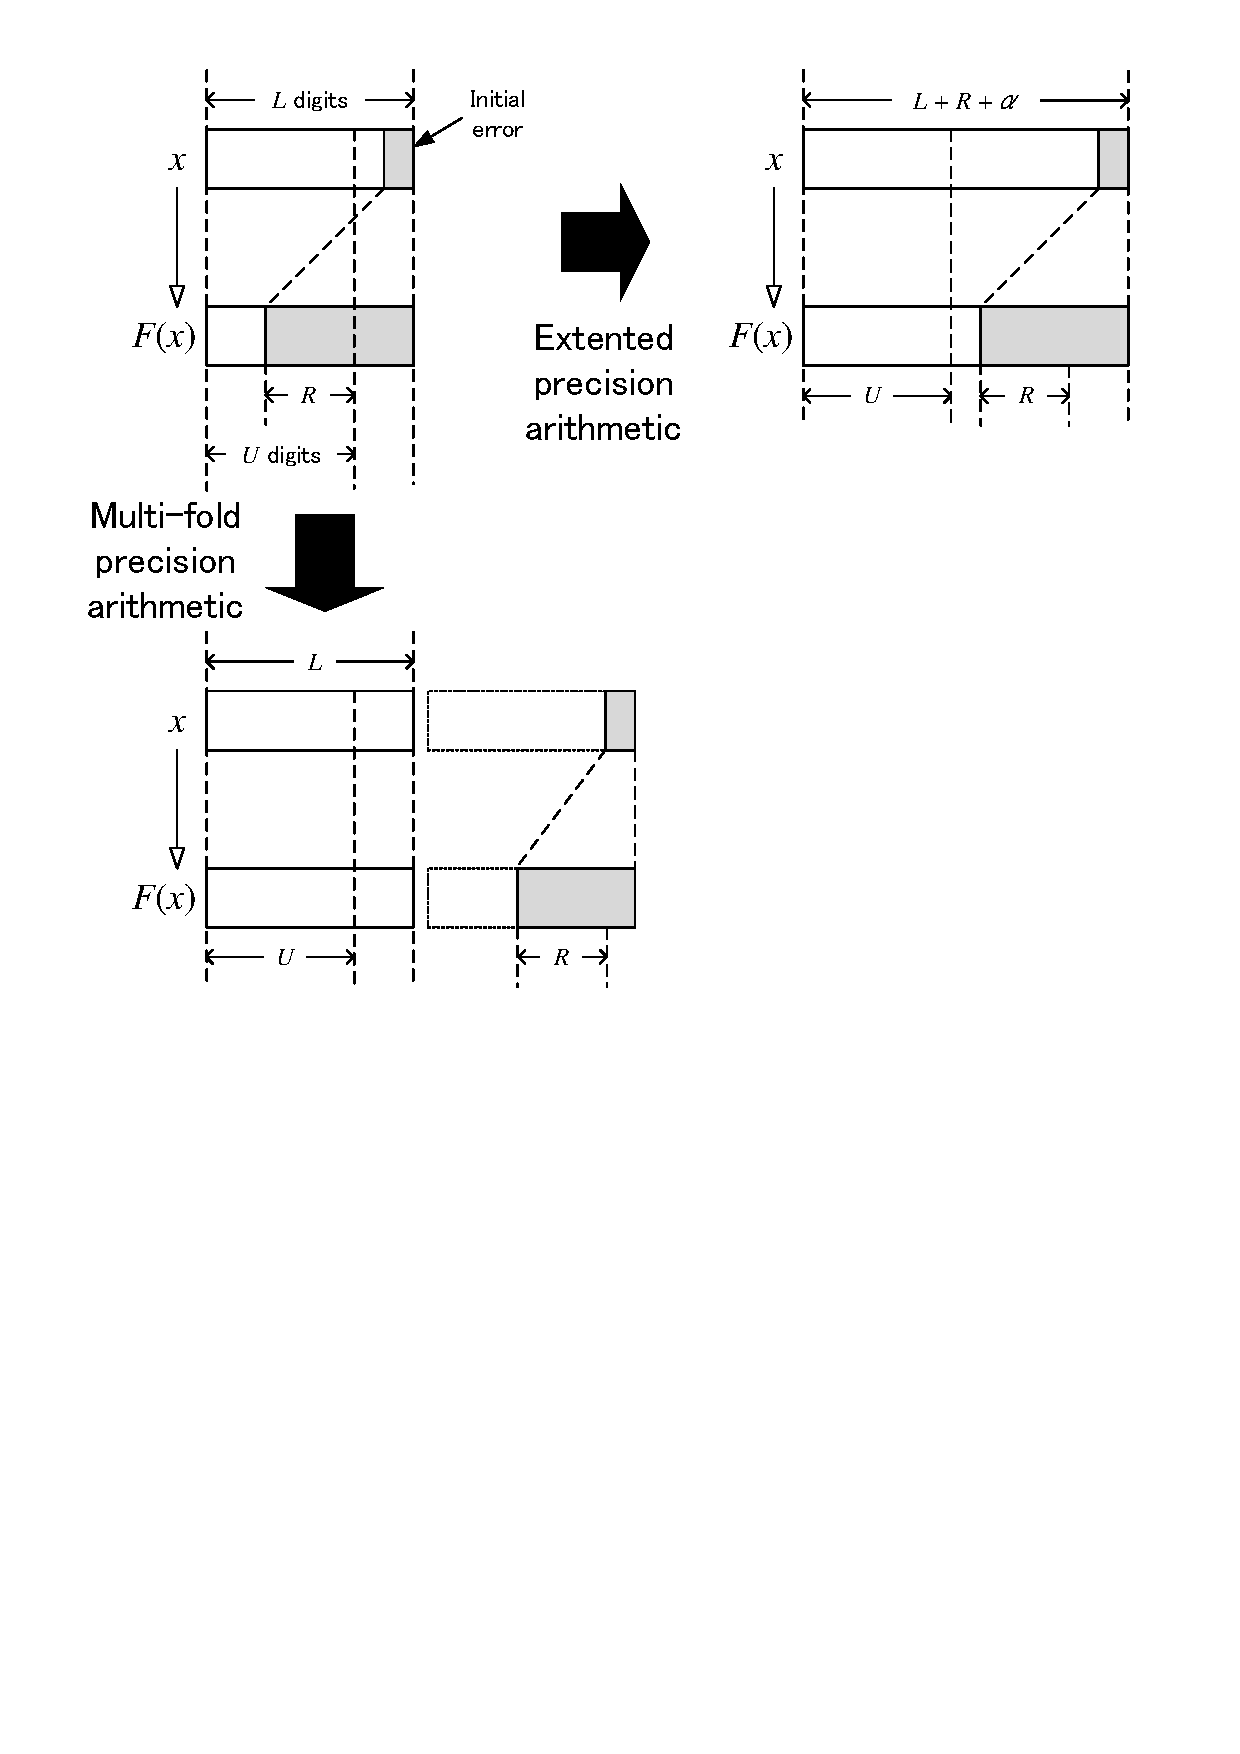
\includegraphics[width=.6\textwidth]{fig/multiprec_multifold.pdf}
        \caption{Extended precision and multi-fold precision arithmetics}
        \label{fig:multiprec_multifold}
    \end{center}
\end{figure}

\bi{Currently, not all algorithms used in numerical computation can be applied using multi-fold arithmetic, especially with nonlinear calculations. Therefore, it is necessary to employ a combination of multi-fold and multiple-precision calculations, where the basic linear calculation part, such as explicit extrapolation process solving initial value problems of ordinary differential equations, uses multi-fold calculations to reduce computational time.}{現在のところ、数値計算で用いられるすべてのアルゴリズム、特に非線形計算をmulti-fold演算で適用できるわけではありません。したがって、multi-foldと多倍長精度計算を組み合わせて用いる必要があり、常微分方程式の初期値問題を解く陽的補外法のような基本線形計算部分にmulti-fold計算を用いることで計算時間を削減します。}

\bi{The Ozaki scheme, a matrix multiplication algorithm that we incorporated into our library, is a technique based on the multi-fold calculation approach. By leveraging the speed of existing binary32 and binary64 xGEMM algorithms, it significantly optimizes multiple-precision matrix multiplication under certain conditions, as revealed in our benchmark and previous studies\cite{mukunoki_binary128}\cite{utsugiri_arxiv2023}. We are confident that the acceleration of multiple-precision linear computation libraries will remain an important theme in guaranteeing the accuracy of broader numerical computation algorithms, following the development trend of multiple-precision numerical algorithms.}{私たちがライブラリに組み込んだ行列乗算アルゴリズムであるOzaki schemeは、multi-fold計算アプローチに基づく技術です。既存のbinary32およびbinary64のxGEMMアルゴリズムの速度を活用することで、私たちのベンチマークおよび先行研究 \cite{mukunoki_binary128}\cite{utsugiri_arxiv2023} で明らかにされているように、特定の条件下で多倍長精度行列乗算を大幅に最適化します。私たちは、多倍長精度数値アルゴリズムの発展動向に従い、多倍長精度線形計算ライブラリの高速化が、より広範な数値計算アルゴリズムの精度保証において引き続き重要なテーマであり続けると確信しています。}

% ---------------------------------------
\section{\bi{Algorithms and performance of optimized matrix multiplication}{最適化された行列乗算のアルゴリズムと性能}}
% ---------------------------------------
\bi{We focused on the optimization of multiple-precision matrix multiplication, starting with MPI support for arbitrary-precision numerical calculations\cite{bnc}. Subsequently, owing to current popularity of multi-core CPUs, we accelerated multiple-precision matrix multiplication via parallelization support using OpenMP. As far as multiple-precision calculations are concerned, no other such results have been achieved by incorporating divide-and-conquer methods, such as the Strassen and Winograd algorithms. Although limited to multi-component methods, our proposed method is the only approach that supports AVX2 and has been converted to OpenMP for achieving higher speeds. However, the current code does not improve performance beyond eight threads for OpenMP acceleration, and a drastic reformulation is necessary to further improve parallelization performance. Algorithm\ \ref{algo:strassen} is the Strassen matrix multiplication.}{私たちは、任意精度数値計算のためのMPIサポート \cite{bnc} を皮切りに、多倍長精度行列乗算の最適化に注力してきました。その後、現在のマルチコアCPUの普及を背景に、OpenMPを用いた並列化サポートによって多倍長精度行列乗算を高速化しました。多倍長精度計算に関する限り、StrassenやWinogradアルゴリズムのような分割統治法を組み込んだ他の同様の成果は得られていません。multi-component方式に限られるものの、私たちの提案手法はAVX2をサポートし、高速化のためにOpenMP化された唯一のアプローチです。しかしながら、現在のコードはOpenMP高速化において8スレッドを超えると性能が向上せず、並列化性能をさらに改善するには抜本的な再構成が必要です。Algorithm\ \ref{algo:strassen} はStrassen行列乗算です。}

%\begin{figure}[htb]
\begin{algorithm}[htb]
    \algsetup{linenosize=\small}
    \small
    \caption{Strassen algorithm for matrix multiplication}\label{algo:strassen}
    \hspace*{\algorithmicindent} \textbf{Input:} $A = [A_{ij}]_{i,j=1,2}\in\mathbb{R}^{m\times l}$, $A_{ij}\in\mathbb{R}^{m/2\times l/2}$, $B = [A_{ij}]_{i,j=1,2}\in\mathbb{R}^{l\times n}$, $B_{ij}\in\mathbb{R}^{l/2\times n/2}$ \\
    \hspace*{\algorithmicindent} \textbf{Output:} $C := \mbox{Strassen}(A, B) = AB\in \mathbb{R}^{m\times n}$
    \begin{algorithmic}
        \IF{$m < m_0$ \&\& $n < n_0$}
            \STATE $C := AB$
        \ENDIF
        \STATE $P_1 := \mbox{Strassen}(A_{11} + A_{22}, B_{11} + B_{22})$
        \STATE $P_2 := \mbox{Strassen}(A_{21} + A_{22}, B_{11})$
        \STATE $P_3 := \mbox{Strassen}(A_{11}, B_{12} - B_{22})$
        \STATE $P_4 := \mbox{Strassen}(A_{22}, B_{21} - B_{11})$
        \STATE $P_5 := \mbox{Strassen}(A_{11} + A_{12}, B_{22})$
        \STATE $P_6 := \mbox{Strassen}(A_{21} - A_{11}, B_{11} + B_{12})$
        \STATE $P_7 := \mbox{Strassen}(A_{12} - A_{22}, B_{21} + B_{22})$
        \STATE $C_{11} := P_1 + P_4 - P_5 + P_7$; $C_{12} := P_3 + P_5$
        \STATE $C_{21} := P_2 + P_4$; $C_{22} := P_1 + P_3 - P_2 + P_6$
        \STATE $C := [C_{ij}]_{i,j=1,2}$
    \end{algorithmic}
\end{algorithm}
%\end{figure}

\bi{The usefulness of the Ozaki scheme is also clear at multiple-precision levels owing to the success of Mukunoki et al. in accelerating the float128 precision matrix multiplication\cite{mukunoki_binary128}.}{Ozaki schemeの有用性は、Mukunokiらによるfloat128精度行列乗算の高速化の成功 \cite{mukunoki_binary128} により、多倍長精度レベルにおいても明らかです。} %The float128 arithmetic, which is supported by GCC, exhibits TD to QD precision performance for addition and multiplication, and is expected to be appropriate for achieving precision levels within this range.
\bi{The float128 arithmetic supported by GCC features TD to QD precision performance for addition and multiplication and is likewise expected to be sufficient for this precision range.}{GCCがサポートするfloat128演算は、加算と乗算においてTDからQD精度の性能を備えており、同様にこの精度範囲に対して十分であると期待されます。}

\bi{The Ozaki scheme is an algorithm that aims to simultaneously accelerate performance and improve accuracy by dividing matrices into more matrices with elements represented by shorter digits. Similarly to the ``Split'' method used in the error-free transformation technique, this approach leverages on the speed of optimized short-precision matrix multiplication (xGEMM) functions. For a given matrix $A \in \mathbb{R}^{m\times l}$ and $B \in \mathbb{R}^{l\times n}$, to obtain a matrix product $C := AB \in \mathbb{R}^{m\times n}$ of long $L$-bit precision, $A$ and $B$ are divided using the Ozaki scheme, where $D \in \mathbb{N}$ is the maximum number of divisions of short $S$-bit precision matrices ($S << L$), as depicted in Algorithm\ \ref{algo:ozaki_scheme}. The $S$-bit arithmetic is used for calculations where no particular description is given, and the $L$-bit arithmetic is used only where high-precision operations are required.}{Ozaki schemeは、行列を、より短い桁で表現される要素を持つ多数の行列に分割することで、性能の高速化と精度の向上を同時に達成することを目指すアルゴリズムです。誤差なし変換技術で用いられる ``Split'' 法と同様に、このアプローチは最適化された短精度行列乗算 (xGEMM) 関数の速度を活用します。与えられた行列 $A \in \mathbb{R}^{m\times l}$ および $B \in \mathbb{R}^{l\times n}$ に対して、長い $L$ ビット精度の行列積 $C := AB \in \mathbb{R}^{m\times n}$ を得るために、Algorithm\ \ref{algo:ozaki_scheme} に示すように、$D \in \mathbb{N}$ を短い $S$ ビット精度行列 ($S << L$) の最大分割数として、$A$ と $B$ はOzaki schemeを用いて分割されます。特に記述のない計算には $S$ ビット演算が用いられ、$L$ ビット演算は高精度演算が必要な箇所でのみ用いられます。}

%\begin{figure}[htb]
\begin{algorithm}[htb]
    \algsetup{linenosize=\small}
    \small
    \caption{Ozaki scheme for multiple-precision matrix multiplication}\label{algo:ozaki_scheme}
	\hspace*{\algorithmicindent} \textbf{Input:} $A \in \mathbb{F}_{bL}^{m\times l}, B \in\mathbb{F}_{bL}^{l\times n}$ \\
	\hspace*{\algorithmicindent} \textbf{Output:} $C \in \mathbb{F}_{bL}^{m\times n}$
    \begin{algorithmic}
        \STATE $A^{(S)} := A$, $B^{(S)} := B$ : $A^{(S)} \in \mathbb{F}_{bS}^{m\times l}$, $B^{(S)} \in \mathbb{F}_{bS}^{l\times n}$
		% divide A and B
		\STATE $\mathbf{e} := [1\ 1\ ...\ 1]^T\in \mathbb{F}_{bS}^l$
		\STATE $\alpha := 1$
		\WHILE{$\alpha < D$}
			\STATE ${\boldsymbol\mu}_A := [\max_{1 \leq p \leq l} |(A^{(S)})_{ip}|]_{i=1, 2, ..., m} \in \mathbb{F}_{bS}^m$
			\STATE ${\boldsymbol\mu}_B := [\max_{1 \leq q \leq l} |(B^{(S)})_{qj}|]_{j=1, 2, ..., n} \in \mathbb{F}_{bS}^n$
			\STATE ${\boldsymbol\tau}_A := [2^{\lceil \log_2(({\boldsymbol\mu}_A)_i)\rceil + \lceil (S + \log_2(l)) / 2 \rceil} ]_{i = 1, 2, ..., m} \in \mathbb{F}_{bS}^m$
			\STATE ${\boldsymbol\tau}_B := [2^{\lceil \log_2(({\boldsymbol\mu}_B)_j)\rceil + \lceil (S + \log_2(l)) / 2 \rceil} ]_{j = 1, 2, ..., n} \in \mathbb{F}_{bS}^n$
			\STATE $S_A := \boldsymbol\tau_A \mathbf{e}^T$
			\STATE $S_B := \mathbf{e} \boldsymbol\tau_B^T$
			\STATE $A_\alpha := (A^{(S)} + S_A) - S_A$: $A_\alpha \in \mathbb{F}_{bS}^{m\times l}$
			\STATE $B_\alpha := (B^{(S)} + S_B) - S_B$: $B_\alpha \in \mathbb{F}_{bS}^{l\times n}$
			\STATE $A := A - A_\alpha$, $B := B - B_\alpha$ : $L$-bit FP arithmetic
			\STATE $A^{(S)} := A$, $B^{(S)} := B$
			\STATE $\alpha := \alpha + 1$  
		\ENDWHILE
		% multiplication
		\STATE $A_D := A^{(S)}$, $B_D := B^{(S)}$
		\STATE $C := O$
		\FOR{$\alpha = 1, 2, ..., D$}
			\FOR{$\beta = 1, 2, ..., D - \alpha + 1$}
				\STATE $C_{\alpha\beta} := A_\alpha B_\beta$
			\ENDFOR
			\STATE $C := C + \sum^{D - \alpha + 1}_{\beta = 1} C_{\alpha\beta}$ : $L$-bit FP arithmetic
		\ENDFOR
    \end{algorithmic}
\end{algorithm}
%\end{figure}

\bi{\figurename\ref{fig:ozaki_scheme3x3} illustrates an example of the Ozaki scheme when $A$ and $B\in\mathbb{R}^{3\times 3}$ are divided into three short-digit matrices.}{\figurename\ref{fig:ozaki_scheme3x3} は、$A$ と $B\in\mathbb{R}^{3\times 3}$ を3つの短桁行列に分割した場合のOzaki schemeの例を示しています。}
\begin{figure}[htb]
	\begin{center}
		%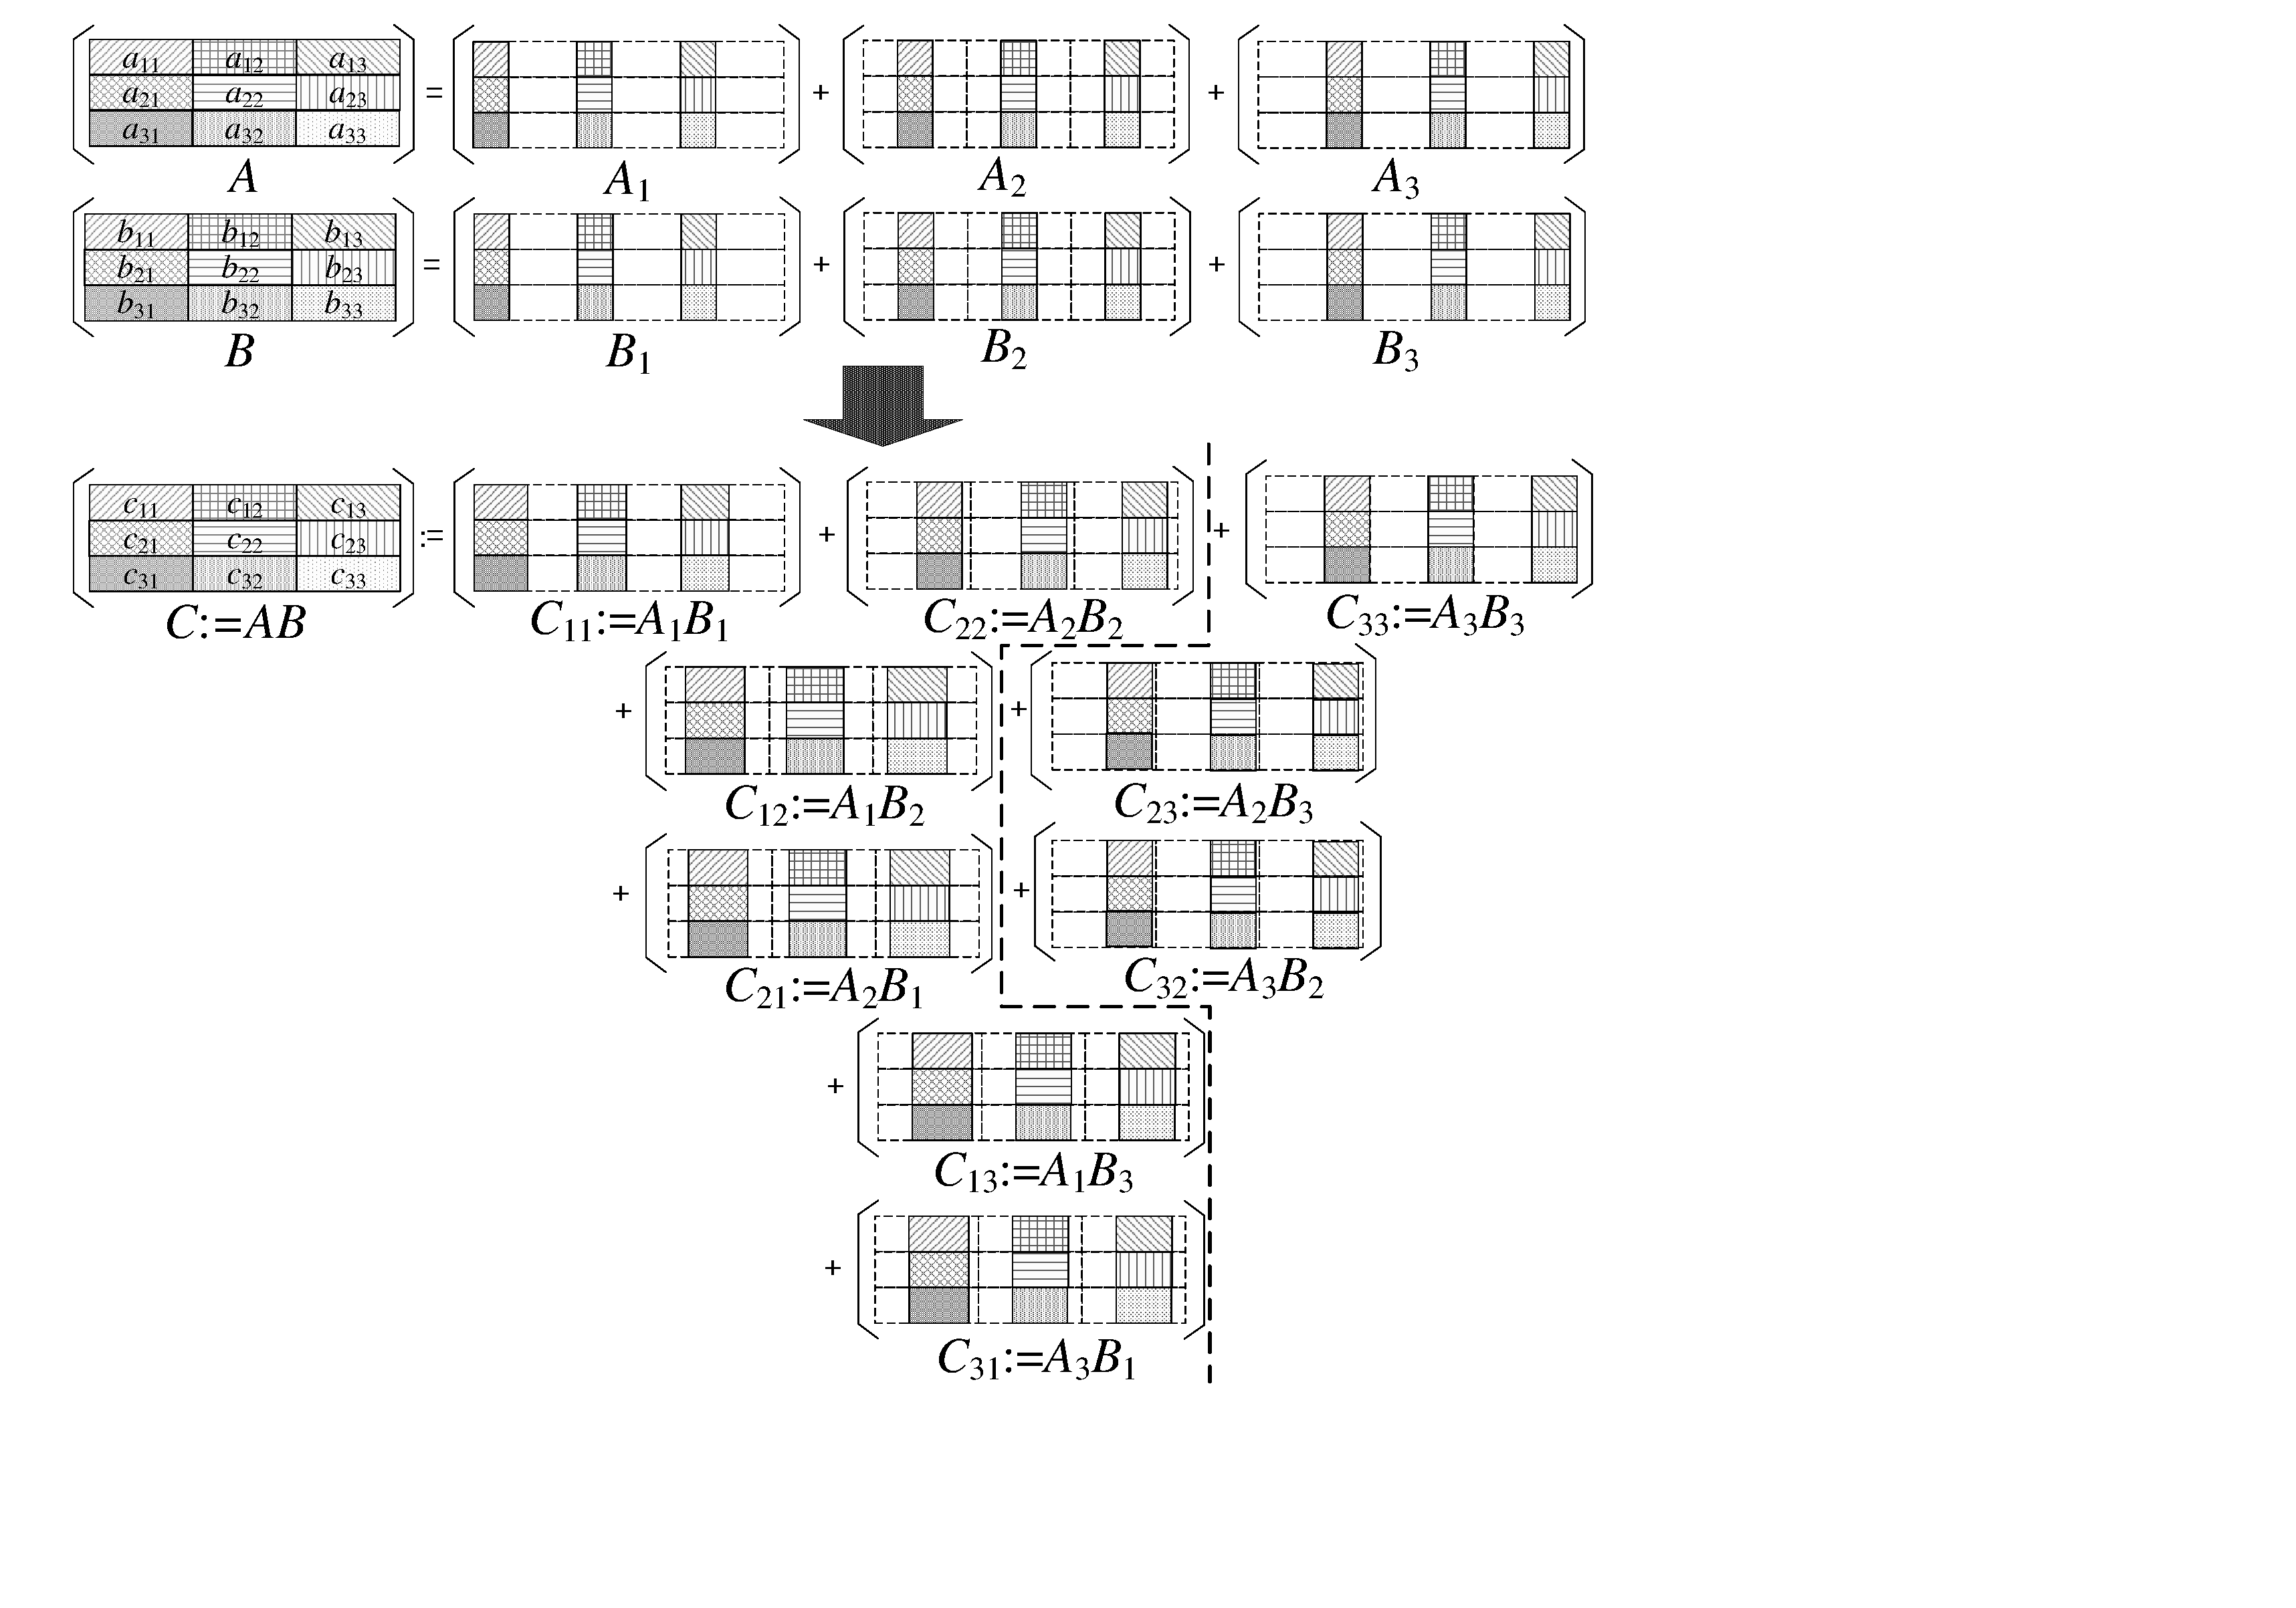
\includegraphics[width=.75\textwidth]{fig/ozaki_scheme_3x3.pdf}
		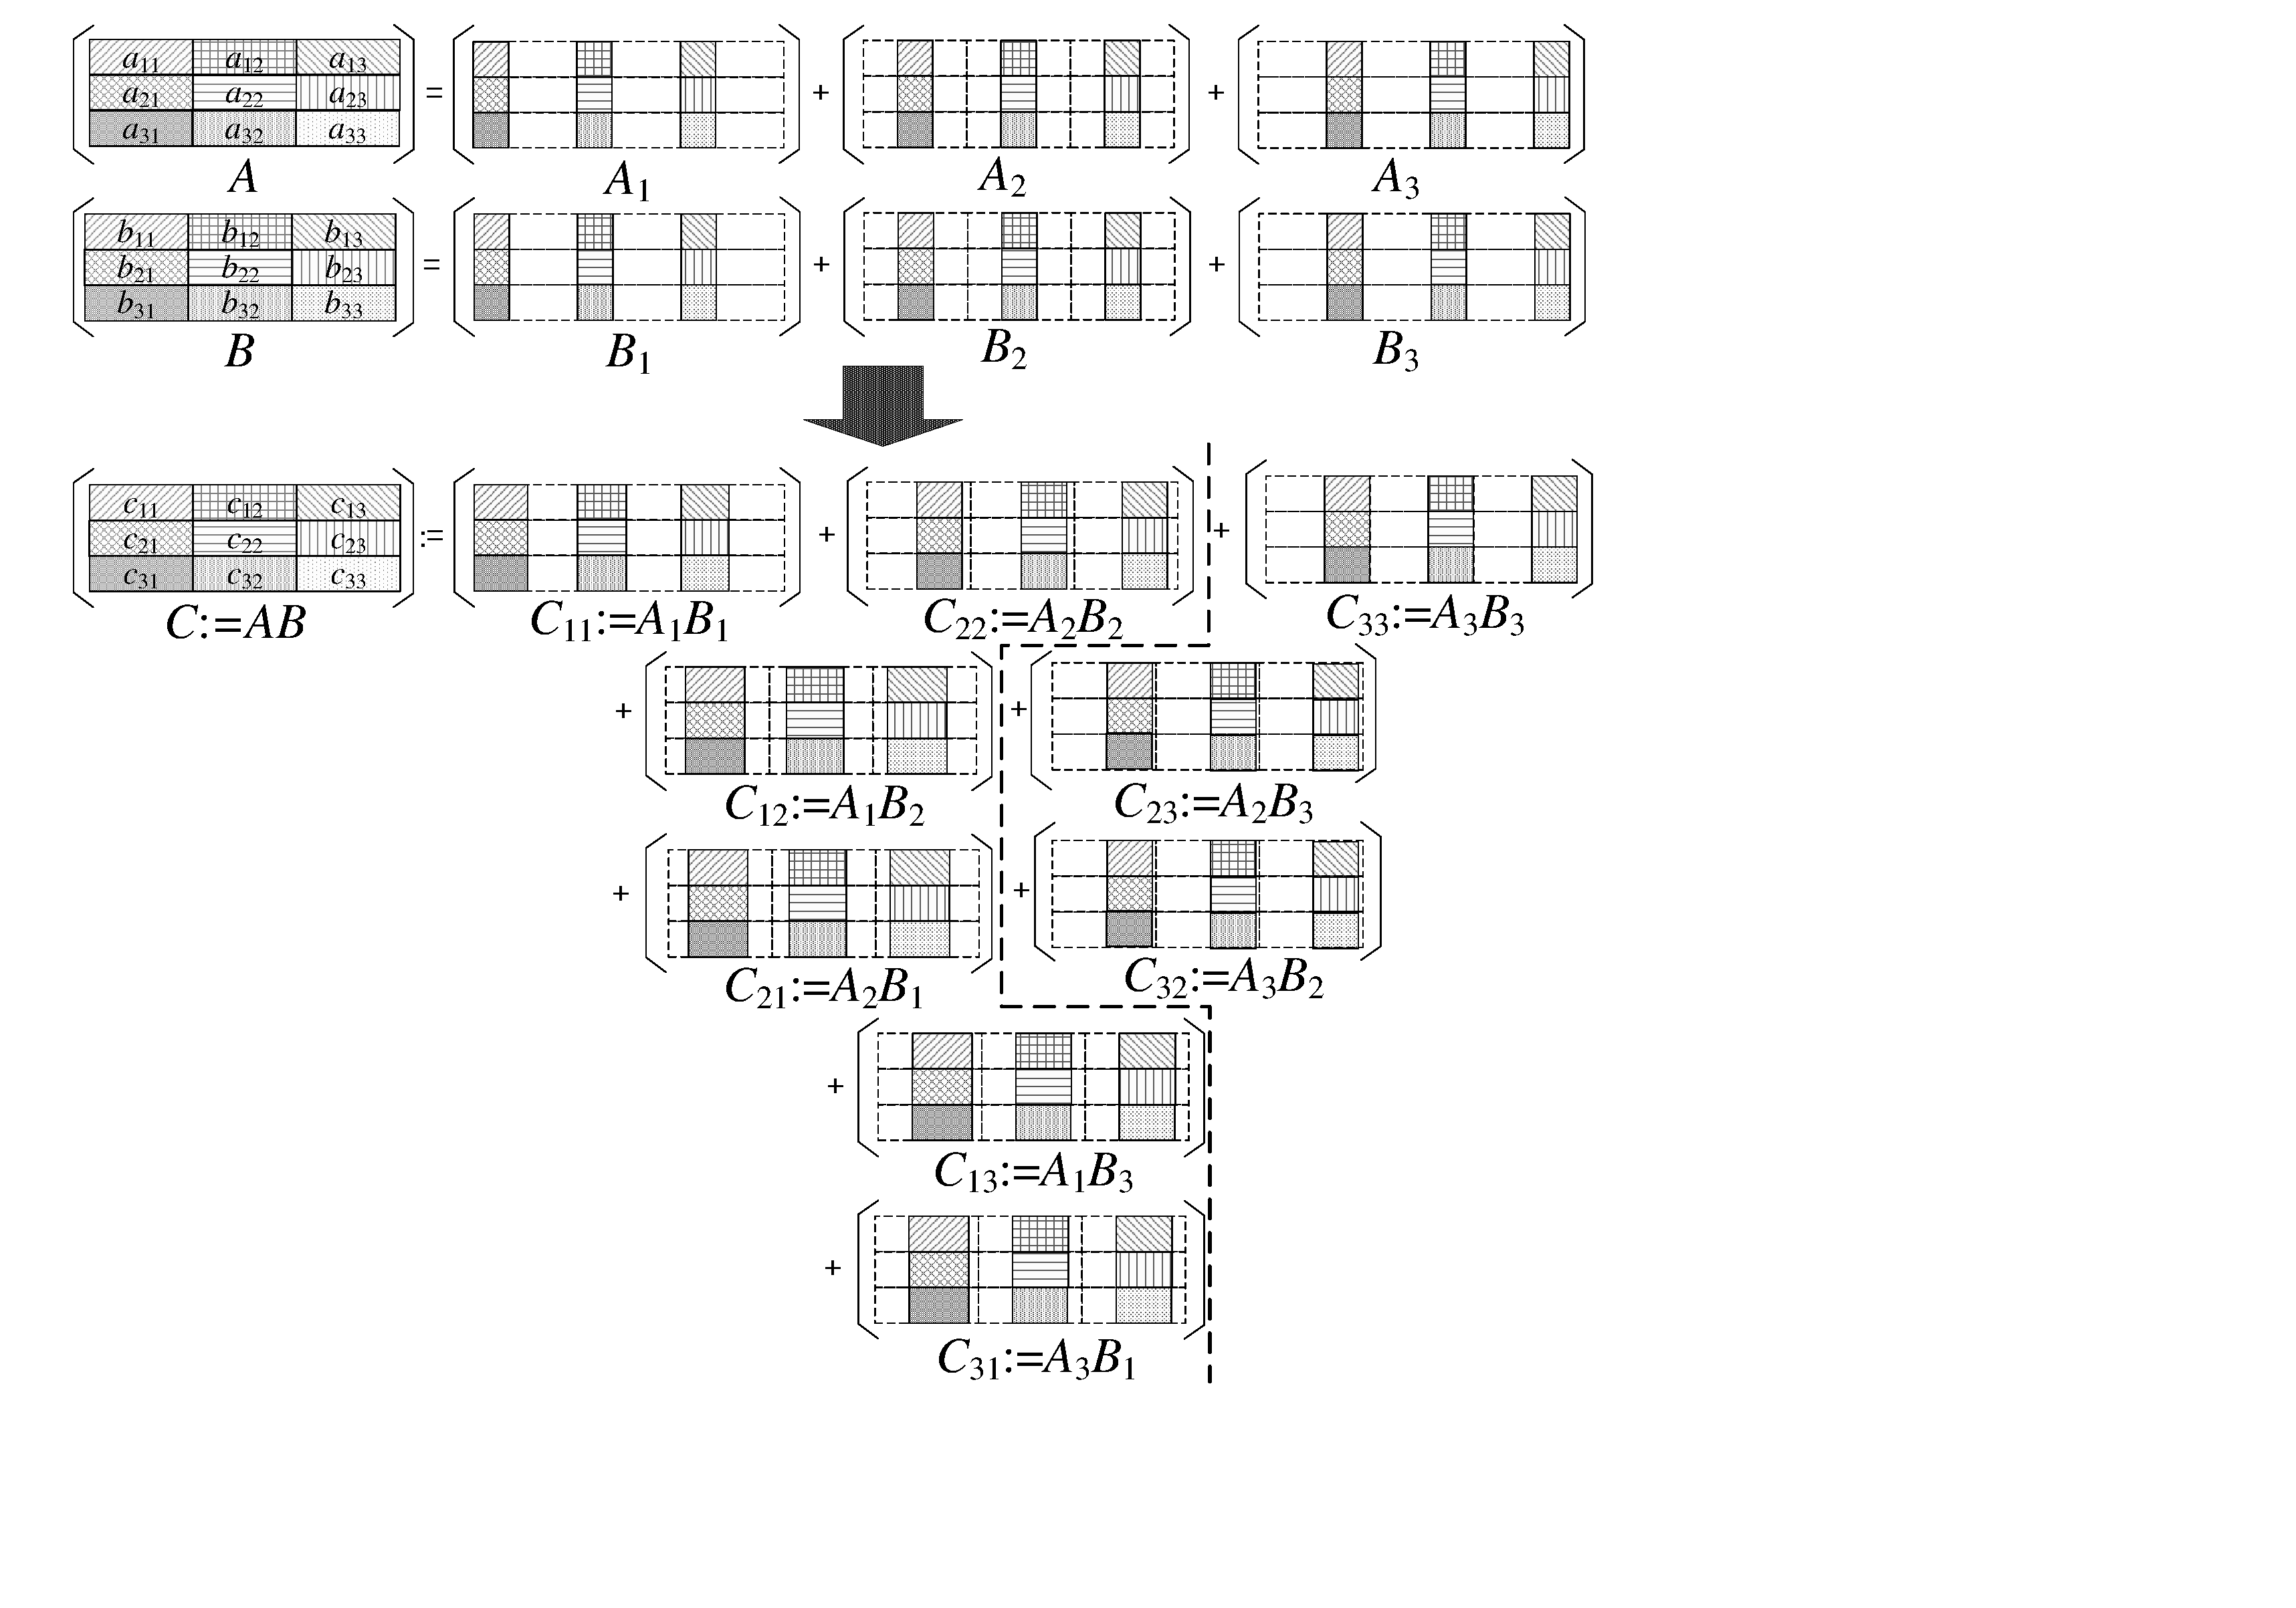
\includegraphics[width=.7\textwidth]{fig/ozaki_scheme_3x3.pdf}
        \caption{Matrix multiplication based on Ozaki scheme when the matrices are divided into three components}
		\label{fig:ozaki_scheme3x3}
	\end{center}
\end{figure}
\bi{The most important feature of the Ozaki scheme is that the matrices $A$ and $B$ are divided into $A_1$, $A_2$, $A_3$, $B_1$, $B_2$, and $B_3$ to fit within a short precision, thereby avoiding rounding errors in fast, low-precision matrix multiplication. An error-free matrix product $C_{ij} := A_i B_j$$(i,j=1, 2, 3)$ can be obtained as a result, and a highly accurate matrix product $C$ can be obtained using a multiple-precision matrix addition operation for $C := \sum_{i,j} C_{ij}$. Although the number of divisions of $A$ and $B$ is finite, it is difficult to determine the minimum number of divisions required to guarantee a certain accuracy threshold. As a result, benchmark tests must be performed to determine if the algorithm can be executed faster than other multiplication algorithms.}{Ozaki schemeの最も重要な特徴は、行列 $A$ と $B$ が短精度に収まるように $A_1$、$A_2$、$A_3$、$B_1$、$B_2$、$B_3$ に分割され、それによって高速な低精度行列乗算における丸め誤差を回避できる点です。その結果として誤差なし行列積 $C_{ij} := A_i B_j$$(i,j=1, 2, 3)$ を得ることができ、$C := \sum_{i,j} C_{ij}$ という多倍長精度行列加算演算を用いて高精度な行列積 $C$ を得ることができます。$A$ と $B$ の分割数は有限ですが、ある精度のしきい値を保証するために必要な最小分割数を決定することは困難です。その結果、このアルゴリズムが他の乗算アルゴリズムよりも高速に実行できるかどうかを判断するには、ベンチマークテストを行う必要があります。}

% ---------------------------------------
\section{\bi{Software layer of BNCmatmul}{BNCmatmulのソフトウェア層}}
% ---------------------------------------

\bi{We have already used QD\cite{qd} as multi-component-type fixed precision C++ class library, CAMPARY\cite{campary_paper2016} as multi-component-type arbitrary precision library, and MPFR\cite{mpfr} baased on GNU MP\cite{gmp}'s MPN kernel. MPLAPACK/MPBLAS\cite{mplapack} is greeding these all reliable MP libraries and providing the coresponding APIs of LAPACK/BLAS\cite{lapack}.}{私たちはこれまで、multi-component型固定精度C++クラスライブラリとしてQD \cite{qd}、multi-component型任意精度ライブラリとしてCAMPARY \cite{campary_paper2016}、そしてGNU MP \cite{gmp} のMPNカーネルに基づくMPFR \cite{mpfr} を用いてきました。MPLAPACK/MPBLAS \cite{mplapack} は、これらすべての信頼できる多倍長精度ライブラリを取り込み、LAPACK/BLAS \cite{lapack} に対応するAPIを提供しています。}
\bi{Our BNCmatmul developed aims to get better performance than MPBLAS as ATLAS, OpenBLAS and Intel Math Kernel, and it has the following features:}{私たちが開発したBNCmatmulは、ATLAS、OpenBLAS、Intel Math KernelのようにMPBLASよりも優れた性能を得ることを目指しており、以下の特徴を持ちます。}
\begin{itemize}
    \item \bi{Core functions and macros are wriiten in the traditional way of ANSI C, not C++.}{中核となる関数とマクロは、C++ではなく従来のANSI Cの流儀で書かれています。}
    \item \bi{Supporting native multi-component-type DD, TD, and QD precision arithmetic, and also accelelating vector and matrix computation like BLAS with AVX2 and AVX-512 on x86-64, and NEON and SVE2 on AArch64. As of 0.24 the AVX-512 backend covers every kernel the AVX2 backend does and is verified bit-identical to the scalar one (Sec.~\ref{sec:simdbackends}).}{ネイティブなmulti-component型のDD、TD、QD精度演算をサポートし、さらにx86-64ではAVX2とAVX-512、AArch64ではNEONとSVE2を用いてBLASのようにベクトルおよび行列計算を高速化します。0.24の時点でAVX-512バックエンドはAVX2バックエンドと同一のカーネルをすべて備え、スカラー版とのビット一致が検証されています（\ref{sec:simdbackends}節）。}
    \item \bi{Direct use of MPFR functions to avoid overhead due to mpreal class library.}{mprealクラスライブラリによるオーバーヘッドを回避するために、MPFR関数を直接利用します。}
    \item \bi{Supporting partly shared-memory-type parallelization based on OpenMP.}{OpenMPに基づく共有メモリ型並列化を部分的にサポートします。}
    \item \bi{Implementing three algorightms of matrix multiplication: simple triple-loop, blocking (tiling), and Strassen or Winograd algorithm. Ozaki scheme can be used as trial optimization.}{行列乗算の3つのアルゴリズム、すなわち単純な三重ループ、ブロック化 (タイリング)、およびStrassenまたはWinogradアルゴリズムを実装しています。Ozaki schemeは試験的な最適化として利用できます。}
\end{itemize}

\bi{The software layer of BNCmatmul except parallelization is shown as \figurename\ref{fig:lu_bench_layer}.}{並列化を除いたBNCmatmulのソフトウェア層を \figurename\ref{fig:lu_bench_layer} に示します。}

\begin{figure}[htb]
    \begin{center}
        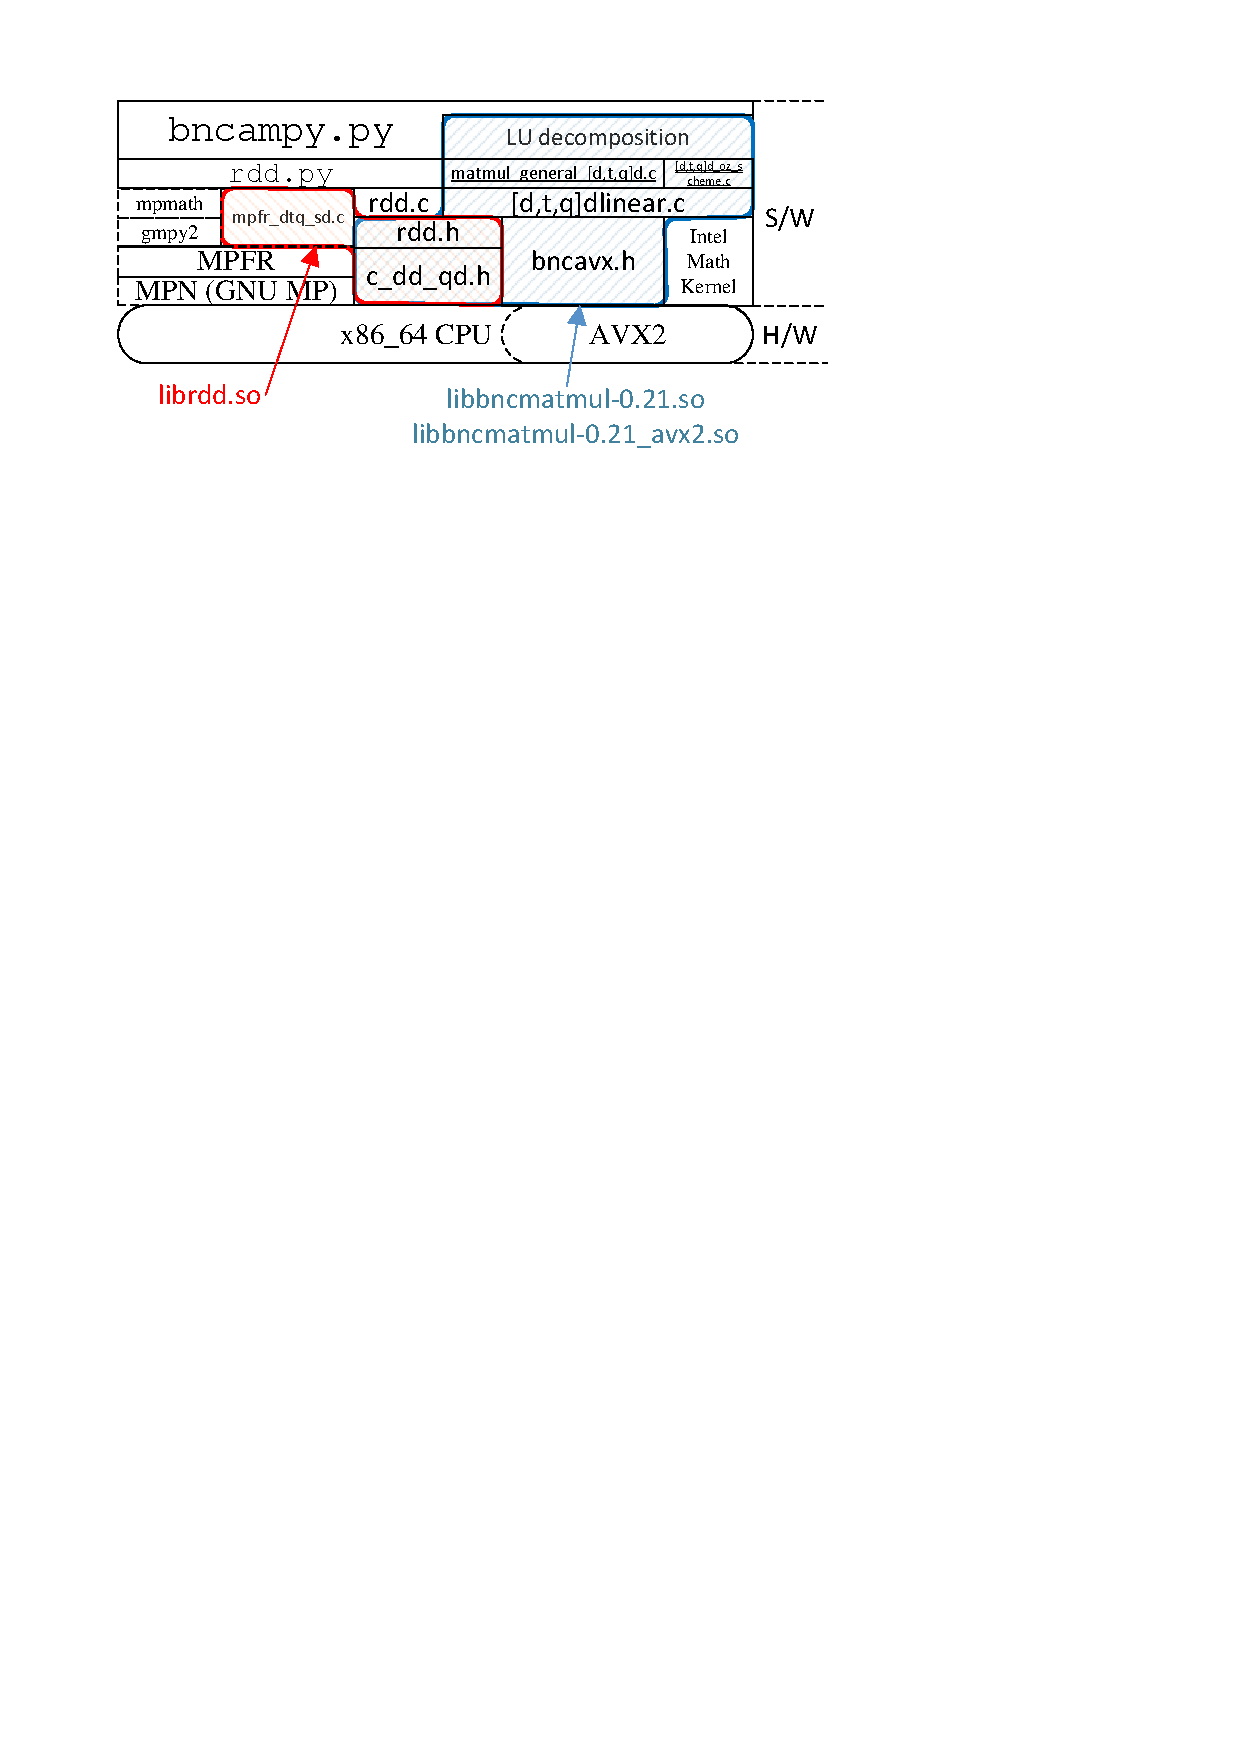
\includegraphics[width=.45\textwidth]{fig/pyrdd.pdf}
        \caption{Software layer of BNCmatmul library}
        \label{fig:lu_bench_layer}
    \end{center}
\end{figure}


\bi{Basic DD, TD, and QD precision arithmetic are defined as C inline functions in c\_dd\_qd.h and are defined as macros in rdd.h. To use the Python environment, rdd.c, which is based on rdd.h, is compiled as librdd.so. The DD, TD, and QD classes on Python use the functions defined in librdd.so.}{基本的なDD、TD、QD精度演算は、c\_dd\_qd.h内でCのinline関数として定義され、rdd.h内でマクロとして定義されています。Python環境を利用するために、rdd.hに基づくrdd.cがlibrdd.soとしてコンパイルされます。Python上のDD、TD、QDクラスは、librdd.so内で定義された関数を用います。}

\bi{BNCmatmul, which is also built on rdd.h and c\_dd\_qd.h, includes block and Strassen matrix multiplications that provide more efficient performance than simple triple-loop matrix multiplication. These have been accelerated using the SIMDized functions defined under include/avx2/ --- \texttt{\_bncavx\_*.h} for AVX2 (\texttt{\_\_m256d}/\texttt{\_\_m256}) and \texttt{\_bncavx\_*\_avx512.h} for AVX-512 (\texttt{\_\_m512d}/\texttt{\_\_m512}), both reached through the umbrella header avx2/bncavx.h --- and by their counterparts under include/neon/ and include/sve2/ on AArch64. The LU decomposition has also been accelerated in the same way.}{同じくrdd.hおよびc\_dd\_qd.h上に構築されたBNCmatmulには、単純な三重ループ行列乗算よりも効率的な性能を提供するブロック行列乗算およびStrassen行列乗算が含まれています。これらは、include/avx2/以下で定義されたSIMD化関数 --- AVX2用の \texttt{\_bncavx\_*.h}（\texttt{\_\_m256d}/\texttt{\_\_m256}）とAVX-512用の \texttt{\_bncavx\_*\_avx512.h}（\texttt{\_\_m512d}/\texttt{\_\_m512}）で、いずれもアンブレラヘッダ avx2/bncavx.h 経由で取り込まれます --- および、AArch64ではinclude/neon/・include/sve2/以下の対応する関数を用いて高速化されています。LU分解も同様に高速化されています。}

\bi{These functions that are defined in BNCmatmul (\figurename\ \ref{fig:lu_bench_layer}) can be used from libbncmatmul-0.xx.a/.so without any SIMDization techniques, and from libbncmatmul-0.xx\_avx2, \_avx512, \_neon, and \_sve2 with the SIMDization of AVX2, AVX-512, Arm NEON and Armv9-A SVE2, respectively. As these libraries have the same function names, so users do not need to modify their codes when selecting the BNCmatmul library --- the SIMD backend is chosen at link time only.}{BNCmatmul (\figurename\ \ref{fig:lu_bench_layer}) で定義されたこれらの関数は、SIMD化技術を用いないlibbncmatmul-0.xx.a/.so、およびAVX2・AVX-512・Arm NEON・Armv9-A SVE2によるSIMD化をそれぞれ用いたlibbncmatmul-0.xx\_avx2・\_avx512・\_neon・\_sve2から利用できます。これらのライブラリは同じ関数名を持つため、ユーザはBNCmatmulのライブラリを選択する際にコードを変更する必要はありません。SIMDバックエンドはリンク時にのみ選択されます。}


%------------------------------------------------%
% Todo list
%------------------------------------------------%
\section{\bi{History of Version and Todo list}{バージョン履歴とTodoリスト}}

\paragraph{\bi{History of Version}{バージョン履歴}}

\begin{description}
    \item[Version 0.24: 2026-08-15] \bi{Certified branch-free FMA and FMA-based elementary functions, ported from dtq-0.0.3 in plain ANSI C:}{dtq-0.0.3から純粋なANSI Cで移植した、証明付きbranch-free FMAとFMAベース初等関数:}
    \begin{enumerate}
        \item \bi{Branch-free fused multiply-add kernels \texttt{bnc\_\{dw,tw,qw\}fma[f]} with machine-proved error bounds (\texttt{bncfma.h}), including SIMD versions for NEON, SVE2, and --- newly --- AVX2/AVX-512 (\texttt{avx2/\_bncavx\_fma.h}); the NEON and AVX2 kernels are verified bit-identical to the scalar certified ones (Sec.~\ref{sec:bncfma})}{機械証明された誤差限界を持つbranch-free融合積和カーネル \texttt{bnc\_\{dw,tw,qw\}fma[f]}（\texttt{bncfma.h}）。NEON・SVE2に加え、新たにAVX2/AVX-512版（\texttt{avx2/\_bncavx\_fma.h}）を追加。NEON版・AVX2版はスカラー認証版とのビット一致を検証済み（\ref{sec:bncfma}節）}
        \item \bi{FMA-fused elementary functions $\exp$, $\mathrm{expm1}$, $\log$, $\log_{10}$, $\sin$, $\cos$, $\mathrm{sincos}$ for DD/TD/QD (DS/TS/QS by delegation), replacing the previous empty stubs and missing implementations of \texttt{c\_dd\_sin}, \texttt{c\_td\_*}, \texttt{c\_qd\_*}, etc.; accuracy validated against MPFR, average error below $1\,\varepsilon$ of each type (Sec.~\ref{sec:bncelem})}{DD/TD/QD向けFMA融合初等関数 $\exp$・$\mathrm{expm1}$・$\log$・$\log_{10}$・$\sin$・$\cos$・$\mathrm{sincos}$（DS/TS/QSは委譲）。従来の \texttt{c\_dd\_sin}・\texttt{c\_td\_*}・\texttt{c\_qd\_*} 等の空スタブ・未実装を置き換え。MPFR基準で精度検証済み、平均誤差は各型の$1\,\varepsilon$未満（\ref{sec:bncelem}節）}
        \item \bi{Elementwise array functions \texttt{bnc\_\{dd,td,qd\}\_\{exp,log,sin,cos\}\_array} over limb-planar arrays, blocked by the SIMD width of the build and bitwise identical to the scalar functions (Sec.~\ref{sec:bncelem})}{limb-planar配列に対する一括関数 \texttt{bnc\_\{dd,td,qd\}\_\{exp,log,sin,cos\}\_array}。ビルドのSIMD幅でブロック化され、スカラー関数とビット単位で一致（\ref{sec:bncelem}節）}
        \item \bi{Bug fixes: \texttt{const\_dd\_pi} held $\pi/16$, \texttt{const\_td\_pi}/\texttt{const\_qd\_pi} held $\pi/1024$, single-based $\pi$ constants were zero, and \texttt{c\_dd\_nint} was an empty stub}{バグ修正: \texttt{const\_dd\_pi} が$\pi/16$、\texttt{const\_td\_pi}/\texttt{const\_qd\_pi} が$\pi/1024$、float基の$\pi$定数がゼロ、\texttt{c\_dd\_nint} が空スタブだった問題}
        \item \bi{div/sqrt-safe FMA variants \texttt{bnc\_\{dw,tw,qw\}fma[f]\_safe} and the FMA-driven divisions \texttt{bnc\_\{dd,td,qd,ds,ts,qs\}\_div\_fma} (dtq \texttt{fma\_div} ports; opt-in default switch \texttt{BNC\_USE\_FMA\_DIV}); the double-based divisions run $1.2\times$/$2.8\times$/$2.2\times$ (DD/TD/QD) faster at the same accuracy (Sec.~\ref{sec:fmadiv})}{div/sqrt-safe版FMA \texttt{bnc\_\{dw,tw,qw\}fma[f]\_safe} とFMA駆動除算 \texttt{bnc\_\{dd,td,qd,ds,ts,qs\}\_div\_fma}（dtqの\texttt{fma\_div}移植。\texttt{BNC\_USE\_FMA\_DIV} で既定除算を切替可能）。double基の除算は同精度のまま$1.2$倍／$2.8$倍／$2.2$倍（DD/TD/QD）高速（\ref{sec:fmadiv}節）}
        \item \bi{AVX-512 backend brought to parity with AVX2: 411 of the 426 AVX2 constructs in the compiled sources now have a matching AVX-512 arm, the \texttt{avx512} build needs no ISA beyond AVX-512F + FMA, and the serial, AVX2 and AVX-512 builds are verified bit-identical on the element-wise and sparse kernels (Sec.~\ref{sec:simdbackends})}{AVX-512バックエンドをAVX2と同等に整備: ビルド対象ソース中426個のAVX2構文のうち411個が対応するAVX-512の腕を備え、\texttt{avx512} ビルドに必要なISAはAVX-512F + FMAのみ。serial・AVX2・AVX-512の各ビルドが要素毎カーネルおよび疎行列カーネルでビット一致することを検証済み（\ref{sec:simdbackends}節）}
        \item \bi{DLL-ready exported function API \texttt{rdd\_*}/\texttt{rtd\_*}/\texttt{rqd\_*}/\texttt{rds\_*}/\texttt{rts\_*}/\texttt{rqs\_*} (99 symbols, \texttt{src/rdtq\_func.c} + \texttt{include/rdtq\_func.h}) for Python/ctypes, with the \texttt{librdtq} build target and the \texttt{python/test\_rdtq.py} driver (Sec.~\ref{sec:rdtqfunc})}{Python/ctypes向けのDLL対応関数エクスポートAPI \texttt{rdd\_*}/\texttt{rtd\_*}/\texttt{rqd\_*}/\texttt{rds\_*}/\texttt{rts\_*}/\texttt{rqs\_*}（99シンボル、\texttt{src/rdtq\_func.c} + \texttt{include/rdtq\_func.h}）。\texttt{librdtq} ビルドターゲットと \texttt{python/test\_rdtq.py} ドライバ付き（\ref{sec:rdtqfunc}節）}
    \end{enumerate}
    \item[Version 0.23: 2026-03-16] \bi{BNCmatmul accelerated on Arm Neon CPUs has been released.}{Arm Neon CPU上で高速化されたBNCmatmulがリリースされました。}
    \item[Version 0.22: 2024-05-31] \bi{Some functions have been appended:}{いくつかの関数が追加されました。}
    \begin{enumerate}
        \item \bi{Complex arithmetic and linear computation}{複素数演算と線形計算}
        \item \bi{Miscellaneous functions (accessares, elementary and random functions) }{各種関数 (アクセサ、初等関数、乱数関数)}
        \item \bi{Sparse matrix and SpMV}{疎行列とSpMV}
    \end{enumerate}
    \item[Version 0.21: 2023-05-31] \bi{Secondly opening sources including DD, TD, QD and MPFR precision real BLAS functions at \url{https://github.com/tkouya/bncmatmul/blob/main/bncmatmul-0.21.tar.bz2}.}{DD、TD、QD、MPFR精度の実数BLAS関数を含むソースを \url{https://github.com/tkouya/bncmatmul/blob/main/bncmatmul-0.21.tar.bz2} で2回目に公開しました。}
    \item[Version 0.20: 2016-06-08] \bi{Firstly opening sources at \url{https://na-inet.jp/na/bnc/bncmatmul-0.2.tar.bz2}, which provides only artibrary matrix multiplication based on MPFR.}{MPFRに基づく任意精度行列乗算のみを提供するソースを \url{https://na-inet.jp/na/bnc/bncmatmul-0.2.tar.bz2} で初めて公開しました。}
\end{description}

\paragraph{\bi{Todo list}{Todoリスト}}

\begin{enumerate}
    %\item Appending complex BLAS functions with DD, TD, QD, and MPFR(MPC)
    %\item Appending complex LU decomposition and related functions
    %\item Appending sparse matrix-vector multiplication
    \item \bi{Showing more sample sources in this manual using BNCmatmul and MPLAPACK/BLAS}{本マニュアルにおいて、BNCmatmulとMPLAPACK/BLASを用いたサンプルソースをより多く示すこと}
    \item \bi{Completing descriptions of our library usage and how to apply various situations with it.}{本ライブラリの使用方法と、さまざまな状況への適用方法に関する説明を完成させること}
\end{enumerate}

%------------------------------------------------%
% End of Document
%------------------------------------------------%

%------------------------------------------------%
% Chap. 2 Basic Datatype and arithmetic
%------------------------------------------------%
%------------------------------------------------%
% Chap. 2
%------------------------------------------------%
\chapter{\bi{Basic datatypes and arithmetic}{基本データ型と算術演算}}\label{chap:basicarith}

\bi{In this chapter, we present and describe all basic data types and functions defined in BNCmatmul, and show how to use them in order to construct your programs including multiple-precsion computing.}{本章では、BNCmatmulで定義されているすべての基本データ型と関数を提示・説明し、多倍長精度計算を含むプログラムを構築するためのそれらの使い方を示します。}

\bi{As shown in Chapter 1, all basic datatype and functions are written in ANSI C, not C++ way.}{第1章で示したとおり、すべての基本データ型と関数はC++流ではなくANSI Cで記述されています。}

%------------------------------------------------%
% rdd.h -- the c_dd_* implementation layer (formerly c_dd_qd.h)
%------------------------------------------------%
\section{\bi{The \texttt{c\_dd\_*} arithmetic layer (\texttt{rdd.h})}{\texttt{c\_dd\_*}算術層（\texttt{rdd.h}）}}

\bi{Up to version 0.23 the macros and inline functions in this section were
provided by a separate header, \texttt{c\_dd\_qd.h} (and \texttt{c\_ds\_qs.h}
for the single-based family).  As of 0.24 both headers have been absorbed into
\texttt{rdd.h} and \texttt{rds.h} respectively, which are now the single
arithmetic headers of the multi-component families; including \texttt{rdd.h}
provides everything listed below.}{バージョン0.23まで、本節のマクロとinline関数は
独立したヘッダ\texttt{c\_dd\_qd.h}（単精度系は\texttt{c\_ds\_qs.h}）で提供されて
いました。0.24からは両ヘッダはそれぞれ\texttt{rdd.h}・\texttt{rds.h}に吸収され、
多倍長成分ファミリの算術ヘッダはこの2つに一本化されています。\texttt{rdd.h}を
includeすれば以下のすべてが利用できます。}

\begin{itemize} %  // return a * b + c
\macroitem{DFMA}{$a$, $b$, $c$} \bi{returns $a\times b + c$ in double precision}{倍精度で $a\times b + c$ を返します}
\macroitem{SFMA}{$a$, $b$, $c$} \bi{returns $a\times b + c$ in single precision}{単精度で $a\times b + c$ を返します}
\macroitem{QD\_FMA}{$a$, $b$, $c$} \bi{the same as}{次と同じです:} \macroname{DFMA}{$a$, $b$, $c$}
\macroitem{QD\_FMS}{$a$, $b$, $c$} \bi{returns $a \times b - c$ in double precision}{倍精度で $a \times b - c$ を返します}
\end{itemize}

\begin{itemize}
   \macroconstitem{DDSIZE} \bi{is 2, the number of binary64(double) variables in DD}{は2で、DD内のbinary64（double）変数の個数です}
   \macroconstitem{TDSIZE} \bi{is 3, the number of binary64 variables in TD}{は3で、TD内のbinary64変数の個数です}
   \macroconstitem{QDSIZE} \bi{is 4, the number of binary64 variables in QD}{は4で、QD内のbinary64変数の個数です}
\end{itemize}


\subsection{\bi{DD (double-double): 106-bit (53bits $\times$ 2) precision floating-point number}{DD（double-double）: 106ビット（53ビット $\times$ 2）精度浮動小数点数}}

\begin{itemize}
   \macroitem{DD\_HI}{a} is a[0]. 
   \macroitem{DD\_LOW}{a} is a[1].
   
   \macroconstitem{DD\_TRUE} is 1UL.
   \macroconstitem{TD\_TRUE}
   \macroconstitem{QD\_TRUE}
   \macroconstitem{DD\_FALSE} is 0UL.
   \macroconstitem{TD\_FALSE}
   \macroconstitem{QD\_FALSE}
   
   \macroitem{DD\_ISNAN}{a} \bi{checks if a includes NAN.}{a が NAN を含むかどうかを判定します。}
   \macroitem{TD\_ISNAN}{a}
   \macroitem{QD\_ISNAN}{a}
   \macroitem{DD\_ISINF}{a} \bi{checks if a includes INF.}{a が INF を含むかどうかを判定します。}
   \macroitem{TD\_ISINF}{a}
   \macroitem{QD\_ISINF}{a}
   \macroitem{DD\_ISZERO}{a} \bi{checks if a is zero.}{a がゼロかどうかを判定します。}
   \macroitem{TD\_ISZERO}{a}
   \macroitem{QD\_ISZERO}{a}
   \macroitem{DD\_ISONE}{a} \bi{checks if a is one.}{a が1かどうかを判定します。}
   \macroitem{TD\_ISONE}{a}
   \macroitem{QD\_ISONE}{a}
   \macroitem{DD\_ISNEGATIVE}{a} \bi{checks if a $< 0$.}{a $< 0$ かどうかを判定します。}
   \macroitem{TD\_ISNEGATIVE}{a}
   \macroitem{QD\_ISNEGATIVE}{a}
   \macroconstitem{DD\_NAN} is \verb|FP\_NAN|.
   \macroconstitem{TD\_NAN}
   \macroconstitem{QD\_NAN}

\end{itemize}

\section{\bi{Error-free transformation}{誤差なし変換（error-free transformation）}}

\begin{itemize}
   \funcitem{double}{quick\_two\_sum}{\varname{double}{$a$}, \varname{double}{$b$}, \varname{double *}{err}} $\cdots$ \bi{Computes fl($a+b$) and err($a+b$).  Assumes $|a| \geq |b|$.}{fl($a+b$) と err($a+b$) を計算します。$|a| \geq |b|$ を仮定します。}

   \funcitem{double}{quick\_two\_diff}{\varname{double}{a}, \varname{double}{b}, \varname{double *}{err}} $\cdots$  \bi{Computes fl($a-b$) and err($a-b$).  Assumes $|a| >= |b|$.}{fl($a-b$) と err($a-b$) を計算します。$|a| >= |b|$ を仮定します。}

   \funcitem{double}{two\_sum}{\varname{double}{a}, \varname{double}{b}, \varname{double *}{err}}$ \cdots$  \bi{Computes fl($a+b$) and err($a+b$).}{fl($a+b$) と err($a+b$) を計算します。}
   
   \funcitem{double}{two\_diff}{\varname{double}{a}, \varname{double}{b}, \varname{double *}{err}} $\cdots$  \bi{Computes fl($a-b$) and err($a-b$).}{fl($a-b$) と err($a-b$) を計算します。}

   \funcitem{void}{split}{\varname{double}{a}, double *hi, double *lo} $\cdots$ \bi{divide $a$ to hi and lo without error.}{$a$ を誤差なしで hi と lo に分割します。}

   \funcitem{double}{two\_prod}{\varname{double}{a}, \varname{double}{b}, \varname{double *}{err}} $\cdots$  \bi{Computes fl($ab$) and err($ab$).}{fl($ab$) と err($ab$) を計算します。}
   
   \funcitem{double}{two\_sqr}{\varname{double}{a}, \varname{double *}{err}} $\cdots$ \bi{Computes fl($a^2$) and err($a^2$). Faster than the above method.}{fl($a^2$) と err($a^2$) を計算します。上記の方法より高速です。}
   
\end{itemize}

\section{\bi{Double-double precision arithmetic}{double-double精度算術演算}}

\begin{itemize}
   \funcitem{dd\_bool}{dd\_is\_zero}{\varname{const double *}{x}} $\cdots$ \bi{Check if *x is zero.}{*x がゼロかどうかを判定します。}
   
   \funcitem{dd\_bool}{dd\_is\_one}{\varname{const double *}{x}}$\cdots$ \bi{Check if *x is one.}{*x が1かどうかを判定します。}
   
   \funcitem{void}{c\_dd\_set}{\varname{const double *}{x}, \varname{double}{*ret}}$\cdots$ $ret := x$
   
   \funcitem{void}{c\_dd\_set\_dd\_d}{\varname{const double}{x}, \varname{double *}{ret}} $\cdots$ $ret := (double)x$

   
   \funcitem{void}{c\_dd\_set0}{\varname{double *}{ret}} $\cdots$ $ret := 0$
   
   \funcitem{void}{c\_dd\_setnan}{\varname{double *}{ret}} $\cdots$ $ret := NaN$

   \funcitem{void}{c\_dd\_neg}{\varname{const double *}{a}, \varname{double *}{b}} $\cdots$ $b := -a$
   

   \funcitem{dd\_bool}{dd\_is\_positive}{\varname{const double *}{x}} $\cdots$ *x > 0 ?
   
   \funcitem{dd\_bool}{dd\_is\_negative}{\varname{const double *}{x}} $\cdots$ *x < 0 ?

   \funcitem{void}{c\_dd\_comp}{\varname{const double *}{a}, \varname{const double *}{b}, \varname{int *}{result}} $\cdots$ \bi{Compare with a and b, and store 0 if a == b, $+1$ else if a > b, $-1$ else if a < b.}{a と b を比較し、a == b なら 0、a > b なら $+1$、a < b なら $-1$ を格納します。}
   \funcitem{void}{c\_dd\_comp\_dd\_d}{\varname{const double *}{a}, \varname{double}{b}, \varname{int *}{result}}
   \funcitem{void}{c\_dd\_comp\_d\_dd}{\varname{double}{a}, \varname{const double *}{b}, \varname{int *}{result}}  
   \funcitem{void}{c\_dd\_pi}{\varname{double *}{a}}
   

   \funcitem{void}{c\_d\_add}{\varname{double}{a}, \varname{double}{b}, \varname{double *}{c}} $\cdots$ double-double := double + double

   \funcitem{void}{c\_dd\_add}{\varname{const double *}{a}, \varname{const double *}{b}, \varname{double *}{c}} $\cdots$ $ c:= a + b$
   \funcitem{void}{c\_dd\_add\_sloppy}{\varname{const double *}{a}, \varname{const double *}{b}, \varname{double *}{c}}  
   \funcitem{void}{c\_dd\_add\_dd\_d}{\varname{const double *}{a}, \varname{double}{b}, \varname{double *}{c}}
   \funcitem{void}{c\_dd\_add\_d\_dd}{\varname{double}{a}, \varname{const double *}{b}, \varname{double *}{c}}
   
   \funcitem{void}{c\_d\_sub}{\varname{double}{a}, \varname{double}{b}, \varname{double *}{c}} $\cdots$ double-double = double - double
   
   \funcitem{void}{c\_dd\_sub}{\varname{const double *}{a}, \varname{const double *}{b}, \varname{double *}{c}} $\cdots$ $c := a - b$
   \funcitem{void}{c\_dd\_sub\_sloppy}{\varname{const double *}{a}, \varname{const double *}{b}, \varname{double *}{c}}
   \funcitem{void}{c\_dd\_sub\_dd\_d}{\varname{const double *}{a}, \varname{double}{b}, \varname{double *}{c}}
   \funcitem{void}{c\_dd\_sub\_d\_dd}{\varname{double}{a}, \varname{const double *}{b}, \varname{double *}{c}}
  
   \funcitem{void}{c\_d\_mul}{\varname{double}{a}, \varname{double}{b}, \varname{double *}{c}} $\cdots$  double-double := double * double
   
   \funcitem{void}{c\_dd\_mul}{\varname{const double *}{a}, \varname{const double *}{b}, \varname{double *}{c}}
   \funcitem{void}{c\_dd\_mul\_dd\_d}{\varname{const double *}{a}, \varname{double}{b}, \varname{double *}{c}}
   \funcitem{void}{c\_dd\_mul\_d\_dd}{\varname{double}{a}, \varname{const double *}{b}, \varname{double *}{c}}

   \funcitem{void}{c\_d\_div}{\varname{double}{a}, \varname{double}{b}, \varname{double *}{c}} $\cdots $ $c := a / b$
  
   \funcitem{void}{c\_dd\_div}{\varname{const double *}{a}, \varname{const double *}{b}, \varname{double *}{c}} $\cdots $ $c := a / b$
   \funcitem{void}{c\_dd\_sloppy\_div}{\varname{double *}{a}, \varname{double *}{b}, \varname{double *}{c}}
   \funcitem{void}{c\_dd\_div\_dd\_d}{\varname{const double *}{a}, \varname{double}{b}, \varname{double *}{c}}
   \funcitem{void}{c\_dd\_div\_d\_dd}{\varname{double}{a}, \varname{const double *}{b}, \varname{double *}{c}}
   
   \funcitem{void}{c\_dd\_copy}{\varname{const double *}{a}, \varname{double *}{b}} $b := a$
   \funcitem{void}{c\_dd\_copy\_d}{\varname{double}{a}, \varname{double *}{b}}
   
   \funcitem{void}{c\_d\_sqr}{\varname{double}{a}, \varname{double *}{b}} $\cdots$  $b := a^2$
   \funcitem{void}{c\_dd\_sqr\_d}{\varname{double}{a}, \varname{double *}{ret}}
   \funcitem{void}{c\_dd\_sqr}{\varname{const double *}{a}, \varname{double *}{b}}

    \funcitem{void}{c\_dd\_sqrt}{\varname{const double *}{a}, \varname{double *}{b}} $\cdots $ $b := \sqrt(a)$
  
   \funcitem{void}{c\_dd\_abs}{\varname{const double *}{a}, \varname{double *}{b}} $\cdots $ $b := |a|$


   \funcitem{void}{c\_dd\_floor}{\varname{const double *}{a}, \varname{double *}{b}} $\cdots$ $b := \mbox{floor}(a)$

   \funcitem{void}{c\_dd\_ceil}{\varname{const double *}{a}, \varname{double *}{b}}$\cdots$ $b := \mbox{ceil}(a)$
 
\end{itemize}



\section{\bi{Quadruple-double precision arithmetic}{quadruple-double精度算術演算}}

\begin{itemize}

   \funcitem{void}{c\_qd\_copy}{\varname{const double *}{a}, \varname{double *}{b}} $\cdots$ $b := a$
   \funcitem{void}{c\_qd\_copy\_dd}{\varname{const double *}{a}, \varname{double *}{b}}
   \funcitem{void}{c\_qd\_copy\_d}{\varname{double}{a}, \varname{double *}{b}}
   
   \funcitem{void}{quick\_renorm}{\varname{double *}{c0}, \varname{double *}{c1}, \varname{double *}{c2}, \varname{double *}{c3}, \varname{double *}{c4}} $\cdots$ Renormalize c0 ... 
   \funcitem{void}{renorm}{\varname{double *}{c0}, \varname{double *}{c1}, \varname{double *}{c2}, \varname{double *}{c3}}
   \funcitem{void}{renorm4}{\varname{double *}{c0}, \varname{double *}{c1}, \varname{double *}{c2}, \varname{double *}{c3}, \varname{double *}{c4}}

   \funcitem{void}{three\_sum}{\varname{double *}{a}, \varname{double *}{b}, \varname{double *}{c}}
   
   \funcitem{void}{three\_sum2}{\varname{double *}{a}, \varname{double *}{b}, \varname{double *}{c}}
   
   \funcitem{void}{c\_qd\_add\_qd\_dd}{\varname{const double *}{a}, \varname{const double *}{b}, \varname{double *}{c}} $\cdots$ $ c := a + b$
   \funcitem{void}{c\_qd\_add}{\varname{const double *}{a}, \varname{const double *}{b}, \varname{double *}{c}}
   \funcitem{void}{c\_qd\_add\_sloppy}{\varname{const double *}{a}, \varname{const double *}{b}, \varname{double *}{c}} $\cdots$ \bi{not so accurate but fast addition}{精度はやや劣るものの高速な加算} $c := a + b$
   
   \funcitem{void}{c\_td\_addq}{\varname{const double *}{a}, \varname{const double *}{b}, \varname{double *}{c}} $\cdots$ \bi{triple double addition based on quad-double way}{quad-double方式に基づくtriple double加算}
   
   \funcitem{void}{c\_qd\_selfadd}{\varname{const double *}{a}, \varname{double *}{b}} $\cdots$ $ b := b + a$ 
   \funcitem{void}{c\_qd\_selfadd\_dd}{\varname{const double *}{a}, \varname{double *}{b}} 
   \funcitem{void}{c\_qd\_selfadd\_d}{\varname{double}{a}, \varname{double *}{b}}

    \funcitem{void}{c\_qd\_neg}{\varname{const double *}{a}, \varname{double *}{b}} $\cdots$ $b := -a$
   \funcitem{void}{c\_qd\_neg\_dd}{\varname{const double *}{a}, \varname{double *}{b}}
   \funcitem{void}{c\_qd\_neg\_d}{\varname{const double}{a}, \varname{double *}{b}}
   
   \funcitem{void}{c\_qd\_sub}{\varname{const double *}{a}, \varname{const double *}{b}, \varname{double *}{c}} $\cdots$ $c := a - b$
   \funcitem{void}{c\_qd\_sub\_qd\_dd}{\varname{const double *}{a}, \varname{const double *}{b}, \varname{double *}{c}}
   \funcitem{void}{c\_qd\_sub\_dd\_qd}{\varname{const double *}{a}, \varname{const double *}{b}, \varname{double *}{c}}
   \funcitem{void}{c\_qd\_sub\_qd\_d}{\varname{const double *}{a}, \varname{double}{b}, \varname{double *}{c}}
   \funcitem{void}{c\_qd\_sub\_d\_qd}{\varname{double}{a}, \varname{const double *}{b}, \varname{double *}{c}}
  
   \funcitem{void}{c\_qd\_selfsub}{\varname{const double *}{a}, \varname{double *}{b}} $\cdots$ $b := b + (-a) = b - a$
   \funcitem{void}{c\_qd\_selfsub\_dd}{\varname{const double *}{a}, \varname{double *}{b}}
   \funcitem{void}{c\_qd\_selfsub\_d}{\varname{double}{a}, \varname{double *}{b}}
   
   \funcitem{void}{c\_qd\_mul}{\varname{const double *}{a}, \varname{const double *}{b}, \varname{double *}{c}} $\cdots $ $c := a\times b$
   \funcitem{void}{c\_qd\_mul\_qd\_dd}{\varname{const double *}{a}, \varname{const double *}{b}, \varname{double *}{c}}
   \funcitem{void}{c\_qd\_mul\_dd\_qd}{\varname{const double *}{a}, \varname{const double *}{b}, \varname{double *}{c}}
   \funcitem{void}{c\_qd\_mul\_qd\_d}{\varname{const double *}{a}, \varname{double}{b}, \varname{double *}{c}}
   \funcitem{void}{c\_qd\_mul\_d\_qd}{\varname{double}{a}, \varname{const double *}{b}, \varname{double *}{c}}
   \funcitem{void}{c\_qd\_mul\_sloppy}{\varname{const double *}{a}, \varname{const double *}{b}, \varname{double *}{c}}

   \funcitem{void}{c\_qd\_sqr}{\varname{const double *}{a}, \varname{double *}{c}} $\cdots$ $c = a^2$

   \funcitem{void}{c\_qd\_selfmul}{\varname{const double *}{a}, \varname{double *}{b}} $\cdots$ $b := a * b$
   \funcitem{void}{c\_qd\_selfmul\_dd}{\varname{const double *}{a}, \varname{double *}{b}}
   \funcitem{void}{c\_qd\_selfmul\_d}{\varname{double}{a}, \varname{double *}{b}}

   \funcitem{void}{c\_qd\_div\_accurate}{\varname{const double *}{a}, \varname{const double *}{b}, \varname{double *}{c}} $\cdots$ $c:= a / b$
   \funcitem{void}{c\_qd\_div\_sloppy}{\varname{const double *}{a}, \varname{const double *}{b}, \varname{double *}{c}} $\cdots$ \bi{not so accurate but fast division (default)}{精度はやや劣るものの高速な除算（デフォルト）}

   \macroitem{USE\_QD\_DIV\_ACCURATE} $\cdots$ \bi{use accurate qd division if true}{真の場合、高精度なqd除算を使用します}
   
   \funcitem{void}{c\_qd\_div\_qd\_dd}{\varname{const double *}{a}, \varname{const double *}{b}, \varname{double *}{c}}
   \funcitem{void}{c\_qd\_div\_qd\_d}{\varname{const double *}{a}, \varname{double}{b}, \varname{double *}{c}}
   \funcitem{void}{c\_qd\_div\_d\_qd}{\varname{double}{a}, \varname{const double *}{b}, \varname{double *}{c}}

   
   \funcitem{void}{c\_qd\_selfdiv}{\varname{const double *}{a}, \varname{double *}{b}} $\cdots$ $ b := b / a$
   \funcitem{void}{c\_qd\_selfdiv\_dd}{\varname{const double *}{a}, \varname{double *}{b}}
   \funcitem{void}{c\_qd\_selfdiv\_d}{\varname{double}{a}, \varname{double *}{b}}
   
   \funcitem{void}{c\_qd\_mul\_pwr2}{\varname{const double *}{a}, \varname{double}{b}, \varname{double *}{c}} $\cdots$ $c := (a[0] * b, a[1] * b, a[2] * b, a[3] * b)$
 
   \funcitem{void}{c\_qd\_set}{\varname{const double *}{x}, \varname{double *}{qdval}} $\cdots$ 
    $qdval := c$

   
   \funcitem{void}{c\_qd\_set0{double *}{qdval}} $\cdots$ $qdval := 0$

   \funcitem{void}{c\_qd\_sqrt}{\varname{const double *}{a}, \varname{double *}{b}} $\cdots$ $b := \sqrt{a}$

   \funcitem{void}{c\_qd\_abs}{\varname{const double *}{a}, \varname{double *}{b}} $\cdots$ $b := |a|$
   
   \macroitem{nint}{a} $\cdots$ \bi{round($a$) as integer}{$a$ を整数に丸めます}
   \funcitem{void}{c\_qd\_nint}{\varname{const double *}{a}, \varname{double *}{b}}
   
   \funcitem{void}{c\_qd\_floor}{\varname{const double *}{a}, \varname{double *}{b}}$\cdots$ $b := \mbox{floor}(a)$
   \funcitem{void}{c\_qd\_ceil}{\varname{const double *}{a}, \varname{double *}{b}}$\cdots$ $b := \mbox{ceil}(a)$
   
  % \funcitem{void}{c\_qd\_aint}{\varname{const double *}{a}, \varname{double *}{b}}
    
   \funcitem{void}{c\_qd\_comp}{\varname{const double *}{a}, \varname{const double *}{b}, \varname{int *}{result}} $\cdots$ \bi{return -1 if $a < b$, 0 if $ a == b$, and +1 if $a > b$.}{$a < b$ なら -1、$ a == b$ なら 0、$a > b$ なら +1 を返します。}
   \funcitem{void}{c\_qd\_comp\_qd\_d}{\varname{const double *}{a}, \varname{double}{b}, \varname{int *}{result}}
   \funcitem{void}{c\_qd\_comp\_d\_qd}{\varname{double}{a}, \varname{const double *}{b}, \varname{int *}{result}}

\end{itemize}

\section{\bi{Triple-double precision arithmetic}{triple-double精度算術演算}}

\begin{itemize}

   \funcitem{void}{c\_td\_copy}{\varname{const double *}{a}, \varname{double *}{b}} $\cdots$ $b := a$
   \funcitem{void}{c\_qd\_copy\_td}{\varname{const double *}{a}, \varname{double *}{c}}
   \funcitem{void}{c\_td\_copy\_qd}{\varname{const double *}{a}, \varname{double *}{b}}
   \funcitem{void}{c\_td\_copy\_dd}{\varname{const double *}{a}, \varname{double *}{b}}
   \funcitem{void}{c\_td\_copy\_d}{\varname{double}{a}, \varname{double *}{b}}

   \funcitem{void}{vec\_sum}{double *e, \varname{const double *}{x}, \varname{int}{n}} $\cdots$ $ e[n] :={vec}\_sum(x[n])$

   \funcitem{void}{vseb}{\varname{double *}{y}, \varname{int}{ny}, \varname{const double *}{e}, \varname{int}{ne}} $\cdots$ $y[n] :={vec}\_sum\_err\_branch(vseb)(k)(e[n])$

   \funcitem{void}{c\_to\_td}{\varname{double *}{r}, \varname{double}{a}, \varname{double}{b}, \varname{double}{c}} $\cdots$  $r[3] := to\_td(a, b, c)$

   \funcitem{void}{merge}{\varname{double *}{c}, \varname{double *}{a}, int na, \varname{double *}{b}, \varname{int}{nb}} $\cdots$ \bi{Merge a[na] and b[nb] into c[na + nb]}{a[na] と b[nb] を c[na + nb] にマージします}

   
   \funcitem{void}{c\_td\_add}{\varname{double *}{a}, \varname{double *}{b}, \varname{double *}{c}} $\cdots$ $ c:= a + b$
   \funcitem{void}{c\_td\_add\_td\_d}{\varname{double *}{a}, \varname{double}{b}, \varname{double *}{c}}

   
   \funcitem{void}{c\_td\_neg}{\varname{const double *}{a}, \varname{double *}{c}} $\cdots$ $c := -a$

   //\funcitem{void}{c\_td\_sub}{\varname{double *}{c}, \varname{double *}{a}, \varname{double *}{b}} $\cdots$ $c := a - b$
   \funcitem{void}{c\_td\_sub}{\varname{double *}{a}, \varname{double *}{b}, \varname{double *}{c}}
   \funcitem{void}{c\_td\_subq}{\varname{const double *}{a}, \varname{const double *}{b}, \varname{double *}{c}}
   \funcitem{void}{c\_td\_sub\_d\_td}{\varname{double}{a}, \varname{double *}{b}, \varname{double *}{c}}
   //\funcitem{void}{c\_td\_sub\_td\_d}{\varname{double *}{c}, \varname{double *}{a}, \varname{double}{b}}
   \funcitem{void}{c\_td\_sub\_td\_d}{\varname{double *}{a}, \varname{double}{b}, \varname{double *}{c}}

   \funcitem{void}{c\_td\_mul\_accurate}{\varname{double *}{a}, \varname{double *}{b}, \varname{double *}{c}} $\cdots$ $c := a\times b$
   \funcitem{void}{c\_td\_mul\_sloppy}{\varname{double *}{a}, \varname{double *}{b}, \varname{double *}{c}} $\cdots$ \bi{not so accurate but fast}{精度はやや劣るものの高速} $c := a\times b$

   \macroitem{USE\_TD\_MUL\_ACCURATE} $\cdots$ \bi{Use accurate td multiplication if true}{真の場合、高精度なtd乗算を使用します}
   
   \funcitem{void}{c\_td\_mul\_dd\_td\_sloppy}{\varname{double *}{a}, \varname{double *}{b}, \varname{double *}{c}}
   \funcitem{void}{c\_td\_mul\_dd\_td\_accurate}{\varname{double *}{a}, \varname{double *}{b}, \varname{double *}{c}}

   
   \macroitem{USE\_TD\_MUL\_DD\_TD\_ACCURATE} $\cdots$ \bi{Use accurate td-dd multiplication if true}{真の場合、高精度なtd-dd乗算を使用します}
 
   
   \funcitem{void}{c\_td\_mul\_d\_td}{\varname{const double}{a}, \varname{const double *}{b}, \varname{double *}{c}}
  \funcitem{void}{c\_td\_mul\_td\_d}{\varname{const double *}{a}, const \varname{double}{b}, \varname{double *}{c}}

   
   \funcitem{void}{c\_td\_abs}{\varname{const double *}{a}, \varname{double *}{b}} $\cdots$ $b := |a|$

   \funcitem{void}{c\_td\_comp}{\varname{const double *}{a}, \varname{const double *}{b}, \varname{int *}{result}} $\cdots$ \bi{return -1 if $a < b$, 0 if $a == b$, and +1 if $a > b$.}{$a < b$ なら -1、$a == b$ なら 0、$a > b$ なら +1 を返します。}
   \funcitem{void}{c\_td\_comp\_td\_d}{\varname{const double *}{a}, \varname{double}{b}, \varname{int *}{result}}
   \funcitem{void}{c\_td\_comp\_d\_td}{\varname{double}{a}, \varname{const double *}{b}, \varname{int *}{result}}

   \funcitem{void}{c\_td\_2mtw\_dd\_td}{\varname{double}{a[DDSIZE]}, \varname{double}{b[TDSIZE]}, double c[TDSIZE]}
   
   \macroitem{ONE\_P\_2DBL\_EPS} $\cdots$ $1 + 2 \times$ DBL\_EPSILON $ = (1.00000000000000044e+00)$
   \macroitem{ONE\_M\_2DBL\_EPS} $\cdots$ $1 - 2 \times$ DBL\_EPSILON $ = (9.99999999999999556e-01)$
   
   \funcitem{void}{c\_td\_reci}{\varname{double *}{a}, \varname{double *}{c}}

   \funcitem{void}{c\_td\_divt}{\varname{double *}{a}, \varname{double *}{b}, \varname{double *}{c}}
  
   \macroitem{c\_td\_div} $\cdots$ \bi{the same as}{次と同じです:} \funcname{c\_td\_divtq}
   %\funcitem{void}{c\_td\_divtq}{\varname{double *}{a}, \varname{double *}{b}, \varname{double *}{c}}
   
   \funcitem{void}{c\_td\_divq}{\varname{const double *}{a}, \varname{const double *}{b}, \varname{double *}{c}} $\cdots$ \bi{td division based on quad-double division.}{quad-double除算に基づくtd除算です。}
   \funcitem{void}{c\_td\_div\_td\_d}{\varname{double *}{a}, \varname{double}{b}, \varname{double *}{c}}

   \funcitem{void}{c\_td\_sqrt}{\varname{double *}{a}, \varname{double *}{c}} $\cdots$ $c := \sqrt{a}$
   \funcitem{void}{c\_td\_sqrt\_d}{\varname{double}{a}, \varname{double *}{c}}   
   
   \funcitem{void}{c\_td\_sqr}{\varname{double *}{a}, \varname{double *}{c}} $\cdots$ $c := a^2$

\end{itemize}

%------------------------------------------------%
% bncfma.h : branch-free FMA (added in 0.24)
%------------------------------------------------%
\section{\bi{Branch-free fused multiply-add (\texttt{bncfma.h})}{Branch-free融合積和演算（\texttt{bncfma.h}）}}\label{sec:bncfma}

\bi{Version 0.24 provides certified branch-free fused multiply-add (FMA) kernels
$z := x \times y + c$ for DD/TD/QD (double-based) and DS/TS/QS (single-based)
arithmetic, ported operation-by-operation from the reference implementation of
T.~Kouya, ``Performance evaluation of branch-free fused multiply-add algorithms
for multi-component-type multiple-precision floating-point arithmetic''
(arXiv:2607.11391).  Each kernel matches an FPANVerifier-certified netlist and
carries a machine-proved error bound ($u = 2^{-p}$):}{バージョン0.24では、DD/TD/QD（double基）および
DS/TS/QS（float基）算術向けの、証明付き branch-free 融合積和演算（FMA）カーネル
$z := x \times y + c$ を提供します。T.~Kouya, ``Performance evaluation of
branch-free fused multiply-add algorithms for multi-component-type
multiple-precision floating-point arithmetic''（arXiv:2607.11391）の参照実装から
演算単位で忠実に移植したもので、各カーネルは FPANVerifier で認証されたネットリストに
一致し、機械証明された誤差限界（$u = 2^{-p}$）を持ちます。}

\begin{center}
\begin{tabular}{llll}
\hline
 & \bi{flops}{演算数} & \bi{certified error bound}{認証誤差限界} & \\
\hline
DW (DD/DS) & 17  & $|z - (xy+c)| \le 34 u^2 (|xy| + |c|)$ & \\
TW (TD/TS) & 66  & $|z - (xy+c)| \le 184 u^3 (|xy| + |c|)$ & \\
QW (QD/QS) & 146 & $|z - (xy+c)| \le 812 u^4 (|xy| + |c|)$ & \\
\hline
\end{tabular}
\end{center}

\begin{itemize}
   \funcitem{void}{bnc\_dwfma}{\varname{double}{z[2]}, \varname{const double}{x[2]}, \varname{const double}{y[2]}, \varname{const double}{c[2]}} $\cdots$ $z := x \times y + c$ (DD)
   \funcitem{void}{bnc\_twfma}{\varname{double}{z[3]}, \varname{const double}{x[3]}, \varname{const double}{y[3]}, \varname{const double}{c[3]}} $\cdots$ $z := x \times y + c$ (TD)
   \funcitem{void}{bnc\_qwfma}{\varname{double}{z[4]}, \varname{const double}{x[4]}, \varname{const double}{y[4]}, \varname{const double}{c[4]}} $\cdots$ $z := x \times y + c$ (QD)
   \funcitem{void}{bnc\_dwfmaf}{\varname{float}{z[2]}, \varname{const float}{x[2]}, \varname{const float}{y[2]}, \varname{const float}{c[2]}} $\cdots$ $z := x \times y + c$ (DS)
   \funcitem{void}{bnc\_twfmaf}{\varname{float}{z[3]}, \varname{const float}{x[3]}, \varname{const float}{y[3]}, \varname{const float}{c[3]}} $\cdots$ $z := x \times y + c$ (TS)
   \funcitem{void}{bnc\_qwfmaf}{\varname{float}{z[4]}, \varname{const float}{x[4]}, \varname{const float}{y[4]}, \varname{const float}{c[4]}} $\cdots$ $z := x \times y + c$ (QS)
\end{itemize}

\bi{The scalar kernels live in \texttt{bncfma\_d.h} / \texttt{bncfma\_f.h}
(umbrella header \texttt{bncfma.h}).  SIMD-vectorized versions with identical
semantics are provided for every backend: \texttt{neon/\_bncneon\_fma.h}
(\texttt{\_bncneon\_\{dw,tw,qw\}fma[f]}, \texttt{float64x2\_t}/\texttt{float32x4\_t}),
\texttt{sve2/\_bncsve2\_fma.h}, and --- new in 0.24 ---
\texttt{avx2/\_bncavx\_fma.h} with both AVX2
(\texttt{\_bncavx2\_\{dw,tw,qw\}fma[f]}, \texttt{\_\_m256d}/\texttt{\_\_m256}) and
AVX-512 (\texttt{\_bncavx512\_\{dw,tw,qw\}fma[f]}, \texttt{\_\_m512d}/\texttt{\_\_m512})
variants.  The NEON and AVX2 kernels have been verified bit-identical to the
scalar certified kernels over random operands; the AVX-512 build is covered
at the kernel level instead, by the whole-library bit-identity check of
Sec.~\ref{sec:simdbackends}.  All of them require
\texttt{-ffp-contract=off} (set by every BNCmatmul build): if the compiler
contracts $a \times b + c$ on its own, the error-free transformations inside
stop being error-free.}{スカラーカーネルは \texttt{bncfma\_d.h} / \texttt{bncfma\_f.h}
（アンブレラヘッダ \texttt{bncfma.h}）にあります。同一仕様のSIMD版を全バックエンドに
提供します: \texttt{neon/\_bncneon\_fma.h}
（\texttt{\_bncneon\_\{dw,tw,qw\}fma[f]}、\texttt{float64x2\_t}/\texttt{float32x4\_t}）、
\texttt{sve2/\_bncsve2\_fma.h}、および0.24で新規追加の \texttt{avx2/\_bncavx\_fma.h}
（AVX2版 \texttt{\_bncavx2\_\{dw,tw,qw\}fma[f]}（\texttt{\_\_m256d}/\texttt{\_\_m256}）と
AVX-512版 \texttt{\_bncavx512\_\{dw,tw,qw\}fma[f]}（\texttt{\_\_m512d}/\texttt{\_\_m512}））。
NEON版とAVX2版はランダムな被演算数に対してスカラー認証版と全limbビット一致することを
検証済みです。AVX-512ビルドについては、代わりに \ref{sec:simdbackends}節の
ライブラリ全体のビット一致検査でカーネルレベルの一致を確認しています。
いずれも \texttt{-ffp-contract=off} が必須です（BNCmatmulの全ビルドで
設定済み）。コンパイラが $a \times b + c$ を勝手に縮約すると、内部の誤差なし変換が
誤差なしでなくなるためです。}

\paragraph{\bi{div/sqrt-safe variants}{div/sqrt-safe変種}}

\bi{The certified bounds above are machine-proved for operands that are
normalized (non-overlapping) expansions.  The Newton iterations of division
and square root feed residuals that are \emph{not} non-overlapping, so no
FastTwoSum (\texttt{quick\_two\_sum}) precondition can be asserted for any
gate --- a FastTwoSum whose precondition fails does not even satisfy
$s + e = a + b$.  For such operands the \emph{safe} variants (ports of dtq's
\texttt{dw\_fma\_safe} / \texttt{tw\_fma\_safe} / \texttt{qw\_fma\_safe},
with a plain scalar multiplicand) demote every FastTwoSum to a full TwoSum
(DW: 20 flops); a safe variant is never cheaper, and never less accurate,
than the standard one.  They are consumed by the FMA-driven divisions
(Sec.~\ref{sec:bncelem}).}{上の認証誤差限界は、被演算数が正規化された
（non-overlappingな）多倍長展開であることを前提に機械証明されています。
除算・平方根のNewton反復に現れる残差はnon-overlappingとは限らないため、
どのゲートについてもFastTwoSum（\texttt{quick\_two\_sum}）の前提条件を
主張できません --- 前提条件が破れたFastTwoSumは $s + e = a + b$ すら
満たしません。このような被演算数向けに、\emph{safe}変種（dtqの
\texttt{dw\_fma\_safe} / \texttt{tw\_fma\_safe} / \texttt{qw\_fma\_safe} の
移植。第2被乗数はスカラー）はすべてのFastTwoSumを完全なTwoSumに置き換えます
（DW: 20 flops）。safe変種が標準版より速くなることはなく、また精度が落ちる
こともありません。FMA駆動除算（\ref{sec:bncelem}節）から使用されます。}

\begin{itemize}
   \funcitem{void}{bnc\_dwfma\_safe}{\varname{double}{z[2]}, \varname{const double}{x[2]}, \varname{double}{y}, \varname{const double}{c[2]}} $\cdots$ $z := x \times y + c$ \bi{(DD, scalar $y$)}{（DD、スカラー$y$）}
   \funcitem{void}{bnc\_twfma\_safe}{\varname{double}{z[3]}, \varname{const double}{x[3]}, \varname{double}{y}, \varname{const double}{c[3]}} $\cdots$ (TD)
   \funcitem{void}{bnc\_qwfma\_safe}{\varname{double}{z[4]}, \varname{const double}{x[4]}, \varname{double}{y}, \varname{const double}{c[4]}} $\cdots$ (QD)
   \funcitem{void}{bnc\_dwfmaf\_safe}{\varname{float}{z[2]}, \varname{const float}{x[2]}, \varname{float}{y}, \varname{const float}{c[2]}} $\cdots$ (DS)
   \funcitem{void}{bnc\_twfmaf\_safe}{\varname{float}{z[3]}, \varname{const float}{x[3]}, \varname{float}{y}, \varname{const float}{c[3]}} $\cdots$ (TS)
   \funcitem{void}{bnc\_qwfmaf\_safe}{\varname{float}{z[4]}, \varname{const float}{x[4]}, \varname{float}{y}, \varname{const float}{c[4]}} $\cdots$ (QS)
\end{itemize}

\bi{Defining \texttt{BNC\_USE\_NEW\_FMA} at library build time switches
\texttt{rdd\_fma}/\texttt{rtd\_fma}/\texttt{rqd\_fma} (and the \texttt{rds}/%
\texttt{rts}/\texttt{rqs} counterparts) plus the AXPY / dot product / GEMV /
GEMM / polynomial-evaluation call sites in the serial, NEON and SVE2 paths to
these kernels; without the macro the library is bit-for-bit unchanged.}{ライブラリの
ビルド時に \texttt{BNC\_USE\_NEW\_FMA} を定義すると、
\texttt{rdd\_fma}/\texttt{rtd\_fma}/\texttt{rqd\_fma}（および \texttt{rds}/%
\texttt{rts}/\texttt{rqs} 系）と、serial・NEON・SVE2パスの AXPY・内積・GEMV・GEMM・
多項式評価の呼び出し箇所がこれらのカーネルに切り替わります。マクロ未定義の場合、
ライブラリはビット単位で従来と同一です。}

%------------------------------------------------%
% bncelem.h : FMA-based elementary functions (added in 0.24)
%------------------------------------------------%
\section{\bi{FMA-based elementary functions (\texttt{bncelem.h})}{FMAベース初等関数（\texttt{bncelem.h}）}}\label{sec:bncelem}

\bi{Version 0.24 ports the FMA-fused elementary functions of dtq-0.0.3 to plain
ANSI C: proper argument reduction ($\ln 2$ reduction with repeated squaring or
two-level $\exp$ tables; $2\pi \to \pi/2 \to \pi/16$ or $\pi/1024$ reduction
with 256-entry tables for trigonometric functions) followed by Taylor kernels
whose terms are each accumulated with one certified branch-free FMA
(Sec.~\ref{sec:bncfma}) instead of a separate multiply and add.  The coefficient
tables (\texttt{bncelem\_tables.h}) are extracted mechanically from the
dtq-0.0.3 sources; the TD tables reproduce dtq's \texttt{to\_td\_real()}
folding of the QD tables exactly.  Accuracy has been validated against MPFR
(512-bit) references: the average relative error is below $1\,\varepsilon$ of
each type ($\varepsilon_{\rm DD} = 2^{-104}$, $\varepsilon_{\rm TD} = 2^{-157}$,
$\varepsilon_{\rm QD} = 2^{-209}$), equivalent to dtq itself.}{バージョン0.24では、
dtq-0.0.3のFMA融合初等関数を純粋なANSI Cに移植しました。適切な引数簡約
（$\ln 2$簡約＋反復自乗、または2段の$\exp$表；三角関数は
$2\pi \to \pi/2 \to \pi/16$ または $\pi/1024$ 簡約＋256エントリ表）の後、
Taylor級数の各項を乗算・加算の分離実行ではなく、証明付き branch-free FMA
（\ref{sec:bncfma}節）1回で積算します。係数表（\texttt{bncelem\_tables.h}）は
dtq-0.0.3のソースから機械的に抽出したもので、TD用の表はQD表に対するdtqの
\texttt{to\_td\_real()} 折り畳みを厳密に再現しています。精度はMPFR（512ビット）を
基準に検証済みで、平均相対誤差は各型の $1\,\varepsilon$ 未満
（$\varepsilon_{\rm DD} = 2^{-104}$、$\varepsilon_{\rm TD} = 2^{-157}$、
$\varepsilon_{\rm QD} = 2^{-209}$）であり、dtq本体と同等です。}

\subsection{\bi{Scalar functions}{スカラー関数}}

\bi{For each double-based type the following functions are provided
(\texttt{include/bncelem\_dd.h} / \texttt{\_td.h} / \texttt{\_qd.h}; umbrella
header \texttt{bncelem.h}).  The prefix is \texttt{bnc\_dd\_}, \texttt{bnc\_td\_}
or \texttt{bnc\_qd\_} and the limb count $K$ is 2, 3 or 4:}{各double基型に対して
以下の関数を提供します（\texttt{include/bncelem\_dd.h} / \texttt{\_td.h} /
\texttt{\_qd.h}、アンブレラヘッダは \texttt{bncelem.h}）。接頭辞は
\texttt{bnc\_dd\_}、\texttt{bnc\_td\_}、\texttt{bnc\_qd\_}、limb数$K$はそれぞれ
2、3、4です:}

\begin{itemize}
   \funcitem{void}{bnc\_dd\_exp}{\varname{const double *}{x}, \varname{double *}{ret}} $\cdots$ $ret := \exp(x)$
   \funcitem{void}{bnc\_dd\_expm1}{\varname{const double *}{x}, \varname{double *}{ret}} $\cdots$ $ret := \exp(x) - 1$ \bi{(accurate for small $|x|$)}{（小さい$|x|$で高精度）}
   \funcitem{void}{bnc\_dd\_log}{\varname{const double *}{x}, \varname{double *}{ret}} $\cdots$ $ret := \log_e(x)$ \bi{(one Newton step on $\exp$)}{（$\exp$に対するNewton法1回）}
   \funcitem{void}{bnc\_dd\_log10}{\varname{const double *}{x}, \varname{double *}{ret}} $\cdots$ $ret := \log_{10}(x)$
   \funcitem{void}{bnc\_dd\_sin}{\varname{const double *}{x}, \varname{double *}{ret}} $\cdots$ $ret := \sin(x)$
   \funcitem{void}{bnc\_dd\_cos}{\varname{const double *}{x}, \varname{double *}{ret}} $\cdots$ $ret := \cos(x)$
   \funcitem{void}{bnc\_dd\_sincos}{\varname{const double *}{x}, \varname{double *}{sin\_x}, \varname{double *}{cos\_x}} $\cdots$ \bi{computes $\sin(x)$ and $\cos(x)$ simultaneously}{$\sin(x)$と$\cos(x)$を同時に計算します}
   \funcitem{void}{bnc\_dd\_nint}{\varname{const double *}{x}, \varname{double *}{ret}} $\cdots$ \bi{nearest integer}{最近接整数}
\end{itemize}

\bi{The same set exists as \texttt{bnc\_td\_*} and \texttt{bnc\_qd\_*} with
3- and 4-limb arrays.  The single-based types delegate to the double-based
implementations exactly as in dtq (\texttt{bncelem\_f.h}):
\texttt{bnc\_ds\_*} $\to$ DD, \texttt{bnc\_ts\_*} $\to$ TD,
\texttt{bnc\_qs\_*} $\to$ QD, with exact limb conversions in both
directions.}{同じ関数群が3-limb/4-limb配列版の \texttt{bnc\_td\_*}・\texttt{bnc\_qd\_*}
として存在します。float基型はdtqと同様にdouble基実装へ委譲します
（\texttt{bncelem\_f.h}）: \texttt{bnc\_ds\_*} $\to$ DD、\texttt{bnc\_ts\_*} $\to$ TD、
\texttt{bnc\_qs\_*} $\to$ QD。limb変換は双方向とも厳密です。}

\subsection{\bi{Wiring into the \texttt{c\_dd\_*} / \texttt{c\_td\_*} / \texttt{c\_qd\_*} interfaces}{\texttt{c\_dd\_*}／\texttt{c\_td\_*}／\texttt{c\_qd\_*}インタフェースへの接続}}

\bi{Up to version 0.23 most of the elementary functions declared in
\texttt{c\_dd\_qd.h} and \texttt{c\_ds\_qs.h} were \emph{empty stubs} whose
bodies were disabled by \texttt{\#if 0} (\texttt{c\_dd\_sin}, \texttt{c\_dd\_cos},
\texttt{c\_dd\_tan}, \texttt{c\_dd\_sincos}, \texttt{c\_dd\_nint}, all
\texttt{c\_qd\_*} and \texttt{c\_qs\_*}/\texttt{c\_ds\_*} elementary functions),
and the \texttt{c\_td\_*}/\texttt{c\_ts\_*} elementary functions referenced from
\texttt{rdd.h}/\texttt{rds.h} did not exist at all.  As of 0.24 every one of
them delegates to the corresponding \texttt{bnc\_*} implementation.
The previous working implementations are kept for comparison purposes under the
names \texttt{c\_dd\_exp\_orig} (plain Taylor series without argument
reduction), \texttt{c\_dd\_log\_orig} and \texttt{c\_dd\_log10\_orig}; the new
\texttt{c\_dd\_exp} is about $10\times$ faster than \texttt{c\_dd\_exp\_orig}
and \texttt{c\_dd\_log} about $5.7\times$ faster than \texttt{c\_dd\_log\_orig}
(Arm Cortex-X925, gcc 13.3).}{バージョン0.23までは、\texttt{c\_dd\_qd.h} と
\texttt{c\_ds\_qs.h} で宣言されている初等関数の大半は本体が \texttt{\#if 0} で
無効化された「空スタブ」でした（\texttt{c\_dd\_sin}・\texttt{c\_dd\_cos}・
\texttt{c\_dd\_tan}・\texttt{c\_dd\_sincos}・\texttt{c\_dd\_nint}、および
\texttt{c\_qd\_*}・\texttt{c\_qs\_*}・\texttt{c\_ds\_*} の全初等関数）。また
\texttt{rdd.h}/\texttt{rds.h} から参照される \texttt{c\_td\_*}/\texttt{c\_ts\_*}
初等関数は実装自体が存在しませんでした。0.24ではこれらすべてが対応する
\texttt{bnc\_*} 実装へ委譲されます。従来の動作していた実装は比較用に
\texttt{c\_dd\_exp\_orig}（引数簡約なしの素朴Taylor級数）、
\texttt{c\_dd\_log\_orig}、\texttt{c\_dd\_log10\_orig} の名前で残してあります。
新しい \texttt{c\_dd\_exp} は \texttt{c\_dd\_exp\_orig} の約10倍、
\texttt{c\_dd\_log} は \texttt{c\_dd\_log\_orig} の約5.7倍高速です
（Arm Cortex-X925、gcc 13.3）。}

\bi{Version 0.24 also fixes wrong constants that the stubs concealed:
\texttt{const\_dd\_pi} held $\pi/16$, \texttt{const\_td\_pi} and
\texttt{const\_qd\_pi} held $\pi/1024$, and the single-based
\texttt{const\_ds\_pi}/\texttt{const\_ts\_pi}/\texttt{const\_qs\_pi} were all
zero; \texttt{c\_dd\_pi()} etc.\ now return correctly rounded limb values of
$\pi$.}{バージョン0.24では、スタブに隠れていた定数の誤りも修正しました:
\texttt{const\_dd\_pi} は $\pi/16$、\texttt{const\_td\_pi} と
\texttt{const\_qd\_pi} は $\pi/1024$ の値を保持しており、float基の
\texttt{const\_ds\_pi}/\texttt{const\_ts\_pi}/\texttt{const\_qs\_pi} はすべて
ゼロでした。\texttt{c\_dd\_pi()} 等は正しく丸められた$\pi$のlimb値を返すように
なりました。}

\subsection{\bi{Elementwise array functions (\texttt{bncelem\_vector.h})}{要素毎の一括関数（\texttt{bncelem\_vector.h}）}}

\bi{For applying an elementary function to every element of a vector,
\texttt{src/elem\_vector.c} provides array versions operating on limb-planar
(SoA) arrays --- the same layout as \texttt{ddvector}/\texttt{tdvector}/%
\texttt{qdvector}, so \texttt{vec->element} can be passed directly.  The array
is walked in blocks of \texttt{\_BNC\_D\_WIDTH} elements, which is $8$ in an
AVX-512 build, $4$ in an AVX2 build, $2$ under NEON/SVE2 and $1$ otherwise, so
the limb gather/scatter around each element vectorizes and the staging buffers
stay in registers.  The per-element kernels themselves remain the scalar
\texttt{bnc\_dd\_*}/\texttt{bnc\_td\_*}/\texttt{bnc\_qd\_*} functions: unlike
the $+,-,\times,\div$ error-free-transformation kernels, their argument
reduction, table lookups and Newton corrections are branchy and have no
lane-uniform SIMD form.  The results are therefore bitwise identical to
calling the scalar function on each element, which
\texttt{python/test\_rdtq.py} checks.}{ベクトルの全要素へ
初等関数を適用するために、\texttt{src/elem\_vector.c} はlimb-planar（SoA）配列に
対する一括版を提供します。レイアウトは \texttt{ddvector}/\texttt{tdvector}/%
\texttt{qdvector} と同一のため、\texttt{vec->element} をそのまま渡せます。
配列は \texttt{\_BNC\_D\_WIDTH} 要素のブロック単位で走査されます。この値は
AVX-512ビルドで$8$、AVX2ビルドで$4$、NEON/SVE2で$2$、それ以外で$1$であり、
各要素まわりのlimbのgather/scatterがベクトル化され、ステージング用バッファが
レジスタに留まります。要素ごとのカーネル自体はスカラーの
\texttt{bnc\_dd\_*}/\texttt{bnc\_td\_*}/\texttt{bnc\_qd\_*} 関数のままです。
$+,-,\times,\div$ の誤差なし変換カーネルとは異なり、これらは引数の縮約・
テーブル参照・Newton補正が分岐を含むため、レーン一様なSIMD形に置き換えられません。
したがって結果は各要素にスカラー関数を適用した場合とビット単位で一致し、
\texttt{python/test\_rdtq.py} がこれを検査します。}

\begin{itemize}
   \funcitem{void}{bnc\_dd\_exp\_array}{\varname{long}{n}, \varname{double * const}{ret[2]}, \varname{double * const}{x[2]}} $\cdots$ $ret_i := \exp(x_i),\ i = 0, \ldots, n-1$
   \funcitem{void}{bnc\_dd\_log\_array}{\varname{long}{n}, \varname{double * const}{ret[2]}, \varname{double * const}{x[2]}}
   \funcitem{void}{bnc\_dd\_sin\_array}{\varname{long}{n}, \varname{double * const}{ret[2]}, \varname{double * const}{x[2]}}
   \funcitem{void}{bnc\_dd\_cos\_array}{\varname{long}{n}, \varname{double * const}{ret[2]}, \varname{double * const}{x[2]}}
   \funcitem{void}{bnc\_td\_exp\_array}{\varname{long}{n}, \varname{double * const}{ret[3]}, \varname{double * const}{x[3]}} \bi{(likewise \texttt{log}/\texttt{sin}/\texttt{cos})}{（\texttt{log}/\texttt{sin}/\texttt{cos}も同様）}
   \funcitem{void}{bnc\_qd\_exp\_array}{\varname{long}{n}, \varname{double * const}{ret[4]}, \varname{double * const}{x[4]}} \bi{(likewise \texttt{log}/\texttt{sin}/\texttt{cos})}{（\texttt{log}/\texttt{sin}/\texttt{cos}も同様）}
\end{itemize}

\subsection{\bi{FMA-driven division}{FMA駆動除算}}\label{sec:fmadiv}

\bi{The divisions of dtq-0.0.3 (\texttt{fma\_div}) are also ported: the same
long-division correction sequence as the classic accurate division, but each
residual $r \leftarrow r - q \cdot b$ is one fused safe FMA
(Sec.~\ref{sec:bncfma}) instead of a multiply followed by a subtraction,
which removes one renormalization per step.  Measured against MPFR (512-bit)
references the accuracy class is unchanged ($\le 0.5\,\varepsilon$ for
DD/TD/QD, $\le 2.4\,\varepsilon$ for DS/TS/QS) while the double-based
divisions run $1.2\times$ (DD), $2.8\times$ (TD) and $2.2\times$ (QD) faster
than \texttt{c\_dd\_div} / \texttt{c\_td\_divq} / \texttt{c\_qd\_div\_sloppy}
on Arm Cortex-X925 (see \texttt{bench/fma/test\_fma\_safe.c} and
\texttt{bench/fma/results/test\_fma\_safe.txt}).}{dtq-0.0.3の除算
（\texttt{fma\_div}）も移植しました。従来のaccurate除算と同じ筆算型の補正列
ですが、各残差 $r \leftarrow r - q \cdot b$ を乗算＋減算の代わりに1回の融合
safe FMA（\ref{sec:bncfma}節）で計算するため、ステップごとに正規化が1回
減ります。MPFR（512ビット）基準での実測では精度クラスは不変
（DD/TD/QDで$\le 0.5\,\varepsilon$、DS/TS/QSで$\le 2.4\,\varepsilon$）のまま、
double基の除算はArm Cortex-X925上で \texttt{c\_dd\_div} /
\texttt{c\_td\_divq} / \texttt{c\_qd\_div\_sloppy} に比べ
$1.2$倍（DD）・$2.8$倍（TD）・$2.2$倍（QD）高速です
（\texttt{bench/fma/test\_fma\_safe.c} と
\texttt{bench/fma/results/test\_fma\_safe.txt} を参照）。}

\begin{itemize}
   \funcitem{void}{bnc\_dd\_div\_fma}{\varname{const double *}{a}, \varname{const double *}{b}, \varname{double *}{ret}} $\cdots$ $ret := a / b$ (DD)
   \funcitem{void}{bnc\_td\_div\_fma}{\varname{const double *}{a}, \varname{const double *}{b}, \varname{double *}{ret}} $\cdots$ (TD)
   \funcitem{void}{bnc\_qd\_div\_fma}{\varname{const double *}{a}, \varname{const double *}{b}, \varname{double *}{ret}} $\cdots$ (QD)
   \funcitem{void}{bnc\_ds\_div\_fma}{\varname{const float *}{a}, \varname{const float *}{b}, \varname{float *}{ret}} $\cdots$ \bi{(DS; likewise \texttt{bnc\_ts\_div\_fma} / \texttt{bnc\_qs\_div\_fma})}{（DS。\texttt{bnc\_ts\_div\_fma} / \texttt{bnc\_qs\_div\_fma} も同様）}
\end{itemize}

\bi{Defining \texttt{BNC\_USE\_FMA\_DIV} at build time reroutes the default
division entry points \texttt{c\_dd\_div}, \texttt{c\_td\_div},
\texttt{c\_qd\_div}, \texttt{c\_ds\_div}, \texttt{c\_ts\_div},
\texttt{c\_qs\_div} (and the \texttt{RTD\_DIV} / \texttt{RTS\_DIV} macros of
\texttt{rdd.h} / \texttt{rds.h}) to these functions; the previous DD/DS
bodies remain available as \texttt{c\_dd\_div\_orig} /
\texttt{c\_ds\_div\_orig}.  Without the macro the library is bit-for-bit
unchanged.  Note that dtq itself calls the safe FMA only in its double-based
\texttt{fma\_div}; the BNCmatmul float-based ports use the safe variants as
well, following the rationale dtq documents for the double-based case.}{ビルド時に
\texttt{BNC\_USE\_FMA\_DIV} を定義すると、既定の除算エントリポイント
\texttt{c\_dd\_div}・\texttt{c\_td\_div}・\texttt{c\_qd\_div}・
\texttt{c\_ds\_div}・\texttt{c\_ts\_div}・\texttt{c\_qs\_div}
（および \texttt{rdd.h} / \texttt{rds.h} の \texttt{RTD\_DIV} /
\texttt{RTS\_DIV} マクロ）がこれらの関数に切り替わります。従来のDD/DS版の
本体は \texttt{c\_dd\_div\_orig} / \texttt{c\_ds\_div\_orig} として残ります。
マクロ未定義ならライブラリはビット単位で従来と同一です。なお、dtq本体で
safe FMAを呼ぶのはdouble基の \texttt{fma\_div} のみですが、BNCmatmulの
float基移植では、dtqがdouble基について記した根拠に従いsafe変種を使用して
います。}

\subsection{\bi{Accuracy and performance benchmarks}{精度・性能ベンチマーク}}

\bi{Accuracy and performance benchmarks (against MPFR references) are provided
in \texttt{bench/elem/}; the measured results of the porting session are stored
under \texttt{bench/elem/results/}.}{精度・性能ベンチマーク（MPFR基準）は
\texttt{bench/elem/} にあり、移植作業時の実測結果は
\texttt{bench/elem/results/} に保存されています。}

%------------------------------------------------%
% rdtq_func.h : DLL-ready exported functions (added in 0.24)
%------------------------------------------------%
\section{\bi{Exported function API for DLL/Python (\texttt{rdtq\_func.h})}{DLL／Python向け関数エクスポートAPI（\texttt{rdtq\_func.h}）}}\label{sec:rdtqfunc}

\bi{The \texttt{rdd\_*} / \texttt{rtd\_*} / \texttt{rqd\_*} (and
\texttt{rds\_*} / \texttt{rts\_*} / \texttt{rqs\_*}) interfaces of
\texttt{rdd.h} / \texttt{rds.h} are macros and static-inline functions, which
exist only inside a C translation unit and export no symbols.  For
shared-library (DLL) consumers such as Python/ctypes, \texttt{src/rdtq\_func.c}
compiles real external symbols that alias the dtq-0.0.3 ports one-to-one
(99 functions; prototypes in \texttt{include/rdtq\_func.h}, with a
\texttt{BNC\_API} decoration macro prepared for Windows
\texttt{\_\_declspec(dllexport)}).  The argument order follows the
\texttt{rdd.h} convention: result first.}{\texttt{rdd.h} / \texttt{rds.h} の
\texttt{rdd\_*} / \texttt{rtd\_*} / \texttt{rqd\_*}（および
\texttt{rds\_*} / \texttt{rts\_*} / \texttt{rqs\_*}）インタフェースはマクロと
static inline関数であり、Cの翻訳単位内にのみ存在してシンボルを
エクスポートしません。Python/ctypesのような共有ライブラリ（DLL）利用者の
ために、\texttt{src/rdtq\_func.c} がdtq-0.0.3移植と1対1に対応する実体
シンボル（99関数）をコンパイルします（プロトタイプは
\texttt{include/rdtq\_func.h}。Windowsの
\texttt{\_\_declspec(dllexport)} に備えた \texttt{BNC\_API} 修飾マクロ付き）。
引数順は\texttt{rdd.h}の慣習に従い、結果が先頭です。}

\bi{For each type \texttt{XX} $\in$ \{\texttt{rdd}, \texttt{rtd},
\texttt{rqd}\} (double limbs) and \{\texttt{rds}, \texttt{rts}, \texttt{rqs}\}
(float limbs) the following are exported:}{各型 \texttt{XX} $\in$
\{\texttt{rdd}, \texttt{rtd}, \texttt{rqd}\}（doubleのlimb）および
\{\texttt{rds}, \texttt{rts}, \texttt{rqs}\}（floatのlimb）について、
以下がエクスポートされます:}

\begin{itemize}
   \funcitem{void}{rdd\_fma}{\varname{double *}{ret}, \varname{const double *}{a}, \varname{const double *}{b}, \varname{const double *}{c}} $\cdots$ $ret := a \times b + c$ \bi{(certified branch-free FMA)}{（証明付きbranch-free FMA）}
   \funcitem{void}{rdd\_fma\_safe}{\varname{double *}{ret}, \varname{const double *}{a}, \varname{double}{b}, \varname{const double *}{c}} $\cdots$ \bi{div/sqrt-safe FMA (scalar $b$)}{div/sqrt-safe FMA（スカラー$b$）}
   \funcitem{void}{rdd\_div\_fma}{\varname{double *}{ret}, \varname{const double *}{a}, \varname{const double *}{b}} $\cdots$ $ret := a / b$
   \funcitem{void}{rdd\_exp}{\varname{double *}{ret}, \varname{const double *}{x}} $\cdots$ \bi{likewise \texttt{expm1}, \texttt{log}, \texttt{log10}, \texttt{sin}, \texttt{cos}, \texttt{tan}}{\texttt{expm1}・\texttt{log}・\texttt{log10}・\texttt{sin}・\texttt{cos}・\texttt{tan} も同様}
   \funcitem{void}{rdd\_sincos}{\varname{double *}{sin\_ret}, \varname{double *}{cos\_ret}, \varname{const double *}{x}}
   \funcitem{void}{rdd\_nint}{\varname{double *}{ret}, \varname{const double *}{x}} \bi{(double-based types only)}{（double基の型のみ）}
\end{itemize}

\bi{The SIMD-vectorized array functions \texttt{bnc\_XX\_yy\_array}
(Sec.~\ref{sec:bncelem}) are already real symbols and equally callable from
Python.  A shared library for Python is built by the legacy targets
\texttt{make -C src -f Makefile.legacy librdtq} (or \texttt{librdtq\_neon}),
producing \texttt{python/librdtq.so} from \texttt{rdtq\_func.c} +
\texttt{elem\_vector.c}; \texttt{python/test\_rdtq.py} is a ctypes test
driver covering all six precision families and the array functions.
Note for C users: do not include \texttt{rdtq\_func.h} together with
\texttt{rdd.h} / \texttt{rds.h} unless \texttt{USE\_RDD\_FUNCTIONS} etc.\ are
defined first, since the lowercase macro aliases there would mangle the
prototypes (the header enforces this with \texttt{\#error}).}{SIMDベクトル化
された一括関数 \texttt{bnc\_XX\_yy\_array}（\ref{sec:bncelem}節）はもともと
実体シンボルであり、同様にPythonから呼び出せます。Python向け共有ライブラリは
レガシーターゲット \texttt{make -C src -f Makefile.legacy librdtq}
（または \texttt{librdtq\_neon}）でビルドされ、\texttt{rdtq\_func.c} +
\texttt{elem\_vector.c} から \texttt{python/librdtq.so} が生成されます。
\texttt{python/test\_rdtq.py} は全6精度ファミリと一括関数をカバーする
ctypesテストドライバです。C利用者への注意: \texttt{USE\_RDD\_FUNCTIONS} 等を
先に定義しない限り、\texttt{rdtq\_func.h} を \texttt{rdd.h} /
\texttt{rds.h} と同一翻訳単位でincludeしないでください。小文字のマクロ別名が
プロトタイプを壊すためです（ヘッダは \texttt{\#error} でこれを強制します）。}

%------------------------------------------------%
% rdd.h -- the rxx_ interface layer
%------------------------------------------------%
\section{rdd.h}\label{sec:rdd}

\begin{verbatim}
// ddfloat, tdfloat, qdfloat
typedef struct { double val[DDSIZE]; } ddfloat; // 53 * 2 = 106
typedef struct { double val[TDSIZE]; } tdfloat; // 53 * 3 = 159
typedef struct { double val[QDSIZE]; } qdfloat; // 53 * 4 = 212
\end{verbatim}

\begin{itemize}

    \macroitem{SET0\_DD}{val} $\cdots$ $val := 0$ { val[0] = (double)0.0; val[1] = (double)0.0; }
    \macroitem{SET0\_TD}{val}
    \macroitem{SET0\_QD}{val}  

    \funcitem{void}{rdd\_out\_str\_base}{\varname{FILE *}{fp}, \varname{int}{base}, \varname{int}{ length}, \varname{double}{val[DDSIZE]}} $\cdots$ \bi{DD print(no appending CR)}{DDの出力（改行を付加しません）}
    
    \funcitem{int}{rdd\_cmp}{\varname{double}{a[DDSIZE]}, \varname{double}{b[DDSIZE]}} $\cdots$ \bi{return -1 if $a < b$, 0 if $a == b$, and -1 if $a < b$.}{$a < b$ なら -1、$a == b$ なら 0、$a < b$ なら -1 を返します。}
    \funcitem{int}{rdd\_cmp\_d}{\varname{double}{a[DDSIZE]}, \varname{double}{b}}
    
    \funcitem{void}{rdd\_sqrt\_d}{\varname{double}{ret[DDSIZE]}, \varname{double}{a}} $\cdots$ return $\sqrt{ret}$
    
    \funcitem{void}{rdd\_fma}{\varname{double}{ret[DDSIZE]}, \varname{double}{a[DDSIZE]}, \varname{double}{b[DDSIZE]}, double c[DDSIZE]} $\cdots$ $ret := a \times b + c$
    
    \funcitem{void}{rdd\_pow}{\varname{double}{ret[DDSIZE]}, \varname{double}{base[DDSIZE]}, double power[DDSIZE]} $\cdots$ $\mbox{ret} := \mbox{base}^{\mbox{power}}$
        
    \funcitem{void}{rqd\_out\_str\_base}{FILE *fp, int base, int length, double val[QDSIZE]} $\cdots$ \bi{print(no appending CR)}{出力します（改行を付加しません）}
    
    \funcitem{int}{rqd\_cmp}{\varname{double}{a[QDSIZE]}, \varname{double}{b[QDSIZE]}}  $\cdots$ \bi{return $-1$ if $a < b$, 0 if $a == b$, and -1 if $a < b$.}{$a < b$ なら $-1$、$a == b$ なら 0、$a < b$ なら -1 を返します。}
    \funcitem{int}{rqd\_cmp\_d}{\varname{double}{a[QDSIZE]}, \varname{double}{b}}
    
    \funcitem{void}{rqd\_sqrt\_d}{double ret[QDSIZE], \varname{double}{a}} $\cdots$ return $\sqrt{ret}$
    
    \funcitem{void}{rqd\_fma}{double ret[QDSIZE], \varname{double}{a[QDSIZE]}, \varname{double}{b[QDSIZE]}, double c[QDSIZE]} $\cdots$ $ret := a \times b + c$
    
    \funcitem{void}{rqd\_pow}{double ret[QDSIZE], \varname{double}{b}ase[QDSIZE], double power[QDSIZE]} $\cdots$  $\mbox{ret} := \mbox{base}^{\mbox{power}}$
    
    \funcitem{void}{rtd\_out\_str\_base}{FILE *fp, int base, int length, double val[TDSIZE]}

    \funcitem{int}{rtd\_cmp}{\varname{double}{a[TDSIZE]}, \varname{double}{b[TDSIZE]}}   $\cdots$ \bi{return -1 if $a < b$, 0 if $a == b$, and -1 if $a < b$.}{$a < b$ なら -1、$a == b$ なら 0、$a < b$ なら -1 を返します。}
    \funcitem{int}{rtd\_cmp\_d}{\varname{double}{a[TDSIZE]}, \varname{double}{b}}
    
    \funcitem{void}{rtd\_sqrt\_d}{double ret[TDSIZE], \varname{double}{a}} $\cdots$ return $\sqrt{ret}$
    
    \funcitem{void}{rtd\_fma}{double ret[TDSIZE], \varname{double}{a[TDSIZE]}, \varname{double}{b[TDSIZE]}, double c[TDSIZE]} $\cdots$ $ret := a \times b + c$
    
    \funcitem{void}{rtd\_pow}{double ret[TDSIZE], \varname{double}{base[TDSIZE]}, double power[TDSIZE]} $\cdots$  $\mbox{ret} := \mbox{base}^{\mbox{power}}$
    
    
    
        \macroitem{set0\_dd}{val} $val: = 0$
        \macroitem{rdd\_set0}{val}
        \macroitem{rdd\_add}{ret, a, b} $ret := a + b$
        \macroitem{rdd\_sub}{ret, a, b} $ret := a - b$
        \macroitem{rdd\_mul}{ret, a, b} $ret := a \times b$
        \macroitem{rdd\_div}{ret, a, b} $ret := a / b$
        \macroitem{rdd\_sqrt}{ret, a} $ret := \sqrt{a}$
        \macroitem{rdd\_sqrt\_d}{ret, a} 
        \macroitem{rdd\_sqrt\_ui}{ret, a} 
        \macroitem{rdd\_get\_d}{a}
        \macroitem{rdd\_set\_d}{ret, d} $ret := d$
        \macroitem{rdd\_set\_ui}{ret, d}
        \macroitem{rdd\_set}{ret, d}
        \macroitem{rdd\_neg}{ret, a} $ret := -a$
        \macroitem{rdd\_abs}{ret, a} $ret := |a|$
        \macroitem{rdd\_cmp\_ui}{a, b} \bi{return $-1$ if $a > b$, $0$ if $a == b$, and $-1$ if $a < b$}{$a > b$ なら $-1$、$a == b$ なら $0$、$a < b$ なら $-1$ を返します}
        \macroitem{rdd\_ui\_div}{ret, a, b} $ret := a / b$
        \macroitem{rdd\_ui\_sub}{ret, a, b} $ret := a - b$
        \macroitem{rdd\_div\_d}{ret, a, b} $ret := a / b$
        \macroitem{rdd\_add\_d}{ret, a, b} $ret := a + b$
        \macroitem{rdd\_sub\_d}{ret, a, b} $ret := a - b$
        \macroitem{rdd\_mul\_d}{ret, a, b} $ret := a \times b$
        \macroitem{rdd\_div\_ui}{ret, a, b} $ret := a / b$
        \macroitem{rdd\_add\_ui}{ret, a, b} $ret := a + b$
        \macroitem{rdd\_sub\_ui}{ret, a, b} $ret := a - b$
        \macroitem{rdd\_mul\_ui}{ret, a, b} $ret := a \times b$
    
        \macroitem{set0\_td}{val} SET0\_TD(val)
        \macroitem{rtd\_set0}{val} SET0\_TD(val)
        \macroitem{rtd\_add}{ret, a, b} $ret := a + b$
        \macroitem{rtd\_addt}{ret, a, b}
        \macroitem{rtd\_addq}{ret, a, b}
        \macroitem{rtd\_sub}{ret, a, b} $ret := a - b$
        \macroitem{rtd\_subt}{ret, a, b} $ret := a - b$
        \macroitem{rtd\_subq}{ret, a, b} $ret := a - b$
        \macroitem{rtd\_mul}{ret, a, b} $ret := a \times b$
        \macroitem{rtd\_divt}{ret, a, b} $ret := a / b$
        \macroitem{rtd\_divtq}{ret, a, b} 
        \macroitem{rtd\_divq}{ret, a, b} 
        \macroitem{rtd\_div}{ret, a, b} 
        \macroitem{rtd\_sqrt}{ret, a} $ret := \sqrt{a}$
        \macroitem{rtd\_sqrt\_d}{ret, a} 
        \macroitem{rtd\_sqrt\_ui}{ret, a} 
        \macroitem{rtd\_get\_d}{a} return (double)a
        \macroitem{rtd\_set\_d}{ret, d} $ret := d$
        \macroitem{rtd\_set\_ui}{ret, d}
        \macroitem{rtd\_set}{ret, d}
        \macroitem{rtd\_neg}{ret, a} $ret := -a$
        \macroitem{rtd\_abs}{ret, a} $ret := |a|$
        \macroitem{rtd\_cmp\_ui}{a, b} \bi{return $-1$ if $a > b$, $0$ if $a == b$, and $-1$ if $a < b$}{$a > b$ なら $-1$、$a == b$ なら $0$、$a < b$ なら $-1$ を返します}
        \macroitem{rtd\_ui\_div}{ret, a, b} $ret := a / b$
        \macroitem{rtd\_ui\_sub}{ret, a, b} $ret := a - b$
        \macroitem{rtd\_div\_d}{ret, a, b} $\cdots$ $c := a / b$
        \macroitem{rtd\_add\_d}{ret, a, b} $\cdots$ $c := a + b$
        \macroitem{rtd\_sub\_d}{ret, a, b} $\cdots$ $c := a - b$
        \macroitem{rtd\_mul\_d}{ret, a, b} $\cdots$ $c := a \times b$
        \macroitem{rtd\_div\_ui}{ret, a, b} $\cdots$ $c := a / b$
        \macroitem{rtd\_add\_ui}{ret, a, b} $\cdots$ $c := a + b$
        \macroitem{rtd\_sub\_ui}{ret, a, b} $\cdots$ $c := a - b$
        \macroitem{rtd\_mul\_ui}{ret, a, b} $\cdots$ $c := a \times b$
    
        \macroitem{set0\_qd}{val} $\cdots$ $ val:= 0$
        \macroitem{rqd\_set0}{val}
        \macroitem{rqd\_add}{ret, a, b} $\cdots$ $c := a + b$
        \macroitem{rqd\_sub}{ret, a, b} $\cdots$ $c := a - b$
        \macroitem{rqd\_mul}{ret, a, b} $\cdots$ $c := a \times b$
        \macroitem{rqd\_div}{ret, a, b} $\cdots$ $c := a / b$
        \macroitem{rqd\_sqrt}{ret, a} $\cdots$ $ret := \sqrt{a}$
        \macroitem{rqd\_sqrt\_d}{ret, a} $ret := \sqrt{a}$
        \macroitem{rqd\_sqrt\_ui}{ret, a} 
        \macroitem{rqd\_get\_d}{a} return (double)a
        \macroitem{rqd\_set\_d}{ret, d} $ret := d$
        \macroitem{rqd\_set\_ui}{ret, d}
        \macroitem{rqd\_set}{ret, d}
        \macroitem{rqd\_neg}{ret, a} $ret := -a$
        \macroitem{rqd\_abs}{ret, a} $ret := |a|$
        \macroitem{rqd\_cmp\_ui}{a, b} \bi{return $-1$ if $a > b$, $0$ if $a == b$, and $-1$ if $a < b$}{$a > b$ なら $-1$、$a == b$ なら $0$、$a < b$ なら $-1$ を返します}
        \macroitem{rqd\_ui\_div}{ret, a, b} $ret := a / b$
        \macroitem{rqd\_ui\_sub}{ret, a, b} $ret := a - b$
        \macroitem{rqd\_div\_d}{ret, a, b} $\cdots$ $c := a / b$
        \macroitem{rqd\_add\_d}{ret, a, b} $\cdots$ $c := a + b$
        \macroitem{rqd\_sub\_d}{ret, a, b} $\cdots$ $c := a - b$
        \macroitem{rqd\_mul\_d}{ret, a, b} $\cdots$ $c := a \times b$
        \macroitem{rqd\_div\_ui}{ret, a, b} $\cdots$ $c := a / b$
        \macroitem{rqd\_add\_ui}{ret, a, b} $\cdots$ $c := a + b$
        \macroitem{rqd\_sub\_ui}{ret, a, b} $\cdots$ $c := a - b$
        \macroitem{rqd\_mul\_ui}{ret, a, b} $\cdots$ $c := a \times b$

\end{itemize}

\section{AVX2}

\subsection{float}
\begin{itemize}
    \funcitem{\_\_m256}{\_bncavx2\_fabsf}{\varname{\_\_m256}{val8}} $\cdots$ $\mbox{val8} := \max{\mbox{val8}, 0 - \mbox{val8}}$
    
    \funcitem{\_\_m256}{\_bncavx2\_fneg}{\varname{\_\_m256}{a}} $\cdots$ return $-a$ 

    \funcitem{void}{\_bncavx2\_ffma}{\varname{float}{ret[]}, \varname{float}{a[]}, \varname{float}{b[]}, \varname{float}{c[]}, \varname{int}{dim}} $\cdots$ $\mbox{ret} := a \times b + c$

    \funcitem{void}{\_bncavx2\_fmul}{\varname{float}{ret[]}, \varname{float}{a[]}, \varname{float}{b[]}, \varname{int}{dim}} $\cdots$ $\mbox{ret} := a \times b$

\end{itemize}

\subsection{double}

\begin{itemize}

\funcitem{\_\_m256d}{\_bncavx2\_fabs}{\varname{\_\_m256d}{val4}} $\cdots$ $\mbox{val4} := \max{\mbox{val4}, -\mbox{val4}}$

\funcitem{\_\_m256d}{\_bncavx2\_dneg}{\varname{\_\_m256d a}} $\cdots$ $-a$

\funcitem{void}{\_bncavx2\_dfma}{\varname{double}{ret[]}, \varname{double}{a[]}, \varname{double}{ b[]}, \varname{double}{c[]}, \varname{int}{dim}} $\cdots$ $\mbox{ret} := a \times b + c$
\funcitem{void}{\_bncavx2\_dmul}{\varname{double}{ret[]}, \varname{double}{a[]}, \varname{double}{b[]}, \varname{int}{dim}} $\cdots$ $\mbox{ret} := a \times b$
\funcitem{void}{\_bncavx2\_ddiv}{\varname{double}{ret[]}, \varname{double}{a[]}, \varname{double}{b[]}, \varname{int}{dim}} $\cdots$ $\mbox{ret} := a / b$
\funcitem{void}{\_bncavx2\_dadd}{\varname{double}{ret[]}, \varname{double}{a[]}, \varname{double}{b[]}, \varname{int}{dim}} $\cdots$ $\mbox{ret} := a + b$
\funcitem{void}{\_bncavx2\_dsub}{\varname{double}{ret[]}, \varname{double}{a[]}, \varname{double}{b[]}, \varname{int}{dim}} $\cdots$ $\mbox{ret} := a - b$
\funcitem{double}{\_bncavx2\_ddotp}{\varname{double}{a[]}, \varname{double}{b[]}, \varname{int}{dim}}
$\cdots$ $\mbox{ret} := \sum^{\mathrm{dim}-1}_{i = 0} a[i] \times b[i]$
\end{itemize}

\subsection{\bi{Error-free transformation}{誤差なし変換（error-free transformation）}}

\begin{itemize}
        \funcitem{\_\_m256d}{\_bncavx2\_dquick\_two\_sum}{\varname{\_\_m256d}{a}, \varname{\_\_m256d}{b}, \varname{\_\_m256d *}{err}} $\cdots$ \bi{Computes fl($a+b$) and err($a+b$). Assume $|a| >\geq |b|$.}{fl($a+b$) と err($a+b$) を計算します。$|a| >\geq |b|$ を仮定します。}
    
    \funcitem{\_\_m256d}{\_bncavx2\_dquick\_two\_diff}{\varname{\_\_m256d}{a}, \varname{\_\_m256d}{b}, \varname{\_\_m256d *}{err}} $\cdots$ \bi{Computes fl($a-b$) and err($a-b$). Assume $|a| \geq |b|$.}{fl($a-b$) と err($a-b$) を計算します。$|a| \geq |b|$ を仮定します。}

    \funcitem{\_\_m256d}{\_bncavx2\_dtwo\_sum}{\varname{\_\_m256d}{a}, \varname{\_\_m256d}{b}, \varname{\_\_m256d *}{err}} $\cdots$ \bi{Computes fl($a+b$) and err($a+b$).}{fl($a+b$) と err($a+b$) を計算します。}

    \funcitem{\_\_m256d}{\_bncavx2\_dtwo\_diff}{\varname{\_\_m256d}{a}, \varname{\_\_m256d}{b}, \varname{\_\_m256d *}{err}} $\cdots$ \bi{Computes fl($a-b$) and err($a-b$).}{fl($a-b$) と err($a-b$) を計算します。}

    \funcitem{\_\_m256d}{\_bncavx2\_dtwo\_prod}{\varname{\_\_m256d}{a}, \varname{\_\_m256d}{b}, \varname{\_\_m256d *}{err}} $\cdots$ \bi{Computes fl($a\times b$) and err($a\times b$).}{fl($a\times b$) と err($a\times b$) を計算します。}
    
\end{itemize}

\subsection{\bi{Double-double precision arithmetic}{double-double精度算術演算}}

\begin{itemize}
    \funcitem{void}{\_bncavx2\_set0\_dd}{\_\_m256d}{ret[DDSIZE]} $\cdots$ ret $:= 0$
    \macroitem{\_bncavx2\_rdd\_set0}{ret} $\cdots$ \bi{is the same as}{次と同じです:} \funcname{\_bncavx2\_set0\_dd}(ret)

    \funcitem{void}{\_bncavx2\_get\_dd\_m256d\_i}{ddfloat *ret, \varname{\_\_m256d}{ret4[DDSIZE]}, \varname{int}{avx\_index}} $\cdots$ ret := ret4[][avx\_index]
    
    \funcitem{void}{\_bncavx2\_rdd\_sum256d}{double ret[DDSIZE], \varname{\_\_m256d}{ret4[DDSIZE]}} $\cdots$ $\mathrm{ret} := \mathrm{ret4[0]} + \mathrm{ret4[1]} + \mathrm{ret4[2]} + \mathrm{ret4[3]}$
    
    \funcitem{void}{\_bncavx2\_rdd\_abssum256d}{\varname{double}{ret[DDSIZE]}, \varname{\_\_m256d}{ret4[DDSIZE]}} $\cdots$ $\mathrm{ret} := |\mathrm{ret4[0]}| + |\mathrm{ret4[1]}| + |\mathrm{ret4[2]}| + |\mathrm{ret4[3]}|$
    
    \funcitem{void}{\_bncavx2\_rdd\_absmax256d}{\varname{double}{ret[DDSIZE]}, \varname{\_\_m256d}{ret4[DDSIZE]}} $\cdots$ $\mathrm{ret} := \max(|\mathrm{ret4[0]}|, |\mathrm{ret4[1]}|,  |\mathrm{ret4[2]}|, |\mathrm{ret4[3]}|)$    
    
    \funcitem{void}{\_bncavx2\_rdd\_norm256d}{\varname{double}{ret[DDSIZE]}, \varname{\_\_m256d}{ret4[DDSIZE]}} $\cdots$ $\mathrm{ret} := \| \mathrm{ret4[0]}^2 + \mathrm{ret4[1]}^2 + \mathrm{ret4[2]}^2 + \mathrm{ret4[3]}^2 \|_2$
    
    \funcitem{void}{\_bncavx2\_rdd\_add}{\varname{\_\_m256d}{ret[DDSIZE]}, \varname{\_\_m256d}{a[DDSIZE]}, \varname{\_\_m256d}{b[DDSIZE]}} $\cdots$ $\mathrm{ret} := a + b$
    
    \funcitem{void}{\_bncavx2\_rdd\_sub}{\varname{\_\_m256d}{ret[DDSIZE]}, \varname{\_\_m256d}{a[DDSIZE]}, \varname{\_\_m256d}{b[DDSIZE]}} $\cdots$ $\mathrm{ret} := a - b$

    \funcitem{void}{\_bncavx2\_rdd\_mul}{\varname{\_\_m256d}{ret[DDSIZE]}, \varname{\_\_m256d}{a[DDSIZE]}, \varname{\_\_m256d}{b[DDSIZE]}} $\cdots$ $\mathrm{ret} := a \times b$
    
    \funcitem{void}{\_bncavx2\_rdd\_div}{\varname{\_\_m256d}{ret[DDSIZE]}, \varname{\_\_m256d}{a[DDSIZE]}, \varname{\_\_m256d}{b[DDSIZE]}} $\cdots$ $\mathrm{ret} := a / b$

    \funcitem{void}{\_bncavx2\_rdd\_abs}{\varname{\_\_m256d}{ret[DDSIZE]}, \varname{\_\_m256d}{a[DDSIZE]}} $\cdots$ $\mathrm{ret} := |a|$
    
\end{itemize}

% ---------------------------
% 
% ---------------------------
\subsection{\bi{Triple-double precision arithmetic}{triple-double精度算術演算}}

\begin{itemize}
    \funcitem{void}{\_bncavx2\_set0\_td}{\varname{\_\_m256d}{ret[TDSIZE]}} $\cdots$ ret $:= 0$
  

    \funcitem{void}{\_bncavx2\_get\_td\_m256d\_i}{\varname{tdfloat *}{ret}, \varname{\_\_m256d}{ret4[TDSIZE]}, \varname{int}{avx\_index}} $\cdots$ ret $:=$ ret4[][avx\_index]
    

    \funcitem{void}{\_bncavx2\_rtd\_sum256d}{double ret[TDSIZE], \varname{\_\_m256d}{ret4[TDSIZE]}} $\cdots$ $\mathrm{ret} := \mathrm{ret4[0]} + \mathrm{ret4[1]} + \mathrm{ret4[2]}$

    \funcitem{void}{\_bncavx2\_rtd\_abs}{\varname{\_\_m256d}{ret[TDSIZE]}, \varname{\_\_m256d}{a[TDSIZE]}} $\cdots$ $\mathrm{ret} := |a|$


    \funcitem{void}{\_bncavx2\_rtd\_abssum256d}{\varname{double}{ret[TDSIZE]}, \varname{\_\_m256d}{ret4[TDSIZE]}} $\cdots$ $\mathrm{ret} := |\mathrm{ret4[0]}| + |\mathrm{ret4[1]}| + |\mathrm{ret4[2]}| + |\mathrm{ret4[3]}|$
    

    \funcitem{void}{\_bncavx2\_rtd\_absmax256d}{\varname{double}{ret[TDSIZE]}, \varname{\_\_m256d}{ret4[TDSIZE]}} $\cdots$ $\mathrm{ret} := \max(|\mathrm{ret4[0]}|, |\mathrm{ret4[1]}|, |\mathrm{ret4[2]}|, |\mathrm{ret4[3]}|)$
    

    \funcitem{void}{\_bncavx2\_rtd\_norm256d}{\varname{double}{ret[TDSIZE]}, \varname{\_\_m256d}{ret4[TDSIZE]}}
    
    \funcitem{void}{\_bncavx2\_vec\_sum}{\varname{\_\_m256d}{e[]}, \varname{const \_\_m256d}{x[]}, \varname{int}{n}} $\cdots$ $\mathrm{e} := \mathrm{vec\_sum}(x)$
    

    \funcitem{void}{\_bncavx2\_vseb}{\varname{\_\_m256d}{y[]}, \varname{int}{ny}, \varname{const \_\_m256d}{e[]}, \varname{int}{ne}} $\cdots$ $\mathrm{y} := \mathrm{vec\_sum}$$\mathrm{\_err\_branch}$$(\mathrm{vseb}(k))(e)$
      
    \funcitem{void}{\_bncavx2\_merge}{\varname{\_\_m256d}{c[]}, \varname{\_\_m256d}{a[]}, int na, \varname{\_\_m256d}{b[]}, \varname{int}{nb}} $\cdots$ \bi{Merge a[na] \& b[nb] into c[na + nb]}{a[na] と b[nb] を c[na + nb] にマージします}
    
    \macroitem{\_bncavx2\_rtd\_add}{} \funcname{\_bncavx2\_rtd\_addq}
    
    \funcitem{void}{\_bncavx2\_rtd\_addq}{\varname{\_\_m256d}{ret[TDSIZE]}, \varname{\_\_m256d}{a[TDSIZE]}, \varname{\_\_m256d}{b[TDSIZE]}} $\cdots$ $\mathrm{ret} := a + b$
    
    \funcitem{void}{\_bncavx2\_rtd\_addt}{\varname{\_\_m256d}{ret[TDSIZE]}, \varname{\_\_m256d}{a[TDSIZE]}, \varname{\_\_m256d}{b[TDSIZE]}}
    
    \funcitem{void}{\_bncavx2\_rtd\_mulq}{\varname{\_\_m256d}{ret[TDSIZE]}, \varname{\_\_m256d}{a[TDSIZE]}, \varname{\_\_m256d}{b[TDSIZE]}} $\cdots$ $\mathrm{ret} := a \times b$
    
    \funcitem{void}{\_bncavx2\_rtd\_mul}{\varname{\_\_m256d}{ret[TDSIZE]}, \varname{\_\_m256d}{a[TDSIZE]}, \varname{\_\_m256d}{b[TDSIZE]}}
    
    \funcitem{void}{\_bncavx2\_rtd\_neg}{\varname{\_\_m256d}{c[TDSIZE]}, \varname{\_\_m256d}{a[TDSIZE]}} $\cdots$ $c := -a$
    
    \funcitem{void}{\_bncavx2\_rtd\_sub}{\varname{\_\_m256d}{c[TDSIZE]}, \varname{\_\_m256d}{a[TDSIZE]}, \varname{\_\_m256d}{b[TDSIZE]}} $\cdots$ $c := a - b$

    \funcitem{void}{\_bncavx2\_rtd\_subq}{\varname{\_\_m256d}{c[TDSIZE]}, \varname{\_\_m256d}{a[TDSIZE]}, \varname{\_\_m256d}{b[TDSIZE]}}
    
    \funcitem{void}{\_bncavx2\_rtd\_divq}{\varname{\_\_m256d}{ret[TDSIZE]}, \varname{\_\_m256d}{a[TDSIZE]}, \varname{\_\_m256d}{b[TDSIZE]}} $\cdots$ $c := a / b$
    
    \funcitem{void}{\_bncavx2\_to\_td}{\varname{\_\_m256d}{r[TDSIZE]}, \varname{\_\_m256d}{a}, \varname{\_\_m256d}{b}, \varname{\_\_m256d}{c}} $\cdots$ $r := \mathrm{TD}(a, b, c)$
    
    \funcitem{void}{\_bncavx2\_rtd\_mul\_d}{\varname{\_\_m256d}{c[TDSIZE]}, \_\_m256d a, \varname{\_\_m256d}{b[TDSIZE]}} $\cdots$ $c := a \times b$
    
    \funcitem{void}{\_bncavx2\_rtd\_mul\_dd}{\varname{\_\_m256d}{c[TDSIZE]}, \varname{\_\_m256d}{a[DDSIZE]}, \varname{\_\_m256d}{b[TDSIZE]}} $\cdots$ $c := a \times b$
    
    \macroitem{\_bncavx2\_rtd\_div}{}$\cdots$ \funcname{\_bncavx2\_rtd\_divtq}
    
    \funcitem{void}{\_bncavx2\_rtd\_divt}{\varname{\_\_m256d}{ret[TDSIZE]}, \varname{\_\_m256d}{a[TDSIZE]}, \varname{\_\_m256d}{b[TDSIZE]}} $\cdots$ $c := a /s b$

    \funcitem{void}{\_bncavx2\_rtd\_divtq}{\varname{\_\_m256d}{ret[TDSIZE]}, \varname{\_\_m256d}{a[TDSIZE]}, \varname{\_\_m256d}{b[TDSIZE]}}
\end{itemize}

\subsection{\bi{Quadruple-double precision arithmetic}{quadruple-double精度算術演算}}

\begin{itemize}
    \funcitem{void}{\_bncavx2\_set0\_qd}{\varname{\_\_m256d}{ret[QDSIZE]}} $\cdots$ ret $:= 0$
    
    \funcitem{void}{\_bncavx2\_get\_qd\_m256d\_i}{\varname{qdfloat *}{ret}, \varname{\_\_m256d}{ret4[QDSIZE]}, \varname{int}{avx\_index}} ret $:= \mathrm{ret4[][avx\_index]}$
    
    \funcitem{void}{\_bncavx2\_rqd\_sum256d}{\varname{double}{ret[QDSIZE]}, \varname{\_\_m256d}{ret4[QDSIZE]}} $\cdots$ ret := mmval[0] + ... + mmval[7]
    
    \funcname{void}{\_bncavx2\_rqd\_abs}{\varname{\_\_m256d}{ret[QDSIZE]}, \varname{\_\_m256d}{a[QDSIZE]}} $\cdots$ ret := |a|
    \funcitem{void}{\_bncavx2\_rqd\_abssum256d}{\varname{double}{ret[QDSIZE]}, \varname{\_\_m256d}{ret4[QDSIZE]}} $\cdots$ ret := |ret4[0]| + |ret4[1]| + |ret4[2]| + |ret4[3]|
    \funcitem{void}{\_bncavx2\_rqd\_absmax256d}{\varname{double}{ret[QDSIZE]}, \varname{\_\_m256d}{ret4[QDSIZE]}}$\cdots$ ret := max(|ret4[0]|, |ret4[1]|, |ret4[2]|, |ret4[3]|)

    \funcitem{void}{\_bncavx2\_rqd\_norm256d}{\varname{double}{ret[QDSIZE]}, \varname{\_\_m256d}{ret4[QDSIZE]}} $\cdots$ $\mathrm{ret} := \| \mathrm{ret4[0]}^2 + \mathrm{ret4[1]}^2 + \mathrm{ret4[2]}^2 + \mathrm{ret4[3]}^2 \|_2$
    
    \funcitem{void}{\_bncavx2\_renorm}{\varname{\_\_m256d *}{c0}, \varname{\_\_m256d *}{c1}, \varname{\_\_m256d *}{c2}, \varname{\_\_m256d*}{c3}} $\cdots$ renorm(double *c0, double *c1, double *c2, double *c3)

    \funcitem{void}{\_bncavx2\_renorm4}{\varname{\_\_m256d *}{c0}, \varname{\_\_m256d *}{c1}, \varname{\_\_m256d *}{c2}, \varname{\_\_m256d*}{c3}, \varname{\_\_m256d *}{c4}} $\cdots$ renorm4(double *c0, double *c1, double *c2, double *c3, double *c4)
   
    \funcitem{void}{\_bncavx2\_three\_sum}{\varname{\_\_m256d *}{a}, \varname{\_\_m256d *}{b}, \varname{\_\_m256d *}{c}} $\cdots$ three\_sum(double *a, double *b, double *c)
    
    \funcitem{void}{\_bncavx2\_three\_sum2}{\varname{\_\_m256d *}{a}, \varname{\_\_m256d *}{b}, \varname{\_\_m256d *}{c}} $\cdots$ void three\_sum2(double *a, double *b, double *c)

    \funcitem{void}{\_bncavx2\_rqd\_add}{\varname{\_\_m256d}{ret[QDSIZE]}, \varname{\_\_m256d}{a[QDSIZE]}, \varname{\_\_m256d}{b[QDSIZE]}} $\cdots$ ret $:= a + b$
    
    \funcitem{void}{\_bncavx2\_rtd\_addq}{\varname{\_\_m256d}{ret[TDSIZE]}, \varname{\_\_m256d}{a[TDSIZE]}, \varname{\_\_m256d}{b[TDSIZE]}} $\cdots$ ret $:= a + b$
    
    \funcitem{void}{\_bncavx2\_rtd\_mulq}{\varname{\_\_m256d}{ret[TDSIZE]}, \varname{\_\_m256d}{a[TDSIZE]}, \varname{\_\_m256d}{b[TDSIZE]}} $\cdots$ ret $:= a \times b$
    
    \funcitem{void}{\_bncavx2\_rqd\_mul}{\varname{\_\_m256d}{ret[QDSIZE]}, \varname{\_\_m256d}{a[QDSIZE]}, \varname{\_\_m256d}{b[QDSIZE]}} $\cdots$ ret $:= a \times b$

    \funcitem{void}{\_bncavx2\_rqd\_sub}{\varname{\_\_m256d}{c[QDSIZE]}, \varname{\_\_m256d}{a[QDSIZE]}, \varname{\_\_m256d}{b[QDSIZE]}} $\cdots$ ret $:= a - b$
    
    \funcitem{void}{\_bncavx2\_rqd\_mul\_d}{\varname{\_\_m256d}{c[QDSIZE]}, const \varname{\_\_m256d}{a[QDSIZE]}, \varname{\_\_m256d}{b}} $\cdots$ ret $:= a \times b$
    
    \funcitem{void}{\_bncavx2\_rtd\_divq}{\varname{\_\_m256d}{c[TDSIZE]}, \varname{\_\_m256d}{ a[TDSIZE]}, \varname{\_\_m256d}{b[TDSIZE]}} $\cdots$ $c := a / b$ \bi{in the manner of quad-double division}{quad-double除算の方式で}
    \funcitem{void}{\_bncavx2\_rqd\_div}{\varname{\_\_m256d}{c[QDSIZE]}, \varname{\_\_m256d}{a[QDSIZE]}, \varname{\_\_m256d}{b[QDSIZE]}} $\cdots$ $c := a / b$

\end{itemize}

% ---------------------------
% Miscellaneous functions 
% 2024-03-12 (Tue)
% ---------------------------
\section{\bi{Miscellaneous functions}{その他の関数}}

\bi{The following functions are defined in \texttt{bnc\_common.h}, which are coded in \texttt{bnc\_common\_func.c} and \texttt{algebraic\_eq.c}.}{以下の関数は \texttt{bnc\_common.h} で定義されており、\texttt{bnc\_common\_func.c} と \texttt{algebraic\_eq.c} に実装されています。}

% ---------------------------
% Basic functions 
% ---------------------------
\subsection{\bi{common functions}{共通関数}}

\begin{itemize}

    \funcitem{void}{bnc\_print\_env\_all}{void} $\cdots$ \bi{Print all environmental variables of bncmatmul library.}{bncmatmulライブラリのすべての環境変数を出力します。}

    \funcitem{double}{mylog2}{\varname{double}{x}} $\cdots$ \bi{Return $\log_2 (x)$.}{$\log_2 (x)$ を返します。}

    \funcitem{double}{matmul\_gflops}{\varname{double}{comp\_sec}, \varname{int}{dim}} $\cdots$ \bi{Return giga flops when calculating a \texttt{dim}-dimensional dense square matrix product from comp\_sec (computational time in second).}{comp\_sec（秒単位の計算時間）から、\texttt{dim} 次元の密な正方行列積を計算する際のギガフロップス値を返します。}

    \funcitem{int}{byte\_double\_sqmat}{\varname{int}{dim}} $\cdots$ \bi{Return the number of bytes to store a \texttt{dim}-dimensional square matrix.}{\texttt{dim} 次元の正方行列を格納するのに必要なバイト数を返します。}

    \funcitem{void}{set\_bnc\_default\_prec}{\varname{unsigned long}{precision}}
    \funcitem{void}{set\_bnc\_default\_prec\_decimal}{\varname{unsigned long}{ precision}}$\cdots$ \bi{Set the default precsision in bit or in decimal digit.}{デフォルト精度をビット単位または十進桁数で設定します。}

    \funcitem{mp\_rnd\_t}{get\_bnc\_default\_rounding\_mode}{void} $\cdots$ \bi{Return the current rounding mode.}{現在の丸めモードを返します。}
    \funcitem{void}{set\_bnc\_rounding\_mode}{\varname{mp\_rnd\_t}{rounding\_mode}}$\cdots$ \bi{Set \texttt{rounding\_mode} as default rounding mode.}{\texttt{rounding\_mode} をデフォルトの丸めモードとして設定します。}


    \funcitem{unsigned long int}{get\_bnc\_default\_prec}{void} $\cdots$ \bi{Return the current default precision in bit.}{現在のデフォルト精度をビット単位で返します。}

    \funcitem{void}{mpf\_fma}{\varname{mpf\_t}{rop}, \varname{mpf\_t}{op1}, \varname{mpf\_t}{op2}, \varname{mpf\_t}{op3}} $\cdots$ $\mathrm{rop} := \mathrm{op1} \times \mathrm{op2} + \mathrm{op3}$

    \funcitem{void}{mpf\_log10}{\varname{mpf\_t}{ret}, \varname{mpf\_t}{x}} $\cdots$ $\log_{10}(x)$
    \funcitem{void}{mpf\_exp}{\varname{mpf\_t}{ret}, \varname{mpf\_t}{x}} $\cdots$ $\exp(x)$
    \funcitem{void}{mpf\_log}{\varname{mpf\_t}{ret}, \varname{mpf\_t}{x}} $\cdots$ $\log_{e}(x)$
    \funcitem{void}{mpf\_sin}{\varname{mpf\_t}{ret}, \varname{mpf\_t}{x}} $\cdots$ $\sin(x)$
    \funcitem{void}{void}{mpf\_cos}{\varname{mpf\_t}{ret}, \varname{mpf\_t}{x}} $\cdots$ $\cos(x)$
    \funcitem{void}{mpf\_tan}{\varname{mpf\_t}{ret}, \varname{mpf\_t}{x}} $\cdots$ $\tan(x)$
    \funcitem{void}{mpf\_atan}{\varname{mpf\_t}{ret}, \varname{mpf\_t}{x}} $\cdots$ $\arctan(x)$

\end{itemize}

% ---------------------------
% Random functions 
% --------------------------
\subsection{\bi{Random functions}{乱数関数}}

\begin{itemize}

\funcitem{void}{rdd\_srand}{\varname{unsigned long}{seed}}
\funcitem{void}{rtd\_srand}{\varname{unsigned long}{seed}}
\funcitem{void}{rqd\_srand}{\varname{unsigned long}{seed}}
\funcitem{void}{mpf\_srand}{\varname{unsigned long}{seed}} $\cdots$ \bi{Set random seed and initialize the current random state for each precision.}{乱数シードを設定し、各精度について現在の乱数状態を初期化します。}

\funcitem{void}{rdd\_urand}{\varname{double}{ret[DDSIZE]}}
\funcitem{void}{rtd\_urand}{\varname{double}{ret[TDSIZE]}}
\funcitem{void}{rqd\_urand}{\varname{double}{ret[QDSIZE]}}
\funcitem{void}{mpf\_urand}{\varname{mpf\_t}{ret}} $\cdots$ \bi{Return a random number on $[0, 1]$.}{$[0, 1]$ 上の乱数を返します。}

\funcitem{void}{rdd\_nrand}{\varname{double}{ret[DDSIZE]}}
\funcitem{void}{rtd\_nrand}{\varname{double}{ret[TDSIZE]}}
\funcitem{void}{rqd\_nrand}{\varname{double}{ret[QDSIZE]}}
\funcitem{void}{mpf\_nrand}{\varname{mpf\_t}{ret}} $\cdots$ \bi{Return a random number following standard normal distribution $[-1, 1]$.}{標準正規分布 $[-1, 1]$ に従う乱数を返します。}

\end{itemize}

%*************************************************************/
%* algebraic_eq.c: Algebraic Solvers for Algebraic Equations */
%*************************************************************/
\subsection{\bi{Solver for algebraic equation}{代数方程式ソルバ}}

\begin{itemize}

    \funcitem{int}{dquadratic\_eq}{\varname{double}{ans\_re[2]}, \varname{double}{ans\_im[2]}, \varname{double}{coef[3]}} 
    \funcitem{int}{mpfquadratic\_eq}{\varname{mpf\_t}{ans\_re[2]}, \varname{mpf\_t}{ans\_im[2]}, \varname{mpf\_t}{coef[3]}} 
        $\cdots$ \bi{Solve $\mathrm{coef[2]}\cdot x^2 + \mathrm{coef[1]} \cdot x + \mathrm{coef[0]} = 0$ and store the roots as $x = \mathrm{ans\_re[0]} + \mathrm{ans\_im[0]}\cdot \mathrm{i}$ and $\mathrm{ans\_re[1]}
 + \mathrm{ans\_im[1]}\cdot\mathrm{i}$}{$\mathrm{coef[2]}\cdot x^2 + \mathrm{coef[1]} \cdot x + \mathrm{coef[0]} = 0$ を解き、根を $x = \mathrm{ans\_re[0]} + \mathrm{ans\_im[0]}\cdot \mathrm{i}$ および $\mathrm{ans\_re[1]}
 + \mathrm{ans\_im[1]}\cdot\mathrm{i}$ として格納します。}

\end{itemize}

%----------------------------
% Benchmark tools
%----------------------------
\section{\bi{Tool functions for benchmarking}{ベンチマーク用ツール関数}}

\bi{There some useful functions for benchmarking in BNCmatmul.}{BNCmatmulには、ベンチマークに役立つ関数がいくつか用意されています。}

%----------------------------
% time functions
%----------------------------
\subsection{\bi{Time estimation}{時間計測}}

\begin{itemize}

    \funcitem{float}{fget\_sec}{\varname{int}{flag}}
    \funcitem{double}{get\_sec}{\varname{int}{flag}} $\cdots$ \bi{Return the current real, user, system time as double prec. in second if flag $\not=0$, and the sum of the current user and system time in second if flag $=0$.}{flag $\not=0$ の場合は現在の実時間・ユーザ時間・システム時間を倍精度で秒単位として返し、flag $=0$ の場合は現在のユーザ時間とシステム時間の合計を秒単位で返します。}
    \funcitem{double}{get\_secv}{void}  
    \funcitem{float}{fget\_secv}{void} $\cdots$ \bi{The same as \texttt{[f]get\_sec(0)}.}{\texttt{[f]get\_sec(0)} と同じです。}

    \funcitem{double}{get\_real\_sec}{\varname{int}{flag}}
    \funcitem{float}{fget\_real\_sec}{\varname{int}{flag}} $\cdots$ \bi{Return the current tv\_sec (in second) and tv\_usec (in micro-second) as double prec. in second if flag $\not=0$, and the sum of $\mbox{tv\_sec} + \mbox{tv\_usec} / 10^6$.}{flag $\not=0$ の場合は現在の tv\_sec（秒単位）と tv\_usec（マイクロ秒単位）を倍精度で秒単位として返し、それ以外の場合は $\mbox{tv\_sec} + \mbox{tv\_usec} / 10^6$ の合計を返します。}
    \funcitem{double}{get\_real\_secv}{void}
    \funcitem{float}{fget\_real\_secv}{void} $\cdots$ \bi{The same as \texttt{[f]get\_real\_sec(0)}.}{\texttt{[f]get\_real\_sec(0)} と同じです。}
\end{itemize}

%----------------------------
% Relative error of{vec}tor and matrix
%----------------------------
\subsection{\bi{Relative error of{vec}tor and matrix}{ベクトルおよび行列の相対誤差}}

\paragraph{\bi{Relative error of{vec}tor}{ベクトルの相対誤差}}

\begin{itemize}

    \funcitem{void}{relerr3\_dvector}{\varname{double *}{max\_relerr}, \varname{double *}{min\_relerr}, \varname{double *}{norm\_relerr}, \varname{DVector}{vec}, \varname{DVector}{vec\_true}, \varname{int}{kind\_of\_norm}}
    \funcitem{void}{relerr3\_ddvector}{\varname{double}{max\_relerr[DDSIZE]}, \varname{double}{min\_relerr[DDSIZE]}, \varname{double}{norm\_relerr[DDSIZE]}, \varname{DDVector}{vec}, \varname{DDVector}{vec\_true}, \varname{int}{kind\_of\_norm}}
    \funcitem{void}{relerr3\_tdvector}{\varname{double}{max\_relerr[TDSIZE]}, \varname{double}{min\_relerr[TDSIZE]}, \varname{double}{norm\_relerr[TDSIZE]}, \varname{TDVector}{vec}, TDVector{vec\_true}, \varname{int}{kind\_of\_norm}}
    \funcitem{void}{relerr3\_tdvector\_qdvec}{\varname{double}{max\_relerr[TDSIZE]}, \varname{double}{min\_relerr[TDSIZE]}, \varname{double}{norm\_relerr[TDSIZE]}, \varname{TDVector}{vec}, QDVector{vec\_true}, \varname{int}{kind\_of\_norm}}
    \funcitem{void}{relerr3\_qdvector}{\varname{double}{max\_relerr[QDSIZE]}, \varname{double}{min\_relerr[QDSIZE]}, \varname{double}{norm\_relerr[QDSIZE]}, \varname{QDVector}{vec}, \varname{QDVector}{vec\_true}, \varname{int}{kind\_of\_norm}}
    

    \funcitem{void}{relerr3\_cddvector}{\varname{double}{max\_relerr[DDSIZE]}, \varname{double}{min\_relerr[DDSIZE]}, \varname{double}{max\_real\_relerr[DDSIZE]}, \varname{double}{min\_real\_relerr[DDSIZE]}, \varname{double}{max\_image\_relerr[DDSIZE]}, \varname{double}{min\_image\_relerr[DDSIZE]}, \varname{double}{norm\_relerr[DDSIZE]}, \varname{CDDVector}{vec}, \varname{CDDVector}{vec\_true}, \varname{int}{kind\_of\_norm}}
    \funcitem{void}{relerr3\_ctdvector}{\varname{double}{max\_relerr[TDSIZE]}, \varname{double}{min\_relerr[TDSIZE]}, \varname{double}{max\_real\_relerr[TDSIZE]}, \varname{double}{min\_real\_relerr[TDSIZE]}, \varname{double}{max\_image\_relerr[TDSIZE]}, \varname{double}{min\_image\_relerr[TDSIZE]}, \varname{double}{norm\_relerr[TDSIZE]}, \varname{CTDVector}{vec}, \varname{CTDVector}{vec\_true}, \varname{int}{kind\_of\_norm}}
    \funcitem{void}{relerr3\_cqdvector}{\varname{double}{max\_relerr[QDSIZE]}, \varname{double}{min\_relerr[QDSIZE]}, \varname{double}{max\_real\_relerr[QDSIZE]}, \varname{double}{min\_real\_relerr[QDSIZE]}, \varname{double}{max\_image\_relerr[QDSIZE]}, \varname{double}{min\_image\_relerr[QDSIZE]}, \varname{double}{norm\_relerr[QDSIZE]}, \varname{CQDVector}{vec}, \varname{CQDVector}{vec\_true}, \varname{int}{kind\_of\_norm}}

    \funcitem{void}{relerr3\_mpfvector}{\varname{mpf\_t}{max\_relerr}, \varname{mpf\_t}{min\_relerr}, \varname{mpf\_t}{norm\_relerr}, \varname{MPFVector}{vec}, \varname{MPFVector}{vec\_true}, \varname{int}{kind\_of\_norm}}

    \funcitem{void}{relerr3\_cmpfvector}{\varname{mpf\_t}{max\_abs\_relerr}, \varname{mpf\_t}{min\_abs\_relerr}, \varname{mpf\_t}{max\_real\_relerr}, \varname{mpf\_t}{min\_real\_relerr}, \varname{mpf\_t}{max\_image\_relerr}, \varname{mpf\_t}{min\_image\_relerr}, \varname{mpf\_t}{norm\_relerr}, \varname{CMPFVector}{vec}, \varname{CMPFVector}{vec\_true}, \varname{int}{kind\_of\_norm}}
\end{itemize}
    
\paragraph{\bi{Relative error of matrix}{行列の相対誤差}}


\begin{description}
    \item[{\tt kind\_of\_norm} $= 0$] $\|A\|_\infty$
    \item[{\tt kind\_of\_norm} $= 1$] $\|A\|_1$
    \item[{\tt kind\_of\_norm} $= 2$] $\|A\|_F$
\end{description}


\begin{itemize}
    \funcitem{void}{relerr3\_dmatrix}{\varname{double *}{max\_relerr}, \varname{double *}{min\_relerr}, \varname{double *}{norm\_relerr}, \varname{DMatrix}{mat}, \varname{DMatrix}{mat\_true}, \varname{int}{kind\_of\_norm}}

    \funcitem{void}{relerr3\_ddmatrix}{\varname{double}{max\_relerr[DDSIZE]}, \varname{double}{min\_relerr[DDSIZE]}, \varname{double}{norm\_relerr[DDSIZE]}, \varname{DDMatrix}{mat}, \varname{DDMatrix}{mat\_true}, \varname{int}{kind\_of\_norm}}

    \funcitem{void}{relerr3\_tdmatrix}{\varname{double}{max\_relerr[TDSIZE]}, \varname{double}{min\_relerr[TDSIZE]}, \varname{double}{norm\_relerr[TDSIZE]}, \varname{TDMatrix}{mat}, \varname{TDMatrix}{mat\_true}, \varname{int}{kind\_of\_norm}}

    \funcitem{void}{relerr3\_qdmatrix}{\varname{double}{max\_relerr[QDSIZE]}, \varname{double}{min\_relerr[QDSIZE]}, \varname{double}{norm\_relerr[QDSIZE]}, \varname{QDMatrix}{mat}, \varname{QDMatrix}{mat\_true}, \varname{int}{kind\_of\_norm}}
    
    \funcitem{void}{relerr3\_mpfmatrix}{\varname{mpf\_t}{max\_relerr}, \varname{mpf\_t}{min\_relerr}, \varname{mpf\_t}{norm\_relerr}, \varname{MPFMatrix}{mat}, \varname{MPFMatrix}{mat\_true}, \varname{int}{kind\_of\_norm}}

    \funcitem{void}{relerr3\_cddmatrix}{\varname{double}{max\_relerr[DDSIZE]}, \varname{double}{min\_relerr[DDSIZE]}, \varname{double}{max\_real\_relerr[DDSIZE]}, \varname{double}{min\_real\_relerr[DDSIZE]}, \varname{double}{max\_image\_relerr[DDSIZE]}, \varname{double}{min\_image\_relerr[DDSIZE]}, \varname{double}{norm\_relerr[DDSIZE]}, \varname{CDDMatrix}{mat}, \varname{CDDMatrix}{mat\_true}, \varname{int}{kind\_of\_norm}}

    \funcitem{void}{relerr3\_ctdmatrix}{\varname{double}{max\_relerr[TDSIZE]}, \varname{double}{min\_relerr[TDSIZE]}, \varname{double}{max\_real\_relerr[TDSIZE]}, \varname{double}{min\_real\_relerr[TDSIZE]}, \varname{double}{max\_image\_relerr[TDSIZE]}, \varname{double}{min\_image\_relerr[TDSIZE]}, \varname{double}{norm\_relerr[TDSIZE]}, \varname{CTDMatrix}{mat}, \varname{CTDMatrix}{mat\_true}, \varname{int}{kind\_of\_norm}}

    \funcitem{void}{relerr3\_cqdmatrix}{\varname{double}{max\_relerr[QDSIZE]}, \varname{double}{min\_relerr[QDSIZE]}, \varname{double}{max\_real\_relerr[QDSIZE]}, \varname{double}{min\_real\_relerr[QDSIZE]}, \varname{double}{max\_image\_relerr[QDSIZE]}, \varname{double}{min\_image\_relerr[QDSIZE]}, \varname{double}{norm\_relerr[QDSIZE]}, \varname{CQDMatrix}{mat}, \varname{CQDMatrix}{mat\_true}, \varname{int}{kind\_of\_norm}}

    \funcitem{void}{relerr3\_cmpfmatrix}{\varname{mpf\_t}{max\_abs\_relerr}, \varname{mpf\_t}{min\_abs\_relerr}, \varname{mpf\_t}{max\_real\_relerr}, \varname{mpf\_t}{min\_real\_relerr}, \varname{mpf\_t}{max\_image\_relerr}, \varname{mpf\_t}{min\_image\_relerr}, \varname{mpf\_t}{norm\_relerr}, \varname{CMPFMatrix}{mat}, \varname{CMPFMatrix}{mat\_true}, \varname{int}{kind\_of\_norm}}

\end{itemize}
%------------------------------------------------%
% End of Document
%------------------------------------------------%


%------------------------------------------------%
% Chap. 3 Basic linear computation
%------------------------------------------------%
%------------------------------------------------%
% Chap. 3
%------------------------------------------------%
\chapter{\bi{Basic linear computation}{基本的な線形計算}}\label{chap:basiclinear}

%------------------------------------------------%
% DD, TD, QD linear computation
%------------------------------------------------%
\section{\bi{Detatypes of D, DD, TD, QD and MPFR vector and matrix}{D, DD, TD, QD および MPFR のベクトルと行列のデータ型}}

\bi{Vector datatypes of DD, TD, QD and MPFR precision are shown as follows:}{DD, TD, QD および MPFR 精度のベクトルのデータ型は次のとおりです。}
\begin{description}
    \item[DDVector, TDVector, QDVector]\strut\par
    \begin{lstlisting}
    typedef struct
    {
        long int dim; // dim <= real_dim
        long int real_dim; // multiplier of _BNC_D_WIDTH
        double *element[DDSIZE]; // [TDSIZE] and [QDSIZE] used as TDVector and QDVector
    } ddvector;

    typedef *DDVector; // DDVector, TDVector, QDVector are pointers.
    \end{lstlisting}
 
    \item[MPFVector]\strut\par
    \begin{lstlisting}
    typedef struct{
        unsigned long int prec; // default precision of element
        mpf_t *element;
        long int dim;
        long int real_dim;
    } mpfvector;
    
    typedef mpfvector *MPFVector; // MPFVector is a pointer.
    \end{lstlisting}
    
\end{description}

\bi{Matrix datatypes of DD, TD, QD and MPFR precision are shown as follows:}{DD, TD, QD および MPFR 精度の行列のデータ型は次のとおりです。}
\begin{description}
    \item[DDMatrix, TDMatrix, QDMatrix]\strut\par
    \begin{lstlisting}
    // DD matrix
    typedef struct{
        long int row_dim, col_dim;
        long int real_row_dim, real_col_dim; // multiplier of _BNC_D_WIDTH
        double *element[DDSIZE];
    } ddmatrix;

    typedef *DDMatrix;
    \end{lstlisting}

    \item[MPFMatrix]\strut\par
    \begin{lstlisting}
    typedef struct{
        unsigned long int prec;
        mpf_t *element;
        long int row_dim, col_dim;
        long int real_row_dim, real_col_dim;
        void *element_block; // mantissa block
    } mpfmatrix;

    typedef mpfmatrix *MPFMatrix;
    \end{lstlisting}
\end{description}

\section{\bi{Vector arithmetic}{ベクトル演算}}

\begin{itemize}
    \funcitem{ddfloat}{get\_ddvector\_i\_ddfloat}{\varnameddvec{vec, long int index}} $\cdots$ \bi{Get index-th element of vec as ddfloat datatype.}{vec の index 番目の要素を ddfloat 型として取得します。}
    \funcitem{tdfloat}{get\_tdvector\_i\_tdfloat}{\varnametdvec{vec, long int index}}
    \funcitem{qdfloat}{get\_qdvector\_i\_qdfloat}{\varnameqdvec{vec, long int index}}

    \macroitem{GET\_DDVECTOR\_I}{vec, index} $\cdots$ \bi{Get index-th element as pointer to ddfloat.}{index 番目の要素を ddfloat へのポインタとして取得します。}
    \macroitem{get\_ddvector\_i}{vec, index}
    \macroitem{GET\_TDVECTOR\_I}{vec, index} $\cdots$ \bi{Get index-th element as pointer to tdfloat.}{index 番目の要素を tdfloat へのポインタとして取得します。}
    \macroitem{get\_tdvector\_i}{vec, index}
    \macroitem{GET\_QDVECTOR\_I}{vec, index} $\cdots$ \bi{Get index-th element as pointer to qdfloat.}{index 番目の要素を qdfloat へのポインタとして取得します。}
    \macroitem{get\_qdvector\_i}{vec, index}
    \macroitem{GET\_MPFVECTOR\_I}{vec, index} $\cdots$ \bi{Get index-th element as pointer to mpf\_t (mpfr\_t).}{index 番目の要素を mpf\_t (mpfr\_t) へのポインタとして取得します。}
    \macroitem{get\_mpfvector\_i}{vec, index}


    \funcitem{void}{set\_ddvector\_i}{\varnameddvec{vec}, \varname{long int}{index}, \varname{double *}{val}} $\cdots$ \bi{Store val to index-th element of vec.}{val を vec の index 番目の要素に格納します。}
    \macroitem{SET\_DDVECTOR\_I}{vec, index, val}
    \funcitem{void}{set\_tdvector\_i}{\varnametdvec{vec}, \varname{long int}{index}, \varname{double *}{val}}
    \macroitem{SET\_TDVECTOR\_I}{vec, index, val}
    \funcitem{void}{set\_qdvector\_i}{\varnameqdvec{vec}, \varname{long int}{index}, \varname{double *}{val}}
    \macroitem{SET\_QDVECTOR\_I}{vec, index, val}
    \funcitem{void}{set\_qdvector\_i}{\varnameqdvec{vec}, \varname{long int}{index}, \varname{double *}{val}}
    \macroitem{SET\_QDVECTOR\_I}{vec, index, val}
    
    \funcitem{void}{set\_ddvector\_i\_d}{\varnameddvec{vec}, \varname{long int}{index}, \varname{double}{val}}$\cdots$ \bi{Store val to index-th element of vec as double.}{val を double として vec の index 番目の要素に格納します。}
    \macroitem{SET\_DDVECTOR\_I\_D}{vec, index, val}
    \funcitem{void}{set\_tdvector\_i\_d}{\varnametdvec{vec}, \varname{long int}{index}, \varname{double}{val}}
    \macroitem{SET\_TDVECTOR\_I\_D}{vec, index, val}
    \funcitem{void}{set\_qdvector\_i\_d}{\varnameqdvec{vec}, \varname{long int}{index}, \varname{double}{val}}
    \macroitem{SET\_QDVECTOR\_I\_D}{vec, index, val}
    
    \funcitem{void}{set0\_ddvector\_i}{\varnameddvec{vec}, \varname{long int}{index}} $\cdots$ \bi{Store zero to index-th element of vec.}{vec の index 番目の要素に 0 を格納します。}
    \macroitem{SET0\_DDVECTOR\_I}{vec, index}
    \funcitem{void}{set0\_tdvector\_i}{\varnametdvec{vec}, \varname{long int}{index}}
    \macroitem{SET0\_TDVECTOR\_I}{vec, index}
    \funcitem{void}{set0\_qdvector\_i}{\varnameqdvec{vec}, \varname{long int}{index}}
    \macroitem{SET0\_QDVECTOR\_I}{vec, index}
    
    
    \funcitem{DDVector}{init\_ddvector}{\varname{in}{dimension}} $\cdots$ \bi{Allocate and initialize a vector and set it as zero vector.}{ベクトルを確保・初期化し、零ベクトルとして設定します。}
    \funcitem{TDVector}{init\_tdvector}{\varname{in}{dimension}}
    \funcitem{QDVector}{init\_qdvector}{\varname{in}{dimension}}
    \funcitem{MPFVector}{init\_mpfvector}{\varname{in}{dimension}} $\cdots$ \bi{Allocate and initialize a MPFVector in default precision in bits with }{}\verb|bnc_set_default_prec|\bi{ and set it as zero vector.}{ によるビット単位の既定精度で MPFVector を確保・初期化し、零ベクトルとして設定します。}
    \funcitem{MPFVector}{init2\_mpfvector}{\varname{int}{dimension}, \varname{unsigned long}{prec}} $\cdots$ \bi{Initialize a MPFVector in prec bits and set it as zero vector.}{prec ビットで MPFVector を初期化し、零ベクトルとして設定します。}
    
    \funcitem{void}{free\_ddvector}{\varnameddvec{vec}} $\cdots$ \bi{Free vec.}{vec を解放します。}
    \funcitem{void}{free\_tdvector}{\varnametdvec{vec}}
    \funcitem{void}{free\_qdvector}{\varnameqdvec{vec}}
    \funcitem{void}{free\_mpfvector}{\varname{MPFVector}{vec}}
    
    \funcitem{void}{set\_ddfloat\_ddvec}{\varname{ddfloat}{ret[]}, \varname{int}{ret\_dim}, \varnameddvec{vec}} $\cdots$ \bi{Convert vec to ddfloat array.}{vec を ddfloat 配列に変換します。}
    \funcitem{void}{set\_tdfloat\_tdvec}{\varname{tdfloat}{ret[]}, \varname{int}{ret\_dim}, \varnametdvec{vec}} $\cdots$ \bi{Convert vec to tdfloat array.}{vec を tdfloat 配列に変換します。}
    \funcitem{void}{set\_qdfloat\_qdvec}{\varname{qdfloat}{ret[]}, \varname{int}{ret\_dim}, \varnameqdvec{vec}} $\cdots$ \bi{Convert vec to qdfloat array.}{vec を qdfloat 配列に変換します。}
    
    \funcitem{void}{set\_ddvector\_ddfloat}{\varnameddvec{ret}, \varname{ddfloat}{array[]}, \varname{int}{array\_dim}} $\cdots$ \bi{Convert ddfloat array to \varnameddvec{ret}.}{ddfloat 配列を \varnameddvec{ret} に変換します。}
    \funcitem{void}{set\_tdvector\_tdfloat}{\varnametdvec{ret}, \varname{tdfloat}{array[]}, \varname{int}{array\_dim}} $\cdots$ \bi{Convert tdfloat array to \varnametdvec{ret}.}{tdfloat 配列を \varnametdvec{ret} に変換します。}
    \funcitem{void}{set\_qdvector\_qdfloat}{\varnameqdvec{ret}, \varname{qdfloat}{array[]}, \varname{int}{array\_dim}} $\cdots$ \bi{Convert qdfloat array to \varnameqdvec{ret}.}{qdfloat 配列を \varnameqdvec{ret} に変換します。}

    \funcitem{void}{print\_ddvector}{\varnameddvec{vec}} $\cdots$ \bi{Print vec.}{vec を表示します。}
    \funcitem{void}{print\_tdvector}{\varnametdvec{vec}}
    \funcitem{void}{print\_qdvector}{\varnameqdvec{vec}}
    \funcitem{void}{print\_mpfvector}{\varname{MPFVector}{vec}}
    
    \funcitem{void}{set0\_ddvector}{\varnameddvec{vec}} $\cdots$ \bi{Set vec as zero vector.}{vec を零ベクトルに設定します。}
    \funcitem{void}{set0\_tdvector}{\varnametdvec{vec}}
    \funcitem{void}{set0\_qdvector}{\varnameqdvec{vec}}
    \funcitem{void}{set0\_mpfvector}{\varname{MPFVector}{vec}}
    
    \funcitem{void}{set\_ddvector\_i\_str}{\varnameddvec{vec}, \varname{long int}{index}, \varname{const char *}{str}} $\cdots$ \bi{Set *str expressed in decimal to index-th element of vec.}{10 進数で表現された *str を vec の index 番目の要素に設定します。}
    \funcitem{void}{set\_tdvector\_i\_str}{\varnametdvec{vec}, \varname{long int}{index}, \varname{const char *}{str}}
    \funcitem{void}{set\_qdvector\_i\_str}{\varnameqdvec{vec}, \varname{long int}{index}, \varname{const char *}{str}}
    \funcitem{void}{set\_mpfvector\_i\_str}{\varnamempfvec{vec}, \varname{long int}{index}, \varname{const char *}{str}}

    \funcitem{void}{add\_ddvector}{\varname{DDVector}{c}, \varname{DDVector}{a}, \varname{DDVector}{b}} $\cdots$  $c := a + b$
    \funcitem{void}{add\_tdvector}{\varname{TDVector}{c}, \varname{TDVector}{a}, \varname{TDVector}{b}}
    \funcitem{void}{add\_qdvector}{\varname{QDVector}{c}, \varname{QDVector}{a}, \varname{QDVector}{b}}
    \funcitem{void}{add\_mpfvector}{\varname{MPFVector}{c}, \varname{MPFVector}{a}, \varname{MPFVector}{b}}

    \funcitem{void}{add2\_ddvector}{\varnameddvec{c}, \varnameddvec{a}} $cdots$ $c := c + a$
    \funcitem{void}{add2\_tdvector}{\varnametdvec{c}, \varnametdvec{a}}
    \funcitem{void}{add2\_qdvector}{\varnametdvec{c}, \varnameqdvec{a}}
    \funcitem{void}{add2\_mpfvector}{\varnamempfvec{c}, \varnamempfvec{a}}

    \funcitem{void}{sub\_ddvector}{\varnameddvec{c}, \varnameddvec{a}, \varnameddvec{b}} $\cdots$ $c := a - b$
    \funcitem{void}{sub\_tdvector}{\varnametdvec{c}, \varnametdvec{a}, \varnametdvec{b}}
    \funcitem{void}{sub\_qdvector}{\varnameqdvec{c}, \varnameqdvec{a}, \varnameqdvec{b}}
    \funcitem{void}{sub\_mpfvector}{\varnamempfvec{c}, \varnamempfvec{a}, \varnamempfvec{b}}

    \funcitem{void}{sub2\_ddvector}{\varnameddvec{c}, \varnameddvec{a}} $\cdots$ $c -= a$
    \funcitem{void}{sub2\_tdvector}{\varnametdvec{c}, \varnametdvec{a}}
    \funcitem{void}{sub2\_qdvector}{\varnameqdvec{c}, \varnameqdvec{a}}
    \funcitem{void}{sub2\_mpfvector}{\varnamempfvec{c}, \varnamempfvec{a}}

    \funcitem{void}{cmul\_ddvector}{\varnameddvec{c}, \varname{double}{val[DDSIZE]}, \varnameddvec{a}} $\cdots$ $c := \mbox{val} \times a$
    \funcitem{void}{cmul\_tdvector}{\varnametdvec{c}, \varname{double}{val[TDSIZE]}, \varnametdvec{a}}
    \funcitem{void}{cmul\_qdvector}{\varnameqdvec{c}, \varname{double}{val[QDSIZE]}, \varnameqdvec{a}}
    \funcitem{void}{cmul\_mpfvector}{\varnamempfvec{c}, \varname{mpf\_t}{val}, \varnamempfvec{a}}

    \funcitem{void}{cmul2\_ddvector}{\varnameddvec{c}, \varname{double}{val[DDSIZE]}} $\cdots$ $c := val \times c$
    \funcitem{void}{cmul2\_ddvector}{\varnametdvec{c}, \varname{double}{val[TDSIZE]}}
    \funcitem{void}{cmul2\_ddvector}{\varnameqdvec{c}, \varname{double}{val[QDSIZE]}}
    \funcitem{void}{cmul2\_ddvector}{\varnamempfvec{c}, \varname{mpf\_t}{val}}

    \funcitem{void}{add\_cmul\_ddvector}{\varnameddvec{c}, \varnameddvec{a}, \varname{double}{val[DDSIZE]}, \varnameddvec{b}} $\cdots$ $c := a + val * b$
    \funcitem{void}{add\_cmul\_tdvector}{\varnametdvec{c}, \varnametdvec{a}, \varname{double}{val[TDSIZE]}, \varnametdvec{b}}
    \funcitem{void}{add\_cmul\_qdvector}{\varnameqdvec{c}, \varnameqdvec{a}, \varname{double}{val[QDSIZE]}, \varnameqdvec{b}} 
    \funcitem{void}{add\_cmul\_mpfvector}{\varnamempfvec{c}, \varnamempfvec{a}, \varname{mpf\_t}{val}, \varnamempfvec{b}} 

    \funcitem{void}{ip\_ddvector}{\varname{double}{ret[DDSIZE]}, \varnameddvec{a}, \varnameddvec{b}} $\cdots$ \bi{Calculate the dot product of $a$ and $b$}{$a$ と $b$ の内積を計算します。}
    \funcitem{void}{ip\_tdvector}{\varname{double}{ret[TDSIZE]}, \varnametdvec{a}, \varnametdvec{b}}
    \funcitem{void}{ip\_qdvector}{\varname{double}{ret[QDSIZE]}, \varnameqdvec{a}, \varnameqdvec{b}}
    \funcitem{void}{ip\_mpfvector}{\varname{mpf\_t}{ret}, \varnamempfvec{a}, \varnamempfvec{b}}
    
    \funcitem{void}{neg\_ddvector}{\varnameddvec{c}, \varnameddvec{a}} $\cdots$  $c := -a$
    \funcitem{void}{neg\_tdvector}{\varnametdvec{c}, \varnametdvec{a}}
    \funcitem{void}{neg\_qdvector}{\varnameqdvec{c}, \varnameqdvec{a}}
    \funcitem{void}{neg\_mpfvector}{\varnamempfvec{c}, \varnamempfvec{a}}

    \funcitem{void}{norm1\_ddvector}{\varname{double}{ret[DDSIZE]}, \varnameddvec{a}} $\cdots$ $\|a\|_1$
    \funcitem{void}{norm1\_tdvector}{\varname{double}{ret[TDSIZE]}, \varnametdvec{a}}
    \funcitem{void}{norm1\_qdvector}{\varname{double}{ret[QDSIZE]}, \varnameqdvec{a}}
    \funcitem{void}{norm1\_mpfvector}{\varname{mpf\_t}{ret}, \varnamempfvec{a}}

    \funcitem{void}{normi\_ddvector}{\varname{double}{ret[DDSIZE]}, \varnameddvec{a}} $\cdots$ $\|a\|_\infty$
    \funcitem{void}{normi\_tdvector}{\varname{double}{ret[TDSIZE]}, \varnametdvec{a}} 
    \funcitem{void}{normi\_qdvector}{\varname{double}{ret[QDSIZE]}, \varnameqdvec{a}} 
    \funcitem{void}{normi\_mpfvector}{\varname{mpf\_t}{ret}, \varnamempfvec{a}} 

    \funcitem{void}{norm2\_ddvector}{\varname{double}{ret[DDSIZE]}, \varnameddvec{vec}} $\cdots$ $\|a\|_2$
    \funcitem{void}{norm2\_tdvector}{\varname{double}{ret[TDSIZE]}, \varnametdvec{vec}}
    \funcitem{void}{norm2\_qdvector}{\varname{double}{ret[QDSIZE]}, \varnameqdvec{vec}}
    \funcitem{void}{norm2\_mpfvector}{\varname{mpf\_t}{ret}, \varnamempfvec{vec}}
    
\end{itemize}

\section{\bi{Matrix arithmetic}{行列演算}}

\begin{itemize}   
    \funcitem{ddfloat}{get\_ddmatrix\_ij\_ddfloat}{\varnameddmat{mat}, \varname{long int}{i}, \varname{long int}{j}} $\cdots$ \bi{Get the $(i, j)$-th element of mat.}{mat の $(i, j)$ 番目の要素を取得します。}
    \macroitem{GET\_DDMATRIX\_IJ}{mat, i, j} ((get\_ddmatrix\_ij\_ddfloat((mat), (i), (j)).val))
    \macroitem{get\_ddmatrix\_ij}{mat, i, j} ((get\_ddmatrix\_ij\_ddfloat((mat), (i), (j)).val))
    \funcitem{tdfloat}{get\_tdmatrix\_ij\_tdfloat}{\varnametdmat{mat}, \varname{long int}{i}, \varname{long int}{j}}
    \macroitem{GET\_TDMATRIX\_IJ}{mat, i, j} ((get\_tdmatrix\_ij\_tdfloat((mat), (i), (j)).val))
    \macroitem{get\_tdmatrix\_ij}{mat, i, j} ((get\_tdmatrix\_ij\_tdfloat((mat), (i), (j)).val))
    \funcitem{qdfloat}{get\_qdmatrix\_ij\_qdfloat}{\varnameqdmat{mat}, \varname{long int}{i}, \varname{long int}{j}}
    \macroitem{GET\_QDMATRIX\_IJ}{mat, i, j} ((get\_qdmatrix\_ij\_qdfloat((mat), (i), (j)).val))
    \macroitem{get\_qdmatrix\_ij}{mat, i, j} ((get\_qdmatrix\_ij\_qdfloat((mat), (i), (j)).val))
    \macroitem{GET\_MPFMATRIX\_IJ}{mat, i, j} ((get\_mpfmatrix\_ij((mat), (i), (j))))
    \funcitem{mpf\_ptr}{get\_mpfmatrix\_ij}{\varnamempfmat{mat}, \varname{long int}{i}, \varname{long int}{j}} 
    
    \funcitem{void}{set\_ddmatrix\_ij}{\varnameddmat{mat}, \varname{long int}{i}, \varname{long int}{j}, \varname{double *}{val}}
    \macroitem{SET\_DDMATRIX\_IJ}{mat, i, j, val} set\_ddmatrix\_ij((mat), (i), (j), (val))
    \funcitem{void}{set\_tdmatrix\_ij}{\varnametdmat{mat}, \varname{long int}{i}, \varname{long int}{j}, \varname{double *}{val}}
    \macroitem{SET\_TDMATRIX\_IJ}{mat, i, j, val} set\_tdmatrix\_ij((mat), (i), (j), (val))
    \funcitem{void}{set\_qdmatrix\_ij}{\varnameqdmat{mat}, \varname{long int}{i}, \varname{long int}{j}, \varname{double *}{val}}
    \macroitem{SET\_QDMATRIX\_IJ}{mat, i, j, val} set\_qdmatrix\_ij((mat), (i), (j), (val))
    \funcitem{void}{set\_mpfmatrix\_ij}{\varnamempfmat{mat}, \varname{long int}{i}, \varname{long int}{j}, \varname{mpf\_t}{val}}
    \macroitem{SET\_MPFMATRIX\_IJ}{mat, i, j, val} set\_mpfmatrix\_ij((mat), (i), (j), (val))
    
    \funcitem{void}{set\_ddmatrix\_ij\_d}{\varnameddmat{mat}, \varname{long int}{i}, \varname{long int}{j}, \varname{double}{val}}
    \macroitem{SET\_DDMATRIX\_IJ\_D}{mat, i, j, val} set\_ddmatrix\_ij\_d((mat), (i), (j), (val))
    \macroitem{SET\_DDMATRIX\_IJ\_UI}{mat, i, j, val} set\_ddmatrix\_ij\_d((mat), (i), (j), (double)(val))
    \macroitem{set\_ddmatrix\_ij\_ui}{mat, i, j, val} set\_ddmatrix\_ij\_d((mat), (i), (j), (double)(val))
    
    \funcitem{void}{set0\_ddmatrix\_ij}{\varnameddmat{mat}, \varname{long int}{i}, \varname{long int}{j}}
    \macroitem{SET0\_DDMATRIX\_IJ}{mat, i, j} set0\_ddmatrix\_ij((mat), (i), (j))
    
    \funcitem{void}{set0\_ddmatrix}{\varnameddmat{mat}} $\cdots$ \bi{set mat as zero matrix}{mat を零行列に設定します。}
    \funcitem{void}{set0\_tdmatrix}{\varnametdmat{mat}}
    \funcitem{void}{set0\_qdmatrix}{\varnameqdmat{mat}}
    \funcitem{void}{set0\_mpfmatrix}{\varnamempfmat{mat}}
    
    \funcitem{DDMatrix}{init\_ddmatrix}{\varname{long int}{row\_dim}, \varname{long int}{col\_dim}} $\cdots$ \bi{Initialize DDMatrix.}{DDMatrix を初期化します。}
    \funcitem{TDMatrix}{init\_tdmatrix}{\varname{long int}{row\_dim}, \varname{long int}{col\_dim}} $\cdots$ \bi{Initialize TDMatrix.}{TDMatrix を初期化します。}
    \funcitem{QDMatrix}{init\_qdmatrix}{\varname{long int}{row\_dim}, \varname{long int}{col\_dim}} $\cdots$ \bi{Initialize QDMatrix.}{QDMatrix を初期化します。}
    \funcitem{MPFMatrix}{init\_mpfmatrix}{\varname{long int}{row\_dim}, \varname{long int}{col\_dim}} $\cdots$ \bi{Initialize MPFMatrix.}{MPFMatrix を初期化します。}
    \funcitem{MPFMatrix}{init2\_mpfmatrix}{\varname{long int}{row\_dim}, \varname{long int}{col\_dim}, \varname{unsigned long}{prec}} $\cdots$ \bi{Initialize MPFMatrix as prec-bit precision.}{MPFMatrix を prec ビット精度で初期化します。}

    
    \funcitem{void}{free\_ddmatrix}{\varnameddmat{mat}} $\cdots$ \bi{Free mat}{mat を解放します。}
    \funcitem{void}{free\_tdmatrix}{\varnametdmat{mat}}
    \funcitem{void}{free\_qdmatrix}{\varnameqdmat{mat}}
    \funcitem{void}{free\_mpfmatrix}{\varnamempfmat{mat}} 
    
    \funcitem{void}{print\_ddmatrix}{\varnameddmat{mat}} $\cdots$ \bi{Print mat.}{mat を表示します。}
    \funcitem{void}{print\_tdmatrix}{\varnametdmat{mat}}
    \funcitem{void}{print\_qdmatrix}{\varnameqdmat{mat}}
    \funcitem{void}{print\_mpfmatrix}{\varnamempfmat{mat}}
    
    \funcitem{void}{set\_ddfloat\_ddmat}{\varname{ddfloat}{ret[]}, \varname{int}{ret\_dim}, \varnameddmat{mat}} $\cdots$ \bi{Convert DDMatrix mat to ddfloat array.}{DDMatrix mat を ddfloat 配列に変換します。}
    \funcitem{void}{set\_tdfloat\_tdmat}{\varname{tdfloat}{ret[]}, \varname{int}{ret\_dim}, \varnameddmat{mat}} $\cdots$ \bi{Convert TDMatrix mat to tdfloat array.}{TDMatrix mat を tdfloat 配列に変換します。}
    \funcitem{void}{set\_qdfloat\_qdmat}{\varname{qdfloat}{ret[]}, \varname{int}{ret\_dim}, \varnameddmat{mat}} $\cdots$ \bi{Convert QDMatrix mat to qdfloat array.}{QDMatrix mat を qdfloat 配列に変換します。}

    \funcitem{void}{set\_ddmatrix\_ddfloat}{\varnameddmat{ret}, \varname{ddfloat}{array[]}, \varname{int}{array\_dim}} $\cdots$ \bi{Convert ddfloat array to DDMatrix.}{ddfloat 配列を DDMatrix に変換します。}
    \funcitem{void}{set\_tdmatrix\_tdfloat}{\varnametdmat{ret}, \varname{tdfloat}{array[]}, \varname{int}{array\_dim}} $\cdots$ \bi{Convert tdfloat array to TDMatrix.}{tdfloat 配列を TDMatrix に変換します。}
    \funcitem{void}{set\_qdmatrix\_qdfloat}{\varnameqdmat{ret}, \varname{qdfloat}{array[]}, \varname{int}{array\_dim}} $\cdots$ \bi{Convert qdfloat array to QDMatrix}{qdfloat 配列を QDMatrix に変換します。}
    
    \funcitem{void}{mul\_ddmatrix}{\varnameddmat{ret}, \varnameddmat{a}, \varnameddmat{b}} $\cdots$ \bi{Simple matrix multiplication.}{単純な行列乗算です。}
    \funcitem{void}{mul\_tdmatrix}{\varnametdmat{ret}, \varnametdmat{a}, \varnametdmat{b}} 
    \funcitem{void}{mul\_qdmatrix}{\varnameqdmat{ret}, \varnameqdmat{a}, \varnameqdmat{b}} 
    \funcitem{void}{mul\_mpfmatrix}{\varnamempfmat{ret}, \varnamempfmat{a}, \varnamempfmat{b}} 
    
    \funcitem{void}{normf\_ddmatrix}{\varname{double}{ret[DDSIZE]}, \varnameddmat{mat}} $\cdots$ \bi{Get the value of Frobenius norm of mat.}{mat のフロベニウスノルムの値を取得します。}
    \funcitem{void}{normf\_tdmatrix}{\varname{double}{ret[TDSIZE]}, \varnametdmat{mat}}
    \funcitem{void}{normf\_qdmatrix}{\varname{double}{ret[QDSIZE]}, \varnameqdmat{mat}}
    \funcitem{void}{normf\_mpfmatrix}{\varname{mpf\_t}{ret}, \varnamempfmat{mat}}
    
    \funcitem{void}{print\_normf\_ddmatrix}{\varname{const char *}{str}, \varnameddmat{mat}} $\cdots$ \bi{print the Frobenius norm of mat.}{mat のフロベニウスノルムを表示します。}
    
    \funcitem{void}{normi\_ddmatrix}{\varname{double}{ret[DDSIZE]}, \varnameddmat{mat}} $\cdots$ \bi{Infinity norm of matrix.}{行列の無限大ノルムです。}
    \funcitem{void}{normi\_tdmatrix}{\varname{double}{ret[TDSIZE]}, \varnametdmat{mat}} 
    \funcitem{void}{normi\_qdmatrix}{\varname{double}{ret[QDSIZE]}, \varnameqdmat{mat}} 
    \funcitem{void}{normi\_mpfmatrix}{\varname{mpf\_t}{ret}, \varnametdmat{mat}} 

    \funcitem{void}{norm1\_ddmatrix}{\varname{double}{ret[DDSIZE]}, \varnameddmat{mat}} $\cdots$ \bi{1-norm of matrix.}{行列の 1 ノルムです。}
    \funcitem{void}{norm1\_tdmatrix}{\varname{double}{ret[TDSIZE]}, \varnametdmat{mat}}
    \funcitem{void}{norm1\_qdmatrix}{\varname{double}{ret[QDSIZE]}, \varnameqdmat{mat}}
    \funcitem{void}{norm1\_mpfmatrix}{\varname{mpf\_t}{ret}, \varnamempfmat{mat}}
    
    \funcitem{void}{add\_ddmatrix}{\varnameddmat{c}, \varnameddmat{a}, \varnameddmat{b}} $\cdots $ $c := a + b$
    \funcitem{void}{add\_tdmatrix}{\varnametdmat{c}, \varnametdmat{a}, \varnametdmat{b}} 
    \funcitem{void}{add\_qdmatrix}{\varnameqdmat{c}, \varnameqdmat{a}, \varnameqdmat{b}} 
    \funcitem{void}{add\_mpfmatrix}{\varnamempfmat{c}, \varnamempfmat{a}, \varnamempfmat{b}} 
    
    \funcitem{void}{sub\_ddmatrix}{\varnameddmat{c}, \varnameddmat{a}, \varnameddmat{b}} $\cdots $ $c := a - b$
    \funcitem{void}{sub\_tdmatrix}{\varnametdmat{c}, \varnametdmat{a}, \varnametdmat{b}}
    \funcitem{void}{sub\_qdmatrix}{\varnameqdmat{c}, \varnameqdmat{a}, \varnameqdmat{b}}
    \funcitem{void}{sub\_mpfmatrix}{\varnamempfmat{c}, \varnamempfmat{a}, \varnamempfmat{b}} 
    
    \funcitem{void}{cmul\_ddmatrix}{\varnameddmat{c}, \varname{double}{sc[DDSIZE]}, \varnameddmat{a}} $\cdots $ $c := sc\times a$
    \funcitem{void}{cmul\_tdmatrix}{\varnametdmat{c}, \varname{double}{sc[TDSIZE]}, \varnametdmat{a}}
    \funcitem{void}{cmul\_ddmatrix}{\varnameqdmat{c}, \varname{double}{sc[QDSIZE]}, \varnameqdmat{a}}
    \funcitem{void}{cmul\_mpfmatrix}{\varnamempfmat{c}, \varname{mpf\_t}{sc}, \varnamempfmat{a}}
    
    \funcitem{void}{transpose\_ddmatrix}{\varnameddmat{c}, \varnameddmat{a}} $\cdots$ $c := a^T$
    \funcitem{void}{transpose\_tdmatrix}{\varnametdmat{c}, \varnametdmat{a}}
    \funcitem{void}{transpose\_qdmatrix}{\varnameqdmat{c}, \varnameqdmat{a}}
    \funcitem{void}{transpose\_mpfmatrix}{\varnamempfmat{c}, \varnamempfmat{a}}
    
    \funcitem{void}{subst\_ddmatrix}{\varnameddmat{c}, \varnameddmat{a}} $\cdots$ $c := a$
    \funcitem{void}{subst\_tdmatrix}{\varnametdmat{c}, \varnametdmat{a}}
    \funcitem{void}{subst\_qdmatrix}{\varnameqdmat{c}, \varnameqdmat{a}}
    \funcitem{void}{subst\_mpfmatrix}{\varnamempfmat{c}, \varnamempfmat{a}} 
    
    \funcitem{void}{setI\_ddmatrix}{\varnameddmat{c}} $\cdots$ $c := I$
    \funcitem{void}{setI\_tdmatrix}{\varnametdmat{c}}
    \funcitem{void}{setI\_qdmatrix}{\varnameqdmat{c}}
    \funcitem{void}{setI\_mpfmatrix}{\varnamempfmat{c}} 
    
    \funcitem{void}{mul\_ddmatrix\_ddvec}{\varnameddvec{v}, \varnameddmat{a}, \varnameddvec{vb}} $\cdots$ $v := a * vb$
    \funcitem{void}{mul\_tdmatrix\_tdvec}{\varnametdvec{v}, \varnametdmat{a}, \varnametdvec{vb}}
    \funcitem{void}{mul\_qdmatrix\_qdvec}{\varnameqdvec{v}, \varnameqdmat{a}, \varnameqdvec{vb}}
    \funcitem{void}{mul\_mpfmatrix\_mpfvec}{\varnamempfvec{v}, \varnamempfmat{a}, \varnamempfvec{vb}} 
    
    \funcitem{void}{mul\_ddmatrixt\_ddvec}{\varnameddvec{v}, \varnameddmat{a}, \varnameddvec{vb}} $\cdots$ $v := a^T * vb$
    \funcitem{void}{mul\_tdmatrixt\_tdvec}{\varnametdvec{v}, \varnametdmat{a}, \varnametdvec{vb}}
    \funcitem{void}{mul\_qdmatrixt\_qdvec}{\varnameqdvec{v}, \varnameqdmat{a}, \varnameqdvec{vb}}
    \funcitem{void}{mul\_mpfmatrixt\_mpfvec}{\varnamempfvec{v}, \varnamempfmat{a}, \varnamempfvec{vb}}
    
    \funcitem{void}{inv\_ddmatrix}{\varnameddmat{a}} $\cdots$ $a := a^{-1}$ (only for square matrix)
    \funcitem{void}{inv\_tdmatrix}{\varnametdmat{a}}
    \funcitem{void}{inv\_qdmatrix}{\varnameqdmat{a}}
    \funcitem{void}{inv\_mpfmatrix}{\varnamempfmat{a}}

\end{itemize}

\begin{itemize}

    \funcitem{void}{subst\_mpfvector\_ddvec}{\varnamempfvec{c}, \varnameddvec{a}}$\cdots$ $c := (mpf)a$   

    \funcitem{void}{subst\_ddvector\_mpfvec}{\varnameddvec{c}, \varnamempfvec{MPFVector a}} $\cdots$ $ c := (dd)a$
    
    \funcitem{void}{subst\_mpfmatrix\_ddmat}{\varnamempfmat{c}, \varnameddmat{a}} $\cdots$ $c := (mpf)a$
    
    \funcitem{void}{subst\_ddmatrix\_mpfmat}{\varnameddmat{c}, \varnamempfmat{a}} $\cdots$ $c := (dd)a$
    

    \funcitem{void}{relerr\_ddvector\_mpfvec}{\varname{double}{relerr[DDSIZE]}, \varnameddvec{approx\_vec}, \varnamempfvec{true\_vec,} \varname{int}{norm\_type}} $\cdots$ \bi{Norm relative error of vector.}{ベクトルのノルム相対誤差です。}

    \funcitem{void}{relerr\_element\_ddvector\_mpf}{\varname{double}{max\_relerr[DDSIZE]}, \varname{double}{min\_relerr[DDSIZE]}, \varname{double}{norm\_relerr[DDSIZE]}, \varnameddvec{approx\_vec}, \varnamempfvec{true\_vec}, \varname{int}{norm\_type}} $\cdots$ \bi{E lementwise relative errors of vector.}{ベクトルの要素ごとの相対誤差です。}
    
    /* c := (dd)a */
    \funcitem{void}{subst\_ddvector\_dvec}{\varnameddvec{c}, \varnamedvec{sa}} $\cdots$ $c := (dd)a$
    
    /* c := (d)a */
    \funcitem{void}{subst\_dvector\_ddvec}{\varnamedvec{c}, \varnameddvec{a}} $\cdots$ $c := (double)a$
    
    /* c := (dd)a */
    \funcitem{void}{subst\_ddmatrix\_dmat}{\varnameddmat{c}, \varnamedmat{a}} $\cdots$ $c := (dd)a$
    
    /* c := (d)a */
    \funcitem{void}{subst\_dmatrix\_ddmat}{\varnamedmat{c}, \varnameddmat{a}} $\cdots$ $c := (double)a$
    
    \funcitem{void}{relerr\_ddvector}{\varname{double}{relerr[DDSIZE]}, \varnameddvec{approx\_vec}, \varnameddvec{true\_vec}, \varname{int}{norm\_type}} $\cdots$ \bi{Norm relative error of vector.}{ベクトルのノルム相対誤差です。}
    
    \funcitem{void}{relerr\_element\_ddvector}{\varname{double}{max\_relerr[DDSIZE]}, \varname{double}{min\_relerr[DDSIZE]}, \varname{double}{norm\_relerr[DDSIZE]}, \varnameddvec{approx\_vec}, \varnameddvec{true\_vec}, \varname{int}{norm\_type}} $\cdots$ \bi{E lementwise relative errors of vector.}{ベクトルの要素ごとの相対誤差です。}
    
    \funcitem{void}{row\_swap\_ddmatrix}{\varnameddmat{mat}, \varname{long int}{row\_index0}, \varname{long int}{row\_index1}, \varname{long int}{col\_start}, \varname{long int}{col\_end}} $\cdots$ \bi{Exchange a(row\_index0, col\_start:col\_end) to a(row\_index1, col\_start:col\_end)}{a(row\_index0, col\_start:col\_end) と a(row\_index1, col\_start:col\_end) を入れ替えます。}
\end{itemize}

\section{\bi{File I/O with matrix and vector}{行列とベクトルのファイル入出力}}

\begin{itemize}
    \funcitem{void}{fread\_ddmatrix}{\varname{FILE *}{fp}, \varnameddmat{mat}} $\cdots$ \bi{Read matrix elements from fp and store theme in mat.}{fp から行列の要素を読み込み、mat に格納します。}
    \funcitem{void}{fread\_tdmatrix}{\varname{FILE *}{fp}, \varnametdmat{mat}}
    \funcitem{void}{fread\_qdmatrix}{\varname{FILE *}{fp}, \varnameqdmat{mat}}
    \funcitem{void}{fread\_mpfmatrix}{\varname{FILE *}{fp}, \varnameqdmat{mat}}

    \funcitem{void}{fread\_ddmatrix\_fname}{\varname{const char *}{fname}, \varnameddmat{mat}} $\cdots$ \bi{Read matrix elements from fname and store theme in mat.}{fname から行列の要素を読み込み、mat に格納します。}
    \funcitem{void}{fread\_tdmatrix\_fname}{\varname{const char *}{fname}, \varnametdmat{mat}}
    \funcitem{void}{fread\_qdmatrix\_fname}{\varname{const char *}{fname}, \varnameqdmat{mat}}
    \funcitem{void}{fread\_mpfmatrix\_fname}{\varname{const char *}{fname}, \varnamempfmat{mat}}


    \funcitem{void}{fwrite\_ddmatrix}{\varname{FILE *}{fp}, \varnameddmat{mat}} $\cdots$ \bi{Write matrix elements of mat to fp.}{mat の行列要素を fp に書き込みます。}
    \funcitem{void}{fwrite\_tdmatrix}{\varname{FILE *}{fp}, \varnametdmat{mat}}
    \funcitem{void}{fwrite\_qdmatrix}{\varname{FILE *}{fp}, \varnameqdmat{mat}}
    \funcitem{void}{fwrite\_mpfmatrix}{\varname{FILE *}{fp}, \varnamempfmat{mat}}


    \funcitem{void}{fwrite\_ddmatrix\_fname}{\varname{const char *}{fname}, \varnameddmat{mat}}$\cdots$ \bi{Write matrix elements of mat to fname.}{mat の行列要素を fname に書き込みます。}
    \funcitem{void}{fwrite\_tdmatrix\_fname}{\varname{const char *}{fname}, \varnametdmat{mat}}
    \funcitem{void}{fwrite\_qdmatrix\_fname}{\varname{const char *}{fname}, \varnameqdmat{mat}}
    \funcitem{void}{fwrite\_mpfmatrix\_fname}{\varname{const char *}{fname}, \varnamempfmat{mat}}

    \funcitem{void}{fread\_ddvector}{\varname{FILE *}{fp}, \varnameddvec{vec}}  $\cdots$ \bi{Read vector elements from fp and store theme in vec.}{fp からベクトルの要素を読み込み、vec に格納します。}
    \funcitem{void}{fread\_tdvector}{\varname{FILE *}{fp}, \varnametdvec{vec}}
    \funcitem{void}{fread\_qdvector}{\varname{FILE *}{fp}, \varnameqdvec{vec}}
    \funcitem{void}{fread\_mpfvector}{\varname{FILE *}{fp}, \varnamempfvec{vec}}

    \funcitem{void}{fread\_ddvector\_fname}{\varname{const char *}{fname}, \varnameddvec{vec}}  $\cdots$ \bi{Read vector elements from fname and store theme in vec.}{fname からベクトルの要素を読み込み、vec に格納します。}
    \funcitem{void}{fread\_tdvector\_fname}{\varname{const char *}{fname}, \varnametdvec{vec}}
    \funcitem{void}{fread\_qdvector\_fname}{\varname{const char *}{fname}, \varnameqdvec{vec}}
    \funcitem{void}{fread\_mpfvector\_fname}{\varname{const char *}{fname}, \varnamempfvec{vec}}

    \funcitem{void}{fwrite\_ddvector}{\varname{FILE *}{fp}, \varnameddvec{vec}} $\cdots$ \bi{Write vector elements of vec to fp.}{vec のベクトル要素を fp に書き込みます。}
    \funcitem{void}{fwrite\_tdvector}{\varname{FILE *}{fp}, \varnametdvec{vec}}
    \funcitem{void}{fwrite\_qdvector}{\varname{FILE *}{fp}, \varnameqdvec{vec}}
    \funcitem{void}{fwrite\_mpfvector}{\varname{FILE *}{fp}, \varnamempfvec{vec}}

    \funcitem{void}{fwrite\_ddvector\_fname}{\varname{const char *}{fname}, \varnameddvec{vec}}$\cdots$ \bi{Write vector elements of vec to fname.}{vec のベクトル要素を fname に書き込みます。}
    \funcitem{void}{fwrite\_tdvector\_fname}{\varname{const char *}{fname}, \varnametdvec{vec}}
    \funcitem{void}{fwrite\_qdvector\_fname}{\varname{const char *}{fname}, \varnameqdvec{vec}}
    \funcitem{void}{fwrite\_mpfvector\_fname}{\varname{const char *}{fname}, \varnamempfvec{vec}}

    
    \funcitem{void}{read\_test\_linear\_eq\_dd}{\varnameddmat{A}, \varnameddvec{true\_x}, \varnameddvec{b}, \varname{long int dim}, \varname{const char *}{fname\_A}, \varname{const char *}{fname\_true\_x}, \varname{const char *}{fname\_b}}  $\cdots$ \bi{Read the coefficient matrix A from fname\_A, the true\_x from fname\_true\_x, and the vector b from fname\_b.}{係数行列 A を fname\_A から、true\_x を fname\_true\_x から、ベクトル b を fname\_b から読み込みます。}
    \funcitem{void}{read\_test\_linear\_eq\_td}{\varnametdmat{A}, \varnametdvec{true\_x}, \varnametdvec{b}, \varname{long int dim}, \varname{const char *}{fname\_A}, \varname{const char *}{fname\_true\_x}, \varname{const char *}{fname\_b}}
    \funcitem{void}{read\_test\_linear\_eq\_qd}{\varnameqdmat{A}, \varnameqdvec{true\_x}, \varnameqdvec{b}, \varname{long int dim}, \varname{const char *}{fname\_A}, \varname{const char *}{fname\_true\_x}, \varname{const char *}{fname\_b}}
    \funcitem{void}{read\_test\_linear\_eq\_mpf}{\varnamempfmat{A}, \varnamempfvec{true\_x}, \varnamempfvec{b}, \varname{long int dim}, \varname{const char *}{fname\_A}, \varname{const char *}{fname\_true\_x}, \varname{const char *}{fname\_b}}

\end{itemize}

\section{\bi{Generating test matrices}{テスト行列の生成}}

\bi{The following functions provide various test matrices for benhmark tests.}{以下の関数は、ベンチマークテスト用にさまざまなテスト行列を提供します。}

\begin{itemize}
    \funcitem{void}{hilbert\_ddmatrix}{\varnameddmat{a}, \varname{long int}{dim}} $\cdots$ \bi{Hilbert matrix.}{ヒルベルト行列です。}
    \funcitem{void}{hilbert\_tdmatrix}{\varnametdmat{a}, \varname{long int}{dim}} 
    \funcitem{void}{hilbert\_qdmatrix}{\varnameqdmat{a}, \varname{long int}{dim}} 
    \funcitem{void}{hilbert\_mpfmatrix}{\varnamempfmat{a}, \varname{long int}{dim}} 

    \funcitem{void}{lotkin\_ddmatrix}{\varnameddmat{a}, \varname{long int}{dim}} $\cdots$ \bi{Lotkin matrix.}{Lotkin 行列です。}
    \funcitem{void}{lotkin\_tdmatrix}{\varnametdmat{a}, \varname{long int}{dim}}
    \funcitem{void}{lotkin\_qdmatrix}{\varnameqdmat{a}, \varname{long int}{dim}} 
    \funcitem{void}{lotkin\_mpfmatrix}{\varnamempfmat{a}, \varname{long int}{dim}}

    \funcitem{void}{frank\_ddmatrix}{\varnameddmat{a}, \varname{long int}{dim}} $\cdots$ \bi{Symmetric Frank matrix.}{対称 Frank 行列です。}
    \funcitem{void}{frank\_tdmatrix}{\varnametdmat{a}, \varname{long int}{dim}}
    \funcitem{void}{frank\_qdmatrix}{\varnameqdmat{a}, \varname{long int}{dim}}
    \funcitem{void}{frank\_mpfmatrix}{\varnamempfmat{a}, \varname{long int}{dim}}

    \funcitem{void}{tridiag\_ddmatrix}{\varnameddmat{a}, \varnameddvec{low\_subdiag}, \varnameddvec{diag}, \varnameddvec{up\_subdiag}, \varname{long int}{dim}} $\cdots$ \bi{Triagonal matrix.}{三重対角行列です。}
    \funcitem{void}{tridiag\_tdmatrix}{\varnameddmat{a}, \varnametdvec{low\_subdiag}, \varnametdvec{diag}, \varnametdvec{up\_subdiag}, \varname{long int}{dim}}
    \funcitem{void}{tridiag\_qdmatrix}{\varnameddmat{a}, \varnameqdvec{low\_subdiag}, \varnameqdvec{diag}, \varnameqdvec{up\_subdiag}, \varname{long int}{dim}}
    \funcitem{void}{tridiag\_mpfmatrix}{\varnameddmat{a}, \varnamempfvec{low\_subdiag}, \varnamempfvec{diag}, \varnamempfvec{up\_subdiag}, \varname{long int}{dim}} 
    
    \funcitem{void}{int\_sym\_rand\_ddmatrix}{\varnameddmat{mat}, \varname{long int}{max}, \varname{long int}{seed}, \varname{long int}{ dim}} $\cdots$ \bi{Integer Symmetrix Random Matrix.}{整数対称ランダム行列です。}
    \funcitem{void}{int\_sym\_rand\_tdmatrix}{\varnametdmat{mat}, \varname{long int}{max}, \varname{long int}{seed}, \varname{long int}{ dim}}
    \funcitem{void}{int\_sym\_rand\_qdmatrix}{\varnameqdmat{mat}, \varname{long int}{max}, \varname{long int}{seed}, \varname{long int}{ dim}}
    \funcitem{void}{int\_sym\_rand\_mpfmatrix}{\varnamempfmat{mat}, \varname{long int}{max}, \varname{long int}{seed}, \varname{long int}{ dim}}
    
    \funcitem{void}{int\_unsym\_rand\_ddmatrix}{\varnameddmat{mat}, \varname{long int}{max}, \varname{long int}{seed}, \varname{long int}{ dim}} $\cdots$ \bi{Integer Unsymmetrix Random Matrix.}{整数非対称ランダム行列です。}
    \funcitem{void}{int\_unsym\_rand\_tdmatrix}{\varnametdmat{mat}, \varname{long int}{max}, \varname{long int}{seed}, \varname{long int}{ dim}} $\cdots$ \bi{Integer Unsymmetrix Random Matrix.}{整数非対称ランダム行列です。}
    \funcitem{void}{int\_unsym\_rand\_qdmatrix}{\varnameqdmat{mat}, \varname{long int}{max}, \varname{long int}{seed}, \varname{long int}{ dim}} $\cdots$ \bi{Integer Unsymmetrix Random Matrix.}{整数非対称ランダム行列です。}
    \funcitem{void}{int\_unsym\_rand\_mpfmatrix}{\varnamempfmat{mat}, \varname{long int}{max}, \varname{long int}{seed}, \varname{long int}{ dim}} $\cdots$ \bi{Integer Unsymmetrix Random Matrix.}{整数非対称ランダム行列です。}
    
    \funcitem{void}{diag\_ddmatrix}{\varnameddmat{mat}, \varnameddvec{diag}, \varname{long int}{dim}} $\cdots$ \bi{Real Diagonal Matrix.}{実対角行列です。}
    \funcitem{void}{diag\_tdmatrix}{\varnametdmat{mat}, \varnametdvec{diag}, \varname{long int}{dim}}
    \funcitem{void}{diag\_qdmatrix}{\varnameqdmat{mat}, \varnameqdvec{diag}, \varname{long int}{dim}}
    \funcitem{void}{diag\_mpfmatrix}{\varnamempfmat{mat}, \varnamempfvec{diag}, \varname{long int}{dim}}
    
    \funcitem{void}{toeplitz\_ddmatrix}{\varnameddmat{mat}, \varname{double}{gamma\_param[DDSIZE]}, \varname{long int}{dim}} $\cdots$ \bi{Toeplitz matrix.}{Toeplitz 行列です。}
    \funcitem{void}{toeplitz\_tdmatrix}{\varnametdmat{mat}, \varname{double}{gamma\_param[TDSIZE]}, \varname{long int}{dim}}
    \funcitem{void}{toeplitz\_qdmatrix}{\varnameqdmat{mat}, \varname{double}{gamma\_param[QDSIZE]}, \varname{long int}{dim}}
    \funcitem{void}{toeplitz\_mpfmatrix}{\varnamempfmat{mat}, \varname{mpf\_t}{gamma\_param}, \varname{long int}{dim}}
    
    \funcitem{void}{pascal\_ddmatrix}{\varnameddmat{ret}, \varname{long int}{dim}} $\cdots $ \bi{Pascal matrix.}{Pascal 行列です。}
    \funcitem{void}{pascal\_tdmatrix}{\varnametdmat{ret}, \varname{long int}{dim}}
    \funcitem{void}{pascal\_qdmatrix}{\varnameqdmat{ret}, \varname{long int}{dim}}
    \funcitem{void}{pascal\_mpfmatrix}{\varnamempfmat{ret}, \varname{long int}{dim}}
    
    \funcitem{void}{im\_rand\_ddmatrix}{\varnameddmat{ret}, \varname{unsigned long}{seed}} $\cdots $  $ I -  random $
    \funcitem{void}{im\_rand\_tdmatrix}{\varnametdmat{ret}, \varname{unsigned long}{seed}}
    \funcitem{void}{im\_rand\_qdmatrix}{\varnameqdmat{ret}, \varname{unsigned long}{seed}}
    \funcitem{void}{im\_rand\_mpfmatrix}{\varnamempfmat{ret}, \varname{unsigned long}{seed}}

\end{itemize}


%------------------------------------------------%
% matrix multiplication
%------------------------------------------------%
\section{\bi{Simple, block, and Strassen matrix multiplication and related functions}{単純法・ブロック法・Strassen 法による行列乗算と関連関数}}

%\begin{lstlisting}  
%    #ifndef _BNC\_DEFAULT\_MIN\_DIM\_STRASSEN
%        \macroitem{\_BNC\_DEFAULT\_MIN\_DIM\_STRASSEN 32
%    #endif // _BNC\_DEFAULT\_MIN\_DIM\_STRASSEN
%    
%    #ifndef STRASSEN\_MIN\_DIM
%    \macroitem{STRASSEN\_MIN\_DIM _BNC\_DEFAULT\_MIN\_DIM\_STRASSEN
%    #endif // STRASSEN\_MIN\_DIM
%\end{lstlisting}

\begin{itemize}

    \macroitem{mul\_ddmatrix\_simple}{c, a, b} $\cdots$ \funcname{mul\_ddmatrix}{c, a, b} $\cdots$ \bi{Matrix multiplication based on simple triple-loop way}{単純な三重ループ方式による行列乗算です。}
    \macroitem{mul\_tdmatrix\_simple}{c, a, b} $\cdots$ \funcname{mul\_tdmatrix}{c, a, b}
    \macroitem{mul\_qdmatrix\_simple}{c, a, b} $\cdots$ \funcname{mul\_qdmatrix}{c, a, b}
    \funcitem{void}{mul\_mpfmatrix\_simple}{\varname{MPFMatrix}{c}, \varname{MPFMatrix}{a}, \varname{MPFMatrix b}}

    \funcitem{void}{mul\_dmatrix\_strassen}{\varname{DMatrix}{ret}, \varname{DMatrix}{mat\_a}, \varname{DMatrix}{mat\_b}, \varname{long int}{min\_dim}} $\cdots$ \bi{Matrix multiplication based on Strassen or Winograd algorithms}{Strassen 法または Winograd 法に基づく行列乗算です。}
    \funcitem{void}{mul\_ddmatrix\_strassen}{\varnameddmat{ret}, \varnameddmat{mat\_a}, \varnameddmat{mat\_b}, \varname{long int}{min\_dim}}
    \funcitem{void}{mul\_tdmatrix\_strassen}{\varnametdmat{ret}, \varnametdmat{mat\_a}, \varnametdmat{mat\_b}, \varname{long int}{min\_dim}}
    \funcitem{void}{mul\_qdmatrix\_strassen}{\varnameqdmat{ret}, \varnameqdmat{mat\_a}, \varnameqdmat{mat\_b}, \varname{long int}{min\_dim}}
    \funcitem{void}{mul\_mpfmatrix\_strassen}{\varname{MPFMatrix}{ret}, \varname{MPFMatrix}{mat\_a}, \varname{MPFMatrix}{mat\_b}, \varname{long int}{min\_dim}} 

    \funcitem{void}{mul\_dmatrix\_block}{DMatrix ret, DMatrix mat\_a, DMatrix mat\_b, \varname{long int}{min\_dim}} $\cdots$ \bi{Block matrix multiplicaiton}{ブロック行列乗算です。}
    \funcitem{void}{mul\_ddmatrix\_block}{\varnameddmat{ret}, \varnameddmat{mat\_a}, \varnameddmat{mat\_b}, \varname{long int}{min\_dim}}
    \funcitem{void}{mul\_tdmatrix\_block}{\varnametdmat{ret}, \varnametdmat{mat\_a}, \varnametdmat{mat\_b}, \varname{long int}{min\_dim}}
    \funcitem{void}{mul\_qdmatrix\_block}{\varnameqdmat{ret}, \varnameqdmat{mat\_}a, \varnameqdmat{mat\_b}, \varname{long int}{min\_dim}}
    \funcitem{void}{mul\_mpfmatrix\_block}{\varname{MPFMatrix}{ret}, \varname{MPFMatrix}{mat\_a}, \varname{MPFMatrix}{mat\_b}, \varname{long int}{min\_dim}}

    \funcitem{void}{mul\_dmatrix\_strassen\_even}{\varname{DMatrix}{ret}, \varname{DMatrix}{mat\_a}, \varname{DMatrix}{mat\_b,} \varname{long int}{min\_dim}} $\cdots$ \bi{Strassen's Algorithm (even dimension)}{Strassen 法（偶数次元）です。}
    \funcitem{void}{mul\_ddmatrix\_strassen\_even}{\varnameddmat{ret}, \varnameddmat{mat\_a}, \varnameddmat{mat\_b}, \varname{long int}{min\_dim}}
    \funcitem{void}{mul\_tdmatrix\_strassen\_even}{\varnametdmat{ret}, \varnametdmat{mat\_a}, \varnametdmat{mat\_b}, \varname{long int}{ min\_dim}}
    \funcitem{void}{mul\_qdmatrix\_strassen\_even}{\varnameqdmat{ret}, \varnameqdmat{mat\_a}, \varnameqdmat{mat\_b}, \varname{long int}{ min\_dim}}
    \funcitem{void}{mul\_mpfmatrix\_strassen\_even}{\varname{MPFMatrix}{ret}, \varname{MPFMatrix}{mat\_a}, \varname{MPFMatrix}{mat\_b}, \varname{long int}{min\_dim}}
    

    \funcitem{void}{mul\_dmatrix\_winograd\_even}{\varname{DMatrix}{ret}, \varname{DMatrix}{mat\_a}, \varname{DMatrix}{mat\_b}, \varname{long int}{min\_dim}} $\cdots$ \bi{Winograd Variant of Strassen's Algorithm}{Strassen 法の Winograd 変種です。}
    \funcitem{void}{mul\_ddmatrix\_winograd\_even}{\varnameddmat{ret}, \varnameddmat{mat\_a}, \varnameddmat{mat\_b}, \varname{long int}{ min\_dim}}
    \funcitem{void}{mul\_tdmatrix\_winograd\_even}{\varnametdmat{ret}, \varnametdmat{mat\_a}, \varnametdmat{mat\_b}, \varname{long int}{min\_dim}}
    \funcitem{void}{mul\_qdmatrix\_winograd\_even}{\varnameqdmat{ret}, \varnameqdmat{mat\_a}, \varnameqdmat{mat\_b}, \varname{long int}{ min\_dim}}     
    \funcitem{void}{mul\_mpfmatrix\_winograd\_even}{\varname{MPFMatrix}{ret}, \varname{MPFMatrix}{mat\_a}, \varname{MPFMatrix}{mat\_b}, \varname{long int}{min\_dim}}
    
    \funcitem{void}{inv\_ddmatrix\_strassen\_even}{\varnameddmat{ret}, \varnameddmat{mat\_a}, \varname{long int}{min\_dim}} $\cdots$ \bi{Computattion of Inverse Matrix by using Strassen's Algorithm}{Strassen 法を用いた逆行列の計算です。}
    \funcitem{void}{inv\_tdmatrix\_strassen\_even}{\varnametdmat{ret}, \varnametdmat{mat\_a}, \varname{long int}{min\_dim}}
    \funcitem{void}{inv\_qdmatrix\_strassen\_even}{\varnameqdmat{ret}, \varnameqdmat{mat\_a}, \varname{long int}{min\_dim}}    

\end{itemize}

\subsection{\bi{OpenMP}{OpenMP}}

\begin{itemize}
   
    \macroitem{\_bncomp\_mul\_ddmatrix\_simple}{c, a, b} \_bncomp\_mul\_ddmatrix(c, a, b) $\cdots$ \bi{Parallelized simple matrix multiplication,}{並列化された単純な行列乗算です。}
    \macroitem{\_bncomp\_mul\_tdmatrix\_simple}{c, a, b} \_bncomp\_mul\_tdmatrix(c, a, b)
    \macroitem{\_bncomp\_mul\_qdmatrix\_simple}{c, a, b} \_bncomp\_mul\_qdmatrix(c, a, b)
    \macroitem{\_bncomp\_mul\_mpfdmatrix\_simple}{c, a, b} \_bncomp\_mul\_mpfdmatrix(c, a, b)
    

    \funcitem{void}{\_bncomp\_mul\_ddmatrix\_block}{\varnameddmat{ret}, \varnameddmat{mat\_a}, \varnameddmat{mat\_b}, \varname{long int}{min\_dim}} $\cdots$ \bi{Parallelized block matrix multiplicaiton.}{並列化されたブロック行列乗算です。}
    \funcitem{void}{\_bncomp\_mul\_tdmatrix\_block}{\varnametdmat{ret}, \varnametdmat{mat\_a}, \varnametdmat{mat\_b}, \varname{long int}{min\_dim}}
    \funcitem{void}{\_bncomp\_mul\_qdmatrix\_block}{\varnameqdmat{ret}, \varnameqdmat{mat\_a}, \varnameqdmat{mat\_b}, \varname{long int}{min\_dim}} 
    \funcitem{void}{\_bncomp\_mul\_mpfmatrix\_block}{\varnamempfmat{ret}, \varnamempfmat{mat\_a}, \varnamempfmat{mat\_b}, \varname{long int}{min\_dim}}


    \funcitem{void}{\_bncomp\_mul\_ddmatrix\_strassen}{\varnameddmat{ret}, \varnameddmat{mat\_a}, \varnameddmat{mat\_b}, \varname{long int}{min\_dim}} $\cdots$ \bi{Parallelized Strassen and Winograd matrix multiplication (limited performance due to poor coding)}{並列化された Strassen 法および Winograd 法による行列乗算です（実装が未成熟なため性能は限定的です）。}
    \funcitem{void}{\_bncomp\_mul\_tdmatrix\_strassen}{\varnametdmat{ret}, \varnametdmat{mat\_a}, \varnametdmat{mat\_b}, \varname{long int}{min\_dim}}
    \funcitem{void}{\_bncomp\_mul\_qdmatrix\_strassen}{\varnameqdmat{ret}, \varnameqdmat{mat\_a}, \varnameqdmat{mat\_b}, \varname{long int}{min\_dim}}
    \funcitem{void}{\_bncomp\_mul\_mpfmatrix\_strassen}{\varnamempfmat{ret}, \varnamempfmat{mat\_a}, \varnamempfmat{mat\_b}, \varname{long int}{min\_dim}}


\end{itemize}

\section{\bi{Getting relative errors of vector and matrix}{ベクトルと行列の相対誤差の取得}}

\begin{itemize}
        \funcitem{void}{relerr3\_dvector}{\varname{double *}{max\_relerr}, \varname{double *}{min\_relerr}, \varname{double *}{norm\_relerr}, \varnamedvec{vec}, \varnamedvec{vec\_true}, \varname{int}{kind\_of\_norm}} $\cdots$ \bi{Relative errors of vec.}{vec の相対誤差です。}
        \funcitem{void}{relerr3\_ddvector}{\varname{double}{max\_relerr[DDSIZE]}, \varname{double}{min\_relerr[DDSIZE]}, \varname{double}{norm\_relerr[DDSIZE]}, \varnameddvec{vec}, \varnameddvec{vec\_true}, \varname{int}{kind\_of\_norm}}
        \funcitem{void}{relerr3\_tdvector}{\varname{double}{max\_relerr[TDSIZE]}}, \varname{double}{min\_relerr[TDSIZE]}, \varname{double}{norm\_relerr[TDSIZE], \varnametdvec{vec}, \varnametdvec{vec\_true}, \varname{int}{kind\_of\_norm}}
        \funcitem{void}{relerr3\_qdvector}{\varname{double}{max\_relerr[QDSIZE]}}, \varname{double}{min\_relerr[QDSIZE]}, \varname{double}{norm\_relerr[QDSIZE], \varnameqdvec{vec}, \varnameqdvec{vec\_true}, \varname{int}{kind\_of\_norm}}
        \funcitem{void}{relerr3\_mpfvector}{\varname{mpf\_t}{max\_relerr}, \varname{mpf\_t}{min\_relerr}, \varname{mpf\_t}{norm\_relerr}, \varnamempfvec{vec}, \varnamempfvec{vec\_true}, \varname{int}{kind\_of\_norm}}

        \funcitem{void}{relerr3\_dmatrix}{\varname{double *}{max\_relerr}, \varname{double *}{min\_relerr}, \varname{double *}{norm\_relerr}, \varname{DMatrix}{mat}, \varname{DMatrix}{mat\_true}, \varname{int}{kind\_of\_norm}} $\cdots$ \bi{Relative errors of mat.}{mat の相対誤差です。}
        \funcitem{void}{relerr3\_ddmatrix}{\varname{double}{max\_relerr[DDSIZE]}, \varname{double}{min\_relerr[DDSIZE]}, \varname{double}{norm\_relerr[DDSIZE]}, \varnameddmat{mat}, \varnameddmat{mat\_true}, \varname{int}{kind\_of\_norm}}
        \funcitem{void}{relerr3\_tdmatrix}{\varname{double}{max\_relerr[TDSIZE]}, \varname{double}{min\_relerr[TDSIZE]}, \varname{double}{norm\_relerr[TDSIZE]}, \varnametdmat{mat}, \varnametdmat{mat\_true}, \varname{int}{kind\_of\_norm}}
        \funcitem{void}{relerr3\_qdmatrix}{\varname{double}{max\_relerr[QDSIZE]}, \varname{double}{min\_relerr[QDSIZE]}, \varname{double}{norm\_relerr[QDSIZE]}, \varnameqdmat{mat}, \varnameqdmat{mat\_true}, \varname{int}{kind\_of\_norm}}
        \funcitem{void}{relerr3\_mpfmatrix}{\varname{mpf\_t}{max\_relerr}, \varname{mpf\_t}{min\_relerr}, \varname{mpf\_t}{norm\_relerr}, \varname{MPFMatrix}{mat}, \varname{MPFMatrix}{mat\_true}, \varname{int}{kind\_of\_norm}}
\end{itemize}

%------------------------------------------------%
% matrix multiplication
%------------------------------------------------%
\section{\bi{Ozaki scheme and related functions}{尾崎スキームと関連関数}}

\bi{These following functions are necessary for Ozaki scheme and multi-fold precision arithmetic.}{以下の関数は、尾崎スキームおよび多倍長精度演算に必要です。}

\begin{itemize}

    \funcitem{void}{extract\_dvector}{\varname{DVector}{ret\_high\_vec}, \varname{DVector}{ret\_low\_vec}, \varname{DVector}{org\_vec}, \varname{double}{num\_bits}}$\cdots$ \bi{ret\_high + ret\_low = org\_vec}{ret\_high + ret\_low = org\_vec となります。}
    \funcitem{void}{split\_dmatrix}{\varname{DMatrix ret\_high\_mat}, \varname{DMatrix}{ret\_low\_mat}, \varname{DMatrix org\_mat}}$\cdots$ \bi{split org\_mat to ret\_high\_mat and ret\_low\_mat in row direction}{org\_mat を行方向に ret\_high\_mat と ret\_low\_mat に分割します。}
    \funcitem{void}{split\_dmatrix\_t}{\varname{DMatrix ret\_high\_mat},\varname{DMatrix}{ret\_low\_mat}, \varname{DMatrix org\_mat}}$\cdots$ \bi{split org\_mat to ret\_high\_mat and ret\_low\_mat in column direction}{org\_mat を列方向に ret\_high\_mat と ret\_low\_mat に分割します。}

    \funcitem{int}{split\_ddvector\_dvec}{\varname{DVector}{ret\_vec[]}, \varname{int}{num\_div}, \varname{DDVector}{org\_vec}} $\cdots$
     \bi{Split org\_vec to ret\_vec[0] $+$ ret\_vec[1] $+ ... +$ ret\_vec[num\_div - 1]}{org\_vec を ret\_vec[0] $+$ ret\_vec[1] $+ ... +$ ret\_vec[num\_div - 1] に分割します。}
    \funcitem{int}{split\_tdvector\_dvec}{\varname{DVector}{ret\_vec[]}, \varname{int}{num\_div}, \varname{TDVector}{org\_vec}} 

    \funcitem{void}{absmax\_ddvector}{\varname{double}{ret[DDSIZE]}, \varname{long int *}{max\_index}, \varname{DDVector}{vec}} $\cdots$ \bi{get absolutely maximum of elements in vec.}{vec の要素のうち絶対値が最大のものを取得します。}
    \funcitem{void}{absmax\_tdvector}{\varname{double}{ret[TDSIZE]}, \varname{long int *}{max\_index}, \varname{TDVector}{vec}}
    \funcitem{void}{absmax\_qdvector}{\varname{double}{ret[QDSIZE]}, \varname{long int *}{max\_index}, \varname{QDVector}{vec}}
    \funcitem{void}{absmax\_mpfvector}{\varname{mpf\_t}{ret}, \varname{long int *}{max\_index}, \varname{MPFVector}{vec}}

    \funcitem{void}{add\_ddvector\_dvec}{\varname{DDVector}{c}, \varname{DDVector}{a}, \varname{DVector}{b}} $\cdots$  $ c := a + (double)b$
    \funcitem{void}{add\_tdvector\_dvec}{\varname{TDVector}{c}, \varname{TDVector}{a}, \varname{DVector}{b}}
    \funcitem{void}{add\_qdvector\_dvec}{\varname{QDVector}{c}, \varname{QDVector}{a}, \varname{DVector}{b}}
    \funcitem{void}{add\_mpfvector\_dvec}{\varname{MPFVector}{c}, \varname{MPFVector}{a}, \varname{DVector}{b}};

    \funcitem{void}{sub\_ddvector\_dvec}{\varname{DDVector}{c}, \varname{DDVector}{a}, \varname{DVector}{b}} $\cdots$  $c := a - (double)b$
    \funcitem{void}{sub\_tdvector\_dvec}{\varname{TDVector}{c}, \varname{TDVector}{a}, \varname{DVector}{b}}
    \funcitem{void}{sub\_qdvector\_dvec}{\varname{QDVector}{c}, \varname{QDVector}{a}, \varname{DVector}{b}}
    \funcitem{void}{sub\_mpfvector\_dvec}{\varname{MPFVector}{c}, \varname{MPFVector}{a}, \varname{DVector}{b}}

    \funcitem{void}{subst\_dvector\_qdvec}{\varname{DVector}{c}, \varname{QDVector}{a}} $\cdots$ $c := (DDVector)a$

    \funcitem{void}{absmax\_row\_ddmatrix}{\varname{double}{mu[DDSIZE]}, \varname{long int *}{max\_j}, \varname{long int}{row\_index}, \varname{DDMatrix}{mat}} $\cdots$ \bi{Return the absolutely maximum element in the max\_j-th row.}{max\_j 番目の行で絶対値が最大の要素を返します。}
    \funcitem{void}{absmax\_row\_tdmatrix}{\varname{double}{mu[TDSIZE]}, \varname{long int *}{max\_j}, \varname{long int}{row\_index}, \varname{TDMatrix}{mat}}
    \funcitem{void}{absmax\_row\_qdmatrix}{\varname{double}{mu[QDSIZE]}, \varname{long int *}{max\_j}, \varname{long int}{row\_index}, \varname{QDMatrix}{mat}}
    \funcitem{void}{absmax\_row\_mpfmatrix}{\varname{mpf\_t}{mu}, \varname{long int *}{max\_j}, \varname{long int}{row\_index}, \varname{MPFMatrix}{mat}}


    \funcitem{void}{add\_ddmatrix\_dmat}{\varname{DDMatrix}{c}, \varname{DDMatrix}{a}, \varname{DMatrix}{b}} $\cdots$  $c := a + (DMatrix)b$
    \funcitem{void}{add\_tdmatrix\_dmat}{\varname{TDMatrix}{c}, \varname{TDMatrix}{a}, \varname{DMatrix}{b}}
    \funcitem{void}{add\_qdmatrix\_dmat}{\varname{QDMatrix}{c}, \varname{QDMatrix}{a}, \varname{DMatrix}{b}}
    \funcitem{void}{add\_mpfmatrix\_dmat}{\varname{MPFMatrix}{c}, \varname{MPFMatrix}{a}, \varname{DMatrix}{b}}

    \funcitem{void}{sub\_ddmatrix\_dmat}{\varname{DDMatrix}{c}, \varname{DDMatrix}{a}, \varname{DMatrix}{b}} $\cdots$  $c := a - (DMatrix)b$
    \funcitem{void}{sub\_tdmatrix\_dmat}{\varname{TDMatrix}{c}, \varname{TDMatrix}{a}, \varname{DMatrix}{b}}
    \funcitem{void}{sub\_qdmatrix\_dmat}{\varname{QDMatrix}{c}, \varname{QDMatrix}{a}, \varname{DMatrix}{b}}
    \funcitem{void}{sub\_mpfmatrix\_dmat}{\varname{MPFMatrix}{c}, \varname{MPFMatrix}{a}, \varname{DMatrix}{b}}

    \funcitem{int}{split\_ddmatrix\_dmat}{\varname{DMatrix}{ret\_mat[]}, \varname{int}{num\_div}, \varname{DDMatrix}{org\_mat}} $cdots$ \bi{Split org\_mat to ret\_mat[] in row direction and return real number of divisions}{org\_mat を行方向に ret\_mat[] に分割し、実際の分割数を返します。}
    \funcitem{int}{split\_tdmatrix\_dmat}{\varname{DMatrix}{ret\_mat[]}, \varname{int}{num\_div}, \varname{TDMatrix}{org\_mat}}
    \funcitem{int}{split\_qdmatrix\_dmat}{\varname{DMatrix}{ret\_mat[]}, \varname{int}{num\_div}, \varname{QDMatrix}{org\_mat}}
    \funcitem{int}{split\_mpfmatrix\_dmat}{\varname{DMatrix}{ret\_mat[]}, \varname{int}{num\_div}, \varname{MPFMatrix}{org\_mat}}

    \funcitem{void}{absmax\_col\_ddmatrix}{\varname{double}{mu[DDSIZE]}, \varname{long int *}{max\_i}, \varname{long int}{col\_index}, \varname{DDMatrix}{mat}} $\cdots$ \bi{return absolutely maximum element and its $(i, j)$-index in each column of mat.}{mat の各列について絶対値が最大の要素とその $(i, j)$ インデックスを返します。}
    \funcitem{void}{absmax\_col\_tdmatrix}{\varname{double}{mu[TDSIZE]}, \varname{long int *}{max\_i}, \varname{long int}{col\_index}, \varname{TDMatrix}{mat}}
    \funcitem{void}{absmax\_col\_qdmatrix}{\varname{double}{mu[QDSIZE]}, \varname{long int *}{max\_i}, \varname{long int}{col\_index}, \varname{QDMatrix{mat}}}
    \funcitem{void}{absmax\_col\_mpfmatrix}{\varname{mpf\_t}{mu}, \varname{long int *}{max\_i}, \varname{long int}{col\_index}, \varname{MPFMatrix}{mat}}

    \funcitem{int}{split\_ddmatrix\_t\_dmat}{\varname{DMatrix}{ret\_mat[]}, \varname{int}{num\_div}, \varname{DDMatrix}{org\_mat}} $\cdots$ \bi{Split org\_mat to ret\_mat[] in column direction and return real number of divisions.}{org\_mat を列方向に ret\_mat[] に分割し、実際の分割数を返します。}
    \funcitem{int}{split\_tdmatrix\_t\_dmat}{\varname{DMatrix}{ret\_mat[]}, \varname{int}{num\_div}, \varname{TDMatrix}{org\_mat}}
    \funcitem{int}{split\_qdvector\_dvec}{\varname{DVector}{ret\_vec[]}, \varname{int}{num\_div}, \varname{QDVector}{org\_vec}}
    \funcitem{int}{split\_qdmatrix\_t\_dmat}{\varname{DMatrix}{ret\_mat[]}, \varname{int}{num\_div}, \varname{QDMatrix}{org\_mat}}

    \funcitem{int}{split\_mpfmatrix\_t\_dmat}{\varname{DMatrix}{ret\_mat[]}, \varname{int num\_div}, \varname{MPFMatrix}{org\_mat}}

    \funcitem{void}{subst\_qdmatrix\_dmat}{\varname{QDMatrix}{c}, \varname{DMatrix}{a}}
    \funcitem{void}{subst\_dmatrix\_qdmat}{\varname{DMatrix}{c}, \varname{QDMatrix}{a}}



    \funcitem{void}{mul\_ddmatrix\_oz}{\varname{DDMatrix}{ret}, \varname{DDMatrix}{a}, \varname{int}{max\_num\_div\_a}, \varname{DDMatrix}{b}, \varname{int}{max\_num\_div\_b}} $cdots$ \bi{Matrix multiplication based on Ozaki scheme}{尾崎スキームに基づく行列乗算です。}
    \funcitem{void}{mul\_tdmatrix\_oz}{\varname{TDMatrix}{ret}, \varname{TDMatrix}{a}, \varname{int}{max\_num\_div\_a}, \varname{TDMatrix}{b}, \varname{int}{max\_num\_div\_b}}
    \funcitem{void}{mul\_qdmatrix\_oz}{\varname{QDMatrix}{ret}, \varname{QDMatrix}{a}, \varname{int}{max\_num\_div\_a}, \varname{QDMatrix}{b}, \varname{int}{max\_num\_div\_b}}
    \funcitem{void}{mul\_mpfmatrix\_oz}{\varname{MPFMatrix}{ret}, \varname{MPFMatrix}{a}, \varname{int}{max\_num\_div\_a}, \varname{MPFMatrix}{b}, \varname{int}{max\_num\_div\_b}}

    \funcitem{void}{mul\_ddmatrix\_ddvec\_oz}{\varname{DDVector}{ret}, \varname{DDMatrix}{a}, \varname{int}{max\_num\_div\_a}, \varname{DDVector} {vb}, \varname{int}{max\_num\_div\_vb}} $\cdots$ \bi{Matrix-Vector multiplication based on Ozaki scheme}{尾崎スキームに基づく行列ベクトル乗算です。}
    \funcitem{void}{mul\_tdmatrix\_tdvec\_oz}{\varname{TDVector}{ret}, \varname{TDMatrix}{a}, \varname{int}{max\_num\_div\_a}, \varname{TDVector}{vb}, \varname{int}{max\_num\_div\_vb}}
    \funcitem{void}{mul\_qdmatrix\_qdvec\_oz}{\varname{QDVector}{ret}, \varname{QDMatrix}{a}, \varname{int}{max\_num\_div\_a}, \varnameqdvec{vb}, \varname{int}{max\_num\_div\_vb}}
    \funcitem{void}{mul\_mpfmatrix\_mpfvec\_oz}{\varname{MPFVector}{ret}, \varname{MPFMatrix}{a}, \varname{int}{max\_num\_div\_a}, \varname{MPFVector}{vb}, \varname{int}{max\_num\_div\_vb}}

    \funcitem{void}{mul\_dmatrix\_oz}{\varname{DMatrix}{ret}, \varname{DMatrix}{a}, \varname{int}{max\_num\_div\_a}, \varname{DMatrix}{b}, \varname{int}{max\_num\_div\_b}} $\cdots$ \bi{The double-precision member of the family; it obeys \texttt{max\_num\_div\_*} exactly as the others do.}{本ファミリの倍精度版です。他と同様に \texttt{max\_num\_div\_*} に従います。}

\end{itemize}

\subsection{\bi{Parallel execution and tuning}{並列実行とチューニング}}

\bi{All the routines above are parallelized with OpenMP. They spend their time in three places --- splitting the operands into double-precision slices, multiplying the slices, and accumulating the slice products back in multi-component or \texttt{mpf\_t} arithmetic --- and all three are parallel. The rows of the result are cut into blocks; one thread takes a block at a time, runs every slice product for it with a \emph{single-threaded} BLAS call and accumulates on the spot. The block loop is dynamically scheduled, which keeps cores of unequal speed busy.}{上記の関数はすべてOpenMPで並列化されています。処理時間は、オペランドを倍精度スライスに分割する部分、スライス同士を乗算する部分、そしてスライス積を多倍長演算で再集約する部分の3箇所に分かれますが、その3つすべてが並列化されています。結果行列の行をブロックに分割し、1スレッドが1ブロックを担当して、そのブロックに対する全スライス積を\emph{シングルスレッドの}BLAS呼び出しで計算し、その場で集約します。ブロックループは動的スケジューリングのため、性能の異なるコアが混在していても待ちが生じません。}

\bi{The row blocks are disjoint and every element of the result still sums its slice products in the original order, so the result does not depend on the number of threads.}{行ブロックは互いに素であり、結果の各要素は従来と同じ順序でスライス積を加算するため、結果はスレッド数に依存しません。}

\bi{Everything is tunable at run time, so a build never has to be repeated just to try another setting:}{すべて実行時に設定できるため、設定を変えるためにビルドし直す必要はありません。}

\begin{itemize}
    \item \texttt{BNC\_OZ\_NUM\_THREADS} $\cdots$ \bi{threads used by the kernels (default: the OpenMP maximum). \texttt{1} disables the kernels' own parallelism and hands the products back to the BLAS.}{関数が使用するスレッド数（既定値：OpenMPの最大値）。\texttt{1} にすると関数自身の並列化を無効にし、乗算をBLASに任せます。}
    \item \texttt{BNC\_OZ\_BLAS\_THREADS} $\cdots$ \bi{threads left to the CBLAS backend while a kernel runs its own parallel loop (default \texttt{1}).}{関数が自前の並列ループを実行している間にCBLASバックエンドへ許すスレッド数（既定値 \texttt{1}）。}
    \item \texttt{BNC\_OZ\_BLOCK\_ROWS} $\cdots$ \bi{rows of the result per block (default: automatic).}{ブロックあたりの結果行数（既定値：自動）。}
    \item \texttt{BNC\_OZ\_BLOCKS\_PER\_THREAD} $\cdots$ \bi{blocks per thread when the block size is automatic (default \texttt{2}).}{ブロックサイズが自動のときのスレッドあたりブロック数（既定値 \texttt{2}）。}
    \item \texttt{BNC\_OZ\_GEMM\_MODE} $\cdots$ \bi{\texttt{own} (parallel block loop with a serial BLAS) or \texttt{blas} (serial block loop with a threaded BLAS); default \texttt{own}.}{\texttt{own}（並列ブロックループ＋直列BLAS）または \texttt{blas}（直列ブロックループ＋並列BLAS）。既定値は \texttt{own} です。}
\end{itemize}

\bi{The same settings are reachable from C as \texttt{bnc\_oz\_set\_num\_threads()}, \texttt{bnc\_oz\_set\_blas\_threads()}, \texttt{bnc\_oz\_set\_block\_rows()} and \texttt{bnc\_oz\_set\_gemm\_mode()}, declared in \texttt{oz\_scheme.h}. Binding the threads with \texttt{OMP\_PROC\_BIND=close OMP\_PLACES=cores} is worth 10--20\%; it is also what makes a BLAS-threaded fallback unusable, because OpenBLAS's pthread pool inherits the affinity mask of the thread that creates it.}{同じ設定はCからも \texttt{bnc\_oz\_set\_num\_threads()}、\texttt{bnc\_oz\_set\_blas\_threads()}、\texttt{bnc\_oz\_set\_block\_rows()}、\texttt{bnc\_oz\_set\_gemm\_mode()} で行えます（\texttt{oz\_scheme.h} で宣言）。\texttt{OMP\_PROC\_BIND=close OMP\_PLACES=cores} によるスレッド固定は10〜20\%の効果があります。一方で、これはBLAS並列に頼るフォールバックを使い物にならなくする要因でもあります。OpenBLASのpthreadプールは生成元スレッドのアフィニティマスクを継承するためです。}

\subsection{\bi{Exponent range}{指数部の範囲}}

\bi{The slices are plain \texttt{double} matrices, but the operands need not fit in the \texttt{double} exponent range: \texttt{mpf\_t} reaches $2^{\pm 2^{30}}$, and even a DD matrix may hold entries near \texttt{DBL\_MAX}. Each row of $A$ and each column of $B$ is therefore scaled by a power of two before it is split, and the exponent is carried along with the slice:}{スライスは通常の \texttt{double} 行列ですが、オペランドが \texttt{double} の指数範囲に収まるとは限りません。\texttt{mpf\_t} は $2^{\pm 2^{30}}$ に達し、DD行列でも \texttt{DBL\_MAX} 近傍の要素を持ち得ます。そこで、分割前に $A$ の各行と $B$ の各列を2の冪でスケーリングし、その指数をスライスとともに保持します。}
\begin{equation*}
C_{ij} = \sum_{p,q} 2^{\,\sigma^A_{p,i} + \sigma^B_{q,j}}\;\bigl(A^{(p)} B^{(q)}\bigr)_{ij}
\end{equation*}
\bi{The exponent is constant along the contracted index, so it factors straight out of the inner product and the error-free property of the slice products is untouched; scaling by a power of two is exact in both \texttt{double} and \texttt{mpf\_t}. A fresh exponent is taken for every slice, so the dynamic range a single row may span is bounded by \texttt{max\_num\_div} alone.}{指数は縮約される添字について定数なので、内積の外に完全に括り出され、スライス積の誤差なし性は損なわれません。2の冪倍は \texttt{double} でも \texttt{mpf\_t} でも厳密です。スライスごとに指数を取り直すため、1つの行が跨げるダイナミックレンジは \texttt{max\_num\_div} のみで決まります。}

\bi{The split functions hand the exponents back through \texttt{\_ex} entry points, each taking a \texttt{long int} array of \texttt{num\_div} $\times$ (row or column count). The names without \texttt{\_ex} remain and forward with a \texttt{NULL} array, which asks for the unscaled split.}{分割関数は \texttt{\_ex} 版で指数を返します。引数は \texttt{num\_div} $\times$（行数または列数）の \texttt{long int} 配列です。\texttt{\_ex} の付かない従来名も残っており、\texttt{NULL} を渡してスケーリングなしの分割を行います。}

\begin{itemize}
    \funcitem{int}{split\_dmatrix\_dmat\_ex}{\varname{DMatrix}{ret\_mat[]}, \varname{long int}{row\_shift[]}, \varname{int}{num\_div}, \varname{DMatrix}{org\_mat}}
    \funcitem{int}{split\_ddmatrix\_dmat\_ex}{\varname{DMatrix}{ret\_mat[]}, \varname{long int}{row\_shift[]}, \varname{int}{num\_div}, \varname{DDMatrix}{org\_mat}}
    \funcitem{int}{split\_tdmatrix\_dmat\_ex}{\varname{DMatrix}{ret\_mat[]}, \varname{long int}{row\_shift[]}, \varname{int}{num\_div}, \varname{TDMatrix}{org\_mat}}
    \funcitem{int}{split\_qdmatrix\_dmat\_ex}{\varname{DMatrix}{ret\_mat[]}, \varname{long int}{row\_shift[]}, \varname{int}{num\_div}, \varname{QDMatrix}{org\_mat}}
    \funcitem{int}{split\_mpfmatrix\_dmat\_ex}{\varname{DMatrix}{ret\_mat[]}, \varname{long int}{row\_shift[]}, \varname{int}{num\_div}, \varname{MPFMatrix}{org\_mat}}
    \funcitem{int}{split\_dmatrix\_t\_dmat\_ex}{\varname{DMatrix}{ret\_mat[]}, \varname{long int}{col\_shift[]}, \varname{int}{num\_div}, \varname{DMatrix}{org\_mat}} $\cdots$ \bi{and the \texttt{dd}, \texttt{td}, \texttt{qd}, \texttt{mpf} counterparts}{および \texttt{dd}、\texttt{td}、\texttt{qd}、\texttt{mpf} の各版}
    \funcitem{int}{split\_dvector\_dvec\_ex}{\varname{DVector}{ret\_vec[]}, \varname{long int}{shift[]}, \varname{int}{num\_div}, \varname{DVector}{org\_vec}} $\cdots$ \bi{and the \texttt{dd}, \texttt{td}, \texttt{qd}, \texttt{mpf} counterparts; a vector carries one exponent per slice}{および \texttt{dd}、\texttt{td}、\texttt{qd}、\texttt{mpf} の各版。ベクトルはスライスごとに1つの指数を持ちます。}
\end{itemize}

%------------------------------------------------%
% End of Document
%------------------------------------------------%


%------------------------------------------------%
% Chap. 4 LU decomposition
%------------------------------------------------%
%------------------------------------------------%
% Chap. 4
%------------------------------------------------%
\chapter{\bi{LU decomposition}{LU分解}}

\bi{BNCmatmul has various LU decompositions and solvers for the corresponding decomposed linear system of equations.}{BNCmatmulは，各種のLU分解と，分解された連立一次方程式を解くための対応するソルバを備えています．}

%------------------------------------------------%
% List of functions
%------------------------------------------------%
\section{\bi{List of functions}{関数一覧}}

%\begin{description}
\begin{itemize}
    \funcitem{int}{DLUdecomp}{\varname{DMatrix}{$A$}}\ $\cdots$ \bi{LU decompose the matrix $A$ without any types of pivoting.}{ピボット選択を行わずに行列$A$をLU分解します．}
    \funcitem{int}{DDLUdecomp}{\varname{DDMatrix}{$A$}}
    \funcitem{int}{TDLUdecomp}{\varname{TDMatrix}{$A$}}
    \funcitem{int}{QDLUdecomp}{\varname{QDMatrix}{$A$}}
    \funcitem{int}{MPFLUdecomp}{\varname{MFPMatrix}{$A$}}

\funcitem{int}{SolveDLS}{\varname{DVector}{$\mathbf{x}$}, \varname{DMatrix}{$LU$}, \varname{DVector}{$\mathbf{b}$}}\ $\cdots$ \bi{Solve $(LU)\mathbf{x} = \mathbf{b}$ for $\mathbf{x}$.}{$(LU)\mathbf{x} = \mathbf{b}$を$\mathbf{x}$について解きます．}
\funcitem{int}{SolveDDLS}{\varname{DDVector}{$\mathbf{x}$}, \varname{DDMatrix}{$LU$}, \varname{DDVector}{$\mathbf{b}$}}
\funcitem{int}{SolveTDLS}{\varname{TDVector}{$\mathbf{x}$}, \varname{TDMatrix}{$LU$}, \varname{TDVector}{$\mathbf{b}$}}
\funcitem{int}{SolveQDLS}{\varname{QDVector}{$\mathbf{x}$}, \varname{QDMatrix}{l$LU$}, \varname{QDVector}{$\mathbf{b}$}}
\funcitem{int}{SolveMPFLS}{\varname{MPFVector}{$\mathbf{x}$}, \varname{MPFMatrix}{$LU$}, \varname{MPFVector}{$\mathbf{b}$}}

\funcitem{int}{DLUdecompP}{\varname{DMatrix}{$A$}, \varname{long int}{ch[]}}\ $\cdots$ \bi{LU decompose the matrix $A$ with partial pivoting, order of rows is stored in \texttt{ch[]}.}{部分ピボット選択を用いて行列$A$をLU分解します．行の順序は\texttt{ch[]}に格納されます．}
\funcitem{int}{DDLUdecompP}{\varname{DDMatrix}{$A$}, \varname{long int}{ch[]}}
\funcitem{int}{TDLUdecompP}{\varname{TDMatrix}{$A$}, \varname{long int}{ch[]}}
\funcitem{int}{QDLUdecompP}{\varname{DDMatrix}{$A$}, \varname{long int}{ch[]}}
\funcitem{int}{MPFLUdecompP}{\varname{MPFMatrix}{$A$}, \varname{long int}{ch[]}}

\funcitem{int}{SolveDLSP}{\varnamedvec{$\mathbf{x}$}, \varnamedmat{$LU$}, \varnamedvec{$\mathbf{b}$}, \varnameli{ch[]}}\ $\cdots$ \bi{Solve $(LU)\mathbf{x} = \mathbf{b}$ for $\mathbf{x}$ using \texttt{ch[]} as row numbering.}{\texttt{ch[]}を行番号として用いて，$(LU)\mathbf{x} = \mathbf{b}$を$\mathbf{x}$について解きます．}
\funcitem{int}{SolveDDLSP}{\varnameddvec{$\mathbf{x}$}, \varnameddmat{$LU$}, \varnameddvec{$\mathbf{b}$}, \varnameli{ch[]}}
\funcitem{int}{SolveTDLSP}{\varnametdvec{$\mathbf{x}$}, \varnametdmat{$LU$}, \varnametdvec{$\mathbf{b}$}, \varnameli{ch[]}}
\funcitem{int}{SolveQDLSP}{\varnameddvec{$\mathbf{x}$}, \varnameqdmat{$LU$}, \varnameqdvec{$\mathbf{b}$}, \varnameli{ch[]}}
\funcitem{int}{SolveMPFLSP}{\varnamempfvec{$\mathbf{x}$}, \varnamempfmat{$LU$}, \varnamempfvec{$\mathbf{b}$}, \varnameli{ch[]}}

\funcitem{int}{DLUdecompC}{\varname{DMatrix}{$A$}, \varname{long int}{row\_ch[]}, \varname{long int}{col\_ch[]}}\ $\cdots$ \bi{LU decompose the matrix $A$ with complete pivoting, order of rows is stored in \texttt{row\_ch[]}, and order of columns in \texttt{col\_ch[]}.}{完全ピボット選択を用いて行列$A$をLU分解します．行の順序は\texttt{row\_ch[]}に，列の順序は\texttt{col\_ch[]}に格納されます．}
\funcitem{int}{DDLUdecompC}{\varname{DDMatrix}{$A$}, \varname{long int}{row\_ch[]}, \varname{long int}{col\_ch[]}}
\funcitem{int}{TDLUdecompC}{\varname{TDMatrix}{$A$}, \varname{long int}{row\_ch[]}, \varname{long int}{col\_ch[]}}
\funcitem{int}{QDLUdecompC}{\varname{QDMatrix}{$A$}, \varname{long int}{row\_ch[]}, \varname{long int}{col\_ch[]}}
\funcitem{int}{MPFLUdecompC}{\varname{MPFMatrix}{$A$}, \varname{long int}{row\_ch[]}, \varname{long int}{col\_ch[]}}

\funcitem{int}{SolveDLSC}{\varnamedvec{$\mathbf{x}$}, \varnamedmat{$LU$}, \varnamedvec{$\mathbf{b}$}, \varnameli{row\_ch[]}, \varnameli{col\_ch[]}}\ $\cdots$\bi{Solve $(LU)\mathbf{x} = \mathbf{b}$ for $\mathbf{x}$ using \texttt{row\_ch[]} and \texttt{col\_ch[]} as row and column numbering, respectively.}{\texttt{row\_ch[]}と\texttt{col\_ch[]}をそれぞれ行番号と列番号として用いて，$(LU)\mathbf{x} = \mathbf{b}$を$\mathbf{x}$について解きます．}
\funcitem{int}{SolveDDLSC}{\varnameddvec{$\mathbf{x}$}, \varnameddmat{$LU$}, \varnameddvec{$\mathbf{b}$}, \varnameli{row\_ch[]}, \varnameli{col\_ch[]}}
\funcitem{int}{SolveTDLSC}{\varnametdvec{$\mathbf{x}$}, \varnametdmat{$LU$}, \varnametdvec{$\mathbf{b}$}, \varnameli{row\_ch[]}, \varnameli{col\_ch[]}}
\funcitem{int}{SolveQDLSC}{\varnameqdvec{$\mathbf{x}$}, \varnameqdmat{$LU$}, \varnameqdvec{$\mathbf{b}$}, \varnameli{row\_ch[]}, \varnameli{col\_ch[]}}
\funcitem{int}{SolveMPFLSC}{\varnamempfvec{$\mathbf{x}$}, \varnamempfmat{$LU$}, \varnamempfvec{$\mathbf{b}$}, \varnameli{row\_ch[]},  \varnameli{col\_ch[]}}

\funcitem{int}{DLUdecomp\_strassen}{\varnamedmat{$A$}, \varnameli{min\_dim}}\ $\cdots$ \bi{LU decompose, using Strassen matrix multiplication.}{Strassenの行列乗算を用いてLU分解します．}
\funcitem{int}{DDLUdecomp\_strassen}{\varnameddmat{$A$}, \varnameli{min\_dim}}
\funcitem{int}{TDLUdecomp\_strassen}{\varnametdmat{$A$}, \varnameli{min\_dim}}
\funcitem{int}{QDLUdecomp\_strassen}{\varnameqdmat{$A$}, \varnameli{min\_dim}}
\funcitem{int}{MPFLUdecomp\_strassen}{\varnamempfmat{$A$}, \varnameli{min\_dim}}

\funcitem{int}{DLUdecomp\_strassenPM}{\varnamedmat{$A$}, \varnameli{ch[]}, \varnameli{min\_dim}}\ $\cdots$ \bi{LU decompose, using Strassen matrix multiplication, the matrix $A$ with partial pivoting, order of rows is stored in \texttt{ch[]}.}{Strassenの行列乗算と部分ピボット選択を用いて行列$A$をLU分解します．行の順序は\texttt{ch[]}に格納されます．}
\funcitem{int}{DDLUdecomp\_strassenPM}{\varnameddmat{$A$}, \varnameli{ch[]}, \varnameli{min\_dim}}
\funcitem{int}{TDLUdecomp\_strassenPM}{\varnametdmat{$A$}, \varnameli{ch[]}, \varnameli{min\_dim}}
\funcitem{int}{QDLUdecomp\_strassenPM}{\varnameqdmat{$A$}, \varname{long int}{ch[]}, \varname{long int}{min\_dim}}
\funcitem{int}{MPFLUdecomp\_strassenPM}{\varnamempfmat{$A$}, \varname{long int}{ch[]}, \varname{long int}{min\_dim}}

\funcitem{int}{DLUdecomp\_oz}{\varnamedmat{$A$}, \varname{long int}{min\_dim}, \varname{int}{max\_num\_div}}\ $\cdots$ \bi{LU decompose, using Ozaki scheme setting \texttt{max\_num\_div} as maximum number of divisions.}{\texttt{max\_num\_div}を最大分割数として設定し，Ozakiスキームを用いてLU分解します．}
\funcitem{int}{DDLUdecomp\_oz}{\varnameddmat{$A$}, \varname{long int}{min\_dim}, \varname{int}{max\_num\_div}} 
\funcitem{int}{TDLUdecomp\_oz}{\varnamedmat{$A$}, \varname{long int}{min\_dim}, \varname{int}{max\_num\_div}} 
\funcitem{int}{QDLUdecomp\_oz}{\varnamedmat{$A$}, \varname{long int}{min\_dim}, \varname{int}{max\_num\_div}} 
\funcitem{int}{MPFLUdecomp\_oz}{\varnamempfmat{$A$}, \varname{long int}{min\_dim}, \varname{int}{max\_num\_div}} 

\funcitem{int}{DLUdecomp\_ozPM}{\varnamedmat{$A$}, \varname{long int}{ch[]}, \varname{long int}{min\_dim}, \varname{int}{max\_num\_div}}\ $\cdots$ \bi{LU decompose, using partial pivoting and Ozaki scheme setting \texttt{max\_num\_div} as maximum number of divisions.}{\texttt{max\_num\_div}を最大分割数として設定し，部分ピボット選択とOzakiスキームを用いてLU分解します．}
\funcitem{int}{DDLUdecomp\_ozPM}{\varnamedmat{$A$}, \varname{long int}{ch[]}, \varname{long int}{min\_dim}, \varname{int}{max\_num\_div}}
\funcitem{int}{TDLUdecomp\_ozPM}{\varnamedmat{$A$}, \varname{long int}{ch[]}, \varname{long int}{min\_dim}, \varname{int}{max\_num\_div}}
\funcitem{int}{QDLUdecomp\_ozPM}{\varnamedmat{$A$}, \varname{long int}{ch[]}, \varname{long int}{min\_dim}, \varname{int}{max\_num\_div}}
\funcitem{int}{MPFLUdecomp\_ozPM}{\varnamempfmat{$A$}, \varname{long int}{ch[]}, \varname{long int}{min\_dim}, \varname{int}{max\_num\_div}}
\end{itemize}
%\end{description}

%------------------------------------------------%
% Sample program
%------------------------------------------------%
%\section{Sample program}

%------------------------------------------------%
% End of Document
%------------------------------------------------%

%------------------------------------------------%
% Chap. 5 Polynomial
%------------------------------------------------%
%------------------------------------------------%
% Chap. 5
%------------------------------------------------%
\chapter{\bi{Array, polynomial and solvers of algebraic equations}{配列・多項式と代数方程式のソルバ}}

\bi{As application of multiple-precision arithmetic and linear computing described previously, we have introduced accelerated solvers of algebraic equations as presenting in this chapter.}{前章までに述べた多倍長演算と線形計算の応用として、本章では高速化した代数方程式のソルバを紹介します。}

%------------------------------------------------%
% Expression of polynomial
%------------------------------------------------%
\section{\bi{Data types of Array and polynomial}{配列と多項式のデータ型}}

\bi{Polynomials are represented as in equation~(\ref{eqn:express_polynomial}):}{多項式は式~(\ref{eqn:express_polynomial})のように表現されます。}

\begin{equation}
    p_n(x) = \sum^n_{k = 0} a_k x^k \label{eqn:express_polynomial}
\end{equation}

\bi{The library provides the following polynomial and array types, all declared in \texttt{poly.h}}{本ライブラリは以下の多項式型と配列型を提供します。これらはすべて \texttt{poly.h} で宣言されています}\bi{(copyright \copyright\ 2002--2025 Tomonori Kouya; distributed under the GNU LGPL v3 or later).}{（copyright \copyright\ 2002--2025 Tomonori Kouya、GNU LGPL v3 以降のもとで配布）。}

%------------------------------------------------%
% Polynomial types
%------------------------------------------------%
\subsection{\bi{Polynomial types}{多項式型}}

\subsubsection{\bi{Float (\texttt{FPoly}) and float complex (\texttt{CFPoly})}{単精度（\texttt{FPoly}）と単精度複素数（\texttt{CFPoly}）}}

\begin{itemize}
    \item \texttt{fpoly} --- single-precision polynomial; pointer type \texttt{FPoly}.
        Members: \texttt{float *coef}, \texttt{long int deg}, \texttt{long int max\_len}.
    \item \texttt{cfpoly} --- single-precision complex polynomial; pointer type \texttt{CFPoly}.
        Members: \texttt{fcmplx *coef}, \texttt{long int deg}, \texttt{long int max\_len}.
\end{itemize}

\subsubsection{\bi{Double (\texttt{DPoly}) and double complex (\texttt{CDPoly})}{倍精度（\texttt{DPoly}）と倍精度複素数（\texttt{CDPoly}）}}

\begin{itemize}
    \item \texttt{dpoly} --- double-precision polynomial; pointer type \texttt{DPoly}.
        Members: \texttt{double *coef}, \texttt{long int deg}, \texttt{long int max\_len}.
    \item \texttt{cdpoly} --- double-precision complex polynomial; pointer type \texttt{CDPoly}.
        Members: \texttt{double \_Complex *coef}, \texttt{long int deg}, \texttt{long int max\_len}.
\end{itemize}

\subsubsection{\bi{Double-double (\texttt{DDPoly}) and complex double-double (\texttt{CDDPoly})}{double-double（\texttt{DDPoly}）と複素 double-double（\texttt{CDDPoly}）}}
\bi{Available when \texttt{USE\_DDLINEAR} is defined.}{\texttt{USE\_DDLINEAR} が定義されているときに利用できます。}

\begin{itemize}
    \item \texttt{ddpoly} --- double-double polynomial; pointer type \texttt{DDPoly}.
        Members: \texttt{ddfloat *coef}, \texttt{ddfloat zero}, \texttt{long int deg}, \texttt{long int max\_len}.
    \item \texttt{cddpoly} --- complex double-double polynomial; pointer type \texttt{CDDPoly}.
        Members: \texttt{cddfloat *coef}, \texttt{cddfloat zero}, \texttt{long int deg}, \texttt{long int max\_len}.
\end{itemize}

\subsubsection{\bi{Triple-double (\texttt{TDPoly}) and complex triple-double (\texttt{CTDPoly})}{triple-double（\texttt{TDPoly}）と複素 triple-double（\texttt{CTDPoly}）}}
\bi{Available when \texttt{USE\_TDLINEAR} is defined.}{\texttt{USE\_TDLINEAR} が定義されているときに利用できます。}

\begin{itemize}
    \item \texttt{tdpoly} --- triple-double polynomial; pointer type \texttt{TDPoly}.
        Members: \texttt{tdfloat *coef}, \texttt{tdfloat zero}, \texttt{long int deg}, \texttt{long int max\_len}.
    \item \texttt{ctdpoly} --- complex triple-double polynomial; pointer type \texttt{CTDPoly}.
        Members: \texttt{ctdfloat *coef}, \texttt{ctdfloat zero}, \texttt{long int deg}, \texttt{long int max\_len}.
\end{itemize}

\subsubsection{\bi{Quadruple-double (\texttt{QDPoly}) and complex quadruple-double (\texttt{CQDPoly})}{quadruple-double（\texttt{QDPoly}）と複素 quadruple-double（\texttt{CQDPoly}）}}
\bi{Available when \texttt{USE\_QDLINEAR} is defined.}{\texttt{USE\_QDLINEAR} が定義されているときに利用できます。}

\begin{itemize}
    \item \texttt{qdpoly} --- quadruple-double polynomial; pointer type \texttt{QDPoly}.
        Members: \texttt{qdfloat *coef}, \texttt{qdfloat zero}, \texttt{long int deg}, \texttt{long int max\_len}.
    \item \texttt{cqdpoly} --- complex quadruple-double polynomial; pointer type \texttt{CQDPoly}.
        Members: \texttt{cqdfloat *coef}, \texttt{cqdfloat zero}, \texttt{long int deg}, \texttt{long int max\_len}.
\end{itemize}

\subsubsection{\bi{Multiple-precision (\texttt{MPFPoly}) and complex multiple-precision (\texttt{CMPFPoly})}{多倍長精度（\texttt{MPFPoly}）と複素多倍長精度（\texttt{CMPFPoly}）}}
\bi{Available when \texttt{USE\_GMP} is defined.}{\texttt{USE\_GMP} が定義されているときに利用できます。}

\begin{itemize}
    \item \texttt{mpfpoly} --- GMP multiple-precision polynomial; pointer type \texttt{MPFPoly}.
        Members: \texttt{unsigned long int prec}, \texttt{mpf\_t *coef}, \texttt{mpf\_t zero},
        \texttt{long int deg}, \texttt{long int max\_len}.
    \item \texttt{cmpfpoly} --- MPC complex multiple-precision polynomial; pointer type \texttt{CMPFPoly}.
        Members: \texttt{unsigned long int prec}, \texttt{mpc\_t *coef}, \texttt{mpc\_t zero},
        \texttt{long int deg}, \texttt{long int max\_len}.
    \item \texttt{\_bncold\_cmpfpoly} --- legacy complex multiple-precision polynomial (old implementation);
        pointer type \texttt{\_bncold\_CMPFPoly}.
        Members: \texttt{unsigned long int prec}, \texttt{mpfcmplx *coef},
        \texttt{long int deg}, \texttt{long int max\_len}.
\end{itemize}

%------------------------------------------------%
% Array types
%------------------------------------------------%
\subsection{\bi{Array types}{配列型}}

\begin{itemize}
    \item \texttt{farray} --- float array; pointer type \texttt{FArray}.
        Members: \texttt{float *array}, \texttt{long int size}.
    \item \texttt{cfarray} --- float complex array; pointer type \texttt{CFArray}.
        Members: \texttt{fcmplx *array}, \texttt{long int size}.
    \item \texttt{darray} --- double array; pointer type \texttt{DArray}.
        Members: \texttt{double *array}, \texttt{long int size}.
    \item \texttt{cdarray} --- double complex array; pointer type \texttt{CDArray}.
        Members: \texttt{dcmplx *array}, \texttt{long int size}.
    \item \texttt{mpfarray} --- GMP multiple-precision array (requires \texttt{USE\_GMP}); pointer type \texttt{MPFArray}.
        Members: \texttt{unsigned long prec}, \texttt{mpf\_t *array}, \texttt{long int size}.
    \item \texttt{cmpfarray} --- MPC complex multiple-precision array (requires \texttt{USE\_GMP}); pointer type \texttt{CMPFArray}.
        Members: \texttt{unsigned long prec}, \texttt{mpc\_t *array}, \texttt{long int size}.
    \item \texttt{\_bncold\_cmpfarray} --- legacy complex multiple-precision array (requires \texttt{USE\_GMP});
        pointer type \texttt{\_bncold\_CMPFArray}.
        Members: \texttt{unsigned long prec}, \texttt{mpfcmplx *array}, \texttt{long int size}.
\end{itemize}

%------------------------------------------------%
% Functions: poly.c (Float)
%------------------------------------------------%
\section{\bi{List of functions}{関数一覧}}

\subsection{\bi{Float polynomial functions (\texttt{poly.c} --- \texttt{FPoly})}{単精度多項式関数（\texttt{poly.c} --- \texttt{FPoly}）}}

\begin{itemize}
    \funcitem{FPoly}{init\_fpoly}{\varname{long int}{max\_len}}
    \funcitem{void}{free\_fpoly}{\varname{FPoly}{pol}}
    \funcitem{float}{get\_fpoly\_i}{\varname{FPoly}{pol}, \varname{long int}{i}}\ (alias: \verb|gfpi|)
    \funcitem{void}{set\_fpoly\_i}{\varname{FPoly}{pol}, \varname{long int}{i}, \varname{float}{val}}\ (alias: \verb|sfpi|)
    \funcitem{long int}{setdegree\_fpoly}{\varname{FPoly}{pol}}
    \funcitem{void}{print\_fpoly}{\varname{FPoly}{pol}}
    \funcitem{void}{add\_fpoly}{\varname{FPoly}{ret}, \varname{FPoly}{a}, \varname{FPoly}{b}}
    \funcitem{void}{sub\_fpoly}{\varname{FPoly}{ret}, \varname{FPoly}{a}, \varname{FPoly}{b}}
    \funcitem{void}{cmul\_fpoly}{\varname{FPoly}{ret}, \varname{float}{c}, \varname{FPoly}{a}}
    \funcitem{void}{subst\_fpoly}{\varname{FPoly}{ret}, \varname{FPoly}{a}}
    \funcitem{void}{set0\_fpoly}{\varname{FPoly}{pol}}
    \funcitem{long int}{max\_abscoef\_fpoly}{\varname{FPoly}{pol}}
    \funcitem{long int}{num\_nonzero\_fpoly}{\varname{FPoly}{pol}}
    \funcitem{void}{diff\_fpoly}{\varname{FPoly}{pol}}
    \funcitem{float}{eval\_fpoly}{\varname{FPoly}{pol}, \varname{float}{x}}
    \funcitem{float}{eval\_diff\_fpoly}{\varname{FPoly}{pol}, \varname{float}{x}}
    \funcitem{void}{ceval\_fpoly}{\varname{FCmplx}{ret}, \varname{FPoly}{pol}, \varname{FCmplx}{x}}
    \funcitem{void}{ceval\_diff\_fpoly}{\varname{FCmplx}{ret}, \varname{FPoly}{pol}, \varname{FCmplx}{x}}
\end{itemize}

\subsection{\bi{Double polynomial functions (\texttt{poly.c} --- \texttt{DPoly})}{倍精度多項式関数（\texttt{poly.c} --- \texttt{DPoly}）}}

\begin{itemize}
    \funcitem{DPoly}{init\_dpoly}{\varname{long int}{max\_len}}
    \funcitem{void}{free\_dpoly}{\varname{DPoly}{pol}}
    \funcitem{DPoly}{init\_set\_dpoly}{\varname{DPoly}{org}}
    \funcitem{double}{get\_dpoly\_i}{\varname{DPoly}{pol}, \varname{long int}{i}}\ (alias: \verb|gdpi|)
    \funcitem{void}{set\_dpoly\_i}{\varname{DPoly}{pol}, \varname{long int}{i}, \varname{double}{val}}\ (alias: \verb|sdpi|)
    \funcitem{long int}{setdegree\_dpoly}{\varname{DPoly}{pol}}
    \funcitem{void}{print\_dpoly}{\varname{DPoly}{pol}}
    \funcitem{void}{add\_dpoly}{\varname{DPoly}{ret}, \varname{DPoly}{a}, \varname{DPoly}{b}}
    \funcitem{void}{sub\_dpoly}{\varname{DPoly}{ret}, \varname{DPoly}{a}, \varname{DPoly}{b}}
    \funcitem{void}{add2\_dpoly}{\varname{DPoly}{ret}, \varname{DPoly}{a}}
    \funcitem{void}{sub2\_dpoly}{\varname{DPoly}{ret}, \varname{DPoly}{a}}
    \funcitem{void}{mul\_dpoly}{\varname{DPoly}{ret}, \varname{DPoly}{a}, \varname{DPoly}{b}}
    \funcitem{void}{cmul\_dpoly}{\varname{DPoly}{ret}, \varname{double}{c}, \varname{DPoly}{a}}
    \funcitem{void}{subst\_dpoly}{\varname{DPoly}{ret}, \varname{DPoly}{a}}
    \funcitem{void}{set0\_dpoly}{\varname{DPoly}{pol}}
    \funcitem{long int}{max\_abscoef\_dpoly}{\varname{DPoly}{pol}}
    \funcitem{long int}{num\_nonzero\_dpoly}{\varname{DPoly}{pol}}
    \funcitem{void}{diff\_dpoly}{\varname{DPoly}{pol}}
    \funcitem{double}{eval\_dpoly\_horner}{\varname{DPoly}{pol}, \varname{double}{x}}\ (also aliased as \verb|eval_dpoly|)
    \funcitem{double}{eval\_dpoly\_estrin}{\varname{DPoly}{pol}, \varname{double}{x}}
    \funcitem{double}{eval\_diff\_dpoly}{\varname{DPoly}{pol}, \varname{double}{x}}
    \funcitem{void}{div\_dpoly}{\varname{DPoly}{quo}, \varname{DPoly}{rem}, \varname{DPoly}{a}, \varname{DPoly}{b}}
    \funcitem{void}{xpow\_mul\_dpoly}{\varname{DPoly}{ret}, \varname{long int}{n}, \varname{DPoly}{a}}
    \funcitem{void}{ceval\_dpoly\_horner}{\varname{DCmplx}{ret}, \varname{DPoly}{pol}, \varname{DCmplx}{x}}\ (also aliased as \verb|ceval_dpoly|)
    \funcitem{void}{ceval\_dpoly\_estrin}{\varname{DCmplx}{ret}, \varname{DPoly}{pol}, \varname{DCmplx}{x}}
    \funcitem{void}{ceval\_diff\_dpoly}{\varname{DCmplx}{ret}, \varname{DPoly}{pol}, \varname{DCmplx}{x}}
    \funcitem{double}{\_bncavx2\_eval\_dpoly\_estrin}{\varname{DPoly}{a}, \varname{double}{x}}\ (AVX2)
    \funcitem{void}{\_bncavx2\_ceval\_dpoly\_estrin}{\varname{DCmplx}{ret}, \varname{DPoly}{a}, \varname{DCmplx}{x}}\ (AVX2)
\end{itemize}

\subsection{\bi{Double complex polynomial functions (\texttt{poly.c} --- \texttt{CDPoly})}{倍精度複素多項式関数（\texttt{poly.c} --- \texttt{CDPoly}）}}

\begin{itemize}
    \funcitem{CDPoly}{init\_cdpoly}{\varname{long int}{max\_len}}
    \funcitem{void}{free\_cdpoly}{\varname{CDPoly}{pol}}
    \funcitem{CDPoly}{init\_set\_cdpoly}{\varname{CDPoly}{org}}
    \funcitem{CDPoly}{init\_set\_cdpoly\_dpoly}{\varname{DPoly}{org}}
    \funcitem{void}{set\_cdpoly\_dpoly}{\varname{CDPoly}{ret}, \varname{DPoly}{src}}
    \funcitem{double \_Complex}{get\_cdpoly\_i}{\varname{CDPoly}{pol}, \varname{long int}{i}}\ (alias: \verb|gcdpi|)
    \funcitem{void}{set\_cdpoly\_i}{\varname{CDPoly}{pol}, \varname{long int}{i}, \varname{double \_Complex}{val}}\ (alias: \verb|scdpi|)
    \funcitem{void}{set\_cdpoly\_i\_d}{\varname{CDPoly}{pol}, \varname{long int}{i}, \varname{double}{val}}
    \funcitem{long int}{setdegree\_cdpoly}{\varname{CDPoly}{pol}}
    \funcitem{void}{print\_cdpoly}{\varname{CDPoly}{pol}}
    \funcitem{void}{add\_cdpoly}{\varname{CDPoly}{ret}, \varname{CDPoly}{a}, \varname{CDPoly}{b}}
    \funcitem{void}{sub\_cdpoly}{\varname{CDPoly}{ret}, \varname{CDPoly}{a}, \varname{CDPoly}{b}}
    \funcitem{void}{add2\_cdpoly}{\varname{CDPoly}{ret}, \varname{CDPoly}{a}}
    \funcitem{void}{sub2\_cdpoly}{\varname{CDPoly}{ret}, \varname{CDPoly}{a}}
    \funcitem{void}{mul\_cdpoly}{\varname{CDPoly}{ret}, \varname{CDPoly}{a}, \varname{CDPoly}{b}}
    \funcitem{void}{mul2\_cdpoly}{\varname{CDPoly}{ret}, \varname{CDPoly}{a}}
    \funcitem{void}{cmul\_cdpoly}{\varname{CDPoly}{ret}, \varname{double \_Complex}{c}, \varname{CDPoly}{a}}
    \funcitem{void}{subst\_cdpoly}{\varname{CDPoly}{ret}, \varname{CDPoly}{a}}
    \funcitem{void}{set0\_cdpoly}{\varname{CDPoly}{pol}}
    \funcitem{long int}{max\_abscoef\_cdpoly}{\varname{CDPoly}{pol}}
    \funcitem{long int}{num\_nonzero\_cdpoly}{\varname{CDPoly}{pol}}
    \funcitem{void}{diff\_cdpoly}{\varname{CDPoly}{pol}}
    \funcitem{double \_Complex}{eval\_cdpoly\_horner}{\varname{CDPoly}{a}, \varname{double \_Complex}{x}}\ (also aliased as \verb|eval_cdpoly|)
    \funcitem{double \_Complex}{eval\_cdpoly\_estrin}{\varname{CDPoly}{a}, \varname{double \_Complex}{x}}
    \funcitem{double \_Complex}{eval\_diff\_cdpoly}{\varname{CDPoly}{a}, \varname{double \_Complex}{x}}
    \funcitem{void}{div\_cdpoly}{\varname{CDPoly}{quo}, \varname{CDPoly}{rem}, \varname{CDPoly}{a}, \varname{CDPoly}{b}}
    \funcitem{void}{xpow\_mul\_cdpoly}{\varname{CDPoly}{ret}, \varname{long int}{n}, \varname{CDPoly}{a}}
\end{itemize}

\subsection{\bi{Double-double polynomial functions (\texttt{poly.c} --- \texttt{DDPoly}, \texttt{CDDPoly}; requires \texttt{USE\_DDLINEAR})}{double-double 多項式関数（\texttt{poly.c} --- \texttt{DDPoly}, \texttt{CDDPoly}、\texttt{USE\_DDLINEAR} が必要）}}

\begin{itemize}
    \funcitem{DDPoly}{init\_ddpoly}{\varname{long int}{max\_len}}
    \funcitem{void}{free\_ddpoly}{\varname{DDPoly}{pol}}
    \funcitem{double *}{get\_ddpoly\_i}{\varname{DDPoly}{pol}, \varname{long int}{i}}\ (alias: \verb|gddpi|)
    \funcitem{void}{set\_ddpoly\_i}{\varname{DDPoly}{pol}, \varname{long int}{i}, \varname{double *}{val}}\ (alias: \verb|sddpi|)
    \funcitem{void}{set\_ddpoly\_i\_si}{\varname{DDPoly}{pol}, \varname{long int}{i}, \varname{long}{val}}
    \funcitem{void}{set\_ddpoly\_i\_ui}{\varname{DDPoly}{pol}, \varname{long int}{i}, \varname{unsigned long}{val}}
    \funcitem{void}{set\_ddpoly\_i\_d}{\varname{DDPoly}{pol}, \varname{long int}{i}, \varname{double}{val}}
    \funcitem{void}{set\_ddpoly\_i\_str}{\varname{DDPoly}{pol}, \varname{long int}{i}, \varname{const char *}{str}, \varname{int}{base}}
    \funcitem{long int}{setdegree\_ddpoly}{\varname{DDPoly}{pol}}
    \funcitem{void}{print\_ddpoly}{\varname{DDPoly}{pol}}
    \funcitem{void}{add\_ddpoly}{\varname{DDPoly}{ret}, \varname{DDPoly}{a}, \varname{DDPoly}{b}}
    \funcitem{void}{sub\_ddpoly}{\varname{DDPoly}{ret}, \varname{DDPoly}{a}, \varname{DDPoly}{b}}
    \funcitem{void}{mul\_ddpoly}{\varname{DDPoly}{ret}, \varname{DDPoly}{a}, \varname{DDPoly}{b}}
    \funcitem{void}{cmul\_ddpoly}{\varname{DDPoly}{ret}, \varname{double *}{c}, \varname{DDPoly}{a}}
    \funcitem{void}{subst\_ddpoly}{\varname{DDPoly}{ret}, \varname{DDPoly}{a}}
    \funcitem{void}{set0\_ddpoly}{\varname{DDPoly}{pol}}
    \funcitem{long int}{max\_abscoef\_ddpoly}{\varname{DDPoly}{pol}}
    \funcitem{long int}{num\_nonzero\_ddpoly}{\varname{DDPoly}{pol}}
    \funcitem{void}{diff\_ddpoly}{\varname{DDPoly}{pol}}
    \funcitem{void}{eval\_ddpoly\_horner}{\varname{double *}{ret}, \varname{DDPoly}{a}, \varname{double *}{x}}\ (also aliased as \verb|eval_ddpoly|)
    \funcitem{void}{eval\_ddpoly\_estrin}{\varname{double *}{ret}, \varname{DDPoly}{a}, \varname{double *}{x}}
    \funcitem{void}{eval\_diff\_ddpoly}{\varname{double *}{ret}, \varname{DDPoly}{a}, \varname{double *}{x}}
    \funcitem{void}{ceval\_ddpoly\_horner}{\varname{cddfloat *}{ret}, \varname{DDPoly}{a}, \varname{cddfloat *}{x}}\ (also aliased as \verb|ceval_ddpoly|)
    \funcitem{void}{ceval\_ddpoly\_estrin}{\varname{cddfloat *}{ret}, \varname{DDPoly}{a}, \varname{cddfloat *}{x}}
    \funcitem{void}{ceval\_diff\_ddpoly}{\varname{cddfloat *}{ret}, \varname{DDPoly}{a}, \varname{cddfloat *}{x}}
    \funcitem{void}{\_bncavx2\_eval\_ddpoly\_estrin}{\varname{double}{ret[DDSIZE]}, \varname{DDPoly}{a}, \varname{double}{x[DDSIZE]}}\ (AVX2)
    \funcitem{void}{\_bncavx2\_ceval\_ddpoly\_estrin}{\varname{cddfloat *}{ret}, \varname{DDPoly}{a}, \varname{cddfloat *}{x}}\ (AVX2)
\end{itemize}

\noindent \bi{Complex double-double polynomial (\texttt{CDDPoly}):}{複素 double-double 多項式（\texttt{CDDPoly}）：}

\begin{itemize}
    \funcitem{CDDPoly}{init\_cddpoly}{\varname{long int}{max\_len}}
    \funcitem{void}{free\_cddpoly}{\varname{CDDPoly}{pol}}
    \funcitem{CDDPoly}{init\_set\_cddpoly}{\varname{CDDPoly}{org}}
    \funcitem{CDDPoly}{init\_set\_cddpoly\_ddpoly}{\varname{DDPoly}{org}}
    \funcitem{cddfloat *}{get\_cddpoly\_i}{\varname{CDDPoly}{pol}, \varname{long int}{i}}\ (alias: \verb|gcddpi|)
    \funcitem{void}{set\_cddpoly\_i}{\varname{CDDPoly}{pol}, \varname{long int}{i}, \varname{cddfloat *}{val}}\ (alias: \verb|scddpi|)
    \funcitem{long int}{setdegree\_cddpoly}{\varname{CDDPoly}{pol}}
    \funcitem{void}{print\_cddpoly}{\varname{CDDPoly}{pol}}
    \funcitem{void}{add\_cddpoly}{\varname{CDDPoly}{ret}, \varname{CDDPoly}{a}, \varname{CDDPoly}{b}}
    \funcitem{void}{sub\_cddpoly}{\varname{CDDPoly}{ret}, \varname{CDDPoly}{a}, \varname{CDDPoly}{b}}
    \funcitem{void}{mul\_cddpoly}{\varname{CDDPoly}{ret}, \varname{CDDPoly}{a}, \varname{CDDPoly}{b}}
    \funcitem{void}{subst\_cddpoly}{\varname{CDDPoly}{ret}, \varname{CDDPoly}{a}}
    \funcitem{void}{set0\_cddpoly}{\varname{CDDPoly}{pol}}
    \funcitem{long int}{max\_abscoef\_cddpoly}{\varname{CDDPoly}{pol}}
    \funcitem{long int}{num\_nonzero\_cddpoly}{\varname{CDDPoly}{pol}}
    \funcitem{void}{diff\_cddpoly}{\varname{CDDPoly}{pol}}
    \funcitem{void}{eval\_cddpoly\_horner}{\varname{cddfloat *}{ret}, \varname{CDDPoly}{a}, \varname{cddfloat *}{x}}\ (also aliased as \verb|eval_cddpoly|)
    \funcitem{void}{eval\_cddpoly\_estrin}{\varname{cddfloat *}{ret}, \varname{CDDPoly}{a}, \varname{cddfloat *}{x}}
    \funcitem{void}{eval\_diff\_cddpoly}{\varname{cddfloat *}{ret}, \varname{CDDPoly}{a}, \varname{cddfloat *}{x}}
    \funcitem{void}{\_bncavx2\_eval\_cddpoly\_estrin}{\varname{cddfloat *}{ret}, \varname{CDDPoly}{a}, \varname{cddfloat *}{x}}\ (AVX2)
\end{itemize}

\subsection{\bi{Triple-double polynomial functions (\texttt{poly.c} --- \texttt{TDPoly}; requires \texttt{USE\_TDLINEAR})}{triple-double 多項式関数（\texttt{poly.c} --- \texttt{TDPoly}、\texttt{USE\_TDLINEAR} が必要）}}

\begin{itemize}
    \funcitem{TDPoly}{init\_tdpoly}{\varname{long int}{max\_len}}
    \funcitem{void}{free\_tdpoly}{\varname{TDPoly}{pol}}
    \funcitem{tdfloat}{get\_tdpoly\_i\_float}{\varname{TDPoly}{pol}, \varname{long int}{i}}
    \funcitem{double *}{get\_tdpoly\_i}{\varname{TDPoly}{pol}, \varname{long int}{i}}\ (alias: \verb|gtdpi|)
    \funcitem{void}{set\_tdpoly\_i}{\varname{TDPoly}{pol}, \varname{long int}{i}, \varname{double}{val[TDSIZE]}}\ (alias: \verb|stdpi|)
    \funcitem{void}{set\_tdpoly\_i\_si}{\varname{TDPoly}{pol}, \varname{long int}{i}, \varname{long}{val}}
    \funcitem{void}{set\_tdpoly\_i\_ui}{\varname{TDPoly}{pol}, \varname{long int}{i}, \varname{unsigned long}{val}}
    \funcitem{void}{set\_tdpoly\_i\_d}{\varname{TDPoly}{pol}, \varname{long int}{i}, \varname{double}{val}}
    \funcitem{void}{set\_tdpoly\_i\_str}{\varname{TDPoly}{pol}, \varname{long int}{i}, \varname{const char *}{str}, \varname{int}{base}}
    \funcitem{long int}{setdegree\_tdpoly}{\varname{TDPoly}{pol}}
    \funcitem{void}{print\_tdpoly}{\varname{TDPoly}{pol}}
    \funcitem{void}{add\_tdpoly}{\varname{TDPoly}{c}, \varname{TDPoly}{a}, \varname{TDPoly}{b}}\ $\cdots$ $c = a + b$
    \funcitem{void}{add2\_tdpoly}{\varname{TDPoly}{c}, \varname{TDPoly}{a}}\ $\cdots$ $c \mathrel{+}= a$
    \funcitem{void}{sub\_tdpoly}{\varname{TDPoly}{c}, \varname{TDPoly}{a}, \varname{TDPoly}{b}}\ $\cdots$ $c = a - b$
    \funcitem{void}{sub2\_tdpoly}{\varname{TDPoly}{c}, \varname{TDPoly}{a}}\ $\cdots$ $c \mathrel{-}= a$
    \funcitem{void}{mul\_tdpoly}{\varname{TDPoly}{c}, \varname{TDPoly}{a}, \varname{TDPoly}{b}}\ $\cdots$ $c = a \times b$
    \funcitem{void}{cmul\_tdpoly}{\varname{TDPoly}{c}, \varname{double}{val[TDSIZE]}, \varname{TDPoly}{a}}\ $\cdots$ $c = \mathit{val} \times a$
    \funcitem{void}{cmul2\_tdpoly}{\varname{TDPoly}{c}, \varname{double}{val[TDSIZE]}}\ $\cdots$ $c \mathrel{*}= \mathit{val}$
    \funcitem{void}{subst\_tdpoly}{\varname{TDPoly}{c}, \varname{TDPoly}{a}}\ $\cdots$ $c := a$
    \funcitem{void}{set0\_tdpoly}{\varname{TDPoly}{c}}\ $\cdots$ $c := 0$
    \funcitem{long int}{num\_nonzero\_tdpoly}{\varname{TDPoly}{c}}
    \funcitem{long int}{max\_abscoef\_tdpoly}{\varname{TDPoly}{c}}
    \funcitem{void}{diff\_tdpoly}{\varname{TDPoly}{a}}\ $\cdots$ $a := a'(x)$
    \funcitem{void}{eval\_tdpoly\_horner}{\varname{double}{ret[TDSIZE]}, \varname{TDPoly}{a}, \varname{double}{x[TDSIZE]}}\ (also aliased as \verb|eval_tdpoly|)
    \funcitem{void}{eval\_tdpoly\_estrin}{\varname{double}{ret[TDSIZE]}, \varname{TDPoly}{a}, \varname{double}{x[TDSIZE]}}
    \funcitem{void}{eval\_diff\_tdpoly}{\varname{double}{ret[TDSIZE]}, \varname{TDPoly}{a}, \varname{double}{x[TDSIZE]}}
    \funcitem{void}{ceval\_tdpoly\_horner}{\varname{ctdfloat *}{ret}, \varname{TDPoly}{a}, \varname{ctdfloat *}{x}}\ (also aliased as \verb|ceval_tdpoly|)
    \funcitem{void}{ceval\_tdpoly\_estrin}{\varname{ctdfloat *}{ret}, \varname{TDPoly}{a}, \varname{ctdfloat *}{x}}
    \funcitem{void}{ceval\_diff\_tdpoly}{\varname{ctdfloat *}{ret}, \varname{TDPoly}{a}, \varname{ctdfloat *}{x}}
    \funcitem{void}{\_bncavx2\_eval\_tdpoly\_estrin}{\varname{double}{ret[TDSIZE]}, \varname{TDPoly}{a}, \varname{double}{x[TDSIZE]}}\ (AVX2)
    \funcitem{void}{\_bncavx2\_ceval\_tdpoly\_estrin}{\varname{ctdfloat *}{ret}, \varname{TDPoly}{a}, \varname{ctdfloat *}{x}}\ (AVX2)
\end{itemize}

\subsection{\bi{Quadruple-double polynomial functions (\texttt{poly.c} --- \texttt{QDPoly}; requires \texttt{USE\_QDLINEAR})}{quadruple-double 多項式関数（\texttt{poly.c} --- \texttt{QDPoly}、\texttt{USE\_QDLINEAR} が必要）}}

\begin{itemize}
    \funcitem{QDPoly}{init\_qdpoly}{\varname{long int}{max\_len}}
    \funcitem{void}{free\_qdpoly}{\varname{QDPoly}{pol}}
    \funcitem{qdfloat}{get\_qdpoly\_i\_float}{\varname{QDPoly}{pol}, \varname{long int}{i}}
    \funcitem{double *}{get\_qdpoly\_i}{\varname{QDPoly}{pol}, \varname{long int}{i}}\ (alias: \verb|gqdpi|)
    \funcitem{void}{set\_qdpoly\_i}{\varname{QDPoly}{pol}, \varname{long int}{i}, \varname{double}{val[QDSIZE]}}\ (alias: \verb|sqdpi|)
    \funcitem{void}{set\_qdpoly\_i\_si}{\varname{QDPoly}{pol}, \varname{long int}{i}, \varname{long}{val}}
    \funcitem{void}{set\_qdpoly\_i\_ui}{\varname{QDPoly}{pol}, \varname{long int}{i}, \varname{unsigned long}{val}}
    \funcitem{void}{set\_qdpoly\_i\_d}{\varname{QDPoly}{pol}, \varname{long int}{i}, \varname{double}{val}}
    \funcitem{void}{set\_qdpoly\_i\_str}{\varname{QDPoly}{pol}, \varname{long int}{i}, \varname{const char *}{str}, \varname{int}{base}}
    \funcitem{long int}{setdegree\_qdpoly}{\varname{QDPoly}{pol}}
    \funcitem{void}{print\_qdpoly}{\varname{QDPoly}{pol}}
    \funcitem{void}{add\_qdpoly}{\varname{QDPoly}{c}, \varname{QDPoly}{a}, \varname{QDPoly}{b}}\ $\cdots$ $c = a + b$
    \funcitem{void}{add2\_qdpoly}{\varname{QDPoly}{c}, \varname{QDPoly}{a}}\ $\cdots$ $c \mathrel{+}= a$
    \funcitem{void}{sub\_qdpoly}{\varname{QDPoly}{c}, \varname{QDPoly}{a}, \varname{QDPoly}{b}}\ $\cdots$ $c = a - b$
    \funcitem{void}{sub2\_qdpoly}{\varname{QDPoly}{c}, \varname{QDPoly}{a}}\ $\cdots$ $c \mathrel{-}= a$
    \funcitem{void}{mul\_qdpoly}{\varname{QDPoly}{c}, \varname{QDPoly}{a}, \varname{QDPoly}{b}}\ $\cdots$ $c = a \times b$
    \funcitem{void}{cmul\_qdpoly}{\varname{QDPoly}{c}, \varname{double}{val[QDSIZE]}, \varname{QDPoly}{a}}\ $\cdots$ $c = \mathit{val} \times a$
    \funcitem{void}{cmul2\_qdpoly}{\varname{QDPoly}{c}, \varname{double}{val[QDSIZE]}}\ $\cdots$ $c \mathrel{*}= \mathit{val}$
    \funcitem{void}{subst\_qdpoly}{\varname{QDPoly}{c}, \varname{QDPoly}{a}}\ $\cdots$ $c := a$
    \funcitem{void}{set0\_qdpoly}{\varname{QDPoly}{c}}\ $\cdots$ $c := 0$
    \funcitem{long int}{num\_nonzero\_qdpoly}{\varname{QDPoly}{c}}
    \funcitem{long int}{max\_abscoef\_qdpoly}{\varname{QDPoly}{c}}
    \funcitem{void}{diff\_qdpoly}{\varname{QDPoly}{a}}\ $\cdots$ $a := a'(x)$
    \funcitem{void}{eval\_qdpoly\_horner}{\varname{double}{ret[QDSIZE]}, \varname{QDPoly}{a}, \varname{double}{x[QDSIZE]}}\ (also aliased as \verb|eval_qdpoly|)
    \funcitem{void}{eval\_qdpoly\_estrin}{\varname{double}{ret[QDSIZE]}, \varname{QDPoly}{a}, \varname{double}{x[QDSIZE]}}
    \funcitem{void}{eval\_diff\_qdpoly}{\varname{double}{ret[QDSIZE]}, \varname{QDPoly}{a}, \varname{double}{x[QDSIZE]}}
    \funcitem{void}{ceval\_qdpoly\_horner}{\varname{cqdfloat *}{ret}, \varname{QDPoly}{a}, \varname{cqdfloat *}{x}}\ (also aliased as \verb|ceval_qdpoly|)
    \funcitem{void}{ceval\_qdpoly\_estrin}{\varname{cqdfloat *}{ret}, \varname{QDPoly}{a}, \varname{cqdfloat *}{x}}
    \funcitem{void}{ceval\_diff\_qdpoly}{\varname{cqdfloat *}{ret}, \varname{QDPoly}{a}, \varname{cqdfloat *}{x}}
    \funcitem{void}{ceval\_hes\_qdmatrix}{\varname{cqdfloat *}{ret}, \varname{QDMatrix}{hes}, \varname{cqdfloat *}{x}}
    \funcitem{void}{\_bncavx2\_eval\_qdpoly\_estrin}{\varname{double}{ret[QDSIZE]}, \varname{QDPoly}{a}, \varname{double}{x[QDSIZE]}}\ (AVX2)
    \funcitem{void}{\_bncavx2\_ceval\_qdpoly\_estrin}{\varname{cqdfloat *}{ret}, \varname{QDPoly}{a}, \varname{cqdfloat *}{x}}\ (AVX2)
\end{itemize}

\noindent \bi{Conversion functions between polynomial types (requires \texttt{USE\_GMP}):}{多項式型の間の変換関数（\texttt{USE\_GMP} が必要）：}

\begin{itemize}
    \funcitem{void}{set\_ddpoly\_i\_mpf}{\varname{DDPoly}{pol}, \varname{long int}{i}, \varname{mpf\_t}{val}}
    \funcitem{void}{set\_tdpoly\_i\_mpf}{\varname{TDPoly}{pol}, \varname{long int}{i}, \varname{mpf\_t}{val}}
    \funcitem{void}{set\_qdpoly\_i\_mpf}{\varname{QDPoly}{pol}, \varname{long int}{i}, \varname{mpf\_t}{val}}
    \funcitem{void}{set\_cddpoly\_i\_mpf}{\varname{CDDPoly}{pol}, \varname{long int}{i}, \varname{mpc\_t}{val}}
    \funcitem{DDPoly}{init\_set\_ddpoly\_mpfpoly}{\varname{MPFPoly}{org\_pol}}
    \funcitem{TDPoly}{init\_set\_tdpoly\_mpfpoly}{\varname{MPFPoly}{org\_pol}}
    \funcitem{QDPoly}{init\_set\_qdpoly\_mpfpoly}{\varname{MPFPoly}{org\_pol}}
    \funcitem{CDDPoly}{init\_set\_cddpoly\_cmpfpoly}{\varname{CMPFPoly}{org\_pol}}
\end{itemize}

\subsection{\bi{Multiple-precision polynomial functions (\texttt{poly.c} --- \texttt{MPFPoly}; requires \texttt{USE\_GMP})}{多倍長精度多項式関数（\texttt{poly.c} --- \texttt{MPFPoly}、\texttt{USE\_GMP} が必要）}}

\begin{itemize}
    \funcitem{MPFPoly}{init\_mpfpoly}{\varname{long int}{max\_len}}
    \funcitem{MPFPoly}{init2\_mpfpoly}{\varname{long int}{max\_len}, \varname{unsigned long}{prec}}
    \funcitem{void}{free\_mpfpoly}{\varname{MPFPoly}{pol}}
    \funcitem{mpf\_ptr}{get\_mpfpoly\_i}{\varname{MPFPoly}{pol}, \varname{long int}{i}}\ (alias: \verb|gmpfpi|)
    \funcitem{void}{set\_mpfpoly\_i}{\varname{MPFPoly}{pol}, \varname{long int}{i}, \varname{mpf\_t}{val}}\ (alias: \verb|smpfpi|)
    \funcitem{void}{set\_mpfpoly\_i\_d}{\varname{MPFPoly}{pol}, \varname{long int}{i}, \varname{double}{val}}
    \funcitem{void}{set\_mpfpoly\_i\_si}{\varname{MPFPoly}{pol}, \varname{long int}{i}, \varname{long}{val}}
    \funcitem{void}{set\_mpfpoly\_i\_ui}{\varname{MPFPoly}{pol}, \varname{long int}{i}, \varname{unsigned long}{val}}
    \funcitem{void}{set\_mpfpoly\_i\_str}{\varname{MPFPoly}{pol}, \varname{long int}{i}, \varname{const char *}{str}, \varname{int}{base}}
    \funcitem{void}{print\_mpfpoly}{\varname{MPFPoly}{pol}}
    \funcitem{void}{print\_fdmpfpoly}{\varname{FPoly}{fp}, \varname{DPoly}{dp}, \varname{MPFPoly}{mp}}
    \funcitem{void}{add\_mpfpoly}{\varname{MPFPoly}{ret}, \varname{MPFPoly}{a}, \varname{MPFPoly}{b}}
    \funcitem{void}{sub\_mpfpoly}{\varname{MPFPoly}{ret}, \varname{MPFPoly}{a}, \varname{MPFPoly}{b}}
    \funcitem{void}{add2\_mpfpoly}{\varname{MPFPoly}{ret}, \varname{MPFPoly}{a}}
    \funcitem{void}{sub2\_mpfpoly}{\varname{MPFPoly}{ret}, \varname{MPFPoly}{a}}
    \funcitem{void}{mul\_mpfpoly}{\varname{MPFPoly}{ret}, \varname{MPFPoly}{a}, \varname{MPFPoly}{b}}
    \funcitem{void}{cmul\_mpfpoly}{\varname{MPFPoly}{ret}, \varname{mpf\_t}{c}, \varname{MPFPoly}{a}}
    \funcitem{void}{subst\_mpfpoly}{\varname{MPFPoly}{ret}, \varname{MPFPoly}{a}}
    \funcitem{void}{set0\_mpfpoly}{\varname{MPFPoly}{pol}}
    \funcitem{long int}{max\_abscoef\_mpfpoly}{\varname{MPFPoly}{pol}}
    \funcitem{long int}{num\_nonzero\_mpfpoly}{\varname{MPFPoly}{pol}}
    \funcitem{long int}{setdegree\_mpfpoly}{\varname{MPFPoly}{pol}}
    \funcitem{void}{diff\_mpfpoly}{\varname{MPFPoly}{pol}}
    \funcitem{void}{eval\_mpfpoly\_horner}{\varname{mpf\_t}{ret}, \varname{MPFPoly}{pol}, \varname{mpf\_t}{x}}\ (also aliased as \verb|eval_mpfpoly|)
    \funcitem{void}{eval\_mpfpoly\_estrin}{\varname{mpf\_t}{ret}, \varname{MPFPoly}{pol}, \varname{mpf\_t}{x}}
    \funcitem{void}{eval\_diff\_mpfpoly}{\varname{mpf\_t}{ret}, \varname{MPFPoly}{pol}, \varname{mpf\_t}{x}}
    \funcitem{void}{ceval\_mpfpoly\_horner}{\varname{mpc\_t}{ret}, \varname{MPFPoly}{pol}, \varname{mpc\_t}{x}}\ (also aliased as \verb|ceval_mpfpoly|)
    \funcitem{void}{ceval\_mpfpoly\_estrin}{\varname{mpc\_t}{ret}, \varname{MPFPoly}{pol}, \varname{mpc\_t}{x}}
    \funcitem{void}{ceval\_diff\_mpfpoly}{\varname{mpc\_t}{ret}, \varname{MPFPoly}{pol}, \varname{mpc\_t}{x}}
    \funcitem{void}{ceval\_hes\_mpfmatrix}{\varname{mpc\_t}{ret}, \varname{MPFMatrix}{hes}, \varname{mpc\_t}{x}}
\end{itemize}

\noindent \bi{Complex multiple-precision polynomial (\texttt{CMPFPoly}; requires \texttt{USE\_GMP}):}{複素多倍長精度多項式（\texttt{CMPFPoly}、\texttt{USE\_GMP} が必要）：}

\begin{itemize}
    \funcitem{CMPFPoly}{init\_cmpfpoly}{\varname{long int}{max\_len}}
    \funcitem{CMPFPoly}{init2\_cmpfpoly}{\varname{long int}{max\_len}, \varname{unsigned long}{prec}}
    \funcitem{void}{free\_cmpfpoly}{\varname{CMPFPoly}{pol}}
    \funcitem{mpc\_ptr}{get\_cmpfpoly\_i}{\varname{CMPFPoly}{pol}, \varname{long int}{i}}\ (alias: \verb|gcmpfpi|)
    \funcitem{void}{set\_cmpfpoly\_i}{\varname{CMPFPoly}{pol}, \varname{long int}{i}, \varname{mpc\_t}{val}}\ (alias: \verb|scmpfpi|)
    \funcitem{void}{set\_cmpfpoly\_i\_cd}{\varname{CMPFPoly}{pol}, \varname{long int}{i}, \varname{double \_Complex}{val}}
    \funcitem{void}{set\_cmpfpoly\_i\_d}{\varname{CMPFPoly}{pol}, \varname{long int}{i}, \varname{double}{val}}
    \funcitem{void}{set\_cmpfpoly\_i\_si\_si}{\varname{CMPFPoly}{pol}, \varname{long int}{i}, \varname{long}{re}, \varname{long}{im}}
    \funcitem{void}{set\_cmpfpoly\_i\_si}{\varname{CMPFPoly}{pol}, \varname{long int}{i}, \varname{long}{val}}
    \funcitem{void}{set\_cmpfpoly\_i\_ui}{\varname{CMPFPoly}{pol}, \varname{long int}{i}, \varname{unsigned long}{val}}
    \funcitem{void}{set\_cmpfpoly\_i\_str}{\varname{CMPFPoly}{pol}, \varname{long int}{i}, \varname{const char *}{str}, \varname{int}{base}}
    \funcitem{long int}{setdegree\_cmpfpoly}{\varname{CMPFPoly}{pol}}
    \funcitem{void}{print\_cmpfpoly}{\varname{CMPFPoly}{pol}}
    \funcitem{void}{subst\_cmpfpoly\_mpfpoly}{\varname{CMPFPoly}{ret}, \varname{MPFPoly}{pol}}
    \funcitem{CMPFPoly}{init\_set\_cmpfpoly\_mpfpoly}{\varname{MPFPoly}{org}}
    \funcitem{CMPFPoly}{init\_set\_cmpfpoly}{\varname{CMPFPoly}{org}}
    \funcitem{void}{add\_cmpfpoly}{\varname{CMPFPoly}{ret}, \varname{CMPFPoly}{a}, \varname{CMPFPoly}{b}}
    \funcitem{void}{sub\_cmpfpoly}{\varname{CMPFPoly}{ret}, \varname{CMPFPoly}{a}, \varname{CMPFPoly}{b}}
    \funcitem{void}{add2\_cmpfpoly}{\varname{CMPFPoly}{ret}, \varname{CMPFPoly}{a}}
    \funcitem{void}{sub2\_cmpfpoly}{\varname{CMPFPoly}{ret}, \varname{CMPFPoly}{a}}
    \funcitem{void}{mul\_cmpfpoly}{\varname{CMPFPoly}{ret}, \varname{CMPFPoly}{a}, \varname{CMPFPoly}{b}}
    \funcitem{void}{cmul\_cmpfpoly}{\varname{CMPFPoly}{ret}, \varname{mpc\_t}{c}, \varname{CMPFPoly}{a}}
    \funcitem{void}{subst\_cmpfpoly}{\varname{CMPFPoly}{ret}, \varname{CMPFPoly}{a}}
    \funcitem{void}{set0\_cmpfpoly}{\varname{CMPFPoly}{pol}}
    \funcitem{long int}{max\_abscoef\_cmpfpoly}{\varname{CMPFPoly}{pol}}
    \funcitem{long int}{num\_nonzero\_cmpfpoly}{\varname{CMPFPoly}{pol}}
    \funcitem{void}{diff\_cmpfpoly}{\varname{CMPFPoly}{pol}}
    \funcitem{void}{eval\_cmpfpoly\_horner}{\varname{mpc\_t}{ret}, \varname{CMPFPoly}{pol}, \varname{mpc\_t}{x}}\ (also aliased as \verb|eval_cmpfpoly|)
    \funcitem{void}{eval\_cmpfpoly\_estrin}{\varname{mpc\_t}{ret}, \varname{CMPFPoly}{pol}, \varname{mpc\_t}{x}}
    \funcitem{void}{eval\_diff\_cmpfpoly}{\varname{mpc\_t}{ret}, \varname{CMPFPoly}{pol}, \varname{mpc\_t}{x}}
    \funcitem{void}{ceval\_cmpfpoly\_horner}{\varname{mpc\_t}{ret}, \varname{CMPFPoly}{pol}, \varname{mpc\_t}{x}}
    \funcitem{void}{ceval\_cmpfpoly\_estrin}{\varname{mpc\_t}{ret}, \varname{CMPFPoly}{pol}, \varname{mpc\_t}{x}}
    \funcitem{void}{ceval\_diff\_cmpfpoly}{\varname{mpc\_t}{ret}, \varname{CMPFPoly}{pol}, \varname{mpc\_t}{x}}
    \funcitem{void}{ceval\_hes\_cmpfmatrix}{\varname{mpc\_t}{ret}, \varname{CMPFMatrix}{hes}, \varname{mpc\_t}{x}}
\end{itemize}

\subsection{\bi{Array functions (\texttt{array.c})}{配列関数（\texttt{array.c}）}}

\begin{itemize}
    \funcitem{FArray}{init\_farray}{\varname{long int}{size}}
    \funcitem{void}{free\_farray}{\varname{FArray}{a}}
    \funcitem{float}{get\_farray\_i}{\varname{FArray}{a}, \varname{long int}{i}}\ (alias: \verb|gfai|)
    \funcitem{void}{set\_farray\_i}{\varname{FArray}{a}, \varname{long int}{i}, \varname{float}{val}}\ (alias: \verb|sfai|)
    \funcitem{void}{subst\_farray}{\varname{FArray}{ret}, \varname{FArray}{src}}
    \funcitem{void}{print\_farray}{\varname{FArray}{a}}

    \funcitem{CFArray}{init\_cfarray}{\varname{long int}{size}}
    \funcitem{void}{free\_cfarray}{\varname{CFArray}{a}}
    \funcitem{FCmplx}{get\_cfarray\_i}{\varname{CFArray}{a}, \varname{long int}{i}}\ (alias: \verb|gcfai|)
    \funcitem{void}{set\_cfarray\_i}{\varname{CFArray}{a}, \varname{long int}{i}, \varname{FCmplx}{val}}\ (alias: \verb|scfai|)
    \funcitem{void}{subst\_cfarray}{\varname{CFArray}{ret}, \varname{CFArray}{src}}
    \funcitem{void}{print\_cfarray}{\varname{CFArray}{a}}

    \funcitem{DArray}{init\_darray}{\varname{long int}{size}}
    \funcitem{void}{free\_darray}{\varname{DArray}{a}}
    \funcitem{double}{get\_darray\_i}{\varname{DArray}{a}, \varname{long int}{i}}\ (alias: \verb|gdai|)
    \funcitem{void}{set\_darray\_i}{\varname{DArray}{a}, \varname{long int}{i}, \varname{double}{val}}\ (alias: \verb|sdai|)
    \funcitem{void}{subst\_darray}{\varname{DArray}{ret}, \varname{DArray}{src}}
    \funcitem{void}{print\_darray}{\varname{DArray}{a}}

    \funcitem{CDArray}{init\_cdarray}{\varname{long int}{size}}
    \funcitem{void}{free\_cdarray}{\varname{CDArray}{a}}
    \funcitem{DCmplx}{get\_cdarray\_i}{\varname{CDArray}{a}, \varname{long int}{i}}\ (alias: \verb|gcdai|)
    \funcitem{void}{set\_cdarray\_i}{\varname{CDArray}{a}, \varname{long int}{i}, \varname{DCmplx}{val}}\ (alias: \verb|scdai|)
    \funcitem{void}{subst\_cdarray}{\varname{CDArray}{ret}, \varname{CDArray}{src}}
    \funcitem{void}{print\_cdarray}{\varname{CDArray}{a}}
\end{itemize}

\noindent \bi{Multiple-precision array functions (requires \texttt{USE\_GMP}):}{多倍長精度配列関数（\texttt{USE\_GMP} が必要）：}

\begin{itemize}
    \funcitem{MPFArray}{init\_mpfarray}{\varname{long int}{size}}
    \funcitem{MPFArray}{init2\_mpfarray}{\varname{long int}{size}, \varname{unsigned long}{prec}}
    \funcitem{void}{free\_mpfarray}{\varname{MPFArray}{a}}
    \funcitem{mpf\_ptr}{get\_mpfarray\_i}{\varname{MPFArray}{a}, \varname{long int}{i}}\ (alias: \verb|gmpfai|)
    \funcitem{void}{set\_mpfarray\_i}{\varname{MPFArray}{a}, \varname{long int}{i}, \varname{mpf\_t}{val}}\ (alias: \verb|smpfai|)
    \funcitem{void}{set\_mpfarray\_i\_d}{\varname{MPFArray}{a}, \varname{long int}{i}, \varname{double}{val}}
    \funcitem{void}{set\_mpfarray\_i\_ui}{\varname{MPFArray}{a}, \varname{long int}{i}, \varname{unsigned long}{val}}
    \funcitem{void}{subst\_mpfarray}{\varname{MPFArray}{ret}, \varname{MPFArray}{src}}
    \funcitem{void}{print\_mpfarray}{\varname{MPFArray}{a}}

    \funcitem{CMPFArray}{init\_cmpfarray}{\varname{long int}{size}}
    \funcitem{CMPFArray}{init2\_cmpfarray}{\varname{long int}{size}, \varname{unsigned long}{prec}}
    \funcitem{void}{free\_cmpfarray}{\varname{CMPFArray}{a}}
    \funcitem{mpc\_ptr}{get\_cmpfarray\_i}{\varname{CMPFArray}{a}, \varname{long int}{i}}\ (alias: \verb|gcmpfai|)
    \funcitem{void}{set\_cmpfarray\_i}{\varname{CMPFArray}{a}, \varname{long int}{i}, \varname{mpc\_t}{val}}\ (alias: \verb|scmpfai|)
    \funcitem{void}{set\_cmpfarray\_i\_d}{\varname{CMPFArray}{a}, \varname{long int}{i}, \varname{double}{val}}
    \funcitem{void}{set\_cmpfarray\_i\_ui}{\varname{CMPFArray}{a}, \varname{long int}{i}, \varname{unsigned long}{val}}
    \funcitem{void}{set\_cmpfarray\_i\_real}{\varname{CMPFArray}{a}, \varname{long int}{i}, \varname{mpf\_t}{val}}
    \funcitem{void}{subst\_cmpfarray}{\varname{CMPFArray}{ret}, \varname{CMPFArray}{src}}
    \funcitem{void}{print\_cmpfarray}{\varname{CMPFArray}{a}}
\end{itemize}

\subsection{\bi{DKA root-finding methods (\texttt{dka.c})}{DKA 求根法（\texttt{dka.c}）}}

\bi{The Durand--Kerner--Aberth (DKA) method simultaneously finds all roots of a polynomial.}{Durand--Kerner--Aberth（DKA）法は、多項式のすべての根を同時に求めます。}

\begin{itemize}
    \funcitem{float}{fdka\_center}{\varname{FPoly}{pol}}
    \funcitem{float}{fdka\_radius}{\varname{FPoly}{pol}}
    \funcitem{void}{fdka\_init}{\varname{CFArray}{x}, \varname{FPoly}{pol}}
    \funcitem{long int}{fdka}{\varname{CFArray}{ans}, \varname{CFArray}{x\_init}, \varname{FPoly}{pol}, \varname{long int}{maxtimes}, \varname{float}{aeps}, \varname{float}{reps}}

    \funcitem{double}{ddka\_center}{\varname{DPoly}{pol}}
    \funcitem{double \_Complex}{cddka\_center}{\varname{CDPoly}{pol}}
    \funcitem{double}{ddka\_radius}{\varname{DPoly}{pol}}
    \funcitem{double}{cddka\_radius}{\varname{CDPoly}{pol}}
    \funcitem{void}{ddka\_init}{\varname{CDArray}{x}, \varname{DPoly}{pol}}
    \funcitem{void}{cddka\_init}{\varname{double \_Complex[]}{x}, \varname{CDPoly}{pol}}
    \funcitem{void}{cddka\_init\_cdarray}{\varname{CDArray}{x}, \varname{CDPoly}{pol}}
    \funcitem{long int}{ddka}{\varname{CDArray}{ans}, \varname{CDArray}{x\_init}, \varname{DPoly}{pol}, \varname{long int}{maxtimes}, \varname{double}{aeps}, \varname{double}{reps}}
    \funcitem{long int}{cddka}{\varname{double \_Complex[]}{ans}, \varname{double \_Complex[]}{x\_init}, \varname{CDPoly}{pol}, \varname{long int}{maxtimes}, \varname{double}{aeps}, \varname{double}{reps}}
\end{itemize}

\noindent \bi{Double-double DKA (\texttt{dd\_dka.c}):}{double-double DKA（\texttt{dd\_dka.c}）：}

\begin{itemize}
    \funcitem{void}{dd\_dka\_center}{\varname{double}{ret[DDSIZE]}, \varname{DDPoly}{pol}}
    \funcitem{void}{dd\_dka\_radius}{\varname{double}{ret[DDSIZE]}, \varname{DDPoly}{pol}}
    \funcitem{void}{dd\_dka\_init}{\varname{CDDVector}{x}, \varname{DDPoly}{pol}}
    \funcitem{long int}{dd\_dka}{\varname{CDDVector}{ans}, \varname{CDDVector}{x\_init}, \varname{DDPoly}{pol}, \varname{long int}{maxtimes}, \varname{double *}{aeps}, \varname{double *}{reps}}
\end{itemize}

\noindent \bi{Triple-double DKA (\texttt{td\_dka.c}):}{triple-double DKA（\texttt{td\_dka.c}）：}

\begin{itemize}
    \funcitem{void}{td\_dka\_center}{\varname{double}{ret[TDSIZE]}, \varname{TDPoly}{pol}}
    \funcitem{void}{td\_dka\_radius}{\varname{double}{ret[TDSIZE]}, \varname{TDPoly}{pol}}
    \funcitem{void}{td\_dka\_init}{\varname{CTDVector}{x}, \varname{TDPoly}{pol}}
    \funcitem{long int}{td\_dka}{\varname{CTDVector}{ans}, \varname{CTDVector}{x\_init}, \varname{TDPoly}{pol}, \varname{long int}{maxtimes}, \varname{double *}{aeps}, \varname{double *}{reps}}
\end{itemize}

\noindent \bi{Quadruple-double DKA (\texttt{qd\_dka.c}):}{quadruple-double DKA（\texttt{qd\_dka.c}）：}

\begin{itemize}
    \funcitem{void}{qd\_dka\_center}{\varname{double}{ret[QDSIZE]}, \varname{QDPoly}{pol}}
    \funcitem{void}{qd\_dka\_radius}{\varname{double}{ret[QDSIZE]}, \varname{QDPoly}{pol}}
    \funcitem{void}{qd\_dka\_init}{\varname{CQDVector}{x}, \varname{QDPoly}{pol}}
    \funcitem{long int}{qd\_dka}{\varname{CQDVector}{ans}, \varname{CQDVector}{x\_init}, \varname{QDPoly}{pol}, \varname{long int}{maxtimes}, \varname{double *}{aeps}, \varname{double *}{reps}}
    \funcitem{long int}{qd\_dka\_mod}{\varname{CQDVector}{ans}, \varname{CQDVector}{x\_init}, \varname{QDPoly}{pol}, \varname{long int}{maxtimes}, \varname{double}{aeps[QDSIZE]}, \varname{double}{reps[QDSIZE]}}
    \funcitem{long int}{qd\_petckovic}{\varname{CQDVector}{ans}, \varname{CQDVector}{x\_init}, \varname{QDPoly}{pol}, \varname{long int}{maxtimes}, \varname{double}{aeps[QDSIZE]}, \varname{double}{reps[QDSIZE]}}
    \funcitem{long int}{qd\_aberth}{\varname{CQDVector}{ans}, \varname{CQDVector}{x\_init}, \varname{QDPoly}{pol}, \varname{long int}{maxtimes}, \varname{double}{aeps[QDSIZE]}, \varname{double}{reps[QDSIZE]}}
\end{itemize}

\noindent \bi{Multiple-precision DKA (\texttt{mpf\_dka.c}; requires \texttt{USE\_GMP}):}{多倍長精度 DKA（\texttt{mpf\_dka.c}、\texttt{USE\_GMP} が必要）：}

\begin{itemize}
    \funcitem{void}{mpf\_dka\_center}{\varname{mpf\_t}{ret}, \varname{MPFPoly}{pol}}
    \funcitem{void}{mpf\_dka\_radius}{\varname{mpf\_t}{ret}, \varname{MPFPoly}{pol}}
    \funcitem{void}{mpf\_dka\_ozawa\_radius}{\varname{mpf\_t}{ret}, \varname{MPFPoly}{pol}}\ $\cdots$ \bi{Ozawa initial radius:}{Ozawa の初期半径：} $r := (p(\text{center}) / a_n)^{1/n}$
    \funcitem{void}{mpf\_dka\_init}{\varname{CMPFArray}{x}, \varname{MPFPoly}{pol}}
    \funcitem{void}{mpf\_dka\_init2}{\varname{CMPFArray}{x\_init}, \varname{MPFPoly}{pol}, \varname{void (*)}{get\_radius}, \varname{void (*)}{get\_center}}
    \funcitem{long int}{mpf\_dka}{\varname{CMPFArray}{ans}, \varname{CMPFArray}{x\_init}, \varname{MPFPoly}{pol}, \varname{long int}{maxtimes}, \varname{mpf\_t}{aeps}, \varname{mpf\_t}{reps}}
    \funcitem{long int}{mpf\_dka\_mod}{\varname{CMPFArray}{ans}, \varname{CMPFArray}{x\_init}, \varname{MPFPoly}{pol}, \varname{long int}{maxtimes}, \varname{mpf\_t}{aeps}, \varname{mpf\_t}{reps}}\ $\cdots$ \bi{DKA method, 2nd order}{DKA 法、2 次収束}
    \funcitem{long int}{mpf\_petckovic}{\varname{CMPFArray}{ans}, \varname{CMPFArray}{x\_init}, \varname{MPFPoly}{pol}, \varname{long int}{maxtimes}, \varname{mpf\_t}{aeps}, \varname{mpf\_t}{reps}}\ $\cdots$ \bi{Petkovic method, 3rd order}{Petkovic 法、3 次収束}
    \funcitem{long int}{mpf\_aberth}{\varname{CMPFArray}{ans}, \varname{CMPFArray}{x\_init}, \varname{MPFPoly}{pol}, \varname{long int}{maxtimes}, \varname{mpf\_t}{aeps}, \varname{mpf\_t}{reps}}\ $\cdots$ \bi{Aberth method, 3rd order}{Aberth 法、3 次収束}
\end{itemize}

\noindent \bi{MPC complex multiple-precision DKA (\texttt{mpc\_dka.c}; requires \texttt{USE\_GMP}):}{MPC 複素多倍長精度 DKA（\texttt{mpc\_dka.c}、\texttt{USE\_GMP} が必要）：}

\begin{itemize}
    \funcitem{void}{mpc\_dka\_center}{\varname{mpc\_t}{ret}, \varname{CMPFPoly}{pol}}
    \funcitem{void}{mpc\_dka\_radius}{\varname{mpf\_t}{ret}, \varname{CMPFPoly}{pol}}
    \funcitem{void}{mpc\_dka\_ozawa\_radius}{\varname{mpf\_t}{ret}, \varname{CMPFPoly}{pol}}
    \funcitem{void}{mpc\_dka\_init}{\varname{CMPFArray}{x}, \varname{CMPFPoly}{pol}}
    \funcitem{void}{mpc\_dka\_init2}{\varname{CMPFArray}{x\_init}, \varname{CMPFPoly}{pol}, \varname{void (*)}{get\_radius}, \varname{void (*)}{get\_center}}
    \funcitem{long int}{mpc\_dka}{\varname{CMPFArray}{ans}, \varname{CMPFArray}{x\_init}, \varname{CMPFPoly}{pol}, \varname{long int}{maxtimes}, \varname{mpf\_t}{aeps}, \varname{mpf\_t}{reps}}
    \funcitem{long int}{mpc\_dka\_mod}{\varname{CMPFArray}{ans}, \varname{CMPFArray}{x\_init}, \varname{CMPFPoly}{pol}, \varname{long int}{maxtimes}, \varname{mpf\_t}{aeps}, \varname{mpf\_t}{reps}}
    \funcitem{long int}{mpc\_petckovic}{\varname{CMPFArray}{ans}, \varname{CMPFArray}{x\_init}, \varname{CMPFPoly}{pol}, \varname{long int}{maxtimes}, \varname{mpf\_t}{aeps}, \varname{mpf\_t}{reps}}
    \funcitem{long int}{mpc\_aberth}{\varname{CMPFArray}{ans}, \varname{CMPFArray}{x\_init}, \varname{CMPFPoly}{pol}, \varname{long int}{maxtimes}, \varname{mpf\_t}{aeps}, \varname{mpf\_t}{reps}}
\end{itemize}

\subsection{\bi{Hirano method (\texttt{hirano.c}, \texttt{dd\_hirano.c})}{平野法（\texttt{hirano.c}, \texttt{dd\_hirano.c}）}}

\bi{The Hirano method finds a root $x$ satisfying $|p(x)| < \max_j |a_j x^j| \cdot r_\varepsilon + a_\varepsilon$.}{平野法は、$|p(x)| < \max_j |a_j x^j| \cdot r_\varepsilon + a_\varepsilon$ を満たす根 $x$ を求めます。}

\begin{itemize}
    \funcitem{double \_Complex}{dhorner}{\varname{double \_Complex}{x}, \varname{DPoly}{pol}}\ $\cdots$ \bi{Horner evaluation of $p(x)$}{$p(x)$ の Horner 法による評価}
    \funcitem{double \_Complex}{cdhorner}{\varname{double \_Complex}{x}, \varname{CDPoly}{pol}}
    \funcitem{void}{dcoef\_horner}{\varname{double \_Complex[]}{ret}, \varname{double \_Complex}{x}, \varname{DPoly}{pol}}\ $\cdots$ \bi{coefficients of $p(x+d)$}{$p(x+d)$ の係数}
    \funcitem{void}{cdcoef\_horner}{\varname{double \_Complex[]}{ret}, \varname{double \_Complex}{x}, \varname{CDPoly}{pol}}
    \funcitem{long int}{absmax\_dpoly}{\varname{double *}{absmax}, \varname{double \_Complex}{x}, \varname{DPoly}{pol}}
    \funcitem{long int}{absmax\_cdpoly}{\varname{double *}{absmax}, \varname{double \_Complex}{x}, \varname{CDPoly}{pol}}
    \funcitem{double}{dget\_plus\_arg}{\varname{double \_Complex}{x}}\ $\cdots$ $\arg(x) \in [0, 2\pi]$
    \funcitem{long int}{dget\_nearest\_int}{\varname{double}{x}}
    \funcitem{double \_Complex}{dget\_min\_branch}{\varname{double \_Complex}{x}, \varname{double}{mu}, \varname{double \_Complex[]}{coef}, \varname{long int}{i\_num}, \varname{long int}{i\_den}}
    \funcitem{long int}{dhirano}{\varname{double \_Complex *}{ret}, \varname{double \_Complex}{init\_x}, \varname{DPoly}{pol}, \varname{double}{reps}, \varname{double}{aeps}, \varname{long int}{maxtimes}}
    \funcitem{long int}{cdhirano}{\varname{double \_Complex *}{ret}, \varname{double \_Complex}{init\_x}, \varname{CDPoly}{pol}, \varname{double}{reps}, \varname{double}{aeps}, \varname{long int}{maxtimes}}
\end{itemize}

\noindent \bi{Multiple-precision Hirano (\texttt{hirano.c}; requires \texttt{USE\_GMP}):}{多倍長精度平野法（\texttt{hirano.c}、\texttt{USE\_GMP} が必要）：}

\begin{itemize}
    \funcitem{void}{mpf\_coef\_horner}{\varname{CMPFArray}{ret}, \varname{mpc\_t}{x}, \varname{MPFPoly}{pol}}
    \funcitem{void}{mpc\_coef\_horner}{\varname{CMPFArray}{ret}, \varname{mpc\_t}{x}, \varname{CMPFPoly}{pol}}
    \funcitem{long int}{absmax\_mpfpoly}{\varname{mpf\_t}{absmax}, \varname{mpc\_t}{x}, \varname{MPFPoly}{pol}}
    \funcitem{long int}{absmax\_cmpfpoly}{\varname{mpf\_t}{absmax}, \varname{mpc\_t}{x}, \varname{CMPFPoly}{pol}}
    \funcitem{void}{mpf\_get\_plus\_arg}{\varname{mpf\_t}{ret}, \varname{mpc\_t}{x}}
    \funcitem{void}{mpf\_get\_nearest\_int}{\varname{mpf\_t}{ret}, \varname{mpf\_t}{x}}
    \funcitem{void}{mpf\_get\_min\_branch}{\varname{mpc\_t}{ret}, \varname{mpc\_t}{x}, \varname{mpf\_t}{mu}, \varname{CMPFArray}{coef}, \varname{long int}{i\_num}, \varname{long int}{i\_den}}
    \funcitem{long int}{mpf\_hirano}{\varname{mpc\_t}{ret}, \varname{mpc\_t}{init\_x}, \varname{MPFPoly}{pol}, \varname{mpf\_t}{reps}, \varname{mpf\_t}{aeps}, \varname{long int}{maxtimes}}
    \funcitem{long int}{mpc\_hirano}{\varname{mpc\_t}{ret}, \varname{mpc\_t}{init\_x}, \varname{CMPFPoly}{pol}, \varname{mpf\_t}{reps}, \varname{mpf\_t}{aeps}, \varname{long int}{maxtimes}}
    \funcitem{void}{ono\_poly}{\varname{MPFPoly}{pol}, \varname{long int}{deg}}\ $\cdots$ \bi{Ono's problem polynomial}{小野の問題多項式}
    \funcitem{void}{wilkinson\_poly}{\varname{MPFPoly}{ret}, \varname{long int}{n}}\ $\cdots$ \bi{Wilkinson polynomial $(x-1)(x-2)\cdots(x-n)$}{Wilkinson 多項式 $(x-1)(x-2)\cdots(x-n)$}
    \funcitem{void}{deflation\_cmpfpoly}{\varname{CMPFPoly}{ret}, \varname{CMPFPoly}{pol}, \varname{mpc\_t}{root}}\ $\cdots$ \bi{deflation $p(x)/(x-r)$}{デフレーション $p(x)/(x-r)$}
\end{itemize}

\noindent \bi{Double-double Hirano (\texttt{dd\_hirano.c}; requires \texttt{USE\_DDLINEAR}):}{double-double 平野法（\texttt{dd\_hirano.c}、\texttt{USE\_DDLINEAR} が必要）：}

\begin{itemize}
    \funcitem{void}{dd\_horner}{\varname{cddfloat *}{ret}, \varname{cddfloat *}{x}, \varname{DDPoly}{pol}}
    \funcitem{void}{dd\_coef\_horner}{\varname{CDDVector}{ret}, \varname{cddfloat *}{x}, \varname{DDPoly}{pol}}
    \funcitem{void}{cdd\_horner}{\varname{cddfloat *}{ret}, \varname{cddfloat *}{x}, \varname{CDDPoly}{pol}}
    \funcitem{void}{cdd\_coef\_horner}{\varname{CDDVector}{ret}, \varname{cddfloat *}{x}, \varname{CDDPoly}{pol}}
    \funcitem{long int}{absmax\_ddpoly}{\varname{double}{absmax[DDSIZE]}, \varname{cddfloat *}{x}, \varname{DDPoly}{pol}}
    \funcitem{long int}{absmax\_cddpoly}{\varname{double}{absmax[DDSIZE]}, \varname{cddfloat *}{x}, \varname{CDDPoly}{pol}}
    \funcitem{void}{dd\_get\_plus\_arg}{\varname{double}{ret[DDSIZE]}, \varname{cddfloat *}{x}}
    \funcitem{void}{dd\_get\_nearest\_int}{\varname{double}{ret[DDSIZE]}, \varname{double}{x[DDSIZE]}}
    \funcitem{void}{dd\_get\_min\_branch}{\varname{cddfloat *}{ret}, \varname{cddfloat *}{x}, \varname{double}{mu[DDSIZE]}, \varname{CDDVector}{coef}, \varname{long int}{i\_num}, \varname{long int}{i\_den}}
    \funcitem{long int}{dd\_hirano}{\varname{cddfloat *}{ret}, \varname{cddfloat *}{init\_x}, \varname{DDPoly}{pol}, \varname{double}{reps[DDSIZE]}, \varname{double}{aeps[DDSIZE]}, \varname{long int}{maxtimes}}
    \funcitem{long int}{cdd\_hirano}{\varname{cddfloat *}{ret}, \varname{cddfloat *}{init\_x}, \varname{CDDPoly}{pol}, \varname{double}{reps[DDSIZE]}, \varname{double}{aeps[DDSIZE]}, \varname{long int}{maxtimes}}
    \funcitem{void}{deflation\_cddpoly}{\varname{CDDPoly}{ret}, \varname{CDDPoly}{pol}, \varname{cddfloat *}{root}}
\end{itemize}

\subsection{\bi{File I/O functions (\texttt{fread\_write\_complex.c}; requires \texttt{USE\_GMP})}{ファイル入出力関数（\texttt{fread\_write\_complex.c}、\texttt{USE\_GMP} が必要）}}

\begin{itemize}
    \funcitem{void}{fread\_cmpfarray}{\varname{FILE *}{fp}, \varname{CMPFArray}{array}}
    \funcitem{void}{fread\_cmpfarray\_fname}{\varname{const char *}{fname}, \varname{CMPFArray}{array}}
    \funcitem{void}{fwrite\_cmpfarray}{\varname{FILE *}{fp}, \varname{CMPFArray}{array}}
    \funcitem{void}{fwrite\_cmpfarray\_fname}{\varname{const char *}{fname}, \varname{CMPFArray}{array}}
    \funcitem{void}{fread\_mpfpolycoef}{\varname{FILE *}{fp}, \varname{MPFPoly}{pol}, \varname{long int}{maxdeg}}
\end{itemize}

%------------------------------------------------%
% End of Chap.05
%------------------------------------------------%


%------------------------------------------------%
% Chap. 6 Sparse matrix
%------------------------------------------------%
%------------------------------------------------%
% Sparse matrix
%------------------------------------------------%
\chapter{\bi{Sparse matrix and related functions}{疎行列および関連関数}}\label{chap:sparse}

\bi{This chapter describes the sparse matrix types and associated functions provided by the library.
Sparse matrices are stored in Compressed Row Storage (CRS) format.
For each matrix type, the library provides real and complex variants
at double, double-double (DD), triple-double (TD), quadruple-double (QD),
and multiple-precision (MPF, via GMP) precisions.}{本章では、本ライブラリが提供する疎行列型とそれに付随する関数について説明します。
疎行列は圧縮行格納（Compressed Row Storage, CRS）形式で格納されます。
各行列型について、本ライブラリは倍精度、double-double（DD）、triple-double（TD）、quadruple-double（QD）、
および多倍長精度（MPF、GMPによる）の実数版および複素数版を提供します。}

%------------------------------------------------%
\section{\bi{Structures of CRS matrix}{CRS行列の構造体}}
%------------------------------------------------%

\subsection{\texttt{DRSMatrix} --- \bi{double-precision sparse matrix}{倍精度疎行列}}

\bi{The \texttt{drsmatrix} structure stores a real double-precision sparse matrix in CRS format.
Its pointer type is \texttt{DRSMatrix}.  Key members are:}{\texttt{drsmatrix} 構造体は、実数の倍精度疎行列をCRS形式で格納します。
そのポインタ型は \texttt{DRSMatrix} です。主なメンバは次のとおりです。}

\begin{itemize}
    \item \texttt{double *element} --- \bi{array of non-zero elements}{非零要素の配列}
    \item \texttt{long int row\_dim, col\_dim} --- \bi{row and column dimensions}{行および列の次元}
    \item \texttt{long int **nzero\_index} --- \bi{column indices of non-zero elements}{非零要素の列インデックス}
    \item \texttt{long int *nzero\_col\_dim} --- \bi{number of non-zero elements in each row}{各行における非零要素の個数}
    \item \texttt{long int *nzero\_row\_dim} --- \bi{number of non-zero elements in each column}{各列における非零要素の個数}
    \item \texttt{long int nzero\_total\_num} --- \bi{total number of non-zero elements}{非零要素の総数}
    \item \texttt{long int real\_nzero\_total\_num} --- \bi{SIMD-aligned total; equals}{SIMDアラインされた総数。次に等しい：} $\sum_i \texttt{real\_nzero\_col\_dim}[i]$
    \item \texttt{long int *real\_nzero\_col\_dim} --- \bi{SIMD-aligned row non-zero counts (padded to \texttt{\_BNC\_D\_WIDTH})}{SIMDアラインされた各行の非零要素数（\texttt{\_BNC\_D\_WIDTH} にパディング）}
    \item \texttt{double zero\_element} --- \bi{zero sentinel value}{ゼロを表す番兵値}
\end{itemize}

\bi{Note that \texttt{\_BNC\_D\_WIDTH} (and \texttt{\_BNC\_S\_WIDTH} for the
float-based types) depends on the SIMD backend the library was built for: 4/8
under AVX2, 8/16 under AVX-512, 2/4 under NEON and SVE2, and 1/1 in the serial
build.  The padding therefore costs more in a wider build, and for matrices
whose rows hold fewer non-zeros than the vector width the padded lanes can
dominate: with a half-bandwidth of 3 (7 non-zeros per row) the AVX-512 SpMV is
measurably \emph{slower} than the serial one.  See Sec.~\ref{sec:simdbackends}
for the measurements and for guidance on which library to link against.}{
\texttt{\_BNC\_D\_WIDTH}（float基の型では \texttt{\_BNC\_S\_WIDTH}）は、
ライブラリをビルドしたSIMDバックエンドに依存する点に注意してください。
AVX2では4/8、AVX-512では8/16、NEONおよびSVE2では2/4、serialビルドでは1/1です。
したがってパディングのコストは幅の広いビルドほど大きくなり、行の非零要素数が
ベクトル幅より少ない行列ではパディングされたレーンが支配的になり得ます。
半帯幅3（1行あたり非零要素7個）の場合、AVX-512のSpMVはserialより明確に
\emph{遅く}なります。測定値とリンクすべきライブラリの選び方については
\ref{sec:simdbackends}節を参照してください。}

\noindent \bi{Functions for \texttt{DRSMatrix}:}{\texttt{DRSMatrix} に対する関数：}

\begin{itemize}
    \funcitem{DRSMatrix}{init\_drsmatrix}{\varname{long int}{row\_dim}, \varname{long int *}{nzero\_col\_dim}, \varname{long int}{nzero\_total\_num}}
    \funcitem{void}{free\_drsmatrix}{\varname{DRSMatrix}{mat}}
    \funcitem{void}{set\_nzero\_row\_dim}{\varname{DRSMatrix}{mat}}
    \funcitem{void}{print\_drsmatrix}{\varname{DRSMatrix}{mat}}
    \funcitem{void}{set\_dmatrix\_drsmatrix}{\varname{DMatrix}{ret}, \varname{DRSMatrix}{spmat}}\ $\cdots$ \bi{Dense}{密} $:=$ \bi{Sparse}{疎}
    \funcitem{DRSMatrix}{init\_set\_drsmatrix\_dmatrix}{\varname{DMatrix}{org}}
    \funcitem{double}{get\_drsmatrix\_ij}{\varname{DRSMatrix}{mat}, \varname{long int}{i}, \varname{long int}{j}}
    \funcitem{void}{set\_drsmatrix\_ij}{\varname{DRSMatrix}{mat}, \varname{long int}{i}, \varname{long int}{j}, \varname{double}{val}}
    \funcitem{DRSMatrix}{init\_set\_drsmatrix}{\varname{DRSMatrix}{org}}
    \funcitem{void}{set0\_drsmatrix}{\varname{DRSMatrix}{spmat}}
    \funcitem{int}{get\_vars\_drsmatrix\_fname}{\varname{long int *}{row\_dim}, \varname{long int **}{nzero\_col\_dim}, \varname{long int *}{nzero\_total\_num}, \varname{const char *}{fname}}
    \funcitem{int}{fread\_urilinkdat\_fname}{\varname{DRSMatrix}{mat}, \varname{const char *}{fname}}
    \funcitem{int}{mul\_drsmatrix\_dvec}{\varname{DVector}{ret}, \varname{DRSMatrix}{mat}, \varname{DVector}{vec}}
    \funcitem{int}{mul\_drsmatrixt\_dvec}{\varname{DVector}{ret}, \varname{DRSMatrix}{mat}, \varname{DVector}{vec}}\ $\cdots$ \bi{transposed}{転置}
    \funcitem{void}{mul\_drsmatrix\_dvec\_oz}{\varname{DVector}{ret}, \varname{DRSMatrix}{a}, \varname{int}{max\_num\_div\_a}, \varname{DVector}{vb}, \varname{int}{max\_num\_div\_vb}}\ $\cdots$ \bi{Ozaki scheme}{尾崎スキーム}
    \funcitem{void}{mul\_drsmatrixt\_dvec\_oz}{\varname{DVector}{ret}, \varname{DRSMatrix}{a}, \varname{int}{max\_num\_div\_a}, \varname{DVector}{vb}, \varname{int}{max\_num\_div\_vb}}\ $\cdots$ \bi{transposed, Ozaki scheme}{転置、尾崎スキーム}
    \funcitem{double}{dpower\_rsmatrix}{\varname{DVector}{evec}, \varname{DRSMatrix}{mat}, \varname{double}{reps}, \varname{double}{aeps}, \varname{long int}{maxtimes}}\ $\cdots$ \bi{power method}{べき乗法}
    \funcitem{int}{smul\_dvector}{\varname{DVector}{ret}, \varname{double}{c}, \varname{DVector}{vec}}
    \funcitem{long int}{absmax\_index\_dvector}{\varname{double *}{absmax}, \varname{DVector}{vec}}
    \funcitem{void}{subst\_drsmatrix}{\varname{DRSMatrix}{ret}, \varname{DRSMatrix}{a}}\ $\cdots$ $\mathit{ret} := a$
    \funcitem{void}{add\_drsmatrix}{\varname{DRSMatrix}{ret}, \varname{DRSMatrix}{a}, \varname{DRSMatrix}{b}}\ $\cdots$ $\mathit{ret} := a + b$
    \funcitem{void}{sub\_drsmatrix}{\varname{DRSMatrix}{ret}, \varname{DRSMatrix}{a}, \varname{DRSMatrix}{b}}\ $\cdots$ $\mathit{ret} := a - b$
    \funcitem{void}{cmul\_drsmatrix}{\varname{DRSMatrix}{ret}, \varname{double}{c}, \varname{DRSMatrix}{a}}\ $\cdots$ $\mathit{ret} := c \cdot a$
    \funcitem{double}{absmax\_row\_drsmatrix}{\varname{long int *}{max\_j}, \varname{long int}{row}, \varname{DRSMatrix}{mat}}
    \funcitem{double}{absmax\_col\_drsmatrix}{\varname{long int *}{max\_i}, \varname{long int}{col}, \varname{DRSMatrix}{mat}}
    \funcitem{double}{normf\_drsmatrix}{\varname{DRSMatrix}{mat}}\ $\cdots$ \bi{Frobenius norm}{フロベニウスノルム}
    \funcitem{void}{split\_drsmatrix}{\varname{DRSMatrix}{high}, \varname{DRSMatrix}{low}, \varname{DRSMatrix}{org}}\ $\cdots$ SplitMat\_A
    \funcitem{int}{split\_drsmatrix\_drsmat}{\varname{DRSMatrix[]}{ret}, \varname{int}{num\_div}, \varname{DRSMatrix}{org}}\ $\cdots$ SplitMat\_A \bi{(multiple parts)}{（複数分割）}
    \funcitem{int}{split\_drsmatrix\_t\_drsmat}{\varname{DRSMatrix[]}{ret}, \varname{int}{num\_div}, \varname{DRSMatrix}{org}}\ $\cdots$ SplitMat\_B
    \funcitem{void}{iLU0\_drsmatrix}{\varname{DRSMatrix}{mat}}\ $\cdots$ \bi{incomplete LU decomposition (iLU0)}{不完全LU分解（iLU0）}
    \funcitem{void}{solve\_iLU0\_drsmatrix}{\varname{DVector}{ret}, \varname{DRSMatrix}{ilu}, \varname{DVector}{b}}\ $\cdots$ \bi{solve}{次を解く} $(\mathrm{iLU})\mathbf{x} = \mathbf{b}$
    \funcitem{void}{solve\_iLU0t\_drsmatrix}{\varname{DVector}{ret}, \varname{DRSMatrix}{ilu}, \varname{DVector}{b}}\ $\cdots$ \bi{solve}{次を解く} $\mathbf{x}^T (\mathrm{iLU}) = \mathbf{b}^T$
\end{itemize}

\subsection{\texttt{CDRSMatrix} --- \bi{complex double-precision sparse matrix}{複素倍精度疎行列}}

\bi{The \texttt{cdrsmatrix} structure stores a complex sparse matrix as a pair of real \texttt{DRSMatrix} parts.
Its pointer type is \texttt{CDRSMatrix}.  Members: \texttt{DRSMatrix re} (real part), \texttt{DRSMatrix im} (imaginary part).}{\texttt{cdrsmatrix} 構造体は、複素疎行列を実数の \texttt{DRSMatrix} 部の対として格納します。
そのポインタ型は \texttt{CDRSMatrix} です。メンバは \texttt{DRSMatrix re}（実部）、\texttt{DRSMatrix im}（虚部）です。}

\begin{itemize}
    \funcitem{CDRSMatrix}{init\_cdrsmatrix}{\varname{long int}{row\_dim}, \varname{long int *}{nzero\_col\_dim}, \varname{long int}{nzero\_total\_num}}
    \funcitem{void}{free\_cdrsmatrix}{\varname{CDRSMatrix}{mat}}
    \funcitem{void}{print\_cdrsmatrix}{\varname{CDRSMatrix}{mat}}
    \funcitem{void}{set\_cdmatrix\_cdrsmatrix}{\varname{CDMatrix}{ret}, \varname{CDRSMatrix}{spmat}}
    \funcitem{double}{normf\_cdrsmatrix}{\varname{CDRSMatrix}{mat}}\ $\cdots$ \bi{Frobenius norm}{フロベニウスノルム}
    \funcitem{CDRSMatrix}{init\_set\_cdrsmatrix\_cdmatrix}{\varname{CDMatrix}{org}}
    \funcitem{CDRSMatrix}{init\_set\_cdrsmatrix}{\varname{CDRSMatrix}{org}}
    \funcitem{double \_Complex}{get\_cdrsmatrix\_ij}{\varname{CDRSMatrix}{mat}, \varname{long int}{i}, \varname{long int}{j}}
    \funcitem{void}{set\_cdrsmatrix\_ij}{\varname{CDRSMatrix}{mat}, \varname{long int}{i}, \varname{long int}{j}, \varname{double \_Complex}{val}}
    \funcitem{int}{mul\_cdrsmatrix\_cdvec}{\varname{CDVector}{ret}, \varname{CDRSMatrix}{mat}, \varname{CDVector}{vec}}
    \funcitem{int}{mul\_cdrsmatrixt\_cdvec}{\varname{CDVector}{ret}, \varname{CDRSMatrix}{mat}, \varname{CDVector}{vec}}\ $\cdots$ \bi{transposed}{転置}
    \funcitem{int}{mul\_cdrsmatrixs\_cdvec}{\varname{CDVector}{ret}, \varname{CDRSMatrix}{mat}, \varname{CDVector}{vec}}\ $\cdots$ \bi{conjugate-transposed}{共役転置}
    \funcitem{void}{iLU0\_cdrsmatrix}{\varname{CDRSMatrix}{mat}}
    \funcitem{void}{solve\_iLU0\_cdrsmatrix}{\varname{CDVector}{ret}, \varname{CDRSMatrix}{ilu}, \varname{CDVector}{b}}
    \funcitem{void}{solve\_iLU0t\_cdrsmatrix}{\varname{CDVector}{ret}, \varname{CDRSMatrix}{ilu}, \varname{CDVector}{b}}
    \funcitem{void}{solve\_iLU0s\_cdrsmatrix}{\varname{CDVector}{ret}, \varname{CDRSMatrix}{ilu}, \varname{CDVector}{b}}
\end{itemize}

\subsection{\texttt{DDRSMatrix} \bi{and}{および} \texttt{CDDRSMatrix} --- \bi{double-double sparse matrices}{double-double疎行列}}

\bi{The \texttt{ddrsmatrix} structure stores a double-double sparse matrix; pointer type \texttt{DDRSMatrix}.
Its elements are stored as \texttt{double *element[DDSIZE]}.
The complex variant \texttt{CDDRSMatrix} holds a pair of \texttt{DDRSMatrix} parts.}{\texttt{ddrsmatrix} 構造体は double-double 疎行列を格納します。ポインタ型は \texttt{DDRSMatrix} です。
要素は \texttt{double *element[DDSIZE]} として格納されます。
複素数版 \texttt{CDDRSMatrix} は \texttt{DDRSMatrix} 部の対を保持します。}

\begin{itemize}
    \funcitem{DDRSMatrix}{init\_ddrsmatrix}{\varname{long int}{row\_dim}, \varname{long int *}{nzero\_col\_dim}, \varname{long int}{nzero\_total\_num}}
    \funcitem{void}{free\_ddrsmatrix}{\varname{DDRSMatrix}{mat}}
    \funcitem{void}{set\_nzero\_row\_dim\_dd}{\varname{DDRSMatrix}{mat}}
    \funcitem{void}{print\_ddrsmatrix}{\varname{DDRSMatrix}{mat}}
    \funcitem{void}{normf\_ddrsmatrix}{\varname{double}{ret[DDSIZE]}, \varname{DDRSMatrix}{mat}}
    \funcitem{DDRSMatrix}{init\_set\_ddrsmatrix\_ddmatrix}{\varname{DDMatrix}{org}}
    \funcitem{void}{get\_ddrsmatrix\_ij}{\varname{double}{ret[DDSIZE]}, \varname{DDRSMatrix}{mat}, \varname{long int}{i}, \varname{long int}{j}}
    \funcitem{void}{set\_ddrsmatrix\_ij}{\varname{DDRSMatrix}{mat}, \varname{long int}{i}, \varname{long int}{j}, \varname{double}{val[DDSIZE]}}
    \funcitem{DDRSMatrix}{init\_set\_ddrsmatrix}{\varname{DDRSMatrix}{org}}
    \funcitem{void}{set0\_ddrsmatrix}{\varname{DDRSMatrix}{spmat}}
    \funcitem{void}{subst\_ddrsmatrix}{\varname{DDRSMatrix}{ret}, \varname{DDRSMatrix}{a}}
    \funcitem{DRSMatrix}{init\_set\_drsmatrix\_ddrsmat}{\varname{DDRSMatrix}{org}}
    \funcitem{int}{get\_vars\_ddrsmatrix\_fname}{\varname{long int *}{row\_dim}, \varname{long int **}{nzero\_col\_dim}, \varname{long int *}{nzero\_total\_num}, \varname{const char *}{fname}}
    \funcitem{int}{mul\_ddrsmatrix\_ddvec}{\varname{DDVector}{ret}, \varname{DDRSMatrix}{mat}, \varname{DDVector}{vec}}
    \funcitem{int}{mul\_ddrsmatrixt\_ddvec}{\varname{DDVector}{ret}, \varname{DDRSMatrix}{mat}, \varname{DDVector}{vec}}
    \funcitem{int}{mul\_drsmatrix\_ddvec}{\varname{DDVector}{ret}, \varname{DRSMatrix}{mat}, \varname{DDVector}{vec}}
    \funcitem{int}{mul\_drsmatrixt\_ddvec}{\varname{DDVector}{ret}, \varname{DRSMatrix}{mat}, \varname{DDVector}{vec}}
    \funcitem{void}{ddpower\_sp}{\varname{double}{max\_eig[DDSIZE]}, \varname{DDVector}{evec}, \varname{DDRSMatrix}{mat}, \varname{double}{reps[DDSIZE]}, \varname{double}{aeps[DDSIZE]}, \varname{long int}{maxtimes}}
    \funcitem{long int}{absmax\_index\_ddvector}{\varname{double}{ret[DDSIZE]}, \varname{DDVector}{vec}}
    \funcitem{void}{subst\_ddrsmatrix\_drsmat}{\varname{DDRSMatrix}{c}, \varname{DRSMatrix}{a}}\ $\cdots$ $c := (\mathrm{DD})a$
    \funcitem{void}{subst\_drsmatrix\_ddrsmat}{\varname{DRSMatrix}{c}, \varname{DDRSMatrix}{a}}\ $\cdots$ $c := (\mathrm{D})a$
    \funcitem{void}{absmax\_row\_ddrsmatrix}{\varname{double}{mu[DDSIZE]}, \varname{long int *}{max\_j}, \varname{long int}{row}, \varname{DDRSMatrix}{mat}}
    \funcitem{void}{absmax\_col\_ddrsmatrix}{\varname{double}{mu[DDSIZE]}, \varname{long int *}{max\_i}, \varname{long int}{col}, \varname{DDRSMatrix}{mat}}
    \funcitem{void}{add\_ddrsmatrix\_drsmat}{\varname{DDRSMatrix}{c}, \varname{DDRSMatrix}{a}, \varname{DRSMatrix}{b}}
    \funcitem{void}{sub\_ddrsmatrix\_drsmat}{\varname{DDRSMatrix}{c}, \varname{DDRSMatrix}{a}, \varname{DRSMatrix}{b}}
    \funcitem{int}{split\_ddrsmatrix\_drsmat}{\varname{DRSMatrix[]}{ret}, \varname{int}{num\_div}, \varname{DDRSMatrix}{org}}
    \funcitem{int}{split\_ddrsmatrix\_t\_drsmat}{\varname{DRSMatrix[]}{ret}, \varname{int}{num\_div}, \varname{DDRSMatrix}{org}}
    \funcitem{void}{mul\_ddrsmatrix\_ddvec\_oz}{\varname{DDVector}{ret}, \varname{DDRSMatrix}{a}, \varname{int}{max\_num\_div\_a}, \varname{DDVector}{vb}, \varname{int}{max\_num\_div\_vb}}
    \funcitem{void}{mul\_ddrsmatrixt\_ddvec\_oz}{\varname{DDVector}{ret}, \varname{DDRSMatrix}{a}, \varname{int}{max\_num\_div\_a}, \varname{DDVector}{vb}, \varname{int}{max\_num\_div\_vb}}
    \funcitem{void}{iLU0\_ddrsmatrix}{\varname{DDRSMatrix}{mat}}
    \funcitem{void}{solve\_iLU0\_ddrsmatrix}{\varname{DDVector}{ret}, \varname{DDRSMatrix}{ilu}, \varname{DDVector}{b}}
    \funcitem{void}{solve\_iLU0t\_ddrsmatrix}{\varname{DDVector}{ret}, \varname{DDRSMatrix}{ilu}, \varname{DDVector}{b}}
    \funcitem{void}{solve\_iLU0\_drsmatrix\_ddvec}{\varname{DDVector}{ret}, \varname{DRSMatrix}{ilu}, \varname{DDVector}{b}}
    \funcitem{void}{solve\_iLU0t\_drsmatrix\_ddvec}{\varname{DDVector}{ret}, \varname{DRSMatrix}{ilu}, \varname{DDVector}{b}}
\end{itemize}

\noindent \bi{Complex DD sparse matrix (\texttt{CDDRSMatrix}):}{複素DD疎行列（\texttt{CDDRSMatrix}）：}

\begin{itemize}
    \funcitem{CDDRSMatrix}{init\_cddrsmatrix}{\varname{long int}{row\_dim}, \varname{long int *}{nzero\_col\_dim}, \varname{long int}{nzero\_total\_num}}
    \funcitem{void}{free\_cddrsmatrix}{\varname{CDDRSMatrix}{mat}}
    \funcitem{void}{print\_cddrsmatrix}{\varname{CDDRSMatrix}{mat}}
    \funcitem{void}{normf\_cddrsmatrix}{\varname{double}{ret[DDSIZE]}, \varname{CDDRSMatrix}{mat}}
    \funcitem{CDDRSMatrix}{init\_set\_cddrsmatrix}{\varname{CDDRSMatrix}{org}}
    \funcitem{int}{mul\_cddrsmatrix\_cddvec}{\varname{CDDVector}{ret}, \varname{CDDRSMatrix}{mat}, \varname{CDDVector}{vec}}
    \funcitem{int}{mul\_cddrsmatrixt\_cddvec}{\varname{CDDVector}{ret}, \varname{CDDRSMatrix}{mat}, \varname{CDDVector}{vec}}
    \funcitem{int}{mul\_cddrsmatrixs\_cddvec}{\varname{CDDVector}{ret}, \varname{CDDRSMatrix}{mat}, \varname{CDDVector}{vec}}
    \funcitem{int}{mul\_cdrsmatrix\_cddvec}{\varname{CDDVector}{ret}, \varname{CDRSMatrix}{mat}, \varname{CDDVector}{vec}}
    \funcitem{int}{mul\_cdrsmatrixt\_cddvec}{\varname{CDDVector}{ret}, \varname{CDRSMatrix}{mat}, \varname{CDDVector}{vec}}
    \funcitem{int}{mul\_cdrsmatrixs\_cddvec}{\varname{CDDVector}{ret}, \varname{CDRSMatrix}{mat}, \varname{CDDVector}{vec}}
    \funcitem{void}{iLU0\_cddrsmatrix}{\varname{CDDRSMatrix}{mat}}
    \funcitem{void}{solve\_iLU0\_cddrsmatrix}{\varname{CDDVector}{ret}, \varname{CDDRSMatrix}{ilu}, \varname{CDDVector}{b}}
    \funcitem{void}{solve\_iLU0t\_cddrsmatrix}{\varname{CDDVector}{ret}, \varname{CDDRSMatrix}{ilu}, \varname{CDDVector}{b}}
    \funcitem{void}{solve\_iLU0s\_cddrsmatrix}{\varname{CDDVector}{ret}, \varname{CDDRSMatrix}{ilu}, \varname{CDDVector}{b}}
    \funcitem{void}{solve\_iLU0\_cdrsmatrix\_cddvec}{\varname{CDDVector}{ret}, \varname{CDRSMatrix}{ilu}, \varname{CDDVector}{b}}
    \funcitem{void}{solve\_iLU0t\_cdrsmatrix\_cddvec}{\varname{CDDVector}{ret}, \varname{CDRSMatrix}{ilu}, \varname{CDDVector}{b}}
    \funcitem{void}{solve\_iLU0s\_cdrsmatrix\_cddvec}{\varname{CDDVector}{ret}, \varname{CDRSMatrix}{ilu}, \varname{CDDVector}{b}}
\end{itemize}

\subsection{\texttt{TDRSMatrix} \bi{and}{および} \texttt{CTDRSMatrix} --- \bi{triple-double sparse matrices}{triple-double疎行列}}

\bi{The \texttt{tdrsmatrix} structure stores a triple-double sparse matrix; pointer type \texttt{TDRSMatrix}.
Elements are stored as \texttt{double *element[TDSIZE]}.}{\texttt{tdrsmatrix} 構造体は triple-double 疎行列を格納します。ポインタ型は \texttt{TDRSMatrix} です。
要素は \texttt{double *element[TDSIZE]} として格納されます。}

\begin{itemize}
    \funcitem{TDRSMatrix}{init\_tdrsmatrix}{\varname{long int}{row\_dim}, \varname{long int *}{nzero\_col\_dim}, \varname{long int}{nzero\_total\_num}}
    \funcitem{void}{free\_tdrsmatrix}{\varname{TDRSMatrix}{mat}}
    \funcitem{void}{set\_nzero\_row\_dim\_td}{\varname{TDRSMatrix}{mat}}
    \funcitem{void}{print\_tdrsmatrix}{\varname{TDRSMatrix}{mat}}
    \funcitem{void}{get\_tdrsmatrix\_ij}{\varname{double}{ret[TDSIZE]}, \varname{TDRSMatrix}{mat}, \varname{long int}{i}, \varname{long int}{j}}
    \funcitem{void}{set\_tdrsmatrix\_ij}{\varname{TDRSMatrix}{mat}, \varname{long int}{i}, \varname{long int}{j}, \varname{double}{val[TDSIZE]}}
    \funcitem{TDRSMatrix}{init\_set\_tdrsmatrix}{\varname{TDRSMatrix}{org}}
    \funcitem{void}{set0\_tdrsmatrix}{\varname{TDRSMatrix}{spmat}}
    \funcitem{void}{subst\_tdrsmatrix}{\varname{TDRSMatrix}{ret}, \varname{TDRSMatrix}{a}}
    \funcitem{DRSMatrix}{init\_set\_drsmatrix\_tdrsmat}{\varname{TDRSMatrix}{org}}
    \funcitem{TDRSMatrix}{init\_set\_tdrsmatrix\_tdmatrix}{\varname{TDMatrix}{org}}
    \funcitem{int}{get\_vars\_tdrsmatrix\_fname}{\varname{long int *}{row\_dim}, \varname{long int **}{nzero\_col\_dim}, \varname{long int *}{nzero\_total\_num}, \varname{const char *}{fname}}
    \funcitem{int}{mul\_tdrsmatrix\_tdvec}{\varname{TDVector}{ret}, \varname{TDRSMatrix}{mat}, \varname{TDVector}{vec}}
    \funcitem{int}{mul\_tdrsmatrixt\_tdvec}{\varname{TDVector}{ret}, \varname{TDRSMatrix}{mat}, \varname{TDVector}{vec}}
    \funcitem{int}{mul\_drsmatrix\_tdvec}{\varname{TDVector}{ret}, \varname{DRSMatrix}{mat}, \varname{TDVector}{vec}}
    \funcitem{int}{mul\_drsmatrixt\_tdvec}{\varname{TDVector}{ret}, \varname{DRSMatrix}{mat}, \varname{TDVector}{vec}}
    \funcitem{void}{tdpower\_sp}{\varname{double}{max\_eig[TDSIZE]}, \varname{TDVector}{evec}, \varname{TDRSMatrix}{mat}, \varname{double}{reps[TDSIZE]}, \varname{double}{aeps[TDSIZE]}, \varname{long int}{maxtimes}}
    \funcitem{long int}{absmax\_index\_tdvector}{\varname{double}{ret[TDSIZE]}, \varname{TDVector}{vec}}
    \funcitem{void}{subst\_tdrsmatrix\_drsmat}{\varname{TDRSMatrix}{c}, \varname{DRSMatrix}{a}}
    \funcitem{void}{subst\_drsmatrix\_tdrsmat}{\varname{DRSMatrix}{c}, \varname{TDRSMatrix}{a}}
    \funcitem{void}{absmax\_row\_tdrsmatrix}{\varname{double}{mu[TDSIZE]}, \varname{long int *}{max\_j}, \varname{long int}{row}, \varname{TDRSMatrix}{mat}}
    \funcitem{void}{absmax\_col\_tdrsmatrix}{\varname{double}{mu[TDSIZE]}, \varname{long int *}{max\_i}, \varname{long int}{col}, \varname{TDRSMatrix}{mat}}
    \funcitem{void}{add\_tdrsmatrix\_drsmat}{\varname{TDRSMatrix}{c}, \varname{TDRSMatrix}{a}, \varname{DRSMatrix}{b}}
    \funcitem{void}{sub\_tdrsmatrix\_drsmat}{\varname{TDRSMatrix}{c}, \varname{TDRSMatrix}{a}, \varname{DRSMatrix}{b}}
    \funcitem{int}{split\_tdrsmatrix\_drsmat}{\varname{DRSMatrix[]}{ret}, \varname{int}{num\_div}, \varname{TDRSMatrix}{org}}
    \funcitem{int}{split\_tdrsmatrix\_t\_drsmat}{\varname{DRSMatrix[]}{ret}, \varname{int}{num\_div}, \varname{TDRSMatrix}{org}}
    \funcitem{void}{mul\_tdrsmatrix\_tdvec\_oz}{\varname{TDVector}{ret}, \varname{TDRSMatrix}{a}, \varname{int}{max\_num\_div\_a}, \varname{TDVector}{vb}, \varname{int}{max\_num\_div\_vb}}
    \funcitem{void}{mul\_tdrsmatrixt\_tdvec\_oz}{\varname{TDVector}{ret}, \varname{TDRSMatrix}{a}, \varname{int}{max\_num\_div\_a}, \varname{TDVector}{vb}, \varname{int}{max\_num\_div\_vb}}
    \funcitem{void}{iLU0\_tdrsmatrix}{\varname{TDRSMatrix}{mat}}
    \funcitem{void}{solve\_iLU0\_tdrsmatrix}{\varname{TDVector}{ret}, \varname{TDRSMatrix}{ilu}, \varname{TDVector}{b}}
    \funcitem{void}{solve\_iLU0t\_tdrsmatrix}{\varname{TDVector}{ret}, \varname{TDRSMatrix}{ilu}, \varname{TDVector}{b}}
    \funcitem{void}{solve\_iLU0\_drsmatrix\_tdvec}{\varname{TDVector}{ret}, \varname{DRSMatrix}{ilu}, \varname{TDVector}{b}}
    \funcitem{void}{solve\_iLU0t\_drsmatrix\_tdvec}{\varname{TDVector}{ret}, \varname{DRSMatrix}{ilu}, \varname{TDVector}{b}}
\end{itemize}

\noindent \bi{Complex TD sparse matrix (\texttt{CTDRSMatrix}):}{複素TD疎行列（\texttt{CTDRSMatrix}）：}

\begin{itemize}
    \funcitem{CTDRSMatrix}{init\_ctdrsmatrix}{\varname{long int}{row\_dim}, \varname{long int *}{nzero\_col\_dim}, \varname{long int}{nzero\_total\_num}}
    \funcitem{void}{free\_ctdrsmatrix}{\varname{CTDRSMatrix}{mat}}
    \funcitem{void}{print\_ctdrsmatrix}{\varname{CTDRSMatrix}{mat}}
    \funcitem{CTDRSMatrix}{init\_set\_ctdrsmatrix}{\varname{CTDRSMatrix}{org}}
    \funcitem{int}{mul\_ctdrsmatrix\_ctdvec}{\varname{CTDVector}{ret}, \varname{CTDRSMatrix}{mat}, \varname{CTDVector}{vec}}
    \funcitem{int}{mul\_ctdrsmatrixt\_ctdvec}{\varname{CTDVector}{ret}, \varname{CTDRSMatrix}{mat}, \varname{CTDVector}{vec}}
    \funcitem{int}{mul\_ctdrsmatrixs\_ctdvec}{\varname{CTDVector}{ret}, \varname{CTDRSMatrix}{mat}, \varname{CTDVector}{vec}}
    \funcitem{int}{mul\_cdrsmatrix\_ctdvec}{\varname{CTDVector}{ret}, \varname{CDRSMatrix}{mat}, \varname{CTDVector}{vec}}
    \funcitem{int}{mul\_cdrsmatrixt\_ctdvec}{\varname{CTDVector}{ret}, \varname{CDRSMatrix}{mat}, \varname{CTDVector}{vec}}
    \funcitem{int}{mul\_cdrsmatrixs\_ctdvec}{\varname{CTDVector}{ret}, \varname{CDRSMatrix}{mat}, \varname{CTDVector}{vec}}
    \funcitem{void}{iLU0\_ctdrsmatrix}{\varname{CTDRSMatrix}{mat}}
    \funcitem{void}{solve\_iLU0\_ctdrsmatrix}{\varname{CTDVector}{ret}, \varname{CTDRSMatrix}{ilu}, \varname{CTDVector}{b}}
    \funcitem{void}{solve\_iLU0t\_ctdrsmatrix}{\varname{CTDVector}{ret}, \varname{CTDRSMatrix}{ilu}, \varname{CTDVector}{b}}
    \funcitem{void}{solve\_iLU0s\_ctdrsmatrix}{\varname{CTDVector}{ret}, \varname{CTDRSMatrix}{ilu}, \varname{CTDVector}{b}}
    \funcitem{void}{solve\_iLU0\_cdrsmatrix\_ctdvec}{\varname{CTDVector}{ret}, \varname{CDRSMatrix}{ilu}, \varname{CTDVector}{b}}
    \funcitem{void}{solve\_iLU0t\_cdrsmatrix\_ctdvec}{\varname{CTDVector}{ret}, \varname{CDRSMatrix}{ilu}, \varname{CTDVector}{b}}
    \funcitem{void}{solve\_iLU0s\_cdrsmatrix\_ctdvec}{\varname{CTDVector}{ret}, \varname{CDRSMatrix}{ilu}, \varname{CTDVector}{b}}
\end{itemize}

\subsection{\texttt{QDRSMatrix} \bi{and}{および} \texttt{CQDRSMatrix} --- \bi{quadruple-double sparse matrices}{quadruple-double疎行列}}

\bi{The \texttt{qdrsmatrix} structure stores a quadruple-double sparse matrix; pointer type \texttt{QDRSMatrix}.
Elements are stored as \texttt{double *element[QDSIZE]}.}{\texttt{qdrsmatrix} 構造体は quadruple-double 疎行列を格納します。ポインタ型は \texttt{QDRSMatrix} です。
要素は \texttt{double *element[QDSIZE]} として格納されます。}

\begin{itemize}
    \funcitem{QDRSMatrix}{init\_qdrsmatrix}{\varname{long int}{row\_dim}, \varname{long int *}{nzero\_col\_dim}, \varname{long int}{nzero\_total\_num}}
    \funcitem{void}{free\_qdrsmatrix}{\varname{QDRSMatrix}{mat}}
    \funcitem{void}{set\_nzero\_row\_dim\_qd}{\varname{QDRSMatrix}{mat}}
    \funcitem{void}{print\_qdrsmatrix}{\varname{QDRSMatrix}{mat}}
    \funcitem{QDRSMatrix}{init\_set\_qdrsmatrix\_qdmatrix}{\varname{QDMatrix}{org}}
    \funcitem{void}{get\_qdrsmatrix\_ij}{\varname{double}{ret[QDSIZE]}, \varname{QDRSMatrix}{mat}, \varname{long int}{i}, \varname{long int}{j}}
    \funcitem{void}{set\_qdrsmatrix\_ij}{\varname{QDRSMatrix}{mat}, \varname{long int}{i}, \varname{long int}{j}, \varname{double}{val[QDSIZE]}}
    \funcitem{QDRSMatrix}{init\_set\_qdrsmatrix}{\varname{QDRSMatrix}{org}}
    \funcitem{void}{set0\_qdrsmatrix}{\varname{QDRSMatrix}{spmat}}
    \funcitem{void}{subst\_qdrsmatrix}{\varname{QDRSMatrix}{ret}, \varname{QDRSMatrix}{a}}
    \funcitem{DRSMatrix}{init\_set\_drsmatrix\_qdrsmat}{\varname{QDRSMatrix}{org}}
    \funcitem{int}{get\_vars\_qdrsmatrix\_fname}{\varname{long int *}{row\_dim}, \varname{long int **}{nzero\_col\_dim}, \varname{long int *}{nzero\_total\_num}, \varname{const char *}{fname}}
    \funcitem{int}{mul\_qdrsmatrix\_qdvec}{\varname{QDVector}{ret}, \varname{QDRSMatrix}{mat}, \varname{QDVector}{vec}}
    \funcitem{int}{mul\_qdrsmatrixt\_qdvec}{\varname{QDVector}{ret}, \varname{QDRSMatrix}{mat}, \varname{QDVector}{vec}}
    \funcitem{int}{mul\_drsmatrix\_qdvec}{\varname{QDVector}{ret}, \varname{DRSMatrix}{mat}, \varname{QDVector}{vec}}
    \funcitem{int}{mul\_drsmatrixt\_qdvec}{\varname{QDVector}{ret}, \varname{DRSMatrix}{mat}, \varname{QDVector}{vec}}
    \funcitem{void}{qdpower\_sp}{\varname{double}{max\_eig[QDSIZE]}, \varname{QDVector}{evec}, \varname{QDRSMatrix}{mat}, \varname{double}{reps[QDSIZE]}, \varname{double}{aeps[QDSIZE]}, \varname{long int}{maxtimes}}
    \funcitem{long int}{absmax\_index\_qdvector}{\varname{double}{ret[QDSIZE]}, \varname{QDVector}{vec}}
    \funcitem{void}{subst\_qdrsmatrix\_drsmat}{\varname{QDRSMatrix}{c}, \varname{DRSMatrix}{a}}
    \funcitem{void}{subst\_drsmatrix\_qdrsmat}{\varname{DRSMatrix}{c}, \varname{QDRSMatrix}{a}}
    \funcitem{void}{absmax\_row\_qdrsmatrix}{\varname{double}{mu[QDSIZE]}, \varname{long int *}{max\_j}, \varname{long int}{row}, \varname{QDRSMatrix}{mat}}
    \funcitem{void}{absmax\_col\_qdrsmatrix}{\varname{double}{mu[QDSIZE]}, \varname{long int *}{max\_i}, \varname{long int}{col}, \varname{QDRSMatrix}{mat}}
    \funcitem{void}{add\_qdrsmatrix\_drsmat}{\varname{QDRSMatrix}{c}, \varname{QDRSMatrix}{a}, \varname{DRSMatrix}{b}}
    \funcitem{void}{sub\_qdrsmatrix\_drsmat}{\varname{QDRSMatrix}{c}, \varname{QDRSMatrix}{a}, \varname{DRSMatrix}{b}}
    \funcitem{int}{split\_qdrsmatrix\_drsmat}{\varname{DRSMatrix[]}{ret}, \varname{int}{num\_div}, \varname{QDRSMatrix}{org}}
    \funcitem{int}{split\_qdrsmatrix\_t\_drsmat}{\varname{DRSMatrix[]}{ret}, \varname{int}{num\_div}, \varname{QDRSMatrix}{org}}
    \funcitem{void}{mul\_qdrsmatrix\_qdvec\_oz}{\varname{QDVector}{ret}, \varname{QDRSMatrix}{a}, \varname{int}{max\_num\_div\_a}, \varname{QDVector}{vb}, \varname{int}{max\_num\_div\_vb}}
    \funcitem{void}{mul\_qdrsmatrixt\_qdvec\_oz}{\varname{QDVector}{ret}, \varname{QDRSMatrix}{a}, \varname{int}{max\_num\_div\_a}, \varname{QDVector}{vb}, \varname{int}{max\_num\_div\_vb}}
    \funcitem{void}{iLU0\_qdrsmatrix}{\varname{QDRSMatrix}{mat}}
    \funcitem{void}{solve\_iLU0\_qdrsmatrix}{\varname{QDVector}{ret}, \varname{QDRSMatrix}{ilu}, \varname{QDVector}{b}}
    \funcitem{void}{solve\_iLU0t\_qdrsmatrix}{\varname{QDVector}{ret}, \varname{QDRSMatrix}{ilu}, \varname{QDVector}{b}}
    \funcitem{void}{solve\_iLU0\_drsmatrix\_qdvec}{\varname{QDVector}{ret}, \varname{DRSMatrix}{ilu}, \varname{QDVector}{b}}
    \funcitem{void}{solve\_iLU0t\_drsmatrix\_qdvec}{\varname{QDVector}{ret}, \varname{DRSMatrix}{ilu}, \varname{QDVector}{b}}
\end{itemize}

\noindent \bi{Complex QD sparse matrix (\texttt{CQDRSMatrix}):}{複素QD疎行列（\texttt{CQDRSMatrix}）：}

\begin{itemize}
    \funcitem{CQDRSMatrix}{init\_cqdrsmatrix}{\varname{long int}{row\_dim}, \varname{long int *}{nzero\_col\_dim}, \varname{long int}{nzero\_total\_num}}
    \funcitem{void}{free\_cqdrsmatrix}{\varname{CQDRSMatrix}{mat}}
    \funcitem{void}{print\_cqdrsmatrix}{\varname{CQDRSMatrix}{mat}}
    \funcitem{CQDRSMatrix}{init\_set\_cqdrsmatrix}{\varname{CQDRSMatrix}{org}}
    \funcitem{int}{mul\_cqdrsmatrix\_cqdvec}{\varname{CQDVector}{ret}, \varname{CQDRSMatrix}{mat}, \varname{CQDVector}{vec}}
    \funcitem{int}{mul\_cqdrsmatrixt\_cqdvec}{\varname{CQDVector}{ret}, \varname{CQDRSMatrix}{mat}, \varname{CQDVector}{vec}}
    \funcitem{int}{mul\_cqdrsmatrixs\_cqdvec}{\varname{CQDVector}{ret}, \varname{CQDRSMatrix}{mat}, \varname{CQDVector}{vec}}
    \funcitem{int}{mul\_cdrsmatrix\_cqdvec}{\varname{CQDVector}{ret}, \varname{CDRSMatrix}{mat}, \varname{CQDVector}{vec}}
    \funcitem{int}{mul\_cdrsmatrixt\_cqdvec}{\varname{CQDVector}{ret}, \varname{CDRSMatrix}{mat}, \varname{CQDVector}{vec}}
    \funcitem{int}{mul\_cdrsmatrixs\_cqdvec}{\varname{CQDVector}{ret}, \varname{CDRSMatrix}{mat}, \varname{CQDVector}{vec}}
    \funcitem{void}{iLU0\_cqdrsmatrix}{\varname{CQDRSMatrix}{mat}}
    \funcitem{void}{solve\_iLU0\_cqdrsmatrix}{\varname{CQDVector}{ret}, \varname{CQDRSMatrix}{ilu}, \varname{CQDVector}{b}}
    \funcitem{void}{solve\_iLU0t\_cqdrsmatrix}{\varname{CQDVector}{ret}, \varname{CQDRSMatrix}{ilu}, \varname{CQDVector}{b}}
    \funcitem{void}{solve\_iLU0s\_cqdrsmatrix}{\varname{CQDVector}{ret}, \varname{CQDRSMatrix}{ilu}, \varname{CQDVector}{b}}
    \funcitem{void}{solve\_iLU0\_cdrsmatrix\_cqdvec}{\varname{CQDVector}{ret}, \varname{CDRSMatrix}{ilu}, \varname{CQDVector}{b}}
    \funcitem{void}{solve\_iLU0t\_cdrsmatrix\_cqdvec}{\varname{CQDVector}{ret}, \varname{CDRSMatrix}{ilu}, \varname{CQDVector}{b}}
    \funcitem{void}{solve\_iLU0s\_cdrsmatrix\_cqdvec}{\varname{CQDVector}{ret}, \varname{CDRSMatrix}{ilu}, \varname{CQDVector}{b}}
\end{itemize}

\subsection{\texttt{MPFRSMatrix} \bi{and}{および} \texttt{CMPFRSMatrix} --- \bi{multiple-precision sparse matrices (requires \texttt{USE\_GMP})}{多倍長精度疎行列（\texttt{USE\_GMP} が必要）}}

\bi{The \texttt{mpfrsmatrix} structure stores a GMP multiple-precision sparse matrix; pointer type \texttt{MPFRSMatrix}.
Its elements are stored as \texttt{mpf\_t *element}.
The complex variant \texttt{CMPFRSMatrix} uses \texttt{mpc\_t *element}.}{\texttt{mpfrsmatrix} 構造体は GMP の多倍長精度疎行列を格納します。ポインタ型は \texttt{MPFRSMatrix} です。
要素は \texttt{mpf\_t *element} として格納されます。
複素数版 \texttt{CMPFRSMatrix} は \texttt{mpc\_t *element} を用います。}

\begin{itemize}
    \funcitem{MPFRSMatrix}{init\_mpfrsmatrix}{\varname{long int}{row\_dim}, \varname{long int *}{nzero\_col\_dim}, \varname{long int}{nzero\_total\_num}}
    \funcitem{MPFRSMatrix}{init2\_mpfrsmatrix}{\varname{long int}{row\_dim}, \varname{long int *}{nzero\_col\_dim}, \varname{long int}{nzero\_total\_num}, \varname{unsigned long}{prec}}
    \funcitem{void}{free\_mpfrsmatrix}{\varname{MPFRSMatrix}{mat}}
    \funcitem{void}{set\_nzero\_row\_dim\_mpf}{\varname{MPFRSMatrix}{mat}}
    \funcitem{void}{print\_mpfrsmatrix}{\varname{MPFRSMatrix}{mat}}
    \funcitem{void}{get\_mpfrsmatrix\_ij}{\varname{mpf\_t}{ret}, \varname{MPFRSMatrix}{mat}, \varname{long int}{i}, \varname{long int}{j}}
    \funcitem{void}{set\_mpfrsmatrix\_ij}{\varname{MPFRSMatrix}{mat}, \varname{long int}{i}, \varname{long int}{j}, \varname{mpf\_t}{val}}
    \funcitem{MPFRSMatrix}{init\_set\_mpfrsmatrix}{\varname{MPFRSMatrix}{org}}
    \funcitem{void}{set0\_mpfrsmatrix}{\varname{MPFRSMatrix}{spmat}}
    \funcitem{void}{set\_mpfmatrix\_mpfrsmat}{\varname{MPFMatrix}{ret}, \varname{MPFRSMatrix}{spmat}}
    \funcitem{MPFRSMatrix}{init\_set\_mpfrsmatrix\_mpfmatrix}{\varname{MPFMatrix}{org}}
    \funcitem{int}{get\_vars\_mpfrsmatrix\_fname}{\varname{long int *}{row\_dim}, \varname{long int **}{nzero\_col\_dim}, \varname{long int *}{nzero\_total\_num}, \varname{const char *}{fname}}
    \funcitem{int}{fread\_urilinkdat\_fname\_mpf}{\varname{MPFRSMatrix}{mat}, \varname{const char *}{fname}}
    \funcitem{long int}{absmax\_index\_mpfvector}{\varname{mpf\_t}{absmax}, \varname{MPFVector}{vec}}
    \funcitem{int}{mul\_mpfrsmatrix\_mpfvec}{\varname{MPFVector}{ret}, \varname{MPFRSMatrix}{mat}, \varname{MPFVector}{vec}}
    \funcitem{int}{mul\_mpfrsmatrixt\_mpfvec}{\varname{MPFVector}{ret}, \varname{MPFRSMatrix}{mat}, \varname{MPFVector}{vec}}
    \funcitem{int}{mul\_drsmatrix\_mpfvec}{\varname{MPFVector}{ret}, \varname{DRSMatrix}{mat}, \varname{MPFVector}{vec}}
    \funcitem{int}{mul\_drsmatrixt\_mpfvec}{\varname{MPFVector}{ret}, \varname{DRSMatrix}{mat}, \varname{MPFVector}{vec}}
    \funcitem{void}{mpfpower\_rsmatrix}{\varname{mpf\_t}{max\_eig}, \varname{MPFVector}{evec}, \varname{MPFRSMatrix}{mat}, \varname{mpf\_t}{reps}, \varname{mpf\_t}{aeps}, \varname{long int}{maxtimes}}
    \funcitem{int}{smul\_mpfvector}{\varname{MPFVector}{ret}, \varname{mpf\_t}{c}, \varname{MPFVector}{vec}}
    \funcitem{void}{iLU0\_mpfrsmatrix}{\varname{MPFRSMatrix}{mat}}
    \funcitem{void}{solve\_iLU0\_mpfrsmatrix}{\varname{MPFVector}{ret}, \varname{MPFRSMatrix}{ilu}, \varname{MPFVector}{b}}
    \funcitem{void}{solve\_iLU0t\_mpfrsmatrix}{\varname{MPFVector}{ret}, \varname{MPFRSMatrix}{ilu}, \varname{MPFVector}{b}}
    \funcitem{void}{solve\_iLU0\_drsmatrix\_mpfvec}{\varname{MPFVector}{ret}, \varname{DRSMatrix}{ilu}, \varname{MPFVector}{b}}
    \funcitem{void}{solve\_iLU0t\_drsmatrix\_mpfvec}{\varname{MPFVector}{ret}, \varname{DRSMatrix}{ilu}, \varname{MPFVector}{b}}
\end{itemize}

\noindent \bi{Complex MPF sparse matrix (\texttt{CMPFRSMatrix}):}{複素MPF疎行列（\texttt{CMPFRSMatrix}）：}

\begin{itemize}
    \funcitem{CMPFRSMatrix}{init\_cmpfrsmatrix}{\varname{long int}{row\_dim}, \varname{long int *}{nzero\_col\_dim}, \varname{long int}{nzero\_total\_num}}
    \funcitem{CMPFRSMatrix}{init2\_cmpfrsmatrix}{\varname{long int}{row\_dim}, \varname{long int *}{nzero\_col\_dim}, \varname{long int}{nzero\_total\_num}, \varname{unsigned long}{prec}}
    \funcitem{void}{free\_cmpfrsmatrix}{\varname{CMPFRSMatrix}{mat}}
    \funcitem{void}{set\_nzero\_row\_dim\_cmpf}{\varname{CMPFRSMatrix}{mat}}
    \funcitem{void}{print\_cmpfrsmatrix}{\varname{CMPFRSMatrix}{mat}}
    \funcitem{void}{normf\_cmpfrsmatrix}{\varname{mpf\_t}{ret}, \varname{CMPFRSMatrix}{mat}}
    \funcitem{mpc\_ptr}{get\_cmpfrsmatrix\_ij}{\varname{CMPFRSMatrix}{mat}, \varname{long int}{i}, \varname{long int}{j}}
    \funcitem{void}{set\_cmpfrsmatrix\_ij}{\varname{CMPFRSMatrix}{mat}, \varname{long int}{i}, \varname{long int}{j}, \varname{mpc\_t}{val}}
    \funcitem{CMPFRSMatrix}{init\_set\_cmpfrsmatrix}{\varname{CMPFRSMatrix}{org}}
    \funcitem{void}{set\_cmpfmatrix\_cmpfrsmat}{\varname{CMPFMatrix}{ret}, \varname{CMPFRSMatrix}{spmat}}
    \funcitem{CMPFRSMatrix}{init\_set\_cmpfrsmatrix\_cmpfmatrix}{\varname{CMPFMatrix}{org}}
    \funcitem{int}{get\_vars\_cmpfrsmatrix\_fname}{\varname{long int *}{row\_dim}, \varname{long int **}{nzero\_col\_dim}, \varname{long int *}{nzero\_total\_num}, \varname{const char *}{fname}}
    \funcitem{int}{mul\_cmpfrsmatrix\_cmpfvec}{\varname{CMPFVector}{ret}, \varname{CMPFRSMatrix}{mat}, \varname{CMPFVector}{vec}}
    \funcitem{int}{mul\_cmpfrsmatrixt\_cmpfvec}{\varname{CMPFVector}{ret}, \varname{CMPFRSMatrix}{mat}, \varname{CMPFVector}{vec}}
    \funcitem{int}{mul\_cmpfrsmatrixs\_cmpfvec}{\varname{CMPFVector}{ret}, \varname{CMPFRSMatrix}{mat}, \varname{CMPFVector}{vec}}
    \funcitem{int}{mul\_cdrsmatrix\_cmpfvec}{\varname{CMPFVector}{ret}, \varname{CDRSMatrix}{mat}, \varname{CMPFVector}{vec}}
    \funcitem{int}{mul\_cdrsmatrixt\_cmpfvec}{\varname{CMPFVector}{ret}, \varname{CDRSMatrix}{mat}, \varname{CMPFVector}{vec}}
    \funcitem{int}{mul\_cdrsmatrixs\_cmpfvec}{\varname{CMPFVector}{ret}, \varname{CDRSMatrix}{mat}, \varname{CMPFVector}{vec}}
    \funcitem{void}{iLU0\_cmpfrsmatrix}{\varname{CMPFRSMatrix}{mat}}
    \funcitem{void}{solve\_iLU0\_cmpfrsmatrix}{\varname{CMPFVector}{ret}, \varname{CMPFRSMatrix}{ilu}, \varname{CMPFVector}{b}}
    \funcitem{void}{solve\_iLU0t\_cmpfrsmatrix}{\varname{CMPFVector}{ret}, \varname{CMPFRSMatrix}{ilu}, \varname{CMPFVector}{b}}
    \funcitem{void}{solve\_iLU0s\_cmpfrsmatrix}{\varname{CMPFVector}{ret}, \varname{CMPFRSMatrix}{ilu}, \varname{CMPFVector}{b}}
    \funcitem{void}{solve\_iLU0\_cdrsmatrix\_cmpfvec}{\varname{CMPFVector}{ret}, \varname{CDRSMatrix}{ilu}, \varname{CMPFVector}{b}}
    \funcitem{void}{solve\_iLU0t\_cdrsmatrix\_cmpfvec}{\varname{CMPFVector}{ret}, \varname{CDRSMatrix}{ilu}, \varname{CMPFVector}{b}}
    \funcitem{void}{solve\_iLU0s\_cdrsmatrix\_cmpfvec}{\varname{CMPFVector}{ret}, \varname{CDRSMatrix}{ilu}, \varname{CMPFVector}{b}}
\end{itemize}

\noindent \bi{Conversion functions from \texttt{MPFRSMatrix} to other types (requires \texttt{USE\_GMP}):}{\texttt{MPFRSMatrix} から他の型への変換関数（\texttt{USE\_GMP} が必要）：}

\begin{itemize}
    \funcitem{DRSMatrix}{init\_set\_drsmatrix\_mpfrsmatrix}{\varname{MPFRSMatrix}{org}}
    \funcitem{CDRSMatrix}{init\_set\_cdrsmatrix\_cmpfrsmatrix}{\varname{CMPFRSMatrix}{org}}
    \funcitem{DDRSMatrix}{init\_set\_ddrsmatrix\_mpfrsmatrix}{\varname{MPFRSMatrix}{org}}
    \funcitem{CDDRSMatrix}{init\_set\_cddrsmatrix\_cmpfrsmatrix}{\varname{CMPFRSMatrix}{org}}
    \funcitem{TDRSMatrix}{init\_set\_tdrsmatrix\_mpfrsmatrix}{\varname{MPFRSMatrix}{org}}
    \funcitem{CTDRSMatrix}{init\_set\_ctdrsmatrix\_cmpfrsmatrix}{\varname{CMPFRSMatrix}{org}}
    \funcitem{QDRSMatrix}{init\_set\_qdrsmatrix\_mpfrsmatrix}{\varname{MPFRSMatrix}{org}}
    \funcitem{CQDRSMatrix}{init\_set\_cqdrsmatrix\_cmpfrsmatrix}{\varname{CMPFRSMatrix}{org}}
\end{itemize}

%------------------------------------------------%
\section{\bi{Krylov subspace iterative solvers}{クリロフ部分空間反復解法}}
%------------------------------------------------%

\subsection{\bi{Conjugate Gradient method}{共役勾配法} (\texttt{FCG}, \texttt{DCG}, \texttt{DDCG}, \texttt{TDCG}, \texttt{QDCG}, \texttt{MPFCG})}

\begin{itemize}
    \funcitem{long int}{FCG}{\varname{FVector}{ans}, \varname{FMatrix}{a}, \varname{FVector}{b}, \varname{float}{reps}, \varname{float}{aeps}, \varname{long int}{maxtimes}}
    \funcitem{long int}{DCG\_sp}{\varname{DVector}{ans}, \varname{DRSMatrix}{a}, \varname{DVector}{b}, \varname{double}{reps}, \varname{double}{aeps}, \varname{long int}{maxtimes}}
    \funcitem{long int}{bnc\_DCG}{\varname{DVector}{ans}, \varname{DMatrix}{a}, \varname{DVector}{b}, \varname{double}{reps}, \varname{double}{aeps}, \varname{long int}{maxtimes}}
    \funcitem{long int}{CDCOCG\_sp}{\varname{CDVector}{ans}, \varname{CDRSMatrix}{a}, \varname{CDVector}{b}, \varname{double}{reps}, \varname{double}{aeps}, \varname{long int}{maxtimes}}
    \funcitem{long int}{CDCOCG}{\varname{CDVector}{ans}, \varname{CDMatrix}{a}, \varname{CDVector}{b}, \varname{double}{reps}, \varname{double}{aeps}, \varname{long int}{maxtimes}}
\end{itemize}

\noindent \bi{Double-double CG:}{double-double CG：}

\begin{itemize}
    \funcitem{long int}{DDCG\_sp}{\varname{DDVector}{ans}, \varname{DDRSMatrix}{a}, \varname{DDVector}{b}, \varname{double}{reps[DDSIZE]}, \varname{double}{aeps[DDSIZE]}, \varname{long int}{maxtimes}}
    \funcitem{long int}{DDCG\_sp\_d}{\varname{DDVector}{ans}, \varname{DRSMatrix}{a}, \varname{DDVector}{b}, \varname{double}{reps[DDSIZE]}, \varname{double}{aeps[DDSIZE]}, \varname{long int}{maxtimes}}
    \funcitem{long int}{DDCG}{\varname{DDVector}{ans}, \varname{DDMatrix}{a}, \varname{DDVector}{b}, \varname{double}{reps[DDSIZE]}, \varname{double}{aeps[DDSIZE]}, \varname{long int}{maxtimes}}
    \funcitem{long int}{CDDCOCG\_sp}{\varname{CDDVector}{ans}, \varname{CDDRSMatrix}{a}, \varname{CDDVector}{b}, \varname{double}{reps[DDSIZE]}, \varname{double}{aeps[DDSIZE]}, \varname{long int}{maxtimes}}
    \funcitem{long int}{CDDCOCG\_sp\_d}{\varname{CDDVector}{ans}, \varname{CDRSMatrix}{a}, \varname{CDDVector}{b}, \varname{double}{reps[DDSIZE]}, \varname{double}{aeps[DDSIZE]}, \varname{long int}{maxtimes}}
    \funcitem{long int}{CDDCOCG}{\varname{CDDVector}{ans}, \varname{CDDMatrix}{a}, \varname{CDDVector}{b}, \varname{double}{reps[DDSIZE]}, \varname{double}{aeps[DDSIZE]}, \varname{long int}{maxtimes}}
\end{itemize}

\noindent \bi{Triple-double CG:}{triple-double CG：}

\begin{itemize}
    \funcitem{long int}{TDCG\_sp}{\varname{TDVector}{ans}, \varname{TDRSMatrix}{a}, \varname{TDVector}{b}, \varname{double}{reps[TDSIZE]}, \varname{double}{aeps[TDSIZE]}, \varname{long int}{maxtimes}}
    \funcitem{long int}{TDCG\_sp\_d}{\varname{TDVector}{ans}, \varname{DRSMatrix}{a}, \varname{TDVector}{b}, \varname{double}{reps[TDSIZE]}, \varname{double}{aeps[TDSIZE]}, \varname{long int}{maxtimes}}
    \funcitem{long int}{TDCG}{\varname{TDVector}{ans}, \varname{TDMatrix}{a}, \varname{TDVector}{b}, \varname{double}{reps[TDSIZE]}, \varname{double}{aeps[TDSIZE]}, \varname{long int}{maxtimes}}
    \funcitem{long int}{CTDCOCG\_sp}{\varname{CTDVector}{ans}, \varname{CTDRSMatrix}{a}, \varname{CTDVector}{b}, \varname{double}{reps[TDSIZE]}, \varname{double}{aeps[TDSIZE]}, \varname{long int}{maxtimes}}
    \funcitem{long int}{CTDCOCG\_sp\_d}{\varname{CTDVector}{ans}, \varname{CDRSMatrix}{a}, \varname{CTDVector}{b}, \varname{double}{reps[TDSIZE]}, \varname{double}{aeps[TDSIZE]}, \varname{long int}{maxtimes}}
    \funcitem{long int}{CTDCOCG}{\varname{CTDVector}{ans}, \varname{CTDMatrix}{a}, \varname{CTDVector}{b}, \varname{double}{reps[TDSIZE]}, \varname{double}{aeps[TDSIZE]}, \varname{long int}{maxtimes}}
\end{itemize}

\noindent \bi{Quadruple-double CG:}{quadruple-double CG：}

\begin{itemize}
    \funcitem{long int}{QDCG\_sp}{\varname{QDVector}{ans}, \varname{QDRSMatrix}{a}, \varname{QDVector}{b}, \varname{double}{reps[QDSIZE]}, \varname{double}{aeps[QDSIZE]}, \varname{long int}{maxtimes}}
    \funcitem{long int}{QDCG\_sp\_d}{\varname{QDVector}{ans}, \varname{DRSMatrix}{a}, \varname{QDVector}{b}, \varname{double}{reps[QDSIZE]}, \varname{double}{aeps[QDSIZE]}, \varname{long int}{maxtimes}}
    \funcitem{long int}{QDCG}{\varname{QDVector}{ans}, \varname{QDMatrix}{a}, \varname{QDVector}{b}, \varname{double}{reps[QDSIZE]}, \varname{double}{aeps[QDSIZE]}, \varname{long int}{maxtimes}}
    \funcitem{long int}{CQDCOCG\_sp}{\varname{CQDVector}{ans}, \varname{CQDRSMatrix}{a}, \varname{CQDVector}{b}, \varname{double}{reps[QDSIZE]}, \varname{double}{aeps[QDSIZE]}, \varname{long int}{maxtimes}}
    \funcitem{long int}{CQDCOCG\_sp\_d}{\varname{CQDVector}{ans}, \varname{CDRSMatrix}{a}, \varname{CQDVector}{b}, \varname{double}{reps[QDSIZE]}, \varname{double}{aeps[QDSIZE]}, \varname{long int}{maxtimes}}
    \funcitem{long int}{CQDCOCG}{\varname{CQDVector}{ans}, \varname{CQDMatrix}{a}, \varname{CQDVector}{b}, \varname{double}{reps[QDSIZE]}, \varname{double}{aeps[QDSIZE]}, \varname{long int}{maxtimes}}
\end{itemize}

\noindent \bi{Multiple-precision CG (requires \texttt{USE\_GMP}):}{多倍長精度 CG（\texttt{USE\_GMP} が必要）：}

\begin{itemize}
    \funcitem{long int}{MPFCG\_sp}{\varname{MPFVector}{ans}, \varname{MPFRSMatrix}{a}, \varname{MPFVector}{b}, \varname{mpf\_t}{reps}, \varname{mpf\_t}{aeps}, \varname{long int}{maxtimes}}
    \funcitem{long int}{MPFCG\_sp\_d}{\varname{MPFVector}{ans}, \varname{DRSMatrix}{a}, \varname{MPFVector}{b}, \varname{mpf\_t}{reps}, \varname{mpf\_t}{aeps}, \varname{long int}{maxtimes}}
    \funcitem{long int}{MPFCG}{\varname{MPFVector}{ans}, \varname{MPFMatrix}{a}, \varname{MPFVector}{b}, \varname{mpf\_t}{reps}, \varname{mpf\_t}{aeps}, \varname{long int}{maxtimes}}
    \funcitem{long int}{CMPFCOCG\_sp}{\varname{CMPFVector}{ans}, \varname{CMPFRSMatrix}{a}, \varname{CMPFVector}{b}, \varname{mpf\_t}{reps}, \varname{mpf\_t}{aeps}, \varname{long int}{maxtimes}}
    \funcitem{long int}{CMPFCOCG\_sp\_d}{\varname{CMPFVector}{ans}, \varname{CDRSMatrix}{a}, \varname{CMPFVector}{b}, \varname{mpf\_t}{reps}, \varname{mpf\_t}{aeps}, \varname{long int}{maxtimes}}
    \funcitem{long int}{CMPFCOCG}{\varname{CMPFVector}{ans}, \varname{CMPFMatrix}{a}, \varname{CMPFVector}{b}, \varname{mpf\_t}{reps}, \varname{mpf\_t}{aeps}, \varname{long int}{maxtimes}}
\end{itemize}

\subsection{\bi{BiCG, CGS, BiCGSTAB, GPBiCG methods (double)}{BiCG, CGS, BiCGSTAB, GPBiCG 法（倍精度）}}

\bi{Each solver is provided in sparse (\texttt{\_sp}), sparse with preconditioning (\texttt{\_sp\_iLU0}), and dense variants.}{各ソルバは、疎（\texttt{\_sp}）、前処理付き疎（\texttt{\_sp\_iLU0}）、および密の各版で提供されます。}

\begin{itemize}
    \funcitem{long int}{DBiCG\_sp}{\varname{DVector}{ans}, \varname{DRSMatrix}{a}, \varname{DVector}{b}, \varname{double}{reps}, \varname{double}{aeps}, \varname{long int}{maxtimes}}
    \funcitem{long int}{DCGS\_sp}{\varname{DVector}{ans}, \varname{DRSMatrix}{a}, \varname{DVector}{b}, \varname{double}{reps}, \varname{double}{aeps}, \varname{long int}{maxtimes}}
    \funcitem{long int}{DBiCGSTAB\_sp}{\varname{DVector}{ans}, \varname{DRSMatrix}{a}, \varname{DVector}{b}, \varname{double}{reps}, \varname{double}{aeps}, \varname{long int}{maxtimes}}
    \funcitem{long int}{DGPBiCG\_sp}{\varname{DVector}{ans}, \varname{DRSMatrix}{a}, \varname{DVector}{b}, \varname{double}{reps}, \varname{double}{aeps}, \varname{long int}{maxtimes}}
    \funcitem{long int}{DBiCG\_sp\_iLU0}{\varname{DVector}{ans}, \varname{DRSMatrix}{a}, \varname{DVector}{b}, \varname{double}{reps}, \varname{double}{aeps}, \varname{long int}{maxtimes}, \varname{DRSMatrix}{ilu}, \varname{double *}{norm2\_res\_history}}
    \funcitem{long int}{DCGS\_sp\_iLU0}{\varname{DVector}{ans}, \varname{DRSMatrix}{a}, \varname{DVector}{b}, \varname{double}{reps}, \varname{double}{aeps}, \varname{long int}{maxtimes}, \varname{DRSMatrix}{ilu}, \varname{double *}{norm2\_res\_history}}
    \funcitem{long int}{DBiCGSTAB\_sp\_iLU0}{\varname{DVector}{ans}, \varname{DRSMatrix}{a}, \varname{DVector}{b}, \varname{double}{reps}, \varname{double}{aeps}, \varname{long int}{maxtimes}, \varname{DRSMatrix}{ilu}, \varname{double *}{norm2\_res\_history}}
    \funcitem{long int}{DGPBiCG\_sp\_iLU0}{\varname{DVector}{ans}, \varname{DRSMatrix}{a}, \varname{DVector}{b}, \varname{double}{reps}, \varname{double}{aeps}, \varname{long int}{maxtimes}, \varname{DRSMatrix}{ilu}, \varname{double *}{norm2\_res\_history}}
    \funcitem{long int}{DBiCG}{\varname{DVector}{ans}, \varname{DMatrix}{a}, \varname{DVector}{b}, \varname{double}{reps}, \varname{double}{aeps}, \varname{long int}{maxtimes}}
    \funcitem{long int}{DCGS}{\varname{DVector}{ans}, \varname{DMatrix}{a}, \varname{DVector}{b}, \varname{double}{reps}, \varname{double}{aeps}, \varname{long int}{maxtimes}}
    \funcitem{long int}{DBiCGSTAB}{\varname{DVector}{ans}, \varname{DMatrix}{a}, \varname{DVector}{b}, \varname{double}{reps}, \varname{double}{aeps}, \varname{long int}{maxtimes}}
    \funcitem{long int}{DGPBiCG}{\varname{DVector}{ans}, \varname{DMatrix}{a}, \varname{DVector}{b}, \varname{double}{reps}, \varname{double}{aeps}, \varname{long int}{maxtimes}}
    \funcitem{long int}{CDBiCG\_sp}{\varname{CDVector}{ans}, \varname{CDRSMatrix}{a}, \varname{CDVector}{b}, \varname{double}{reps}, \varname{double}{aeps}, \varname{long int}{maxtimes}}
    \funcitem{long int}{CDCGS\_sp}{\varname{CDVector}{ans}, \varname{CDRSMatrix}{a}, \varname{CDVector}{b}, \varname{double}{reps}, \varname{double}{aeps}, \varname{long int}{maxtimes}}
    \funcitem{long int}{CDBiCGSTAB\_sp}{\varname{CDVector}{ans}, \varname{CDRSMatrix}{a}, \varname{CDVector}{b}, \varname{double}{reps}, \varname{double}{aeps}, \varname{long int}{maxtimes}}
    \funcitem{long int}{CDGPBiCG\_sp}{\varname{CDVector}{ans}, \varname{CDRSMatrix}{a}, \varname{CDVector}{b}, \varname{double}{reps}, \varname{double}{aeps}, \varname{long int}{maxtimes}}
    \funcitem{long int}{CDBiCG\_sp\_iLU0}{\varname{CDVector}{ans}, \varname{CDRSMatrix}{a}, \varname{CDVector}{b}, \varname{double}{reps}, \varname{double}{aeps}, \varname{long int}{maxtimes}, \varname{CDRSMatrix}{ilu}, \varname{double *}{norm2\_res\_history}}
    \funcitem{long int}{CDCGS\_sp\_iLU0}{\varname{CDVector}{ans}, \varname{CDRSMatrix}{a}, \varname{CDVector}{b}, \varname{double}{reps}, \varname{double}{aeps}, \varname{long int}{maxtimes}, \varname{CDRSMatrix}{ilu}, \varname{double *}{norm2\_res\_history}}
    \funcitem{long int}{CDBiCGSTAB\_sp\_iLU0}{\varname{CDVector}{ans}, \varname{CDRSMatrix}{a}, \varname{CDVector}{b}, \varname{double}{reps}, \varname{double}{aeps}, \varname{long int}{maxtimes}, \varname{CDRSMatrix}{ilu}, \varname{double *}{norm2\_res\_history}}
    \funcitem{long int}{CDGPBiCG\_sp\_iLU0}{\varname{CDVector}{ans}, \varname{CDRSMatrix}{a}, \varname{CDVector}{b}, \varname{double}{reps}, \varname{double}{aeps}, \varname{long int}{maxtimes}, \varname{CDRSMatrix}{ilu}, \varname{double *}{norm2\_res\_history}}
    \funcitem{long int}{CDBiCG}{\varname{CDVector}{ans}, \varname{CDMatrix}{a}, \varname{CDVector}{b}, \varname{double}{reps}, \varname{double}{aeps}, \varname{long int}{maxtimes}}
    \funcitem{long int}{CDCGS}{\varname{CDVector}{ans}, \varname{CDMatrix}{a}, \varname{CDVector}{b}, \varname{double}{reps}, \varname{double}{aeps}, \varname{long int}{maxtimes}}
    \funcitem{long int}{CDBiCGSTAB}{\varname{CDVector}{ans}, \varname{CDMatrix}{a}, \varname{CDVector}{b}, \varname{double}{reps}, \varname{double}{aeps}, \varname{long int}{maxtimes}}
    \funcitem{long int}{CDGPBiCG}{\varname{CDVector}{ans}, \varname{CDMatrix}{a}, \varname{CDVector}{b}, \varname{double}{reps}, \varname{double}{aeps}, \varname{long int}{maxtimes}}
\end{itemize}

\subsection{\bi{BiCG, CGS, BiCGSTAB, GPBiCG methods (double-double)}{BiCG, CGS, BiCGSTAB, GPBiCG 法（double-double）}}

\begin{itemize}
    \funcitem{long int}{DDBiCG\_sp}{\varname{DDVector}{ans}, \varname{DDRSMatrix}{a}, \varname{DDVector}{b}, \varname{double}{reps[DDSIZE]}, \varname{double}{aeps[DDSIZE]}, \varname{long int}{maxtimes}}
    \funcitem{long int}{DDCGS\_sp}{\varname{DDVector}{ans}, \varname{DDRSMatrix}{a}, \varname{DDVector}{b}, \varname{double}{reps[DDSIZE]}, \varname{double}{aeps[DDSIZE]}, \varname{long int}{maxtimes}}
    \funcitem{long int}{DDBiCGSTAB\_sp}{\varname{DDVector}{ans}, \varname{DDRSMatrix}{a}, \varname{DDVector}{b}, \varname{double}{reps[DDSIZE]}, \varname{double}{aeps[DDSIZE]}, \varname{long int}{maxtimes}}
    \funcitem{long int}{DDGPBiCG\_sp}{\varname{DDVector}{ans}, \varname{DDRSMatrix}{a}, \varname{DDVector}{b}, \varname{double}{reps[DDSIZE]}, \varname{double}{aeps[DDSIZE]}, \varname{long int}{maxtimes}}
    \funcitem{long int}{DDBiCG\_sp\_iLU0}{\varname{DDVector}{ans}, \varname{DDRSMatrix}{a}, \varname{DDVector}{b}, \varname{double}{reps[DDSIZE]}, \varname{double}{aeps[DDSIZE]}, \varname{long int}{maxtimes}, \varname{DDRSMatrix}{ilu}, \varname{double *}{norm2\_res\_history}}
    \funcitem{long int}{DDCGS\_sp\_iLU0}{\varname{DDVector}{ans}, \varname{DDRSMatrix}{a}, \varname{DDVector}{b}, \varname{double}{reps[DDSIZE]}, \varname{double}{aeps[DDSIZE]}, \varname{long int}{maxtimes}, \varname{DDRSMatrix}{ilu}, \varname{double *}{norm2\_res\_history}}
    \funcitem{long int}{DDBiCGSTAB\_sp\_iLU0}{\varname{DDVector}{ans}, \varname{DDRSMatrix}{a}, \varname{DDVector}{b}, \varname{double}{reps[DDSIZE]}, \varname{double}{aeps[DDSIZE]}, \varname{long int}{maxtimes}, \varname{DDRSMatrix}{ilu}, \varname{double *}{norm2\_res\_history}}
    \funcitem{long int}{DDGPBiCG\_sp\_iLU0}{\varname{DDVector}{ans}, \varname{DDRSMatrix}{a}, \varname{DDVector}{b}, \varname{double}{reps[DDSIZE]}, \varname{double}{aeps[DDSIZE]}, \varname{long int}{maxtimes}, \varname{DDRSMatrix}{ilu}, \varname{double *}{norm2\_res\_history}}
    \funcitem{long int}{DDBiCG\_sp\_d}{\varname{DDVector}{ans}, \varname{DRSMatrix}{a}, \varname{DDVector}{b}, \varname{double}{reps[DDSIZE]}, \varname{double}{aeps[DDSIZE]}, \varname{long int}{maxtimes}}
    \funcitem{long int}{DDCGS\_sp\_d}{\varname{DDVector}{ans}, \varname{DRSMatrix}{a}, \varname{DDVector}{b}, \varname{double}{reps[DDSIZE]}, \varname{double}{aeps[DDSIZE]}, \varname{long int}{maxtimes}}
    \funcitem{long int}{DDBiCGSTAB\_sp\_d}{\varname{DDVector}{ans}, \varname{DRSMatrix}{a}, \varname{DDVector}{b}, \varname{double}{reps[DDSIZE]}, \varname{double}{aeps[DDSIZE]}, \varname{long int}{maxtimes}}
    \funcitem{long int}{DDGPBiCG\_sp\_d}{\varname{DDVector}{ans}, \varname{DRSMatrix}{a}, \varname{DDVector}{b}, \varname{double}{reps[DDSIZE]}, \varname{double}{aeps[DDSIZE]}, \varname{long int}{maxtimes}}
    \funcitem{long int}{DDBiCG\_sp\_d\_iLU0}{\varname{DDVector}{ans}, \varname{DRSMatrix}{a}, \varname{DDVector}{b}, \varname{double}{reps[DDSIZE]}, \varname{double}{aeps[DDSIZE]}, \varname{long int}{maxtimes}, \varname{DRSMatrix}{ilu}, \varname{double *}{norm2\_res\_history}}
    \funcitem{long int}{DDCGS\_sp\_d\_iLU0}{\varname{DDVector}{ans}, \varname{DRSMatrix}{a}, \varname{DDVector}{b}, \varname{double}{reps[DDSIZE]}, \varname{double}{aeps[DDSIZE]}, \varname{long int}{maxtimes}, \varname{DRSMatrix}{ilu}, \varname{double *}{norm2\_res\_history}}
    \funcitem{long int}{DDBiCGSTAB\_sp\_d\_iLU0}{\varname{DDVector}{ans}, \varname{DRSMatrix}{a}, \varname{DDVector}{b}, \varname{double}{reps[DDSIZE]}, \varname{double}{aeps[DDSIZE]}, \varname{long int}{maxtimes}, \varname{DRSMatrix}{ilu}, \varname{double *}{norm2\_res\_history}}
    \funcitem{long int}{DDGPBiCG\_sp\_d\_iLU0}{\varname{DDVector}{ans}, \varname{DRSMatrix}{a}, \varname{DDVector}{b}, \varname{double}{reps[DDSIZE]}, \varname{double}{aeps[DDSIZE]}, \varname{long int}{maxtimes}, \varname{DRSMatrix}{ilu}, \varname{double *}{norm2\_res\_history}}
    \funcitem{long int}{DDBiCG}{\varname{DDVector}{ans}, \varname{DDMatrix}{a}, \varname{DDVector}{b}, \varname{double}{reps[DDSIZE]}, \varname{double}{aeps[DDSIZE]}, \varname{long int}{maxtimes}}
    \funcitem{long int}{DDCGS}{\varname{DDVector}{ans}, \varname{DDMatrix}{a}, \varname{DDVector}{b}, \varname{double}{reps[DDSIZE]}, \varname{double}{aeps[DDSIZE]}, \varname{long int}{maxtimes}}
    \funcitem{long int}{DDBiCGSTAB}{\varname{DDVector}{ans}, \varname{DDMatrix}{a}, \varname{DDVector}{b}, \varname{double}{reps[DDSIZE]}, \varname{double}{aeps[DDSIZE]}, \varname{long int}{maxtimes}}
    \funcitem{long int}{DDGPBiCG}{\varname{DDVector}{ans}, \varname{DDMatrix}{a}, \varname{DDVector}{b}, \varname{double}{reps[DDSIZE]}, \varname{double}{aeps[DDSIZE]}, \varname{long int}{maxtimes}}
    \funcitem{long int}{CDDBiCG\_sp}{\varname{CDDVector}{ans}, \varname{CDDRSMatrix}{a}, \varname{CDDVector}{b}, \varname{double}{reps[DDSIZE]}, \varname{double}{aeps[DDSIZE]}, \varname{long int}{maxtimes}}
    \funcitem{long int}{CDDCGS\_sp}{\varname{CDDVector}{ans}, \varname{CDDRSMatrix}{a}, \varname{CDDVector}{b}, \varname{double}{reps[DDSIZE]}, \varname{double}{aeps[DDSIZE]}, \varname{long int}{maxtimes}}
    \funcitem{long int}{CDDBiCGSTAB\_sp}{\varname{CDDVector}{ans}, \varname{CDDRSMatrix}{a}, \varname{CDDVector}{b}, \varname{double}{reps[DDSIZE]}, \varname{double}{aeps[DDSIZE]}, \varname{long int}{maxtimes}}
    \funcitem{long int}{CDDGPBiCG\_sp}{\varname{CDDVector}{ans}, \varname{CDDRSMatrix}{a}, \varname{CDDVector}{b}, \varname{double}{reps[DDSIZE]}, \varname{double}{aeps[DDSIZE]}, \varname{long int}{maxtimes}}
    \funcitem{long int}{CDDBiCG\_sp\_iLU0}{\varname{CDDVector}{ans}, \varname{CDDRSMatrix}{a}, \varname{CDDVector}{b}, \varname{double}{reps[DDSIZE]}, \varname{double}{aeps[DDSIZE]}, \varname{long int}{maxtimes}, \varname{CDDRSMatrix}{ilu}, \varname{double *}{norm2\_res\_history}}
    \funcitem{long int}{CDDCGS\_sp\_iLU0}{\varname{CDDVector}{ans}, \varname{CDDRSMatrix}{a}, \varname{CDDVector}{b}, \varname{double}{reps[DDSIZE]}, \varname{double}{aeps[DDSIZE]}, \varname{long int}{maxtimes}, \varname{CDDRSMatrix}{ilu}, \varname{double *}{norm2\_res\_history}}
    \funcitem{long int}{CDDBiCGSTAB\_sp\_iLU0}{\varname{CDDVector}{ans}, \varname{CDDRSMatrix}{a}, \varname{CDDVector}{b}, \varname{double}{reps[DDSIZE]}, \varname{double}{aeps[DDSIZE]}, \varname{long int}{maxtimes}, \varname{CDDRSMatrix}{ilu}, \varname{double *}{norm2\_res\_history}}
    \funcitem{long int}{CDDGPBiCG\_sp\_iLU0}{\varname{CDDVector}{ans}, \varname{CDDRSMatrix}{a}, \varname{CDDVector}{b}, \varname{double}{reps[DDSIZE]}, \varname{double}{aeps[DDSIZE]}, \varname{long int}{maxtimes}, \varname{CDDRSMatrix}{ilu}, \varname{double *}{norm2\_res\_history}}
    \funcitem{long int}{CDDBiCG\_sp\_d}{\varname{CDDVector}{ans}, \varname{CDRSMatrix}{a}, \varname{CDDVector}{b}, \varname{double}{reps[DDSIZE]}, \varname{double}{aeps[DDSIZE]}, \varname{long int}{maxtimes}}
    \funcitem{long int}{CDDCGS\_sp\_d}{\varname{CDDVector}{ans}, \varname{CDRSMatrix}{a}, \varname{CDDVector}{b}, \varname{double}{reps[DDSIZE]}, \varname{double}{aeps[DDSIZE]}, \varname{long int}{maxtimes}}
    \funcitem{long int}{CDDBiCGSTAB\_sp\_d}{\varname{CDDVector}{ans}, \varname{CDRSMatrix}{a}, \varname{CDDVector}{b}, \varname{double}{reps[DDSIZE]}, \varname{double}{aeps[DDSIZE]}, \varname{long int}{maxtimes}}
    \funcitem{long int}{CDDGPBiCG\_sp\_d}{\varname{CDDVector}{ans}, \varname{CDRSMatrix}{a}, \varname{CDDVector}{b}, \varname{double}{reps[DDSIZE]}, \varname{double}{aeps[DDSIZE]}, \varname{long int}{maxtimes}}
    \funcitem{long int}{CDDBiCG\_sp\_d\_iLU0}{\varname{CDDVector}{ans}, \varname{CDRSMatrix}{a}, \varname{CDDVector}{b}, \varname{double}{reps[DDSIZE]}, \varname{double}{aeps[DDSIZE]}, \varname{long int}{maxtimes}, \varname{CDRSMatrix}{ilu}, \varname{double *}{norm2\_res\_history}}
    \funcitem{long int}{CDDCGS\_sp\_d\_iLU0}{\varname{CDDVector}{ans}, \varname{CDRSMatrix}{a}, \varname{CDDVector}{b}, \varname{double}{reps[DDSIZE]}, \varname{double}{aeps[DDSIZE]}, \varname{long int}{maxtimes}, \varname{CDRSMatrix}{ilu}, \varname{double *}{norm2\_res\_history}}
    \funcitem{long int}{CDDBiCGSTAB\_sp\_d\_iLU0}{\varname{CDDVector}{ans}, \varname{CDRSMatrix}{a}, \varname{CDDVector}{b}, \varname{double}{reps[DDSIZE]}, \varname{double}{aeps[DDSIZE]}, \varname{long int}{maxtimes}, \varname{CDRSMatrix}{ilu}, \varname{double *}{norm2\_res\_history}}
    \funcitem{long int}{CDDGPBiCG\_sp\_d\_iLU0}{\varname{CDDVector}{ans}, \varname{CDRSMatrix}{a}, \varname{CDDVector}{b}, \varname{double}{reps[DDSIZE]}, \varname{double}{aeps[DDSIZE]}, \varname{long int}{maxtimes}, \varname{CDRSMatrix}{ilu}, \varname{double *}{norm2\_res\_history}}
    \funcitem{long int}{CDDBiCG}{\varname{CDDVector}{ans}, \varname{CDDMatrix}{a}, \varname{CDDVector}{b}, \varname{double}{reps[DDSIZE]}, \varname{double}{aeps[DDSIZE]}, \varname{long int}{maxtimes}}
    \funcitem{long int}{CDDCGS}{\varname{CDDVector}{ans}, \varname{CDDMatrix}{a}, \varname{CDDVector}{b}, \varname{double}{reps[DDSIZE]}, \varname{double}{aeps[DDSIZE]}, \varname{long int}{maxtimes}}
    \funcitem{long int}{CDDBiCGSTAB}{\varname{CDDVector}{ans}, \varname{CDDMatrix}{a}, \varname{CDDVector}{b}, \varname{double}{reps[DDSIZE]}, \varname{double}{aeps[DDSIZE]}, \varname{long int}{maxtimes}}
    \funcitem{long int}{CDDGPBiCG}{\varname{CDDVector}{ans}, \varname{CDDMatrix}{a}, \varname{CDDVector}{b}, \varname{double}{reps[DDSIZE]}, \varname{double}{aeps[DDSIZE]}, \varname{long int}{maxtimes}}
\end{itemize}

\subsection{\bi{BiCG, CGS, BiCGSTAB, GPBiCG methods (triple-double)}{BiCG, CGS, BiCGSTAB, GPBiCG 法（triple-double）}}

\begin{itemize}
    \funcitem{long int}{TDBiCG\_sp}{\varname{TDVector}{ans}, \varname{TDRSMatrix}{a}, \varname{TDVector}{b}, \varname{double}{reps[TDSIZE]}, \varname{double}{aeps[TDSIZE]}, \varname{long int}{maxtimes}}
    \funcitem{long int}{TDCGS\_sp}{\varname{TDVector}{ans}, \varname{TDRSMatrix}{a}, \varname{TDVector}{b}, \varname{double}{reps[TDSIZE]}, \varname{double}{aeps[TDSIZE]}, \varname{long int}{maxtimes}}
    \funcitem{long int}{TDBiCGSTAB\_sp}{\varname{TDVector}{ans}, \varname{TDRSMatrix}{a}, \varname{TDVector}{b}, \varname{double}{reps[TDSIZE]}, \varname{double}{aeps[TDSIZE]}, \varname{long int}{maxtimes}}
    \funcitem{long int}{TDGPBiCG\_sp}{\varname{TDVector}{ans}, \varname{TDRSMatrix}{a}, \varname{TDVector}{b}, \varname{double}{reps[TDSIZE]}, \varname{double}{aeps[TDSIZE]}, \varname{long int}{maxtimes}}
    \funcitem{long int}{TDBiCG\_sp\_iLU0}{\varname{TDVector}{ans}, \varname{TDRSMatrix}{a}, \varname{TDVector}{b}, \varname{double}{reps[TDSIZE]}, \varname{double}{aeps[TDSIZE]}, \varname{long int}{maxtimes}, \varname{TDRSMatrix}{ilu}, \varname{double *}{norm2\_res\_history}}
    \funcitem{long int}{TDCGS\_sp\_iLU0}{\varname{TDVector}{ans}, \varname{TDRSMatrix}{a}, \varname{TDVector}{b}, \varname{double}{reps[TDSIZE]}, \varname{double}{aeps[TDSIZE]}, \varname{long int}{maxtimes}, \varname{TDRSMatrix}{ilu}, \varname{double *}{norm2\_res\_history}}
    \funcitem{long int}{TDBiCGSTAB\_sp\_iLU0}{\varname{TDVector}{ans}, \varname{TDRSMatrix}{a}, \varname{TDVector}{b}, \varname{double}{reps[TDSIZE]}, \varname{double}{aeps[TDSIZE]}, \varname{long int}{maxtimes}, \varname{TDRSMatrix}{ilu}, \varname{double *}{norm2\_res\_history}}
    \funcitem{long int}{TDGPBiCG\_sp\_iLU0}{\varname{TDVector}{ans}, \varname{TDRSMatrix}{a}, \varname{TDVector}{b}, \varname{double}{reps[TDSIZE]}, \varname{double}{aeps[TDSIZE]}, \varname{long int}{maxtimes}, \varname{TDRSMatrix}{ilu}, \varname{double *}{norm2\_res\_history}}
    \funcitem{long int}{TDBiCG\_sp\_d}{\varname{TDVector}{ans}, \varname{DRSMatrix}{a}, \varname{TDVector}{b}, \varname{double}{reps[TDSIZE]}, \varname{double}{aeps[TDSIZE]}, \varname{long int}{maxtimes}}
    \funcitem{long int}{TDCGS\_sp\_d}{\varname{TDVector}{ans}, \varname{DRSMatrix}{a}, \varname{TDVector}{b}, \varname{double}{reps[TDSIZE]}, \varname{double}{aeps[TDSIZE]}, \varname{long int}{maxtimes}}
    \funcitem{long int}{TDBiCGSTAB\_sp\_d}{\varname{TDVector}{ans}, \varname{DRSMatrix}{a}, \varname{TDVector}{b}, \varname{double}{reps[TDSIZE]}, \varname{double}{aeps[TDSIZE]}, \varname{long int}{maxtimes}}
    \funcitem{long int}{TDGPBiCG\_sp\_d}{\varname{TDVector}{ans}, \varname{DRSMatrix}{a}, \varname{TDVector}{b}, \varname{double}{reps[TDSIZE]}, \varname{double}{aeps[TDSIZE]}, \varname{long int}{maxtimes}}
    \funcitem{long int}{TDBiCG\_sp\_d\_iLU0}{\varname{TDVector}{ans}, \varname{DRSMatrix}{a}, \varname{TDVector}{b}, \varname{double}{reps[TDSIZE]}, \varname{double}{aeps[TDSIZE]}, \varname{long int}{maxtimes}, \varname{DRSMatrix}{ilu}, \varname{double *}{norm2\_res\_history}}
    \funcitem{long int}{TDCGS\_sp\_d\_iLU0}{\varname{TDVector}{ans}, \varname{DRSMatrix}{a}, \varname{TDVector}{b}, \varname{double}{reps[TDSIZE]}, \varname{double}{aeps[TDSIZE]}, \varname{long int}{maxtimes}, \varname{DRSMatrix}{ilu}, \varname{double *}{norm2\_res\_history}}
    \funcitem{long int}{TDBiCGSTAB\_sp\_d\_iLU0}{\varname{TDVector}{ans}, \varname{DRSMatrix}{a}, \varname{TDVector}{b}, \varname{double}{reps[TDSIZE]}, \varname{double}{aeps[TDSIZE]}, \varname{long int}{maxtimes}, \varname{DRSMatrix}{ilu}, \varname{double *}{norm2\_res\_history}}
    \funcitem{long int}{TDGPBiCG\_sp\_d\_iLU0}{\varname{TDVector}{ans}, \varname{DRSMatrix}{a}, \varname{TDVector}{b}, \varname{double}{reps[TDSIZE]}, \varname{double}{aeps[TDSIZE]}, \varname{long int}{maxtimes}, \varname{DRSMatrix}{ilu}, \varname{double *}{norm2\_res\_history}}
    \funcitem{long int}{TDBiCG}{\varname{TDVector}{ans}, \varname{TDMatrix}{a}, \varname{TDVector}{b}, \varname{double}{reps[TDSIZE]}, \varname{double}{aeps[TDSIZE]}, \varname{long int}{maxtimes}}
    \funcitem{long int}{TDCGS}{\varname{TDVector}{ans}, \varname{TDMatrix}{a}, \varname{TDVector}{b}, \varname{double}{reps[TDSIZE]}, \varname{double}{aeps[TDSIZE]}, \varname{long int}{maxtimes}}
    \funcitem{long int}{TDBiCGSTAB}{\varname{TDVector}{ans}, \varname{TDMatrix}{a}, \varname{TDVector}{b}, \varname{double}{reps[TDSIZE]}, \varname{double}{aeps[TDSIZE]}, \varname{long int}{maxtimes}}
    \funcitem{long int}{TDGPBiCG}{\varname{TDVector}{ans}, \varname{TDMatrix}{a}, \varname{TDVector}{b}, \varname{double}{reps[TDSIZE]}, \varname{double}{aeps[TDSIZE]}, \varname{long int}{maxtimes}}
    \funcitem{long int}{CTDBiCG\_sp}{\varname{CTDVector}{ans}, \varname{CTDRSMatrix}{a}, \varname{CTDVector}{b}, \varname{double}{reps[TDSIZE]}, \varname{double}{aeps[TDSIZE]}, \varname{long int}{maxtimes}}
    \funcitem{long int}{CTDCGS\_sp}{\varname{CTDVector}{ans}, \varname{CTDRSMatrix}{a}, \varname{CTDVector}{b}, \varname{double}{reps[TDSIZE]}, \varname{double}{aeps[TDSIZE]}, \varname{long int}{maxtimes}}
    \funcitem{long int}{CTDBiCGSTAB\_sp}{\varname{CTDVector}{ans}, \varname{CTDRSMatrix}{a}, \varname{CTDVector}{b}, \varname{double}{reps[TDSIZE]}, \varname{double}{aeps[TDSIZE]}, \varname{long int}{maxtimes}}
    \funcitem{long int}{CTDGPBiCG\_sp}{\varname{CTDVector}{ans}, \varname{CTDRSMatrix}{a}, \varname{CTDVector}{b}, \varname{double}{reps[TDSIZE]}, \varname{double}{aeps[TDSIZE]}, \varname{long int}{maxtimes}}
    \funcitem{long int}{CTDBiCG\_sp\_iLU0}{\varname{CTDVector}{ans}, \varname{CTDRSMatrix}{a}, \varname{CTDVector}{b}, \varname{double}{reps[TDSIZE]}, \varname{double}{aeps[TDSIZE]}, \varname{long int}{maxtimes}, \varname{CTDRSMatrix}{ilu}, \varname{double *}{norm2\_res\_history}}
    \funcitem{long int}{CTDCGS\_sp\_iLU0}{\varname{CTDVector}{ans}, \varname{CTDRSMatrix}{a}, \varname{CTDVector}{b}, \varname{double}{reps[TDSIZE]}, \varname{double}{aeps[TDSIZE]}, \varname{long int}{maxtimes}, \varname{CTDRSMatrix}{ilu}, \varname{double *}{norm2\_res\_history}}
    \funcitem{long int}{CTDBiCGSTAB\_sp\_iLU0}{\varname{CTDVector}{ans}, \varname{CTDRSMatrix}{a}, \varname{CTDVector}{b}, \varname{double}{reps[TDSIZE]}, \varname{double}{aeps[TDSIZE]}, \varname{long int}{maxtimes}, \varname{CTDRSMatrix}{ilu}, \varname{double *}{norm2\_res\_history}}
    \funcitem{long int}{CTDGPBiCG\_sp\_iLU0}{\varname{CTDVector}{ans}, \varname{CTDRSMatrix}{a}, \varname{CTDVector}{b}, \varname{double}{reps[TDSIZE]}, \varname{double}{aeps[TDSIZE]}, \varname{long int}{maxtimes}, \varname{CTDRSMatrix}{ilu}, \varname{double *}{norm2\_res\_history}}
    \funcitem{long int}{CTDBiCG\_sp\_d}{\varname{CTDVector}{ans}, \varname{CDRSMatrix}{a}, \varname{CTDVector}{b}, \varname{double}{reps[TDSIZE]}, \varname{double}{aeps[TDSIZE]}, \varname{long int}{maxtimes}}
    \funcitem{long int}{CTDCGS\_sp\_d}{\varname{CTDVector}{ans}, \varname{CDRSMatrix}{a}, \varname{CTDVector}{b}, \varname{double}{reps[TDSIZE]}, \varname{double}{aeps[TDSIZE]}, \varname{long int}{maxtimes}}
    \funcitem{long int}{CTDBiCGSTAB\_sp\_d}{\varname{CTDVector}{ans}, \varname{CDRSMatrix}{a}, \varname{CTDVector}{b}, \varname{double}{reps[TDSIZE]}, \varname{double}{aeps[TDSIZE]}, \varname{long int}{maxtimes}}
    \funcitem{long int}{CTDGPBiCG\_sp\_d}{\varname{CTDVector}{ans}, \varname{CDRSMatrix}{a}, \varname{CTDVector}{b}, \varname{double}{reps[TDSIZE]}, \varname{double}{aeps[TDSIZE]}, \varname{long int}{maxtimes}}
    \funcitem{long int}{CTDBiCG\_sp\_d\_iLU0}{\varname{CTDVector}{ans}, \varname{CDRSMatrix}{a}, \varname{CTDVector}{b}, \varname{double}{reps[TDSIZE]}, \varname{double}{aeps[TDSIZE]}, \varname{long int}{maxtimes}, \varname{CDRSMatrix}{ilu}, \varname{double *}{norm2\_res\_history}}
    \funcitem{long int}{CTDCGS\_sp\_d\_iLU0}{\varname{CTDVector}{ans}, \varname{CDRSMatrix}{a}, \varname{CTDVector}{b}, \varname{double}{reps[TDSIZE]}, \varname{double}{aeps[TDSIZE]}, \varname{long int}{maxtimes}, \varname{CDRSMatrix}{ilu}, \varname{double *}{norm2\_res\_history}}
    \funcitem{long int}{CTDBiCGSTAB\_sp\_d\_iLU0}{\varname{CTDVector}{ans}, \varname{CDRSMatrix}{a}, \varname{CTDVector}{b}, \varname{double}{reps[TDSIZE]}, \varname{double}{aeps[TDSIZE]}, \varname{long int}{maxtimes}, \varname{CDRSMatrix}{ilu}, \varname{double *}{norm2\_res\_history}}
    \funcitem{long int}{CTDGPBiCG\_sp\_d\_iLU0}{\varname{CTDVector}{ans}, \varname{CDRSMatrix}{a}, \varname{CTDVector}{b}, \varname{double}{reps[TDSIZE]}, \varname{double}{aeps[TDSIZE]}, \varname{long int}{maxtimes}, \varname{CDRSMatrix}{ilu}, \varname{double *}{norm2\_res\_history}}
    \funcitem{long int}{CTDBiCG}{\varname{CTDVector}{ans}, \varname{CTDMatrix}{a}, \varname{CTDVector}{b}, \varname{double}{reps[TDSIZE]}, \varname{double}{aeps[TDSIZE]}, \varname{long int}{maxtimes}}
    \funcitem{long int}{CTDCGS}{\varname{CTDVector}{ans}, \varname{CTDMatrix}{a}, \varname{CTDVector}{b}, \varname{double}{reps[TDSIZE]}, \varname{double}{aeps[TDSIZE]}, \varname{long int}{maxtimes}}
    \funcitem{long int}{CTDBiCGSTAB}{\varname{CTDVector}{ans}, \varname{CTDMatrix}{a}, \varname{CTDVector}{b}, \varname{double}{reps[TDSIZE]}, \varname{double}{aeps[TDSIZE]}, \varname{long int}{maxtimes}}
    \funcitem{long int}{CTDGPBiCG}{\varname{CTDVector}{ans}, \varname{CTDMatrix}{a}, \varname{CTDVector}{b}, \varname{double}{reps[TDSIZE]}, \varname{double}{aeps[TDSIZE]}, \varname{long int}{maxtimes}}
\end{itemize}

\subsection{\bi{BiCG, CGS, BiCGSTAB, GPBiCG methods (quadruple-double)}{BiCG, CGS, BiCGSTAB, GPBiCG 法（quadruple-double）}}

\begin{itemize}
    \funcitem{long int}{QDBiCG\_sp}{\varname{QDVector}{ans}, \varname{QDRSMatrix}{a}, \varname{QDVector}{b}, \varname{double}{reps[QDSIZE]}, \varname{double}{aeps[QDSIZE]}, \varname{long int}{maxtimes}}
    \funcitem{long int}{QDCGS\_sp}{\varname{QDVector}{ans}, \varname{QDRSMatrix}{a}, \varname{QDVector}{b}, \varname{double}{reps[QDSIZE]}, \varname{double}{aeps[QDSIZE]}, \varname{long int}{maxtimes}}
    \funcitem{long int}{QDBiCGSTAB\_sp}{\varname{QDVector}{ans}, \varname{QDRSMatrix}{a}, \varname{QDVector}{b}, \varname{double}{reps[QDSIZE]}, \varname{double}{aeps[QDSIZE]}, \varname{long int}{maxtimes}}
    \funcitem{long int}{QDGPBiCG\_sp}{\varname{QDVector}{ans}, \varname{QDRSMatrix}{a}, \varname{QDVector}{b}, \varname{double}{reps[QDSIZE]}, \varname{double}{aeps[QDSIZE]}, \varname{long int}{maxtimes}}
    \funcitem{long int}{QDBiCG\_sp\_iLU0}{\varname{QDVector}{ans}, \varname{QDRSMatrix}{a}, \varname{QDVector}{b}, \varname{double}{reps[QDSIZE]}, \varname{double}{aeps[QDSIZE]}, \varname{long int}{maxtimes}, \varname{QDRSMatrix}{ilu}, \varname{double *}{norm2\_res\_history}}
    \funcitem{long int}{QDCGS\_sp\_iLU0}{\varname{QDVector}{ans}, \varname{QDRSMatrix}{a}, \varname{QDVector}{b}, \varname{double}{reps[QDSIZE]}, \varname{double}{aeps[QDSIZE]}, \varname{long int}{maxtimes}, \varname{QDRSMatrix}{ilu}, \varname{double *}{norm2\_res\_history}}
    \funcitem{long int}{QDBiCGSTAB\_sp\_iLU0}{\varname{QDVector}{ans}, \varname{QDRSMatrix}{a}, \varname{QDVector}{b}, \varname{double}{reps[QDSIZE]}, \varname{double}{aeps[QDSIZE]}, \varname{long int}{maxtimes}, \varname{QDRSMatrix}{ilu}, \varname{double *}{norm2\_res\_history}}
    \funcitem{long int}{QDGPBiCG\_sp\_iLU0}{\varname{QDVector}{ans}, \varname{QDRSMatrix}{a}, \varname{QDVector}{b}, \varname{double}{reps[QDSIZE]}, \varname{double}{aeps[QDSIZE]}, \varname{long int}{maxtimes}, \varname{QDRSMatrix}{ilu}, \varname{double *}{norm2\_res\_history}}
    \funcitem{long int}{QDBiCG\_sp\_d}{\varname{QDVector}{ans}, \varname{DRSMatrix}{a}, \varname{QDVector}{b}, \varname{double}{reps[QDSIZE]}, \varname{double}{aeps[QDSIZE]}, \varname{long int}{maxtimes}}
    \funcitem{long int}{QDCGS\_sp\_d}{\varname{QDVector}{ans}, \varname{DRSMatrix}{a}, \varname{QDVector}{b}, \varname{double}{reps[QDSIZE]}, \varname{double}{aeps[QDSIZE]}, \varname{long int}{maxtimes}}
    \funcitem{long int}{QDBiCGSTAB\_sp\_d}{\varname{QDVector}{ans}, \varname{DRSMatrix}{a}, \varname{QDVector}{b}, \varname{double}{reps[QDSIZE]}, \varname{double}{aeps[QDSIZE]}, \varname{long int}{maxtimes}}
    \funcitem{long int}{QDGPBiCG\_sp\_d}{\varname{QDVector}{ans}, \varname{DRSMatrix}{a}, \varname{QDVector}{b}, \varname{double}{reps[QDSIZE]}, \varname{double}{aeps[QDSIZE]}, \varname{long int}{maxtimes}}
    \funcitem{long int}{QDBiCG\_sp\_d\_iLU0}{\varname{QDVector}{ans}, \varname{DRSMatrix}{a}, \varname{QDVector}{b}, \varname{double}{reps[QDSIZE]}, \varname{double}{aeps[QDSIZE]}, \varname{long int}{maxtimes}, \varname{DRSMatrix}{ilu}, \varname{double *}{norm2\_res\_history}}
    \funcitem{long int}{QDCGS\_sp\_d\_iLU0}{\varname{QDVector}{ans}, \varname{DRSMatrix}{a}, \varname{QDVector}{b}, \varname{double}{reps[QDSIZE]}, \varname{double}{aeps[QDSIZE]}, \varname{long int}{maxtimes}, \varname{DRSMatrix}{ilu}, \varname{double *}{norm2\_res\_history}}
    \funcitem{long int}{QDBiCGSTAB\_sp\_d\_iLU0}{\varname{QDVector}{ans}, \varname{DRSMatrix}{a}, \varname{QDVector}{b}, \varname{double}{reps[QDSIZE]}, \varname{double}{aeps[QDSIZE]}, \varname{long int}{maxtimes}, \varname{DRSMatrix}{ilu}, \varname{double *}{norm2\_res\_history}}
    \funcitem{long int}{QDGPBiCG\_sp\_d\_iLU0}{\varname{QDVector}{ans}, \varname{DRSMatrix}{a}, \varname{QDVector}{b}, \varname{double}{reps[QDSIZE]}, \varname{double}{aeps[QDSIZE]}, \varname{long int}{maxtimes}, \varname{DRSMatrix}{ilu}, \varname{double *}{norm2\_res\_history}}
    \funcitem{long int}{QDBiCG}{\varname{QDVector}{ans}, \varname{QDMatrix}{a}, \varname{QDVector}{b}, \varname{double}{reps[QDSIZE]}, \varname{double}{aeps[QDSIZE]}, \varname{long int}{maxtimes}}
    \funcitem{long int}{QDCGS}{\varname{QDVector}{ans}, \varname{QDMatrix}{a}, \varname{QDVector}{b}, \varname{double}{reps[QDSIZE]}, \varname{double}{aeps[QDSIZE]}, \varname{long int}{maxtimes}}
    \funcitem{long int}{QDBiCGSTAB}{\varname{QDVector}{ans}, \varname{QDMatrix}{a}, \varname{QDVector}{b}, \varname{double}{reps[QDSIZE]}, \varname{double}{aeps[QDSIZE]}, \varname{long int}{maxtimes}}
    \funcitem{long int}{QDGPBiCG}{\varname{QDVector}{ans}, \varname{QDMatrix}{a}, \varname{QDVector}{b}, \varname{double}{reps[QDSIZE]}, \varname{double}{aeps[QDSIZE]}, \varname{long int}{maxtimes}}
    \funcitem{long int}{CQDBiCG\_sp}{\varname{CQDVector}{ans}, \varname{CQDRSMatrix}{a}, \varname{CQDVector}{b}, \varname{double}{reps[QDSIZE]}, \varname{double}{aeps[QDSIZE]}, \varname{long int}{maxtimes}}
    \funcitem{long int}{CQDCGS\_sp}{\varname{CQDVector}{ans}, \varname{CQDRSMatrix}{a}, \varname{CQDVector}{b}, \varname{double}{reps[QDSIZE]}, \varname{double}{aeps[QDSIZE]}, \varname{long int}{maxtimes}}
    \funcitem{long int}{CQDBiCGSTAB\_sp}{\varname{CQDVector}{ans}, \varname{CQDRSMatrix}{a}, \varname{CQDVector}{b}, \varname{double}{reps[QDSIZE]}, \varname{double}{aeps[QDSIZE]}, \varname{long int}{maxtimes}}
    \funcitem{long int}{CQDGPBiCG\_sp}{\varname{CQDVector}{ans}, \varname{CQDRSMatrix}{a}, \varname{CQDVector}{b}, \varname{double}{reps[QDSIZE]}, \varname{double}{aeps[QDSIZE]}, \varname{long int}{maxtimes}}
    \funcitem{long int}{CQDBiCG\_sp\_iLU0}{\varname{CQDVector}{ans}, \varname{CQDRSMatrix}{a}, \varname{CQDVector}{b}, \varname{double}{reps[QDSIZE]}, \varname{double}{aeps[QDSIZE]}, \varname{long int}{maxtimes}, \varname{CQDRSMatrix}{ilu}, \varname{double *}{norm2\_res\_history}}
    \funcitem{long int}{CQDCGS\_sp\_iLU0}{\varname{CQDVector}{ans}, \varname{CQDRSMatrix}{a}, \varname{CQDVector}{b}, \varname{double}{reps[QDSIZE]}, \varname{double}{aeps[QDSIZE]}, \varname{long int}{maxtimes}, \varname{CQDRSMatrix}{ilu}, \varname{double *}{norm2\_res\_history}}
    \funcitem{long int}{CQDBiCGSTAB\_sp\_iLU0}{\varname{CQDVector}{ans}, \varname{CQDRSMatrix}{a}, \varname{CQDVector}{b}, \varname{double}{reps[QDSIZE]}, \varname{double}{aeps[QDSIZE]}, \varname{long int}{maxtimes}, \varname{CQDRSMatrix}{ilu}, \varname{double *}{norm2\_res\_history}}
    \funcitem{long int}{CQDGPBiCG\_sp\_iLU0}{\varname{CQDVector}{ans}, \varname{CQDRSMatrix}{a}, \varname{CQDVector}{b}, \varname{double}{reps[QDSIZE]}, \varname{double}{aeps[QDSIZE]}, \varname{long int}{maxtimes}, \varname{CQDRSMatrix}{ilu}, \varname{double *}{norm2\_res\_history}}
    \funcitem{long int}{CQDBiCG\_sp\_d}{\varname{CQDVector}{ans}, \varname{CDRSMatrix}{a}, \varname{CQDVector}{b}, \varname{double}{reps[QDSIZE]}, \varname{double}{aeps[QDSIZE]}, \varname{long int}{maxtimes}}
    \funcitem{long int}{CQDCGS\_sp\_d}{\varname{CQDVector}{ans}, \varname{CDRSMatrix}{a}, \varname{CQDVector}{b}, \varname{double}{reps[QDSIZE]}, \varname{double}{aeps[QDSIZE]}, \varname{long int}{maxtimes}}
    \funcitem{long int}{CQDBiCGSTAB\_sp\_d}{\varname{CQDVector}{ans}, \varname{CDRSMatrix}{a}, \varname{CQDVector}{b}, \varname{double}{reps[QDSIZE]}, \varname{double}{aeps[QDSIZE]}, \varname{long int}{maxtimes}}
    \funcitem{long int}{CQDGPBiCG\_sp\_d}{\varname{CQDVector}{ans}, \varname{CDRSMatrix}{a}, \varname{CQDVector}{b}, \varname{double}{reps[QDSIZE]}, \varname{double}{aeps[QDSIZE]}, \varname{long int}{maxtimes}}
    \funcitem{long int}{CQDBiCG\_sp\_d\_iLU0}{\varname{CQDVector}{ans}, \varname{CDRSMatrix}{a}, \varname{CQDVector}{b}, \varname{double}{reps[QDSIZE]}, \varname{double}{aeps[QDSIZE]}, \varname{long int}{maxtimes}, \varname{CDRSMatrix}{ilu}, \varname{double *}{norm2\_res\_history}}
    \funcitem{long int}{CQDCGS\_sp\_d\_iLU0}{\varname{CQDVector}{ans}, \varname{CDRSMatrix}{a}, \varname{CQDVector}{b}, \varname{double}{reps[QDSIZE]}, \varname{double}{aeps[QDSIZE]}, \varname{long int}{maxtimes}, \varname{CDRSMatrix}{ilu}, \varname{double *}{norm2\_res\_history}}
    \funcitem{long int}{CQDBiCGSTAB\_sp\_d\_iLU0}{\varname{CQDVector}{ans}, \varname{CDRSMatrix}{a}, \varname{CQDVector}{b}, \varname{double}{reps[QDSIZE]}, \varname{double}{aeps[QDSIZE]}, \varname{long int}{maxtimes}, \varname{CDRSMatrix}{ilu}, \varname{double *}{norm2\_res\_history}}
    \funcitem{long int}{CQDGPBiCG\_sp\_d\_iLU0}{\varname{CQDVector}{ans}, \varname{CDRSMatrix}{a}, \varname{CQDVector}{b}, \varname{double}{reps[QDSIZE]}, \varname{double}{aeps[QDSIZE]}, \varname{long int}{maxtimes}, \varname{CDRSMatrix}{ilu}, \varname{double *}{norm2\_res\_history}}
    \funcitem{long int}{CQDBiCG}{\varname{CQDVector}{ans}, \varname{CQDMatrix}{a}, \varname{CQDVector}{b}, \varname{double}{reps[QDSIZE]}, \varname{double}{aeps[QDSIZE]}, \varname{long int}{maxtimes}}
    \funcitem{long int}{CQDCGS}{\varname{CQDVector}{ans}, \varname{CQDMatrix}{a}, \varname{CQDVector}{b}, \varname{double}{reps[QDSIZE]}, \varname{double}{aeps[QDSIZE]}, \varname{long int}{maxtimes}}
    \funcitem{long int}{CQDBiCGSTAB}{\varname{CQDVector}{ans}, \varname{CQDMatrix}{a}, \varname{CQDVector}{b}, \varname{double}{reps[QDSIZE]}, \varname{double}{aeps[QDSIZE]}, \varname{long int}{maxtimes}}
    \funcitem{long int}{CQDGPBiCG}{\varname{CQDVector}{ans}, \varname{CQDMatrix}{a}, \varname{CQDVector}{b}, \varname{double}{reps[QDSIZE]}, \varname{double}{aeps[QDSIZE]}, \varname{long int}{maxtimes}}
\end{itemize}

\subsection{\bi{BiCG, CGS, BiCGSTAB, GPBiCG methods (multiple-precision; requires \texttt{USE\_GMP})}{BiCG, CGS, BiCGSTAB, GPBiCG 法（多倍長精度。\texttt{USE\_GMP} が必要）}}

\begin{itemize}
    \funcitem{long int}{MPFBiCG\_sp}{\varname{MPFVector}{ans}, \varname{MPFRSMatrix}{a}, \varname{MPFVector}{b}, \varname{mpf\_t}{reps}, \varname{mpf\_t}{aeps}, \varname{long int}{maxtimes}}
    \funcitem{long int}{MPFCGS\_sp}{\varname{MPFVector}{ans}, \varname{MPFRSMatrix}{a}, \varname{MPFVector}{b}, \varname{mpf\_t}{reps}, \varname{mpf\_t}{aeps}, \varname{long int}{maxtimes}}
    \funcitem{long int}{MPFBiCGSTAB\_sp}{\varname{MPFVector}{ans}, \varname{MPFRSMatrix}{a}, \varname{MPFVector}{b}, \varname{mpf\_t}{reps}, \varname{mpf\_t}{aeps}, \varname{long int}{maxtimes}}
    \funcitem{long int}{MPFGPBiCG\_sp}{\varname{MPFVector}{ans}, \varname{MPFRSMatrix}{a}, \varname{MPFVector}{b}, \varname{mpf\_t}{reps}, \varname{mpf\_t}{aeps}, \varname{long int}{maxtimes}}
    \funcitem{long int}{MPFBiCG\_sp\_iLU0}{\varname{MPFVector}{ans}, \varname{MPFRSMatrix}{a}, \varname{MPFVector}{b}, \varname{mpf\_t}{reps}, \varname{mpf\_t}{aeps}, \varname{long int}{maxtimes}, \varname{MPFRSMatrix}{ilu}, \varname{MPFVector}{norm2\_res\_history}}
    \funcitem{long int}{MPFCGS\_sp\_iLU0}{\varname{MPFVector}{ans}, \varname{MPFRSMatrix}{a}, \varname{MPFVector}{b}, \varname{mpf\_t}{reps}, \varname{mpf\_t}{aeps}, \varname{long int}{maxtimes}, \varname{MPFRSMatrix}{ilu}, \varname{MPFVector}{norm2\_res\_history}}
    \funcitem{long int}{MPFBiCGSTAB\_sp\_iLU0}{\varname{MPFVector}{ans}, \varname{MPFRSMatrix}{a}, \varname{MPFVector}{b}, \varname{mpf\_t}{reps}, \varname{mpf\_t}{aeps}, \varname{long int}{maxtimes}, \varname{MPFRSMatrix}{ilu}, \varname{MPFVector}{norm2\_res\_history}}
    \funcitem{long int}{MPFGPBiCG\_sp\_iLU0}{\varname{MPFVector}{ans}, \varname{MPFRSMatrix}{a}, \varname{MPFVector}{b}, \varname{mpf\_t}{reps}, \varname{mpf\_t}{aeps}, \varname{long int}{maxtimes}, \varname{MPFRSMatrix}{ilu}, \varname{MPFVector}{norm2\_res\_history}}
    \funcitem{long int}{MPFBiCG\_sp\_d}{\varname{MPFVector}{ans}, \varname{DRSMatrix}{a}, \varname{MPFVector}{b}, \varname{mpf\_t}{reps}, \varname{mpf\_t}{aeps}, \varname{long int}{maxtimes}}
    \funcitem{long int}{MPFCGS\_sp\_d}{\varname{MPFVector}{ans}, \varname{DRSMatrix}{a}, \varname{MPFVector}{b}, \varname{mpf\_t}{reps}, \varname{mpf\_t}{aeps}, \varname{long int}{maxtimes}}
    \funcitem{long int}{MPFBiCGSTAB\_sp\_d}{\varname{MPFVector}{ans}, \varname{DRSMatrix}{a}, \varname{MPFVector}{b}, \varname{mpf\_t}{reps}, \varname{mpf\_t}{aeps}, \varname{long int}{maxtimes}}
    \funcitem{long int}{MPFGPBiCG\_sp\_d}{\varname{MPFVector}{ans}, \varname{DRSMatrix}{a}, \varname{MPFVector}{b}, \varname{mpf\_t}{reps}, \varname{mpf\_t}{aeps}, \varname{long int}{maxtimes}}
    \funcitem{long int}{MPFBiCG\_sp\_d\_iLU0}{\varname{MPFVector}{ans}, \varname{DRSMatrix}{a}, \varname{MPFVector}{b}, \varname{mpf\_t}{reps}, \varname{mpf\_t}{aeps}, \varname{long int}{maxtimes}, \varname{DRSMatrix}{ilu}, \varname{MPFVector}{norm2\_res\_history}}
    \funcitem{long int}{MPFCGS\_sp\_d\_iLU0}{\varname{MPFVector}{ans}, \varname{DRSMatrix}{a}, \varname{MPFVector}{b}, \varname{mpf\_t}{reps}, \varname{mpf\_t}{aeps}, \varname{long int}{maxtimes}, \varname{DRSMatrix}{ilu}, \varname{MPFVector}{norm2\_res\_history}}
    \funcitem{long int}{MPFBiCGSTAB\_sp\_d\_iLU0}{\varname{MPFVector}{ans}, \varname{DRSMatrix}{a}, \varname{MPFVector}{b}, \varname{mpf\_t}{reps}, \varname{mpf\_t}{aeps}, \varname{long int}{maxtimes}, \varname{DRSMatrix}{ilu}, \varname{MPFVector}{norm2\_res\_history}}
    \funcitem{long int}{MPFGPBiCG\_sp\_d\_iLU0}{\varname{MPFVector}{ans}, \varname{DRSMatrix}{a}, \varname{MPFVector}{b}, \varname{mpf\_t}{reps}, \varname{mpf\_t}{aeps}, \varname{long int}{maxtimes}, \varname{DRSMatrix}{ilu}, \varname{MPFVector}{norm2\_res\_history}}
    \funcitem{long int}{MPFBiCG}{\varname{MPFVector}{ans}, \varname{MPFMatrix}{a}, \varname{MPFVector}{b}, \varname{mpf\_t}{reps}, \varname{mpf\_t}{aeps}, \varname{long int}{maxtimes}}
    \funcitem{long int}{MPFCGS}{\varname{MPFVector}{ans}, \varname{MPFMatrix}{a}, \varname{MPFVector}{b}, \varname{mpf\_t}{reps}, \varname{mpf\_t}{aeps}, \varname{long int}{maxtimes}}
    \funcitem{long int}{MPFBiCGSTAB}{\varname{MPFVector}{ans}, \varname{MPFMatrix}{a}, \varname{MPFVector}{b}, \varname{mpf\_t}{reps}, \varname{mpf\_t}{aeps}, \varname{long int}{maxtimes}}
    \funcitem{long int}{MPFGPBiCG}{\varname{MPFVector}{ans}, \varname{MPFMatrix}{a}, \varname{MPFVector}{b}, \varname{mpf\_t}{reps}, \varname{mpf\_t}{aeps}, \varname{long int}{maxtimes}}
    \funcitem{long int}{CMPFBiCG\_sp}{\varname{CMPFVector}{ans}, \varname{CMPFRSMatrix}{a}, \varname{CMPFVector}{b}, \varname{mpf\_t}{reps}, \varname{mpf\_t}{aeps}, \varname{long int}{maxtimes}}
    \funcitem{long int}{CMPFCGS\_sp}{\varname{CMPFVector}{ans}, \varname{CMPFRSMatrix}{a}, \varname{CMPFVector}{b}, \varname{mpf\_t}{reps}, \varname{mpf\_t}{aeps}, \varname{long int}{maxtimes}}
    \funcitem{long int}{CMPFBiCGSTAB\_sp}{\varname{CMPFVector}{ans}, \varname{CMPFRSMatrix}{a}, \varname{CMPFVector}{b}, \varname{mpf\_t}{reps}, \varname{mpf\_t}{aeps}, \varname{long int}{maxtimes}}
    \funcitem{long int}{CMPFGPBiCG\_sp}{\varname{CMPFVector}{ans}, \varname{CMPFRSMatrix}{a}, \varname{CMPFVector}{b}, \varname{mpf\_t}{reps}, \varname{mpf\_t}{aeps}, \varname{long int}{maxtimes}}
    \funcitem{long int}{CMPFBiCG\_sp\_iLU0}{\varname{CMPFVector}{ans}, \varname{CMPFRSMatrix}{a}, \varname{CMPFVector}{b}, \varname{mpf\_t}{reps}, \varname{mpf\_t}{aeps}, \varname{long int}{maxtimes}, \varname{CMPFRSMatrix}{ilu}, \varname{MPFVector}{norm2\_res\_history}}
    \funcitem{long int}{CMPFCGS\_sp\_iLU0}{\varname{CMPFVector}{ans}, \varname{CMPFRSMatrix}{a}, \varname{CMPFVector}{b}, \varname{mpf\_t}{reps}, \varname{mpf\_t}{aeps}, \varname{long int}{maxtimes}, \varname{CMPFRSMatrix}{ilu}, \varname{MPFVector}{norm2\_res\_history}}
    \funcitem{long int}{CMPFBiCGSTAB\_sp\_iLU0}{\varname{CMPFVector}{ans}, \varname{CMPFRSMatrix}{a}, \varname{CMPFVector}{b}, \varname{mpf\_t}{reps}, \varname{mpf\_t}{aeps}, \varname{long int}{maxtimes}, \varname{CMPFRSMatrix}{ilu}, \varname{MPFVector}{norm2\_res\_history}}
    \funcitem{long int}{CMPFGPBiCG\_sp\_iLU0}{\varname{CMPFVector}{ans}, \varname{CMPFRSMatrix}{a}, \varname{CMPFVector}{b}, \varname{mpf\_t}{reps}, \varname{mpf\_t}{aeps}, \varname{long int}{maxtimes}, \varname{CMPFRSMatrix}{ilu}, \varname{MPFVector}{norm2\_res\_history}}
    \funcitem{long int}{CMPFBiCG\_sp\_d}{\varname{CMPFVector}{ans}, \varname{CDRSMatrix}{a}, \varname{CMPFVector}{b}, \varname{mpf\_t}{reps}, \varname{mpf\_t}{aeps}, \varname{long int}{maxtimes}}
    \funcitem{long int}{CMPFCGS\_sp\_d}{\varname{CMPFVector}{ans}, \varname{CDRSMatrix}{a}, \varname{CMPFVector}{b}, \varname{mpf\_t}{reps}, \varname{mpf\_t}{aeps}, \varname{long int}{maxtimes}}
    \funcitem{long int}{CMPFBiCGSTAB\_sp\_d}{\varname{CMPFVector}{ans}, \varname{CDRSMatrix}{a}, \varname{CMPFVector}{b}, \varname{mpf\_t}{reps}, \varname{mpf\_t}{aeps}, \varname{long int}{maxtimes}}
    \funcitem{long int}{CMPFGPBiCG\_sp\_d}{\varname{CMPFVector}{ans}, \varname{CDRSMatrix}{a}, \varname{CMPFVector}{b}, \varname{mpf\_t}{reps}, \varname{mpf\_t}{aeps}, \varname{long int}{maxtimes}}
    \funcitem{long int}{CMPFBiCG\_sp\_d\_iLU0}{\varname{CMPFVector}{ans}, \varname{CDRSMatrix}{a}, \varname{CMPFVector}{b}, \varname{mpf\_t}{reps}, \varname{mpf\_t}{aeps}, \varname{long int}{maxtimes}, \varname{CDRSMatrix}{ilu}, \varname{MPFVector}{norm2\_res\_history}}
    \funcitem{long int}{CMPFCGS\_sp\_d\_iLU0}{\varname{CMPFVector}{ans}, \varname{CDRSMatrix}{a}, \varname{CMPFVector}{b}, \varname{mpf\_t}{reps}, \varname{mpf\_t}{aeps}, \varname{long int}{maxtimes}, \varname{CDRSMatrix}{ilu}, \varname{MPFVector}{norm2\_res\_history}}
    \funcitem{long int}{CMPFBiCGSTAB\_sp\_d\_iLU0}{\varname{CMPFVector}{ans}, \varname{CDRSMatrix}{a}, \varname{CMPFVector}{b}, \varname{mpf\_t}{reps}, \varname{mpf\_t}{aeps}, \varname{long int}{maxtimes}, \varname{CDRSMatrix}{ilu}, \varname{MPFVector}{norm2\_res\_history}}
    \funcitem{long int}{CMPFGPBiCG\_sp\_d\_iLU0}{\varname{CMPFVector}{ans}, \varname{CDRSMatrix}{a}, \varname{CMPFVector}{b}, \varname{mpf\_t}{reps}, \varname{mpf\_t}{aeps}, \varname{long int}{maxtimes}, \varname{CDRSMatrix}{ilu}, \varname{MPFVector}{norm2\_res\_history}}
    \funcitem{long int}{CMPFBiCG}{\varname{CMPFVector}{ans}, \varname{CMPFMatrix}{a}, \varname{CMPFVector}{b}, \varname{mpf\_t}{reps}, \varname{mpf\_t}{aeps}, \varname{long int}{maxtimes}}
    \funcitem{long int}{CMPFCGS}{\varname{CMPFVector}{ans}, \varname{CMPFMatrix}{a}, \varname{CMPFVector}{b}, \varname{mpf\_t}{reps}, \varname{mpf\_t}{aeps}, \varname{long int}{maxtimes}}
    \funcitem{long int}{CMPFBiCGSTAB}{\varname{CMPFVector}{ans}, \varname{CMPFMatrix}{a}, \varname{CMPFVector}{b}, \varname{mpf\_t}{reps}, \varname{mpf\_t}{aeps}, \varname{long int}{maxtimes}}
    \funcitem{long int}{CMPFGPBiCG}{\varname{CMPFVector}{ans}, \varname{CMPFMatrix}{a}, \varname{CMPFVector}{b}, \varname{mpf\_t}{reps}, \varname{mpf\_t}{aeps}, \varname{long int}{maxtimes}}
\end{itemize}

%------------------------------------------------%
% End of document
%------------------------------------------------%


%------------------------------------------------%
% Chap. 7 Single-based and complex precision families
%------------------------------------------------%
%==============================================================================%
% Chapter 7 : Single-based and complex precision families
%==============================================================================%
\chapter{\bi{Single-based and complex precision families}{単精度系および複素数系の精度ファミリ}}

\bi{Chapters \ref{chap:basicarith}--\ref{chap:sparse} describe the
\texttt{double}-based real types D, DD, TD, QD and the arbitrary precision type
MPF.  BNCmatmul also provides two further groups of fixed-precision types that
share the very same set of operations: a \emph{single-based} family (built on
\texttt{float}) and a \emph{complex} family.  This chapter summarises their data
types; every vector, matrix, multiplication, LU and sparse routine of the
previous chapters exists for these types as well, obtained by substituting the
type prefix in the function name.}{第\ref{chap:basicarith}章から第\ref{chap:sparse}章では，\texttt{double}
に基づく実数型 D，DD，TD，QD および任意精度型 MPF について説明しました．BNCmatmul は，
これらとまったく同じ演算群を共有する固定精度型のグループをさらに二つ提供します．すなわち
\texttt{float} に基づいて構築された\emph{単精度系}ファミリと\emph{複素数系}ファミリです．
本章では，それらのデータ型をまとめます．前章までのすべてのベクトル，行列，乗算，LU 分解，
疎行列ルーチンは，関数名の型接頭辞を置き換えることにより，これらの型に対しても利用できます．}

%------------------------------------------------------------------%
\section{\bi{Single-based multi-component types (DS, TS, QS)}{単精度系マルチコンポーネント型 (DS, TS, QS)}}
%------------------------------------------------------------------%

\bi{The single-based family stores a number as a non-overlapping sum of two, three
or four \texttt{float} values (the ``multi-component'' way applied to
\texttt{float}).  It is declared in \texttt{rds.h}, \texttt{c\_ds\_qs.h} and the linear
headers \texttt{dslinear.h}, \texttt{tslinear.h}, \texttt{qslinear.h}.}{単精度系ファミリは，数値を二つ，三つ，または四つの \texttt{float} 値の重なりのない和
として格納します（\texttt{float} に適用した「マルチコンポーネント」方式です）．これは
\texttt{rds.h}，\texttt{c\_ds\_qs.h} および線形演算ヘッダ \texttt{dslinear.h}，
\texttt{tslinear.h}，\texttt{qslinear.h} で宣言されています．}

\begin{table}[h]
\centering
\begin{tabular}{l l l l}
\hline
type & components & precision (bits, $\approx$) & decimal digits ($\approx$) \\
\hline
DS (double-single)    & \texttt{float}$\times 2$ & 48 & 14 \\
TS (triple-single)    & \texttt{float}$\times 3$ & 72 & 21 \\
QS (quadruple-single) & \texttt{float}$\times 4$ & 96 & 28 \\
\hline
\end{tabular}
\caption{\bi{Single-based multi-component types.  \texttt{DSSIZE}$=2$,
\texttt{TSSIZE}$=3$, \texttt{QSSIZE}$=4$.}{単精度系マルチコンポーネント型．\texttt{DSSIZE}$=2$，
\texttt{TSSIZE}$=3$，\texttt{QSSIZE}$=4$．}}
\end{table}

\bi{The element-level arithmetic uses the macro set \texttt{rds\_*}, \texttt{rts\_*},
\texttt{rqs\_*} (analogous to \texttt{rdd\_*} of Section \ref{sec:rdd}), e.g.\
\funcname{rds\_add}{}, \funcname{rts\_mul}{}, \funcname{rqs\_div}{},
\funcname{rqs\_sqrt}{}.}{要素レベルの算術には，マクロ群 \texttt{rds\_*}，\texttt{rts\_*}，\texttt{rqs\_*}
（第\ref{sec:rdd}節の \texttt{rdd\_*} に相当します）を用います．例えば
\funcname{rds\_add}{}，\funcname{rts\_mul}{}，\funcname{rqs\_div}{}，
\funcname{rqs\_sqrt}{} などです．}  \bi{The vector and matrix objects and their operations
mirror Chapter \ref{chap:basiclinear} exactly:}{ベクトルおよび行列オブジェクトとその演算は，
第\ref{chap:basiclinear}章とまったく同じ構成です．}

\begin{itemize}
\funcitem{DSVector}{init\_dsvector}{\varnameli{dim}}\ $\cdots$ \bi{and \funcname{init\_tsvector}{}, \funcname{init\_qsvector}{}, \funcname{init\_dsmatrix}{}, \dots}{および \funcname{init\_tsvector}{}，\funcname{init\_qsvector}{}，\funcname{init\_dsmatrix}{}，\dots}
\funcitem{void}{add\_dsvector}{\varname{DSVector}{c}, \varname{DSVector}{a}, \varname{DSVector}{b}}\ $\cdots$ \bi{vector $\pm$, \funcname{cmul\_dsvector}{}, \funcname{ip\_dsvector}{}, \funcname{norm2\_dsvector}{}, etc.}{ベクトルの $\pm$．\funcname{cmul\_dsvector}{}，\funcname{ip\_dsvector}{}，\funcname{norm2\_dsvector}{} など．}
\funcitem{void}{mul\_dsmatrix}{\varname{DSMatrix}{C}, \varname{DSMatrix}{A}, \varname{DSMatrix}{B}}\ $\cdots$ \bi{$C:=AB$; also \funcname{mul\_dsmatrix\_block}{}, \funcname{mul\_dsmatrix\_strassen\_even}{}, \funcname{mul\_dsmatrix\_dsvec}{}, \funcname{mul\_dsmatrixt\_dsvec}{}.}{$C:=AB$．\funcname{mul\_dsmatrix\_block}{}，\funcname{mul\_dsmatrix\_strassen\_even}{}，\funcname{mul\_dsmatrix\_dsvec}{}，\funcname{mul\_dsmatrixt\_dsvec}{} もあります．}
\funcitem{int}{DSLUdecomp}{\varname{DSMatrix}{A}}\ $\cdots$ \bi{LU decomposition; also \funcname{DSLUdecompP}{} (partial pivoting), \funcname{SolveDSLS}{}, \funcname{SolveDSLSP}{} and the TS/QS variants.}{LU 分解．\funcname{DSLUdecompP}{}（部分ピボット選択），\funcname{SolveDSLS}{}，\funcname{SolveDSLSP}{} および TS/QS 版もあります．}
\end{itemize}

\bi{The accessor of an element is the value structure \texttt{dsfloat} /
\texttt{tsfloat} / \texttt{qsfloat} (a \texttt{float} array of \texttt{DSSIZE} etc.);
read it with \funcname{get\_dsmatrix\_ij\_dsfloat}{} and store the returned value
in a local variable before using its \texttt{.val} pointer.}{要素のアクセサは値構造体 \texttt{dsfloat} / \texttt{tsfloat} / \texttt{qsfloat}
（\texttt{DSSIZE} 個などの \texttt{float} 配列）です．\funcname{get\_dsmatrix\_ij\_dsfloat}{}
で読み出し，その \texttt{.val} ポインタを使用する前に，返された値をローカル変数に格納してください．}

%------------------------------------------------------------------%
\section{\bi{Complex types (CD and complex multi-component)}{複素数型 (CD およびマルチコンポーネント複素数)}}
%------------------------------------------------------------------%

\bi{A complex number is stored as a separate real part and imaginary part.  The
native complex \texttt{double} type CD keeps a C99 \texttt{double \_Complex}
array; the complex multi-component types keep the real and imaginary parts as
two vectors/matrices of the corresponding real type.}{複素数は，実部と虚部を別々に格納します．ネイティブな複素 \texttt{double} 型 CD は
C99 の \texttt{double \_Complex} 配列を保持します．マルチコンポーネント複素数型は，実部と虚部を
対応する実数型の二つのベクトル／行列として保持します．}

\begin{table}[h]
\centering
\begin{tabular}{l l l}
\hline
type & real/imag element & header \\
\hline
CD  & \texttt{double \_Complex}      & \verb|cdlinear.h|, \verb|clinear.h| \\
CDD & DD (double-double)             & \verb|cddlinear.h| \\
CTD & TD (triple-double)             & \verb|ctdlinear.h| \\
CQD & QD (quadruple-double)          & \verb|cqdlinear.h| \\
CDS & DS (double-single)             & \verb|cdslinear.h| \\
CTS & TS (triple-single)             & \verb|ctslinear.h| \\
CQS & QS (quadruple-single)          & \verb|cqslinear.h| \\
\hline
\end{tabular}
\caption{\bi{Complex types.  The multi-component complex element value is
\texttt{cXXfloat}~$=\{$\texttt{val\_re[}$\cdot$\texttt{]}, \texttt{val\_im[}$\cdot$\texttt{]}$\}$ (see \texttt{rcdd.h}, \texttt{rcds.h}).}{複素数型．マルチコンポーネント複素数の要素値は
\texttt{cXXfloat}~$=\{$\texttt{val\_re[}$\cdot$\texttt{]}，\texttt{val\_im[}$\cdot$\texttt{]}$\}$ です（\texttt{rcdd.h}，\texttt{rcds.h} を参照）．}}
\end{table}

\subsection{\bi{Native complex double (CD)}{ネイティブ複素 double (CD)}}
\begin{itemize}
\funcitem{CDVector}{init\_cdvector}{\varnameli{dim}}\ $\cdots$ \bi{and \funcname{init\_cdmatrix}{}.}{および \funcname{init\_cdmatrix}{}．}
\funcitem{void}{set\_cdvector\_i}{\varname{CDVector}{vec}, \varnameli{index}, \varname{double \_Complex}{val}}\ $\cdots$ \bi{and \funcname{get\_cdvector\_i}{}, \funcname{set\_cdmatrix\_ij}{}, \funcname{get\_cdmatrix\_ij}{}.}{および \funcname{get\_cdvector\_i}{}，\funcname{set\_cdmatrix\_ij}{}，\funcname{get\_cdmatrix\_ij}{}．}
\funcitem{void}{mul\_cdmatrix}{\varname{CDMatrix}{C}, \varname{CDMatrix}{A}, \varname{CDMatrix}{B}}\ $\cdots$ \bi{$C:=AB$; also \funcname{mul\_cdmatrix\_cdvec}{}, \funcname{mul\_cdmatrixt\_cdvec}{}.}{$C:=AB$．\funcname{mul\_cdmatrix\_cdvec}{}，\funcname{mul\_cdmatrixt\_cdvec}{} もあります．}
\funcitem{int}{CDLUdecomp}{\varname{CDMatrix}{A}}\ $\cdots$ \bi{LU; also \funcname{CDLUdecompP}{} (partial pivoting) and \funcname{CDLUdecompC}{} (complete pivoting).}{LU 分解．\funcname{CDLUdecompP}{}（部分ピボット選択）および \funcname{CDLUdecompC}{}（完全ピボット選択）もあります．}
\end{itemize}

\subsection{\bi{Complex multi-component (CDD, CTD, CQD, CDS, CTS, CQS)}{マルチコンポーネント複素数 (CDD, CTD, CQD, CDS, CTS, CQS)}}

\bi{The vector/matrix structure holds two parts of the underlying real type:}{ベクトル／行列構造体は，基礎となる実数型の二つの部分を保持します．}
\begin{verbatim}
typedef struct { XXVector re; XXVector im; } cXXvector;  /* e.g. DDVector re, im */
typedef struct { XXMatrix re; XXMatrix im; } cXXmatrix;
\end{verbatim}

\begin{itemize}
\funcitem{CDDVector}{init\_cddvector}{\varname{int}{dim}}\ $\cdots$ \bi{and \funcname{init\_cddmatrix}{} and the CTD/CQD/CDS/CTS/CQS analogues.}{および \funcname{init\_cddmatrix}{}，さらに CTD/CQD/CDS/CTS/CQS の同等品があります．}
\funcitem{void}{set\_cddvector\_i}{\varname{CDDVector}{vec}, \varnameli{index}, \varname{cddfloat*}{val}}\ $\cdots$ \bi{element set/get via the \texttt{cXXfloat} value (\funcname{get\_cddvector\_i\_cddfloat}{}, \funcname{get\_cddmatrix\_ij\_cddfloat}{}, \funcname{set\_cddmatrix\_ij}{}).}{\texttt{cXXfloat} 値を介した要素の設定／取得（\funcname{get\_cddvector\_i\_cddfloat}{}，\funcname{get\_cddmatrix\_ij\_cddfloat}{}，\funcname{set\_cddmatrix\_ij}{}）．}
\funcitem{void}{mul\_cddmatrix\_4m}{\varname{CDDMatrix}{C}, \varname{CDDMatrix}{A}, \varname{CDDMatrix}{B}}\
$\cdots$ \bi{complex matrix multiplication using $4$ real multiplications
($\mathrm{Re}=A_rB_r-A_iB_i$, $\mathrm{Im}=A_rB_i+A_iB_r$); the $3$-multiplication
(Karatsuba) variant is \funcname{mul\_cddmatrix\_3m}{}.}{$4$ 回の実数乗算
（$\mathrm{Re}=A_rB_r-A_iB_i$，$\mathrm{Im}=A_rB_i+A_iB_r$）を用いた複素行列乗算です．
$3$ 回乗算（Karatsuba）版は \funcname{mul\_cddmatrix\_3m}{} です．}
\funcitem{void}{mul\_cddmatrix\_cddvec\_4m}{\varname{CDDVector}{v}, \varname{CDDMatrix}{A}, \varname{CDDVector}{vb}}\
$\cdots$ \bi{matrix-vector product; also \funcname{mul\_cddmatrixt\_cddvec}{} ($A^{T}\mathbf{vb}$).}{行列・ベクトル積です．\funcname{mul\_cddmatrixt\_cddvec}{}（$A^{T}\mathbf{vb}$）もあります．}
\funcitem{double}{normf\_cddmatrix}{\varname{CDDMatrix}{A}}\ $\cdots$ \bi{Frobenius norm; block/Strassen multiplication is available as \funcname{mul\_cddmatrix\_block\_4m}{}, \funcname{mul\_cddmatrix\_strassen\_4m}{}.}{フロベニウスノルムです．ブロック／Strassen 乗算は \funcname{mul\_cddmatrix\_block\_4m}{}，\funcname{mul\_cddmatrix\_strassen\_4m}{} として利用できます．}
\end{itemize}

\bi{Each of CTD, CQD, CDS, CTS, CQS provides the identical set with its own prefix
(e.g.\ \funcname{mul\_cqsmatrix\_4m}{}, \funcname{init\_ctsmatrix}{}).}{CTD，CQD，CDS，CTS，CQS のそれぞれは，独自の接頭辞を持つ同一の関数群を提供します
（例えば \funcname{mul\_cqsmatrix\_4m}{}，\funcname{init\_ctsmatrix}{}）．}  \bi{The
sparse-matrix counterparts (CRS storage and SpMV) for CD, CDD, CTD, CQD are
described together with the real sparse types in Chapter \ref{chap:sparse}
(\texttt{sparse\_cd.c}, \texttt{sparse\_cdd.c}, \texttt{sparse\_ctd.c}, \texttt{sparse\_cqd.c}).}{CD，CDD，CTD，CQD に対応する疎行列版（CRS 格納形式と SpMV）は，実数系疎行列型とともに
第\ref{chap:sparse}章で説明します（\texttt{sparse\_cd.c}，\texttt{sparse\_cdd.c}，
\texttt{sparse\_ctd.c}，\texttt{sparse\_cqd.c}）．}

%------------------------------------------------------------------%
\section{\bi{Summary of available families}{利用可能なファミリの一覧}}
%------------------------------------------------------------------%

\begin{table}[h]
\centering
\begin{tabular}{l l l}
\hline
group & types & where \\
\hline
real, \texttt{double}-based & D, DD, TD, QD, MPF & Chap.\ \ref{chap:basiclinear}--\ref{chap:sparse} \\
real, \texttt{float}-based  & F, DS, TS, QS      & this chapter \\
complex                     & CD, CDD, CTD, CQD, CDS, CTS, CQS, CMPF & this chapter, Chap.\ \ref{chap:sparse} \\
GPU (CUDA)                  & g/gc/cg variants of all of the above   & Chap.\ \ref{chap:gpu} \\
\hline
\end{tabular}
\caption{\bi{Precision families provided by BNCmatmul.}{BNCmatmul が提供する精度ファミリ．}}
\end{table}


%------------------------------------------------%
% Chap. 8 GPU computation with CUDA
%------------------------------------------------%
%==============================================================================%
% Chapter 7 : GPU (CUDA) computation
%==============================================================================%
\chapter{\bi{GPU computation with CUDA}{CUDAによるGPU計算}}\label{chap:gpu}

\bi{This chapter describes the CUDA implementation of BNCmatmul, which executes the
basic linear computation, matrix multiplication, LU decomposition and sparse
matrix-vector multiplication on an NVIDIA GPU.  It is built on top of
\textbf{gdtq-0.0.2} (the device multi-component floating-point header layer) and,
for arbitrary precision, on \textbf{mpc\_cuda-0.0.1} (a device port of MPFR/MPC).
The reference target is an NVIDIA GB10 (\texttt{sm\_121}, CUDA 13).}{本章では，
基本的な線形計算，行列乗算，LU分解，および疎行列ベクトル乗算をNVIDIA GPU上で実行する
BNCmatmulのCUDA実装について説明します。本実装は\textbf{gdtq-0.0.2}（デバイス用多成分
浮動小数点ヘッダ層）の上に構築されており，任意精度については\textbf{mpc\_cuda-0.0.1}
（MPFR/MPCのデバイス移植版）を用います。基準とする対象はNVIDIA GB10
（\texttt{sm\_121}，CUDA 13）です。}

\bi{All GPU functions are gathered into the static library
\texttt{libbncmatmul-0.24\_cuda.a}.  The single script
\texttt{bench/build\_cuda\_full.sh} compiles every GPU module into this library and
runs the whole verification suite (matrix multiplication, matrix-vector product,
LU and SpMV for every precision, plus the CUDA MPFR/MPC matrix multiplication).}{すべての
GPU関数は静的ライブラリ\texttt{libbncmatmul-0.24\_cuda.a}にまとめられています。単一の
スクリプト\texttt{bench/build\_cuda\_full.sh}は，すべてのGPUモジュールをこのライブラリに
コンパイルし，検証スイート全体（各精度の行列乗算，行列ベクトル積，LU，SpMV，および
CUDA MPFR/MPC行列乗算）を実行します。}

%------------------------------------------------------------------%
\section{\bi{Naming convention and data types}{命名規則とデータ型}}
%------------------------------------------------------------------%

\bi{Every GPU type and function carries a leading \textsf{g} (``GPU'').  The element
type follows the same multi-component scheme as the CPU side: a \textsf{d}-family
based on \texttt{double} and an \textsf{s}-family based on \texttt{float}.}{すべての
GPU型および関数には先頭に\textsf{g}（``GPU''）が付きます。要素型はCPU側と同じ多成分方式に
従い，\texttt{double}に基づく\textsf{d}系列と，\texttt{float}に基づく\textsf{s}系列が
あります。}

\begin{table}[h]
\centering
\begin{tabular}{l l l l}
\hline
GPU prefix & element type & bits ($\approx$) & CPU counterpart \\
\hline
\textsf{gf}  & \texttt{float} (\texttt{float})            & 24  & FVector / FMatrix \\
\textsf{gd}  & \texttt{double} (\texttt{double})          & 53  & DVector / DMatrix \\
\textsf{gds} & double-single (\texttt{float2})            & 48  & DSVector / DSMatrix \\
\textsf{gts} & triple-single (\texttt{float3})            & 72  & TSVector / TSMatrix \\
\textsf{gqs} & quadruple-single (\texttt{float4})         & 96  & QSVector / QSMatrix \\
\textsf{gdd} & double-double (\texttt{double2})           & 106 & DDVector / DDMatrix \\
\textsf{gtd} & triple-double (\texttt{double3})           & 159 & TDVector / TDMatrix \\
\textsf{gqd} & quadruple-double (\texttt{double4})        & 212 & QDVector / QDMatrix \\
\hline
\end{tabular}
\caption{\bi{Real-valued GPU element types.  \textsf{g$\tau$} with
$\tau\in\{$f, d, ds, ts, qs, dd, td, qd$\}$.}{実数値のGPU要素型。\textsf{g$\tau$}は
$\tau\in\{$f, d, ds, ts, qs, dd, td, qd$\}$とする。}}
\end{table}

\bi{For complex numbers two families are provided.  The native complex types
\textsf{gcd} (complex \texttt{double}) and \textsf{gcf} (complex \texttt{float})
store the real and imaginary parts as two separate scalar arrays.  The
multi-component complex types \textsf{cgdd}, \textsf{cgtd}, \textsf{cgqd},
\textsf{cgds}, \textsf{cgts}, \textsf{cgqs} store the real and imaginary parts as
two separate arrays of the corresponding \textsf{g$\tau$} element.}{複素数には2つの
系列が用意されています。ネイティブ複素型\textsf{gcd}（複素\texttt{double}）および
\textsf{gcf}（複素\texttt{float}）は，実部と虚部を2つの別々のスカラ配列として格納します。
多成分複素型\textsf{cgdd}，\textsf{cgtd}，\textsf{cgqd}，\textsf{cgds}，\textsf{cgts}，
\textsf{cgqs}は，実部と虚部を対応する\textsf{g$\tau$}要素の2つの別々の配列として格納します。}

\bi{Each family defines a vector and a matrix object.  For a real type
\textsf{g$\tau$}:}{各系列はベクトルオブジェクトと行列オブジェクトを定義します。実数型
\textsf{g$\tau$}の場合は次のとおりです。}
\begin{verbatim}
typedef struct { long int dim;                gXX_real *element; } gXXvector;
typedef struct { long int row_dim, col_dim;   gXX_real *element; } gXXmatrix;
\end{verbatim}
\bi{and for the complex types the single \texttt{element} pointer is replaced by a
pair \texttt{re}, \texttt{im}.  A pointer to the structure is named
\textsf{GXXVector} / \textsf{GXXMatrix} (upper case), e.g.\ \textsf{GDDVector},
\textsf{GCDMatrix}, \textsf{CGTSVector}.}{複素型の場合は，単一の\texttt{element}
ポインタが\texttt{re}，\texttt{im}の対に置き換えられます。構造体へのポインタは
\textsf{GXXVector} / \textsf{GXXMatrix}（大文字）と名付けられます。例えば
\textsf{GDDVector}，\textsf{GCDMatrix}，\textsf{CGTSVector}などです。}

\bi{Matrices are stored row-major with stride equal to \texttt{col\_dim} (the GPU side
does \emph{not} use the SIMD column padding of the CPU side).  Two block/grid
arguments \varname{int}{num\_blocks\_per\_grid} and
\varname{int}{num\_threads\_per\_block} are passed to every kernel-launching
function; typical values are $32$--$128$ each.}{行列は行優先で，ストライドは
\texttt{col\_dim}に等しい形で格納されます（GPU側はCPU側のSIMD列パディングを
\emph{使用しません}）。2つのブロック／グリッド引数\varname{int}{num\_blocks\_per\_grid}
および\varname{int}{num\_threads\_per\_block}が，カーネルを起動するすべての関数に
渡されます。典型的な値はそれぞれ$32$～$128$です。}

%------------------------------------------------------------------%
\section{\bi{Device memory and host-device transfer}{デバイスメモリとホスト・デバイス間転送}}
%------------------------------------------------------------------%

\bi{In the list below \textsf{g$\tau$} stands for any of the real GPU types and
\textsf{XX} for its CPU counterpart (e.g.\ \textsf{gdd}$\leftrightarrow$\textsf{DD}).}{以下の
リストにおいて，\textsf{g$\tau$}は実数GPU型のいずれかを表し，\textsf{XX}はそのCPU側の
対応物を表します（例：\textsf{gdd}$\leftrightarrow$\textsf{DD}）。}

\begin{itemize}
\funcitem{GXXVector}{init\_gXXvector}{\varnameli{dim}}\ $\cdots$ \bi{Allocate a vector in
host memory.}{ホストメモリにベクトルを確保します。}
\funcitem{GXXVector}{init\_gXXvector\_dev}{\varnameli{dim}}\ $\cdots$ \bi{Allocate a vector
in device (GPU) memory.}{デバイス（GPU）メモリにベクトルを確保します。}
\funcitem{void}{free\_gXXvector}{\varname{GXXVector}{vec}}
\funcitem{void}{free\_gXXvector\_dev}{\varname{GXXVector}{vec}}
\funcitem{GXXMatrix}{init\_gXXmatrix}{\varnameli{row\_dim}, \varnameli{col\_dim}}
\funcitem{GXXMatrix}{init\_gXXmatrix\_dev}{\varnameli{row\_dim}, \varnameli{col\_dim}}
\funcitem{void}{free\_gXXmatrix\_dev}{\varname{GXXMatrix}{mat}}
\funcitem{void}{subst\_gXXvector\_dev\_XXvec}{\varname{GXXVector}{dev}, \varname{XXVector}{src}}\
$\cdots$ \bi{Copy a CPU vector to the GPU (host $\to$ device).}{CPUのベクトルをGPUへ
コピーします（ホスト$\to$デバイス）。}
\funcitem{void}{subst\_XXvector\_gXXvec\_dev}{\varname{XXVector}{dst}, \varname{GXXVector}{dev}}\
$\cdots$ \bi{Copy a GPU vector back to the CPU (device $\to$ host).}{GPUのベクトルを
CPUへ戻します（デバイス$\to$ホスト）。}
\funcitem{void}{subst\_gXXmatrix\_dev\_XXmat}{\varname{GXXMatrix}{dev}, \varname{XXMatrix}{src}}
\funcitem{void}{subst\_XXmatrix\_gXXmat\_dev}{\varname{XXMatrix}{dst}, \varname{GXXMatrix}{dev}}
\funcitem{void}{print\_gXXvector\_dev}{\varname{GXXVector}{dev}}
\funcitem{void}{print\_gXXmatrix\_dev}{\varname{GXXMatrix}{dev}}
\end{itemize}

\bi{For the native complex types \textsf{gcd}/\textsf{gcf} the CPU counterpart is the
complex-\texttt{double} \textsf{CDVector}/\textsf{CDMatrix}; the transfer
functions are \funcname{subst\_gcdvector\_dev\_cdvec}{} and
\funcname{subst\_cdvector\_gcdvec\_dev}{} (and the matrix variants).  For the
multi-component complex types \textsf{cg$\tau$} the CPU counterpart is the
complex multi-component \textsf{CXXVector}/\textsf{CXXMatrix} (e.g.\
\textsf{CDDMatrix}), with \funcname{subst\_cgddvector\_dev\_cddvec}{} etc.}{ネイティブ
複素型\textsf{gcd}/\textsf{gcf}のCPU側対応物は，複素\texttt{double}の
\textsf{CDVector}/\textsf{CDMatrix}です。転送関数は
\funcname{subst\_gcdvector\_dev\_cdvec}{}および
\funcname{subst\_cdvector\_gcdvec\_dev}{}（および行列版）です。多成分複素型
\textsf{cg$\tau$}のCPU側対応物は，複素多成分の\textsf{CXXVector}/\textsf{CXXMatrix}
（例：\textsf{CDDMatrix}）であり，\funcname{subst\_cgddvector\_dev\_cddvec}{}などを
用います。}

%------------------------------------------------------------------%
\section{\bi{Vector and matrix arithmetic}{ベクトルと行列の演算}}
%------------------------------------------------------------------%

\bi{All routines below run on the GPU and take the two launch arguments
\varname{int}{nbg} (blocks) and \varname{int}{ntb} (threads); they are omitted
from the argument lists for brevity.}{以下のルーチンはすべてGPU上で動作し，2つの起動引数
\varname{int}{nbg}（ブロック数）と\varname{int}{ntb}（スレッド数）を取ります。
簡潔さのため，これらは引数リストから省略しています。}

\begin{itemize}
\funcitem{void}{add\_gXXvector\_dev}{\varname{GXXVector}{c}, \varname{GXXVector}{a}, \varname{GXXVector}{b}}\
$\cdots$ $\mathbf{c} := \mathbf{a}+\mathbf{b}$.
\funcitem{void}{sub\_gXXvector\_dev}{\varname{GXXVector}{c}, \varname{GXXVector}{a}, \varname{GXXVector}{b}}\
$\cdots$ $\mathbf{c} := \mathbf{a}-\mathbf{b}$.
\funcitem{void}{cmul\_gXXvector\_dev}{\varname{GXXVector}{c}, \varname{gXX\_real}{val}, \varname{GXXVector}{a}}\
$\cdots$ $\mathbf{c} := \mathrm{val}\cdot\mathbf{a}$.
\funcitem{void}{subst\_gXXvector\_dev}{\varname{GXXVector}{c}, \varname{GXXVector}{a}}\ $\cdots$ $\mathbf{c} := \mathbf{a}$.
\funcitem{void}{set0\_gXXvector\_dev}{\varname{GXXVector}{c}}\ $\cdots$ $\mathbf{c} := \mathbf{0}$.
\funcitem{void}{ip\_gXXvector\_dev}{\varname{gXX\_real*}{ret\_dev}, \varname{GXXVector}{a}, \varname{GXXVector}{b}}\
$\cdots$ \bi{inner product $(\mathbf{a},\mathbf{b})$, result written to device scalar \texttt{ret\_dev}.}{内積$(\mathbf{a},\mathbf{b})$。結果はデバイススカラ\texttt{ret\_dev}に書き込まれます。}
\funcitem{void}{norm2\_gXXvector\_dev}{\varname{gXX\_real*}{ret\_dev}, \varname{GXXVector}{a}}\ $\cdots$ $\|\mathbf{a}\|_2$.
\funcitem{void}{norm1\_gXXvector\_dev}{\varname{gXX\_real*}{ret\_dev}, \varname{GXXVector}{a}}\ $\cdots$ $\|\mathbf{a}\|_1$.
\funcitem{void}{normi\_gXXvector\_dev}{\varname{gXX\_real*}{ret\_dev}, \varname{GXXVector}{a}}\ $\cdots$ $\|\mathbf{a}\|_\infty$.

\funcitem{void}{add\_gXXmatrix\_dev}{\varname{GXXMatrix}{C}, \varname{GXXMatrix}{A}, \varname{GXXMatrix}{B}}\ $\cdots$ $C := A+B$.
\funcitem{void}{sub\_gXXmatrix\_dev}{\varname{GXXMatrix}{C}, \varname{GXXMatrix}{A}, \varname{GXXMatrix}{B}}\ $\cdots$ $C := A-B$.
\funcitem{void}{cmul\_gXXmatrix\_dev}{\varname{GXXMatrix}{C}, \varname{gXX\_real}{sc}, \varname{GXXMatrix}{A}}\ $\cdots$ $C := \mathrm{sc}\cdot A$.
\funcitem{void}{transpose\_gXXmatrix\_dev}{\varname{GXXMatrix}{C}, \varname{GXXMatrix}{A}}\ $\cdots$ $C := A^{T}$.
\funcitem{void}{subst\_gXXmatrix\_dev}{\varname{GXXMatrix}{C}, \varname{GXXMatrix}{A}}\ $\cdots$ $C := A$.
\funcitem{void}{set0\_gXXmatrix\_dev}{\varname{GXXMatrix}{C}}\ $\cdots$ $C := O$.
\funcitem{void}{setI\_gXXmatrix\_dev}{\varname{GXXMatrix}{C}}\ $\cdots$ $C := I$.
\funcitem{void}{normf\_gXXmatrix\_dev}{\varname{gXX\_real*}{ret\_dev}, \varname{GXXMatrix}{A}}\ $\cdots$ \bi{Frobenius norm $\|A\|_F$.}{フロベニウスノルム$\|A\|_F$。}
\end{itemize}

\bi{The complex families additionally provide
\funcname{conjtrans\_gcdmatrix\_dev}{} / \funcname{conjtrans\_cgXXmatrix\_dev}{}
($C := A^{H}$, conjugate transpose), and the complex scalar multiplication takes
the real and imaginary parts as two arguments, e.g.\
\funcname{cmul\_gcdvector\_dev}{\varname{GCDVector}{c}, \varname{double}{val\_re}, \varname{double}{val\_im}, \varname{GCDVector}{a}}.}{複素系列は
さらに\funcname{conjtrans\_gcdmatrix\_dev}{} / \funcname{conjtrans\_cgXXmatrix\_dev}{}
（$C := A^{H}$，共役転置）を提供します。また複素スカラ乗算は実部と虚部を2つの引数として
取ります。例：\funcname{cmul\_gcdvector\_dev}{\varname{GCDVector}{c}, \varname{double}{val\_re}, \varname{double}{val\_im}, \varname{GCDVector}{a}}。}

%------------------------------------------------------------------%
\section{\bi{Matrix multiplication and matrix-vector product}{行列乗算と行列ベクトル積}}
%------------------------------------------------------------------%

\begin{itemize}
\funcitem{void}{mul\_gXXmatrix\_dev}{\varname{GXXMatrix}{C}, \varname{GXXMatrix}{A}, \varname{GXXMatrix}{B}}\
$\cdots$ \bi{$C := AB$ (one thread per output row, grid-stride).}{$C := AB$（出力行ごとに1スレッド，グリッドストライド）。}
\funcitem{void}{mul\_gXXmatrix\_gXXvec}{\varname{GXXVector}{v}, \varname{GXXMatrix}{A}, \varname{GXXVector}{vb}}\
$\cdots$ $\mathbf{v} := A\mathbf{vb}$.
\funcitem{void}{mul\_gXXmatrixt\_gXXvec}{\varname{GXXVector}{v}, \varname{GXXMatrix}{A}, \varname{GXXVector}{vb}}\
$\cdots$ $\mathbf{v} := A^{T}\mathbf{vb}$.
\end{itemize}

\bi{For the complex families the same three routines exist, e.g.\
\funcname{mul\_gcdmatrix\_dev}{}, \funcname{mul\_cgddmatrix\_dev}{},
\funcname{mul\_cgddmatrix\_cgddvec}{} and \funcname{mul\_cgddmatrixt\_cgddvec}{};
complex multiplication uses the $4$-real-multiply formula
$\mathrm{Re}(AB)=A_rB_r-A_iB_i$, $\mathrm{Im}(AB)=A_rB_i+A_iB_r$.}{複素系列にも同じ3つの
ルーチンが存在します。例：\funcname{mul\_gcdmatrix\_dev}{}，
\funcname{mul\_cgddmatrix\_dev}{}，\funcname{mul\_cgddmatrix\_cgddvec}{}，
\funcname{mul\_cgddmatrixt\_cgddvec}{}。複素乗算は4回の実数乗算による公式
$\mathrm{Re}(AB)=A_rB_r-A_iB_i$，$\mathrm{Im}(AB)=A_rB_i+A_iB_r$を用います。}

\bi{A Strassen matrix multiplication for the multi-component types is provided in
\texttt{src/matmul\_strassen\_general\_g\{dd,td,qd,ds,ts,qs\}.cu}.}{多成分型に対する
Strassen行列乗算が
\texttt{src/matmul\_strassen\_general\_g\{dd,td,qd,ds,ts,qs\}.cu}に提供されています。}

\bi{Verified accuracy of $C:=AB$ on the GB10 against the corresponding CPU routine:
\textsf{gf} and the quadruple-single \textsf{cgqs} are bit-identical
($0$); \textsf{gd} $\sim10^{-16}$, \textsf{gcd} $\sim10^{-19}$, \textsf{gdd}
$\sim10^{-31}$, \textsf{gds} $\sim10^{-14}$, \textsf{gts} $\sim10^{-22}$.}{GB10上で
対応するCPUルーチンと比較して検証した$C:=AB$の精度は次のとおりです。\textsf{gf}および
4倍単精度の\textsf{cgqs}はビット単位で一致（$0$）。\textsf{gd}は$\sim10^{-16}$，
\textsf{gcd}は$\sim10^{-19}$，\textsf{gdd}は$\sim10^{-31}$，\textsf{gds}は$\sim10^{-14}$，
\textsf{gts}は$\sim10^{-22}$です。}

%------------------------------------------------------------------%
\section{\bi{LU decomposition and linear solver on GPU}{GPU上のLU分解と線形ソルバ}}
%------------------------------------------------------------------%

\bi{A right-looking LU decomposition with partial pivoting and a forward/back
substitution solver are provided for every real type and for the native complex
types.  The decomposition and the solve are combined in one driver:}{部分ピボット選択を
伴う右向き（right-looking）LU分解と，前進／後退代入ソルバが，すべての実数型および
ネイティブ複素型に対して提供されています。分解と求解は1つのドライバにまとめられています。}

\begin{itemize}
\funcitem{int}{gXX\_lu\_solve\_dev}{\varname{GXXMatrix}{A}, \varname{GXXVector}{b}, \varname{GXXVector}{x}, \varnameli{ch[]}, \varname{int}{blocks}, \varname{int}{threads}}\
$\cdots$ \bi{Overwrite $A$ with its $LU$ factors and solve $A\mathbf{x}=\mathbf{b}$
into $\mathbf{x}$ (all device objects).  The pivot row chosen at each step is
recorded in \texttt{ch[]} (host, length $n$; may be \texttt{NULL}).  Returns $0$ on
success.}{$A$をその$LU$因子で上書きし，$A\mathbf{x}=\mathbf{b}$を解いて
$\mathbf{x}$に格納します（すべてデバイスオブジェクト）。各ステップで選択された
ピボット行は\texttt{ch[]}（ホスト，長さ$n$。\texttt{NULL}でもよい）に記録されます。
成功時に$0$を返します。}
\end{itemize}

\bi{\texttt{XX} is one of \texttt{d}, \texttt{f}, \texttt{dd}, \texttt{td}, \texttt{qd},
\texttt{ds}, \texttt{ts}, \texttt{qs} (real, e.g.\ \funcname{gqs\_lu\_solve\_dev}{}),
or \texttt{cd}, \texttt{cf} (native complex, \funcname{gcd\_lu\_solve\_dev}{} /
\funcname{gcf\_lu\_solve\_dev}{}).  All ten drivers are declared
\texttt{extern "C"}.  Verified maximum relative error against the known solution
(dimension $100$): \textsf{gd} $1.2\times10^{-12}$, \textsf{gf}
$9.5\times10^{-7}$, \textsf{gcd} $2.8\times10^{-15}$, \textsf{gdd}/\textsf{gtd}/\textsf{gds} $0$,
\textsf{gts} $7.7\times10^{-22}$, \textsf{gqs} $2.8\times10^{-29}$.}{\texttt{XX}は
\texttt{d}，\texttt{f}，\texttt{dd}，\texttt{td}，\texttt{qd}，\texttt{ds}，\texttt{ts}，
\texttt{qs}（実数。例：\funcname{gqs\_lu\_solve\_dev}{}），または\texttt{cd}，\texttt{cf}
（ネイティブ複素。\funcname{gcd\_lu\_solve\_dev}{} / \funcname{gcf\_lu\_solve\_dev}{}）の
いずれかです。10個のドライバはすべて\texttt{extern "C"}として宣言されています。既知の解に
対して検証した最大相対誤差（次元$100$）は次のとおりです。\textsf{gd}は
$1.2\times10^{-12}$，\textsf{gf}は$9.5\times10^{-7}$，\textsf{gcd}は$2.8\times10^{-15}$，
\textsf{gdd}/\textsf{gtd}/\textsf{gds}は$0$，\textsf{gts}は$7.7\times10^{-22}$，
\textsf{gqs}は$2.8\times10^{-29}$です。}

%------------------------------------------------------------------%
\section{\bi{Sparse matrix-vector multiplication (SpMV)}{疎行列ベクトル乗算（SpMV）}}
%------------------------------------------------------------------%

\bi{The GPU sparse matrix is stored in the standard CSR (Compressed Sparse Row)
format, independent of the CPU ``DRS'' format.  The structure holds the
dimensions, the number of non-zeros, and three device arrays:}{GPUの疎行列は，CPUの
``DRS''形式とは独立に，標準的なCSR（Compressed Sparse Row）形式で格納されます。構造体は
次元，非ゼロ要素数，および3つのデバイス配列を保持します。}

\begin{verbatim}
typedef struct {
    long int row_dim, col_dim, nnz;
    long int *row_ptr;   /* length row_dim + 1 */
    long int *col_idx;   /* length nnz         */
    gXX_real *val;       /* length nnz         */
} gXXspmatrix;           /* GXXSPMatrix = gXXspmatrix *  */
\end{verbatim}

\begin{itemize}
\funcitem{GXXSPMatrix}{init\_gXXspmatrix\_dev}{\varnameli{row\_dim}, \varnameli{col\_dim}, \varnameli{nnz}, \varname{const long int*}{row\_ptr}, \varname{const long int*}{col\_idx}, \varname{const gXX\_real*}{val}}\
$\cdots$ \bi{Build a device CSR matrix from host CSR arrays.}{ホストのCSR配列から
デバイスのCSR行列を構築します。}
\funcitem{void}{free\_gXXspmatrix\_dev}{\varname{GXXSPMatrix}{mat}}
\funcitem{void}{mul\_gXXspmatrix\_gXXvec}{\varname{GXXVector}{ret}, \varname{GXXSPMatrix}{A}, \varname{GXXVector}{x}, \varname{int}{nbg}, \varname{int}{ntb}}\
$\cdots$ \bi{$\mathbf{ret} := A\mathbf{x}$ (one thread per row).}{$\mathbf{ret} := A\mathbf{x}$（行ごとに1スレッド）。}
\end{itemize}

\bi{The native \textsf{gd}/\textsf{gf} SpMV uses the \textsf{GDVector}/\textsf{GFVector}
dense vectors as above; the multi-component real types (\textsf{gdd}\dots
\textsf{gqs}) take raw device \texttt{gXX\_real *} arrays for $\mathbf{x}$ and
$\mathbf{ret}$ via \funcname{mul\_gXXspmatrix}{\varname{gXX\_real*}{y}, \varname{GXXSPMatrix}{A}, \varname{const gXX\_real*}{x}, \dots}.
The native complex \textsf{gcd}/\textsf{gcf} and multi-component complex
\textsf{cg$\tau$} SpMV keep the real/imaginary value arrays separate, e.g.\
\funcname{mul\_gcdspmatrix}{\varname{double*}{yre}, \varname{double*}{yim}, \varname{GCDSPMatrix}{A}, \varname{const double*}{xre}, \varname{const double*}{xim}, \dots}.
The transpose product $A^{T}\mathbf{x}$ is obtained either by the native
\funcname{mul\_gdspmatrixt\_gdvec}{} (atomic scatter) or, for the multi-component
types, by building the CSR of $A^{T}$ on the host and reusing the $A\mathbf{x}$
kernel.}{ネイティブの\textsf{gd}/\textsf{gf} SpMVは，上記のとおり
\textsf{GDVector}/\textsf{GFVector}の密ベクトルを使用します。多成分実数型
（\textsf{gdd}\dots\textsf{gqs}）は，$\mathbf{x}$と$\mathbf{ret}$に対して生のデバイス
\texttt{gXX\_real *}配列を取り，\funcname{mul\_gXXspmatrix}{\varname{gXX\_real*}{y}, \varname{GXXSPMatrix}{A}, \varname{const gXX\_real*}{x}, \dots}を介して扱います。
ネイティブ複素\textsf{gcd}/\textsf{gcf}および多成分複素\textsf{cg$\tau$}のSpMVは，
実部／虚部の値配列を分離して保持します。例：\funcname{mul\_gcdspmatrix}{\varname{double*}{yre}, \varname{double*}{yim}, \varname{GCDSPMatrix}{A}, \varname{const double*}{xre}, \varname{const double*}{xim}, \dots}。
転置積$A^{T}\mathbf{x}$は，ネイティブの\funcname{mul\_gdspmatrixt\_gdvec}{}
（アトミックスキャッタ）によって，または多成分型の場合は$A^{T}$のCSRをホスト上で構築して
$A\mathbf{x}$カーネルを再利用することによって得られます。}

%------------------------------------------------------------------%
\section{\bi{Arbitrary precision matrix multiplication (CUDA MPFR / MPC)}{任意精度行列乗算（CUDA MPFR / MPC）}}
%------------------------------------------------------------------%

\bi{Using the device port \textsf{mpc\_cuda}, the dot products of a matrix
multiplication or a matrix-vector product can be accumulated at an arbitrary
compile-time precision (default $1024$ bits) on the GPU.  The matrices and
vectors are passed as plain row-major \texttt{double} arrays (the complex
variants use separate real/imaginary \texttt{double} arrays).}{デバイス移植版
\textsf{mpc\_cuda}を用いると，行列乗算または行列ベクトル積の内積を，コンパイル時に指定した
任意精度（既定$1024$ビット）でGPU上に累算できます。行列とベクトルは，単純な行優先の
\texttt{double}配列として渡されます（複素版は実部／虚部を分離した\texttt{double}配列を
使用します）。}

\begin{itemize}
\funcitem{int}{cuda\_mul\_mpfmatrix}{\varname{double*}{C}, \varname{const double*}{A}, \varname{const double*}{B}, \varname{int}{n}, \varname{int}{lblocks}, \varname{int}{lthreads}}\
$\cdots$ \bi{$C := AB$ ($n\times n$), each entry accumulated in MPFR at \texttt{PREC} bits.}{$C := AB$（$n\times n$）。各要素を\texttt{PREC}ビットのMPFRで累算します。}
\funcitem{int}{cuda\_mul\_mpfmatrix\_vec}{\varname{double*}{y}, \varname{const double*}{A}, \varname{const double*}{x}, \varname{int}{n}, \varname{int}{lblocks}, \varname{int}{lthreads}}\
$\cdots$ $\mathbf{y} := A\mathbf{x}$.
\funcitem{int}{cuda\_mul\_cmpfmatrix}{\varname{double*}{Cr}, \varname{double*}{Ci}, \varname{const double*}{Ar}, \varname{const double*}{Ai}, \varname{const double*}{Br}, \varname{const double*}{Bi}, \varname{int}{n}, \varname{int}{lblocks}, \varname{int}{lthreads}}\
$\cdots$ \bi{Complex $C := AB$ accumulated in MPC.}{複素$C := AB$。MPCで累算します。}
\funcitem{int}{cuda\_mul\_cmpfmatrix\_vec}{\varname{double*}{yr}, \varname{double*}{yi}, \varname{const double*}{Ar}, \varname{const double*}{Ai}, \varname{const double*}{xr}, \varname{const double*}{xi}, \varname{int}{n}, \varname{int}{lblocks}, \varname{int}{lthreads}}
\end{itemize}

\bi{These routines link the static library \texttt{/usr/local/lib/libmpc\_cuda.a} and
require the device stack/heap limits to be enlarged (the drivers set
\texttt{cudaLimitStackSize} and the device heap internally).  Verified on the
GB10: both the MPFR ($n=96$) and MPC ($n=80$) matrix multiplication and
matrix-vector product agree with the CPU result to $0$ at $1024$ bits.}{これらの
ルーチンは静的ライブラリ\texttt{/usr/local/lib/libmpc\_cuda.a}をリンクし，デバイスの
スタック／ヒープ上限を拡大する必要があります（ドライバは内部で
\texttt{cudaLimitStackSize}とデバイスヒープを設定します）。GB10上で検証した結果，
MPFR（$n=96$）とMPC（$n=80$）の行列乗算および行列ベクトル積は，いずれも$1024$ビットで
CPUの結果と$0$まで一致しました。}

%------------------------------------------------------------------%
\section{\bi{Building and running the GPU suite}{GPUスイートのビルドと実行}}
%------------------------------------------------------------------%

\begin{verbatim}
sh bench/build_cuda_full.sh
\end{verbatim}
\bi{compiles every module listed above into \texttt{libbncmatmul-0.24\_cuda.a} and runs
the complete verification.  The device-math operators are supplied by the
\textsf{gdtq} aggregators: \texttt{gqd.cu} (\texttt{double2/3/4}) for the
\textsf{d}-family and \texttt{gqs.cu} (\texttt{float2/3/4}) for the
\textsf{s}-family; the \textsf{gdd}/\textsf{gds} objects already carry their
operators inline, while \textsf{gtd}/\textsf{gqd}/\textsf{gts}/\textsf{gqs} are
device-linked against the corresponding aggregator object.  The arbitrary
precision modules need the \textsf{mpc\_cuda} headers under
\texttt{/usr/local/include/mpc\_cuda} and the definitions in
\texttt{/usr/local/share/mpc\_cuda/mpfr\_cuda\_defs.txt}.}{は，上記でリストした
すべてのモジュールを\texttt{libbncmatmul-0.24\_cuda.a}にコンパイルし，完全な検証を
実行します。デバイス算術演算子は\textsf{gdtq}の集約モジュールによって供給されます。
すなわち\textsf{d}系列には\texttt{gqd.cu}（\texttt{double2/3/4}），\textsf{s}系列には
\texttt{gqs.cu}（\texttt{float2/3/4}）です。\textsf{gdd}/\textsf{gds}オブジェクトは
すでに演算子をインラインで保持していますが，\textsf{gtd}/\textsf{gqd}/\textsf{gts}/\textsf{gqs}は
対応する集約オブジェクトに対してデバイスリンクされます。任意精度モジュールは，
\texttt{/usr/local/include/mpc\_cuda}以下の\textsf{mpc\_cuda}ヘッダと，
\texttt{/usr/local/share/mpc\_cuda/mpfr\_cuda\_defs.txt}内の定義を必要とします。}


%------------------------------------------------%
% Chap. 9 Using BNCmatmul from Python
%------------------------------------------------%
%------------------------------------------------%
% Chap. 9 Using BNCmatmul from Python
%------------------------------------------------%
\chapter{\bi{Using BNCmatmul from Python}{PythonからのBNCmatmulの利用}}\label{chap:python}

\bi{This chapter shows how to call the DD/TD/QD (and DS/TS/QS) arithmetic,
FMA and elementary functions of BNCmatmul from Python via the standard
\texttt{ctypes} module, using the exported function API of
Sec.~\ref{sec:rdtqfunc} (\texttt{src/rdtq\_func.c} /
\texttt{include/rdtq\_func.h}) and the elementwise array functions of
Sec.~\ref{sec:bncelem}.  All code fragments in this chapter are taken from
\texttt{python/example\_rdtq.py}, which is shipped with the library and can
be executed as-is; \texttt{python/test\_rdtq.py} is the corresponding
regression driver.}{本章では、\ref{sec:rdtqfunc}節の関数エクスポートAPI
（\texttt{src/rdtq\_func.c} / \texttt{include/rdtq\_func.h}）と
\ref{sec:bncelem}節の要素毎の一括関数を使って、BNCmatmulの
DD/TD/QD（およびDS/TS/QS）演算・FMA・初等関数をPython標準の
\texttt{ctypes} モジュールから呼び出す方法を示します。本章のコード断片は
すべてライブラリに同梱の \texttt{python/example\_rdtq.py} から取ったもので、
そのまま実行できます。対応する回帰テストは \texttt{python/test\_rdtq.py}
です。}

\section{\bi{Building the shared library}{共有ライブラリのビルド}}

\bi{The exported symbols live in a small shared library
\texttt{python/librdtq.so}, built from \texttt{rdtq\_func.c} (99 scalar
functions) and \texttt{elem\_vector.c} (12 array functions) by the
legacy make targets:}{エクスポートされるシンボルは、\texttt{rdtq\_func.c}
（スカラー関数99個）と \texttt{elem\_vector.c}（一括関数12個）から
ビルドされる小さな共有ライブラリ \texttt{python/librdtq.so} に
収められます。レガシーmakeターゲットでビルドします:}

\begin{verbatim}
$ cd bncmatmul-0.24/src
$ make -f Makefile.legacy librdtq        # generic build
$ make -f Makefile.legacy librdtq_neon   # Arm NEON build
\end{verbatim}

\bi{or directly with the compiler:}{あるいはコンパイラを直接使う場合:}

\begin{verbatim}
$ gcc -O3 -ffp-contract=off -fPIC -shared -Iinclude \
      src/rdtq_func.c src/elem_vector.c -o python/librdtq.so -lm
\end{verbatim}

\bi{(\texttt{-ffp-contract=off} is mandatory, as everywhere in BNCmatmul.)
The full library shared objects \texttt{libbncmatmul-0.24*.so} contain the
same symbols plus the whole linear-computation API; \texttt{librdtq.so} is
merely the smallest self-contained subset for scripting use.}{（BNCmatmulの
他の部分と同様、\texttt{-ffp-contract=off} は必須です。）フルライブラリの
共有オブジェクト \texttt{libbncmatmul-0.24*.so} にも同じシンボルに加えて
線形計算API全体が含まれます。\texttt{librdtq.so} はスクリプト用途向けの
最小自己完結サブセットです。}

\section{\bi{Loading the library and printing full precision}{ライブラリのロードとフル精度表示}}

\bi{A DD/TD/QD value is an unevaluated sum of 2/3/4 doubles, so the natural
ctypes representation is a small \texttt{c\_double} array.  Since every limb
is an exact binary value, converting each limb to \texttt{decimal.Decimal}
and summing reproduces the full-precision value exactly --- Python's
\texttt{float} arithmetic would round it back to 53 bits:}{DD/TD/QD値は
2／3／4個のdoubleの未評価和なので、ctypesでは小さな \texttt{c\_double}
配列で表すのが自然です。各limbは厳密な2進値なので、limbごとに
\texttt{decimal.Decimal} へ変換して合計すればフル精度の値が厳密に
再現されます（Pythonの \texttt{float} 演算では53ビットに丸め戻されて
しまいます）:}

\begin{verbatim}
import ctypes as ct
from decimal import Decimal, getcontext

lib = ct.CDLL("./librdtq.so")

DD = ct.c_double * 2    # double-double  (~32 decimal digits)
TD = ct.c_double * 3    # triple-double  (~48 decimal digits)
QD = ct.c_double * 4    # quad-double    (~63 decimal digits)

getcontext().prec = 70
def to_decimal(limbs):
    return sum((Decimal(x) for x in limbs), Decimal(0))

x = DD(1.5, 0.0)        # x = 1.5 (high limb, low limb)
r = DD()
lib.rdd_exp(r, x)       # result first, as in rdd.h
print("dd exp(1.5) =", to_decimal(r))
# dd exp(1.5) = 4.48168907033806482260205546011928...
\end{verbatim}

\bi{Note the argument order: as in the \texttt{rdd.h} convention, the result
comes first.  The float-based families use \texttt{ct.c\_float * 2/3/4}
arrays and the \texttt{rds\_} / \texttt{rts\_} / \texttt{rqs\_}
prefixes.}{引数順に注意してください。\texttt{rdd.h} の慣習どおり、結果が
先頭です。float基のファミリは \texttt{ct.c\_float * 2/3/4} 配列と
\texttt{rds\_} / \texttt{rts\_} / \texttt{rqs\_} 接頭辞を使います。}

\section{\bi{Arithmetic, FMA and elementary functions}{算術演算・FMA・初等関数}}

\bi{The next fragment exercises quad-double square root, the certified
branch-free FMA (as an exact residual check $\sqrt{2}^2 - 2$), the
FMA-driven triple-double division, and the simultaneous
$\sin$/$\cos$:}{次の断片では、quad-double平方根、証明付きbranch-free FMA
（厳密な残差検査 $\sqrt{2}^2 - 2$ として）、FMA駆動triple-double除算、
$\sin$／$\cos$ の同時計算を使います:}

\begin{verbatim}
# quad-double: sqrt(2) to ~63 digits
two = QD(2.0, 0.0, 0.0, 0.0)
s = QD()
lib.rqd_sqrt(s, two)
print("qd sqrt(2) =", to_decimal(s))
# 1.41421356237309504880168872420969807856967187537694807317667973...

# residual sqrt(2)^2 - 2 via the certified FMA: fma(s, s, -2)
m2 = QD(-2.0, 0.0, 0.0, 0.0)
resid = QD()
lib.rqd_fma(resid, s, s, m2)
print("qd sqrt(2)^2 - 2 =", to_decimal(resid))   # ~0 (qd eps level)

# FMA-driven division: 1/3 in triple-double
a = TD(1.0, 0.0, 0.0);  b = TD(3.0, 0.0, 0.0);  q = TD()
lib.rtd_div_fma(q, a, b)
print("td 1/3 =", to_decimal(q))
# 0.33333333333333333333333333333333333333333333333327...

# simultaneous sin/cos (two results, then the input)
sin_x = DD();  cos_x = DD()
lib.rdd_sincos(sin_x, cos_x, x)

# div/sqrt-safe FMA: the scalar multiplier is a plain c_double
res = DD()
lib.rdd_fma_safe(res, DD(3.0, 0.0), ct.c_double(-0.5), DD(1.5, 0.0))
print("1.5 - 0.5*3 =", to_decimal(res))          # exactly 0
\end{verbatim}

\bi{Every exported function of Sec.~\ref{sec:rdtqfunc} is callable in the
same style: \texttt{rXX\_add} / \texttt{sub} / \texttt{mul} / \texttt{div} /
\texttt{sqrt}, \texttt{rXX\_fma} / \texttt{fma\_safe} / \texttt{div\_fma},
and \texttt{rXX\_exp} / \texttt{expm1} / \texttt{log} / \texttt{log10} /
\texttt{sin} / \texttt{cos} / \texttt{sincos} / \texttt{tan} /
\texttt{nint}.}{\ref{sec:rdtqfunc}節でエクスポートされる全関数が同じ流儀で
呼び出せます: \texttt{rXX\_add} / \texttt{sub} / \texttt{mul} /
\texttt{div} / \texttt{sqrt}、\texttt{rXX\_fma} / \texttt{fma\_safe} /
\texttt{div\_fma}、および \texttt{rXX\_exp} / \texttt{expm1} /
\texttt{log} / \texttt{log10} / \texttt{sin} / \texttt{cos} /
\texttt{sincos} / \texttt{tan} / \texttt{nint} です。}

\section{\bi{Elementwise array functions with NumPy}{NumPyと要素毎の一括関数}}

\bi{The elementwise array functions \texttt{bnc\_XX\_yy\_array}
(Sec.~\ref{sec:bncelem}) operate on limb-planar (SoA) arrays: limb $k$ of
all $n$ elements is one contiguous \texttt{double} array.  This maps
directly onto separate NumPy arrays, one per limb, passed as a
\texttt{double*[K]} pointer array --- no copying is involved, and one call
replaces $n$ round trips through ctypes:}{要素ごとの一括関数
\texttt{bnc\_XX\_yy\_array}
（\ref{sec:bncelem}節）はlimb-planar（SoA）配列を扱います。全$n$要素の
limb $k$ が1本の連続した \texttt{double} 配列です。これはlimbごとに
1本のNumPy配列をそのまま割り当て、\texttt{double*[K]} のポインタ配列として
渡す形に直接対応します（コピーは発生しません）。1回の呼び出しで、
ctypes経由の$n$回の往復を置き換えられます:}

\begin{verbatim}
import numpy as np

n = 100000
x_hi = np.linspace(-10.0, 10.0, n)     # high limbs
x_lo = np.zeros(n)                     # low limbs
r_hi = np.empty(n);  r_lo = np.empty(n)

def planar(*arrays):
    """double*[k] view of k numpy arrays (limb-planar layout)"""
    ptr = ct.POINTER(ct.c_double) * len(arrays)
    return ptr(*[a.ctypes.data_as(ct.POINTER(ct.c_double))
                 for a in arrays])

lib.bnc_dd_exp_array(ct.c_long(n),
                     planar(r_hi, r_lo), planar(x_hi, x_lo))

err = np.max(np.abs((r_hi + r_lo) / np.exp(x_hi) - 1.0))
print("max rel.err vs numpy =", err)   # ~2.2e-16 (binary64 comparison floor)
\end{verbatim}

\bi{The same pattern works for \texttt{bnc\_dd\_log\_array} /
\texttt{sin} / \texttt{cos} and, with three or four limb arrays, for the
\texttt{bnc\_td\_*\_array} / \texttt{bnc\_qd\_*\_array} functions.
The array layout is identical to the library's
\texttt{ddvector}/\texttt{tdvector}/\texttt{qdvector} types
(\texttt{vec->element}), so results can be exchanged with C code without
conversion.}{同じパターンが \texttt{bnc\_dd\_log\_array} /
\texttt{sin} / \texttt{cos} に、そしてlimb配列を3本または4本にすれば
\texttt{bnc\_td\_*\_array} / \texttt{bnc\_qd\_*\_array} にも使えます。
配列レイアウトはライブラリの
\texttt{ddvector}/\texttt{tdvector}/\texttt{qdvector} 型
（\texttt{vec->element}）と同一なので、C側との結果のやり取りに変換は
不要です。}

\section{\bi{Notes and caveats}{注意事項}}

\begin{itemize}
\item \bi{Result arguments come first (the \texttt{rdd.h} convention);
the C-level \texttt{c\_dd\_*} functions use the opposite (input-first)
order.  Mixing them up produces silently wrong results, so keep to the
\texttt{rXX\_*} API from Python.}{結果引数が先頭です（\texttt{rdd.h}の
慣習）。C側の \texttt{c\_dd\_*} 関数は逆（入力が先頭）です。取り違えると
静かに誤った結果になるため、Pythonからは \texttt{rXX\_*} APIを使って
ください。}
\item \bi{Scalar arguments must be wrapped explicitly
(\texttt{ct.c\_double(...)} / \texttt{ct.c\_float(...)}), e.g.\ the scalar
multiplier of \texttt{rXX\_fma\_safe}; bare Python floats passed by ctypes
default to \texttt{int}-like conversion and corrupt the call.}{スカラー引数は
明示的にラップしてください（\texttt{ct.c\_double(...)} /
\texttt{ct.c\_float(...)}）。例えば \texttt{rXX\_fma\_safe} のスカラー
被乗数です。素のPython floatはctypesの既定変換により呼び出しを壊します。}
\item \bi{Inputs are expected as normalized limb tuples.  Values
constructed as \texttt{(x, 0, ...)} from a Python float are always safe;
results returned by the library are normalized.}{入力は正規化された
limb組を想定しています。Python floatから \texttt{(x, 0, ...)} の形で
作った値は常に安全で、ライブラリが返す結果は正規化されています。}
\item \bi{For full-precision I/O beyond \texttt{to\_decimal}, the MPFR-based
conversion functions of \texttt{mpfr\_dtq\_sd.c} (e.g.\
\texttt{rdd\_get\_str}) are exported by the full
\texttt{libbncmatmul-0.24*.so} libraries and by \texttt{librdd.so}
(see \texttt{python/rdd.py}).}{\texttt{to\_decimal} 以上のフル精度入出力
には、\texttt{mpfr\_dtq\_sd.c} のMPFRベース変換関数（例:
\texttt{rdd\_get\_str}）がフルライブラリ \texttt{libbncmatmul-0.24*.so}
および \texttt{librdd.so} からエクスポートされています
（\texttt{python/rdd.py} を参照）。}
\end{itemize}


%------------------------------------------------%
% Bibliography
%------------------------------------------------%
%\bibliographystyle{jplain}
%\bibliography{tkouya_utf8}
\begin{thebibliography}{10}

    \bibitem{qd}
    D.H. Bailey.
    \newblock {QD}.
    \newblock \url{https://www.davidhbailey.com/dhbsoftware/}.
    
    \bibitem{gmp}
    T.~Granlaud and {GMP} development team.
    \newblock The {GNU} {M}ultiple {P}recision arithmetic library.
    \newblock \url{https://gmplib.org/}.
    
    \bibitem{campary_paper2016}
    M.~Jolders, J-.~M. {Muller}, V.~Popescu, and W.Tucker.
    \newblock Campary: Cuda mutiple precision arithmetic library and applications.
    \newblock {\em 5th ICMS}, 2016.
    
    \bibitem{bnc}
    Tomonori Kouya.
    \newblock {BNC}pack.
    \newblock \url{https://na-inet.jp/na/bnc/}.
    
    \bibitem{lapack}
    LAPACK.
    \newblock \url{http://www.netlib.org/lapack/}.
    
    \bibitem{mplapack}
    MPLAPACK/MPBLAS.
    \newblock Multiple precision arithmetic {LAPACK} and {BLAS}.
    \newblock \url{https://github.com/nakatamaho/mplapack}.
    
    \bibitem{mukunoki_binary128}
    Daichi Mukunoki, Katsuhisa Ozaki, Takeshi Ogita, and Toshiyuki Imamura.
    \newblock Accurate matrix multiplication on binary128 format accelerated by
      ozaki scheme.
    \newblock In {\em 50th International Conference on Parallel Processing}, ICPP
      2021, New York, NY, USA, 2021. Association for Computing Machinery.
    
    \bibitem{mpfr}
    {MPFR} Project.
    \newblock The {MPFR} library.
    \newblock \url{https://www.mpfr.org/}.
    
    \bibitem{rump_k-fold_sum_1}
    S.~M. Rump, T.~Ogita, and S.~Oishi.
    \newblock Accurate floating-point summation part {I}: Faithful rounding.
    \newblock {\em SIAM Journal on Scientific Computing}, Vol.~31, No.~1, pp.
      189--224, 2008.
    
    \bibitem{rump_k-fold_sum_2}
    S.~M. Rump, T.~Ogita, and S.~Oishi.
    \newblock Accurate floating-point summation part {II}: Sign, k-fold faithful
      and rounding to nearest.
    \newblock {\em SIAM Journal on Scientific Computing}, Vol.~31, No.~2, pp.
      1269--1302, 2008.
    
    \bibitem{utsugiri_arxiv2023}
    Taiga Utsugiri and Tomonori Kouya.
    \newblock Acceleration of multiple precision matrix multiplication using ozaki
      scheme, 2023.
    
\end{thebibliography}
    

%------------------------------------------------%
% Back matter: index
%------------------------------------------------%
\backmatter

%------------------------------------------------%
% Index
%------------------------------------------------%
\printindex

%------------------------------------------------%
% End of document
%------------------------------------------------%
\end{document}